%%%%%%%%%%%%%%%%%%%%%%%%%%%%%%%%%%%%%
%%%%    Sichen Li PhD Thesis from RWTH Aachen University    %%%%
%%%%%%%%%%%%%%%%%%%%%%%%%%%%%%%%%%%%%  

\documentclass[11pt, a4paper]{report}  % [字体大小]{文档类型}
\usepackage{upennstyle}
\usepackage{cite}
\usepackage[nonamebreak,round]{natbib}
\usepackage{changepage}
\usepackage{verbatim}
\usepackage{hyperref}
\usepackage{url}
\hypersetup{colorlinks,linkcolor={blue},citecolor={blue},urlcolor={red}}
\bibliographystyle{unsrt} % plainnat:按照宏包netbib提供的plain样式排序, unsrt:按照引用顺序排序, plain:按照第一作者字母顺序排序
\setcitestyle{numbers,open={[},comma,close={]} }
\usepackage{subfigure}
\usepackage{lineno}
%\linenumbers
\usepackage{upgreek} 
\usepackage{afterpage}
\usepackage{acronym}
\usepackage{bm}
\usepackage{tikz}

%%%% TITLE PAGE
\title{\textbf{\huge{Measurement of the Antiproton to Proton Flux Ratio with the Alpha Magnetic Spectrometer on the International Space Station}}}

%%%% Begin Document
\begin{document}

%% Make Title Cover
\thispagestyle{empty}
\maketitle     
  
%% Make Eidesstattliche Erklärung(法定声明: Statutory declaration)


\setcounter{page}{2}  %手动设定层次深度
\vspace*{1.5cm} %\vspace放在页首会不起作用, \vspace*才会强制执行

\begin{huge}
  \begin{center}
      \textbf{Eidesstattliche Erkl{\"a}rung}
  \end{center}
\end{huge}

\vspace*{0.5cm}

\begin{large}

Sichen Li erkl{\"a}rt hiermit, dass diese Dissertation und die darin dargelegten Inhalte die eigenen sind und selbstst{\"a}ndig, als Ergebnis der eigenen origin{\"a}ren Forschung, generiert wurden.

Hiermit erkl{\"a}re ich an Eides statt
\begin{itemize}
%\setlength{\itemsep}{-20pt}
%\setlength{\parsep}{0pt} % rubber space between paragraphs within an item. (一个项目中段落之间间距)
%\setlength{\parskip}{0pt}  %(段落之间间距)
\item[1]
Diese Arbeit wurde vollst{\"a}ndig oder gr{\"o}ßtenteils in der Phase als Doktorand dieser Fakult{\"a}t und Universit{\"a}t angefertigt; 
\item[2]
Sofern irgendein Bestandteil dieser Dissertation zuvor f{\"u}r einen akademischen Abschluss oder eine andere Qualifikation an dieser oder einer anderen Institution verwendet wurde, wurde dies klar angezeigt;
\item[3]
Wenn immer andere eigene- oder Ver{\"o}ffentlichungen Dritter herangezogen wurden, wurden diese klar benannt;
\item[4]
Wenn aus anderen eigenen- oder Ver{\"o}ffentlichungen Dritter zitiert wurde, wurde stets die Quelle hierf{\"u}r angegeben. Diese Dissertation ist vollst{\"a}ndig meine eigene Arbeit, mit der Ausnahme solcher Zitate;
\item[5]
Alle wesentlichen Quellen von Unterst{\"u}tzung wurden benannt;
\item[6]
Wenn immer ein Teil dieser Dissertation auf der Zusammenarbeit mit anderen basiert, wurde von mir klar gekennzeichnet, was von anderen und was von mir selbst erarbeitet wurde;
\item[7]
Kein Teil dieser Arbeit wurde vor deren Einreichung ver{\"o}ffentlicht.
\end{itemize}
\vspace*{0.5cm}
Aachen, 16. Feb 2023

\end{large}
\newpage

%% Make Abstract
\thispagestyle{empty}
 
\vspace*{1.5cm}
\begin{center}
 \begin{huge}
    \textit{Abstract}
 \end{huge}
\end{center}
\begin{center}
\textbf{\normalsize{\mytitlename}}
\end{center}

%% Comic Antiprotons
The measurement of the cosmic antiproton to proton flux ratio is a very sensitive probe of the sources of cosmic rays and their propagation. Cosmic antiprotons are assumed to be mainly secondary cosmic rays from interactions of primary cosmic rays like protons with the interstellar medium.

In this thesis, the antiproton to proton flux ratio has been measured with the AMS-02 experiment on the ISS in the rigidity range from 1 to 525 GV with data recorded between 2011 and 2021. In the rigidity range below 10 GV, cosmic rays are significantly affected by the time variation of the solar magnetic field. Antiprotons and protons propagate differently in the solar magnetic field. Therefore, the long-term precision measurements by AMS-02 allow for a deeper understanding of charge sign dependent solar modulation effects.\par

For the first time, in the rigidity range up to 18 GV, the antiproton to proton flux ratio is shown with a time resolution of 162 days, corresponding to six Bartels Rotations. Unexpectedly, a different time structure is observed than in the electron to positron ratio below 3 GV. The significance of the time structure decreases with increasing rigidity, and no significant time structure is observed for rigidities above 10 GV.  \par

Antiprotons, like positrons, are sensitive probes for dark matter annihilation processes. No significant structures are observed in the time-averaged antiproton to proton flux ratio. The antiproton to proton flux ratio is expected to decrease for rigidities above $\sim$40 GV. The slope in this rigidity range was measured to be $(-1.44\pm 0.42)\times 10^{-5}$. 


%Unexpectedly, this could not be established with the AMS-02 data. 




\newpage
   
%% Table of Content
\pagenumbering{gobble}
{\hypersetup{linkcolor=blue}
\tableofcontents}
\clearpage


%% MAIN TEXT
\begin{mainf} % The main body of your dissertation starts below this line
 
%\setlength{\baselineskip}{15pt} %141-166
%\setlength{\baselineskip}{11pt} % % 在[doublespacing]下:141-170  [singlespacing]:141-173
%\setlength{\baselineskip}{13.2pt} % 11*1.2=13.2  141-169
\setlength{\baselineskip}{14.3pt} % 11*1.3=14.3   141-166
%\setlength{\baselineskip}{16.5pt} % 11*1.5=16.5   141-163
% 只\RequirePackage[doublespacing]{setspace}: 141-156 
% 只\RequirePackage[singlespacing]{setspace}: 141-168 
% 只RequirePackage[onehalfspacing]{setspace} :141-163

%%%% Chapter 1%%%% Introduction


\chpt{Introduction}

% Cosmic ray
The story of cosmic rays began in 1912 when a balloon experiment carried out by Victor Hess showed a significant rise in the air ionization rate with increasing altitude, confirming the existence of cosmic rays \cite{NobelCosmicRay}. The discovery of cosmic rays opened a new window to explore our universe supplementing the astronomical observations. Since then, enormous effort has been put in to identify the components of cosmic rays and to measure their flux in a wide energy scale range. Due to the very high levels of energy that cosmic rays can reach, they provide a unique opportunity to study high energy particles with energy above the TeV scale and even higher than the energy levels reached by modern particle colliders.  \par   

% Antiproton and antiproton in cosmic rays
Before any particle accelerator was built, the main source to study high energy particles was the cosmic rays. The positron was firstly found in 1932 by Carl David Anderson in cosmic rays \cite{PositronAndersonPaper}. That was the first antiparticle to be discovered. After that, particle accelerators made great progress and the antiproton was discovered in 1955 by Emilio Segrè and Owen Chamberlain at the Bevatron particle accelerator \cite{AntiprotonDiscoverPaper}. The presence of antiprotons in cosmic rays was firstly confirmed in 1979 by two balloon experiments \cite{CosmicAntiprotonBogomolov1979, CosmicAntiprotonGolden1979}, the effort to study cosmic antiprotons has never stopped. \par 

% Antiproton measurement and AMS-02
Due to the Earth’s atmosphere, cosmic antiprotons can only be measured either by balloon experiments or space spectrometers. In this thesis, data collected by the AMS-02 experiment is used to determine the antiproton to proton flux ratio in time-averaged analysis and time-dependent analysis. The AMS-02 detector was installed on the International Space Station (ISS) in May 2011 and has a permanent magnet to distinguish the sign of the particles’ rigidity. Up to May 2021, cosmic ray data of ten years has been collected, and is used for the present analysis. \par    

% Time-dependent antiproton
The antiproton to proton flux ratio has been studied with the AMS-02 experiment and other experiments. Above 60 GV the antiproton to proton flux ratio is observed to be stable, rather than going down as predicted by traditional secondary production. This behavior indicates that an additional contribution like dark matter is needed or the cosmic ray propagation model needs to be revised. In this thesis, the updated antiproton to proton flux ratio will be given with the latest ten years dataset. \par

When the protons and antiprotons enter the heliosphere, they encounter a turbulent solar wind with an embedded heliospheric magnetic field (HMF), this leads to a time-dependent change in the antiproton to proton flux ratio. To observe this time structure in the flux ratio, long-time and precise measurements of cosmic protons and antiprotons are needed. Before the AMS-02 experiment, there was no continuous measurement of cosmic antiprotons. The balloon experiments measured cosmic antiprotons in several flights. The Space spectrometer PAMELA published time-averaged antiproton results \cite{PamelaAntiproton350Paper}. Since AMS-02 has been monitoring cosmic rays continuously up to today, the time-dependent antiproton analysis is possible to be done with the data collected. In this thesis, the time-dependent antiproton to proton flux ratio is presented in six Bartels Rotations time resolution, this is the first time that the long-time structure of the antiproton to proton flux ratio is observed. \par

% Chapters contents
Chapter \ref{ChpaterCosmicRays} presents a general picture of cosmic rays. An overview of the AMS-02 experiment and its sub-detectors is given in Chapter \ref{ChapterAMS02}. Chapter \ref{ChapterAnalysis} describes the antiproton analysis techniques used in this thesis. The result of time-averaged antiproton to proton flux ratio using ten years of AMS-02 data, as well as the time-dependent antiproton to proton flux ratio with a time resolution of six Bartels Rotations are presented in Chapter \ref{ChapterResult}. Chapter \ref{ChapterSummary} gives a summary and a conclusion on this thesis.  


%% Fabian 
\begin{comment}
%% Cosmic rays  
Since the discovery of cosmic rays by Victor Hess in 1912 [1], these high energy particles from space have led to many important discoveries about our universe. Particle physics in particular has been dominated by cosmic rays before man-made particle accelerators were built, for example resulting in the discovery of the positron by Carl Anderson in 1936 [2], the first antiparticle to be discovered. Even after particle accelerators were build, cosmic ray physics remained a topic of great interest, not merely because of the enormous energies reached by some cosmic ray particles, which are way out of reach for any modern laboratory. Most importantly, cosmic rays can teach us about the fundamental processes occurring in our galaxy and beyond. An overview of these processes and how they can accelerate and influence cosmic rays will be given in Chapter 2.
%% space experiment: AMS-02
Studying cosmic rays from the ground is challenging because the high energy particles interact in the atmosphere and only the fragments of these collisions can be detected on the ground. While this remains the only way to study cosmic rays at the highest energies due to the extremely low flux, the energy range from MeVs to TeVs is best explored by experiments above most of the atmosphere, either in balloons or using space-based experiments. The first test of a magnetic spectrometer in space was conducted in June 1998 on board of the space shuttle Discovery, the AMS-01 experiment [3]. Its successor AMS-02 was installed on the International Space Station in May 2011 [4] and is currently the only magnetic spectrometer measuring cosmic rays in space. Chapter 3 will give an overview of the AMS-02 experiment and all of its sub-detectors.
%% electron & positron: time-averaged and time-dependent
The electron and positron cosmic ray fluxes have been studied extensively with AMS-02 and many other experiments. As the lightest charged leptons, these particles are stable and can therefore reach us directly from their sources. An excess in the positron flux above ∼ 10 GeV [5], which cannot be explained by production of positrons in cosmic ray collisions, indicates that there is an additional source producing electrons and positrons. Low energy electrons and positrons are also of great interest because of the strong variation of their fluxes with time caused by changes in the heliosphere. Both short- and long-term variations can be observed in the fluxes, which have been previously published with 27 day time resolution [6] by AMS-02. In this thesis, the electron fluxes will be derived with daily time resolution, allowing a much more detailed understanding of the short term phenomena influencing cosmic rays in our Solar System.
% ECAL Baesd -- TRD Based
The published analysis of electrons and positrons with AMS-02 uses multiple sub- detectors including the electromagnetic calorimeter (ECAL), which is relatively small compared to the rest of the detector due to its large weight. This restricts the field of view available to such an analysis and therefore the available statistics. For the daily fluxes, it is essential to collect as much statistics as possible, even if this comes at the cost of larger systematic uncertainties, as long as these systematics are time-independent. Figure 1.1 illustrates the difference in geometric acceptance between an ECAL based analysis and a large acceptance one, which is based on the TRD and inner tracker acceptance. The geometric acceptance is about 6.5 times as large as the ECAL acceptance. Chapter 4 will describe this large acceptance analysis in detail and also compare the results of this thesis to the published ECAL based flux as well as the results from other working groups in the AMS collaboration.
% Result
Chapter 5 will show the preliminary fluxes from this analysis with 27 day and with daily time resolution. A detailed analysis of 19 Forbush decrease events based on the daily electron fluxes is shown as well.
% Conclusion
Chapter 6 will then give a conclusion of this thesis.
\end{comment}

















%%%% Chapter 2 %%%%

\chpt{Cosmic rays} \label{ChpaterCosmicRays}

 
\section{Cosmic Rays}

%% Introduction of cosmic ray field
The humankind has been continuously driven by the curiosity to explore the unknown world. Up to today the highest particle energy that can be achieved through man-made particle accelerators is at the few TeV scale. To study the beyond, our universe itself serves as a tool. Universe is the ultimate laboratory for particle physics.  \par 

%% Cosmic ray spectrum (knee, ankle, limit)
The spectrum of cosmic rays covers an incredibly wide range in intensity and energy. The measured cosmic ray flux is seen at Earth varying about 31 orders of magnitude, which corresponds to the scale of the visible Universe compared to the human hair diameter. The measured energy of cosmic rays can go up to the ZeV level ($10^{21}$ eV), such an unprecedented energy can not be currently generated by man-made facilities. The large dynamic range can be seen in figure \ref{CosmicRayFluxVersusParticleEnergy}. As shown in this figure, the cosmic ray flux follows a power law: 

\begin{equation}
\Phi(E)\propto E^{-\gamma}
\end{equation}

where $\Phi$ is the flux, $E$ is the energy and $\gamma$ is the spectral index.

The spectral index of the cosmic ray is around 2.7. Below $10^{10}$ eV (10 GeV) the flux is lower than the power law extrapolation because low energy particles can be deflected by the solar magnetic field and not reach around the Earth. From around $3 \times 10^{15}$ (3 PeV) to $4 \times 10^{18}$ eV (4 EeV), the spectrum index steeps to around 3.1, which is called "knee". Above 4 EeV the spectrum index backs to around 2.7, the transition period is called "ankle". In addition, although the theoretical upper limit on the energy of cosmic ray protons, the  Greisen–Zatsepin–Kuzmin (GZK) limit, is equal to $5 \times 10^{19}$ eV (50 EeV) \cite{GZKPaper1, GZKPaper2}, there are experiments, which appear to have detected cosmic rays with energies higher than this limit \cite{OMGParticle1, OMGParticle2}. This fact poses an unsolved puzzle that needs to be investigated. These features and observations are important to understand the sources of cosmic rays and their propagation.  \par

%% Cosmic ray Components
% Space Experiment AMS-02
Earth is constantly bombarded by subatomic particles. Due to the Earth’s atmosphere, the ground-based cosmic rays experiments can only measure cascades of cosmic rays. To measure the cosmic rays directly, detectors have to be placed above the atmosphere. The AMS-02 experiment is conducted on the ISS, which maintains an orbit with an average altitude of 417 km, therefore it can precisely measure the cosmic rays avoiding their interactions with the atmosphere. \par

\begin{figure}[H]    
\subfigure[] { \label{CosmicRayFluxVersusParticleEnergy}    
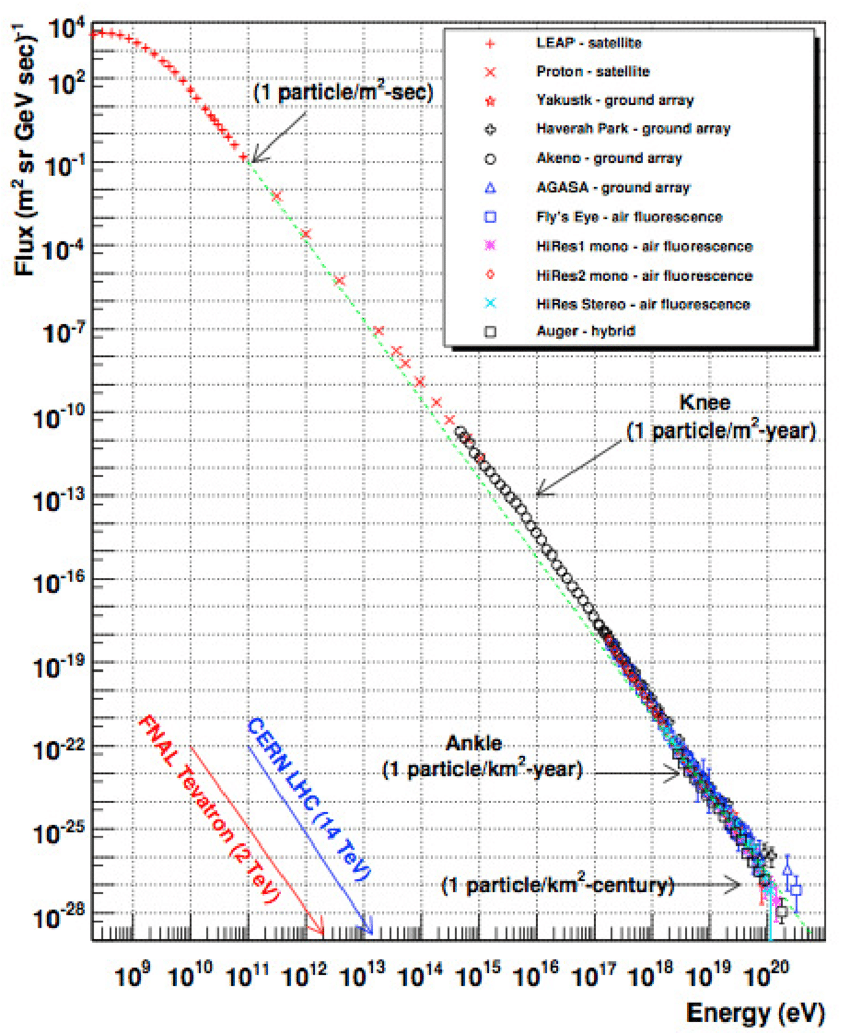
\includegraphics[width=0.45\columnwidth, height=0.4\textheight]{Figures/chapter2/Cosmicrays/CosmicRayFluxVersusParticleEnergy.png} 
}    
\subfigure[] { \label{CosmicRaysComponentsFlux}    
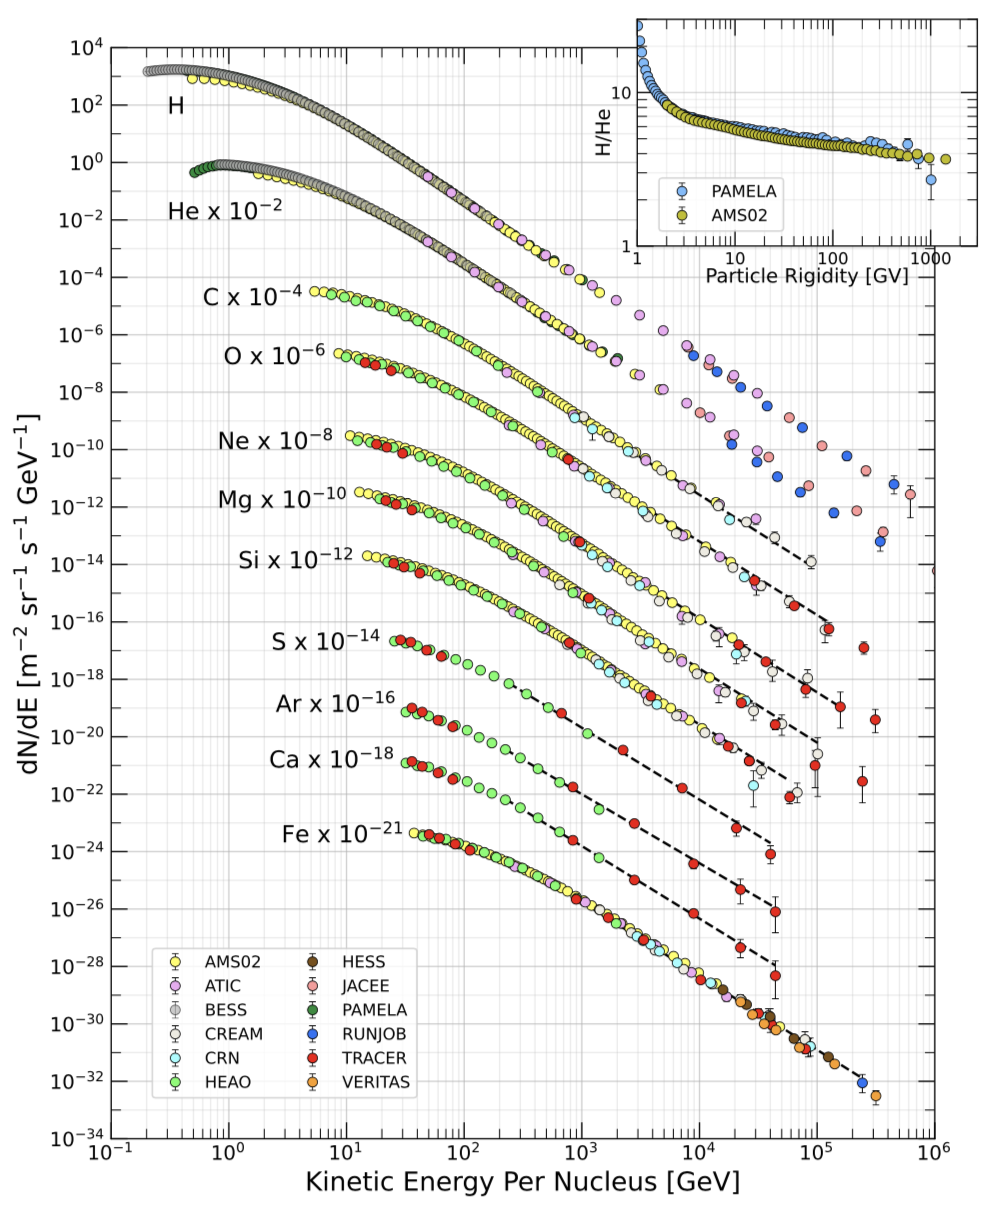
\includegraphics[width=0.45\columnwidth, height=0.4\textheight]{Figures/chapter2/Cosmicrays/CosmicRaysComponentsFlux.png}    
}    
\caption[Cosmic ray spectrum and components]{a) Cosmic ray spectrum has a wide range in flux and energy \cite{CosmicRaysKneeAndAnkle}, the knee is at around 1 PeV and the ankle is at 4 EeV. b) The fluxes of different components of cosmic rays follow a universal power law trend \cite{PDG2020}. }
\end{figure}

% Primary and secondary cosmic rays
There are two kinds of cosmic rays: primary and secondary. Primary cosmic rays are produced in astrophysical sources, while secondary cosmic rays are produced from the interactions between the primary cosmic rays and the interstellar medium. Primary cosmic rays mainly comprise protons, electrons, He, C, O, Ne, Mg, Si, Fe and others. Secondary cosmic rays consist of mainly positrons, antiprotons, Li, Be, B, F, and others. The precise measurement of cosmic rays can provide information about the astrophysical sources and also the propagation processes as well. \par

%都有:N, Na, Al,
\begin{comment}  %% AMS publication 
Primary iron cosmic rays are the most abundant heavy nuclei beyond silicon. They are thought to be mostly produced and accelerated in astrophysical sources. Iron interaction cross sections with the interstellar medium (p, He) are significantly larger than those of lighter nuclei (He, C, O, Ne, Mg, and Si). Therefore, iron nuclei interact much more with the interstellar medium during propagation. Precise knowledge of the iron spectrum in the GV–TV rigidity region provides important information on the origin, acceleration, and propagation processes of cosmic rays in the Galaxy [1]. Previously, the precision measurements of the primary cosmic ray He, C, and O fluxes and Ne, Mg, and Si fluxes with the Alpha Magnetic Spectrometer experiment (AMS) have been reported [2,3]. These measurements revealed an identical rigidity dependence of the He, C, and O fluxes above 60 GV and their deviation from a single power law (hardening) above ∼200 GV. The AMS results also revealed unexpected differences in the rigidity dependence of the Ne, Mg, and Si fluxes compared to the He, C, and O fluxes. To date, iron nuclei (Z 1⁄4 26) are the highest charge cosmic rays measured by AMS. The rigidity dependence of the iron flux compared with that of lower-charge primary cosmic rays provides new insights into the origin and propagation of cosmic rays [4,5].

Carbon nuclei in cosmic rays are thought to be mainly produced and accelerated in astrophysical sources, while boron nuclei are entirely produced by the collision of heavier nuclei, such as carbon and oxygen, with nuclei of the interstellar matter. Therefore, the boron to carbon flux ratio (B=C) directly measures the average amount of interstellar material traversed by cosmic rays.
\end{comment}


% all the components follow a power law
Cosmic rays consist of many components. For primary cosmic rays, ~89\% are protons, 10\% are helium nuclei and around 1\% are heavy elements. In figure \ref{CosmicRaysComponentsFlux} the fluxes of different cosmic ray components are shown. A universal power law spectrum is observed in all kinds of cosmic rays, which supports the assumption of a general electro-magnetic acceleration mechanism, though small differences still need to be investigated. With the efforts of different measurements, the fluxes of cosmic ray components have been measured for a large energy range.     \par

\begin{figure}[h] 
\centering
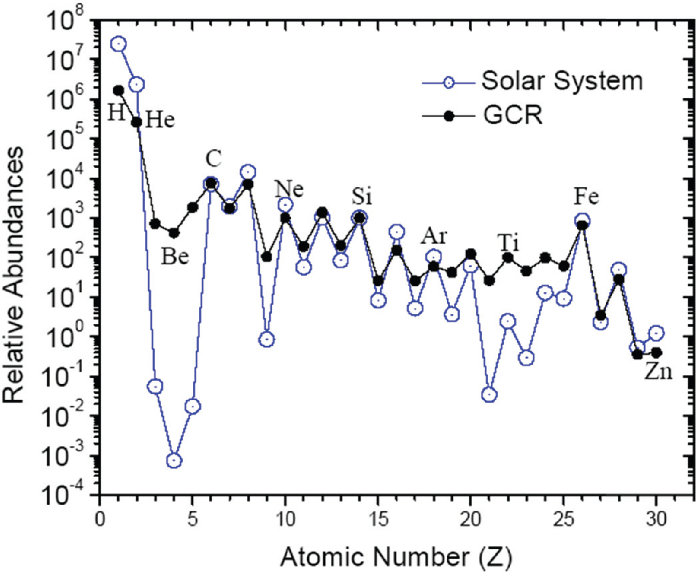
\includegraphics[width=0.9\textwidth, height=0.45\textheight ]{Figures/chapter2/Cosmicrays/Galactic-cosmic-ray-relative-abundances-compared-with-the-Solar-System-ones-The-curves.png}
\caption[Element abundances between the GCR and the solar system]{A good agreement of element abundances between the GCR and the solar system is shown \cite{ElementAbundanceOfCosmicRays_OriginalACE}, except some differences like over-abundance of H and He in solar system, excess of Li, Be, B in GCR and others.}
\label{ElementAbundanceOfCosmicRays}
\end{figure}

% 
In figure \ref{ElementAbundanceOfCosmicRays}, the abundances of the galactic cosmic rays (GCR) arriving near Earth compared to the ones of the solar system are shown. In general, there is good agreement between these two kinds of abundances, the differences illustrate the part of secondary production of cosmic rays. The reduced abundance of the galactic cosmic hydrogen and helium is due to the effects of the solar magnetic field. Due to the spallation and interactions of the cosmic rays, the C, N and O nuclei would break into elements of lower mass, namely Li, Be, and B. This fact explains the higher abundances of Li, Be and B in the GCR.  

%% ground and space measurement(待定)







\section{Sources of cosmic rays}
% Source of cosmic rays (explain why SNR can produce (see Fabian), and why it's power law) (Mertsch PPT)

%% Introduction
Traditionally, the supernova remnants (SNRs) are considered to be the main source of cosmic rays. This idea was firstly suggested by Baade and Zwicky in 1934 \cite{CosmicRaysFromSuperNova}. Apart from SNR, some other sources can also contribute to cosmic rays production, like pulsars can produce electron and positron pairs then accelerate them in the pulsar wind nebula (PWN), or dark matter can produce additional positrons and antiprotons from annihilation. Therefore, a high precision measurement of the cosmic ray flux is certainly a probe to understand the sources of cosmic rays. \par

%% supernova and supernova remnant 
A supernova is a stellar explosion event that can expel several solar masses of material with very high speed. There are mainly two mechanisms of supernova creation \cite{SupernovaClassification}: a) a white dwarf accretes matter from a companion star until it reaches the Chandrasekhar mass limit and then a nuclear fusion is triggered, and b) a massive star undergoes gravitational core collapse. During a supernova explosion, matter is ejected and accelerated at velocities of a few percent of the speed of light. As the ejected material travels faster than the speed of sound in the Interstellar Medium (ISM), it creates an expanding shock wave that sweeps up the interstellar material of gas and dust creating a "supernova remnant" \cite{SupernovaRemnants}. \par

%% Cosmic rays accelerated from the supernova remnant 
Charged particles can be absorbed into the supernova remnant and be confined in it. They gain energy and are accelerated while trapped in the supernova remnant until their energy is large enough to escape from it. The acceleration mechanisms are called "First Order Fermi Mechanism" and "Second Order Fermi Mechanism". The first one describes the particles crossing the shock front repeatedly gaining energy \cite{FirstFermiAcceleration}. The second one describes the acceleration from the particle collisions with magnetic clouds in the interstellar medium \cite{SecondFermiAcceleration}. These acceleration processes in the supernova remnant eventually lead to a power law energy spectrum.  \par

%% Pulsars generate supernova remnant  
Apart from the SNRs, pulsars can also produce high energy cosmic rays. Pulsars are rapidly rotating neutron stars with a strong magnetic field. A PWN is usually formed around a pulsar within the shell of a supernova remnant, where electrons and positrons can be produced by pair production \cite{PulsarGenerateCosmicRays, PulsarGenerateCosmicRays2}. The shock of the PWN with the surrounding matter can accelerate these charged particles to very high energies \cite{PulsarPWN, PulsarAccelerateCosmicRays}. This effect results in an important contribution to the cosmic electron and positron spectra in the high energy range. \par

%% Source of antiproton (Interactions and Dark Matter)
Since particles are produced via pair production and proton (antiproton) is much heavier than electron (positron), pulsars can produce positrons while antiprotons can not be produced by pulsars \cite{PulsarProducePositronOnly, PulsarProducePositronOnly2}. Therefore, the contribution of cosmic antiprotons to the cosmic ray spectrum, can only result from the interactions between the primary cosmic rays and the ISM. Based on this, some models give the predictions of the antiproton flux or antiproton to proton flux ratio purely from secondary production \cite{TimeAveragedPbarRatioPaperSecondaryProduction1, TimeAveragedPbarRatioPaperSecondaryProduction2}. By comparing the measurement of the cosmic antiproton, if an excess in the cosmic antiproton is observed, different sources of antiproton production, like dark matter should be investigated \cite{CosmicAntiprotons, CosmicAntiprotons2,CosmicAntiprotons3}. For example, dark matter can produce additional positrons and antiprotons via annihilation besides secondary production, the additional components from dark matter plus the secondary production could be used to fit the measured cosmic antiproton spectrum \cite{AntiprotonFromSecondaryAndDarkMatterModel}. In summary, by measuring the antiproton spectrum precisely, the sources of cosmic antiprotons can be studied.  
     
     
     
     
     
     


\section{Propagation}

% Cosmic ray propagating in the galaxy
\subsection{Cosmic rays propagating in the galaxy}
When the accelerated cosmic rays leave the SNRs, they travel through the Galaxy and then interact with the ISM producing secondary cosmic rays. By hadronic production, antiprotons can be generated. Positrons and electrons lose their energy by bremsstrahlung and synchrotron radiation in the interaction collisions. Due to their charge, cosmic rays are scattered on the magneto-hydrodynamic (MHD) waves, so their trajectory is deflected from a straight line. The path of cosmic rays can be described by a diffusion process. The effects of this diffusion, as well as other physical effects, can be quantitatively described by the transport equation \cite{CosmicRayPropagationEquation}:     

\begin{equation}  
\frac{ \partial \psi(\vec{r},p,t)}{\partial t} = q(\vec{r},p,t)  + \vec{\nabla} \cdot  (D_{xx} \vec{\nabla} \psi - \vec{V}\psi) + \frac{\partial}{\partial p}p^2 D_{pp} \frac{\partial}{\partial p} \frac{1}{p^2}\psi - \frac{\partial}{\partial p } \left [ \dot p \psi - \frac{p}{3}(\vec{\nabla} \cdot \vec{V}) \psi \right ] - \frac{1}{\tau_{f}}\psi - \frac{1}{\tau_{r}}\psi
\label{PropagationEquation}
\end{equation}

where $\psi(\vec{r},p,t)$ is the density of cosmic rays at point $\vec{r}$ with momentum p. The terms of the equation describe different physical processes and are explained here:

\begin{itemize}
\item $q(\vec{r},p,t)$ denotes the source term, that includes the primary sources, and the contributions from spallation and decay processes.
\item $D_{xx}$ is the spatial diffusion coefficient that describes the scattering off the magneto-hydrodynamic waves.
\item $\vec{V}$ is the convection velocity. The galactic winds cause an additional convective transport.
\item $D_{pp}$ is the momentum diffusion coefficient. Apart from the spatial diffusion process, charged particles traveling in MHD waves undergo stochastic re-acceleration that can be described by the momentum diffusion coefficient.
%\item $\vec{\nabla} \cdot \vec{V}$ denotes the adiabatic momentum change, this term is caused by scattering off inhomogeneities of the magnetic field. 
\item $\vec{\nabla} \cdot \vec{V}$ denotes the adiabatic momentum change, this term is the work against the pressure of the interstellar gas.
\item $\tau_{f}$ and $\tau_{r}$ are the time scales of fragmentation and radioactive decay respectively.
\end{itemize}

For each particle type a propagation equation is used, leading to a very complex system of differential equations. To solve these equations analytically is impossible, therefore numerical calculations are more practical, like Monte-Carlo based approaches. Software numerical tools that are widely used to obtain the solution of the transport equation are the following: GALPROP \cite{GALPROP}, USINE \cite{USINE}, and DRAGON \cite{DRAGON}.  \par

Alternatively, it is possible to solve simplified approximations of Eq. \ref{PropagationEquation}. The basic assumption is that the galaxy is a box where particles can freely propagate while undergoing only elastic scattering. In this case, the density of cosmic rays does not depend on the location within the box. At the edge of the box, the particles are reflected with a probability $1-P_\mathrm{esc}$, and the $P_\mathrm{esc}$ is the probability of escaping to the outside of the box. As a consequence, the diffusion term can be replaced by escape time $\tau_\mathrm{esc}$. With this assumption, the transport equation can be simplified as:

\begin{equation}  
\frac{ \partial \psi(\vec{r},p,t)}{\partial t} = \psi_{0}(p) \cdot \delta(t) - \frac{\psi(p,t)}{\tau_\mathrm{esc}}
\end{equation}

where $\tau_{esc}$ is escape time which represents the constant escape probability, $\psi_{0}(p)$ is the injection homogenous source of particles at the time t=0. This simplified approximation is called the Leaky-Box model \cite{LeakyBoxModel} and its solution is:

\begin{equation}  
\psi(p,t) = \psi_{0}(p)\rm{exp}(-\frac{t}{\tau_\mathrm{esc}}) 
\end{equation}


% Cosmic ray propagating in the heliosphere
\subsection{Cosmic ray propagating in the heliosphere}
%% Heliosphere: sun --> solar wind --> HMF and HCS --> termination shock
The Sun is continuously ejecting from its upper atmosphere a stream of charged particles when the energy of those particles surpasses the escape limit, this form the solar wind \cite{SolarWind1, SolarWind2}. The solar wind plasma drags outwards the solar magnetic field forming the HMF \cite{HeliosphericMagneticField}. Because of the rotation of the Sun, the HMF has a spiral shape which is called Parker spiral, and the shape of the HMF is changing with the Sun's activity. The opposite polarity of HMF is separated by the heliospheric current sheet (HCS). The charged particles of the solar wind reach speeds of around 400 km/s, meaning they are faster than the speed of the magnetosonic wave, therefore they are supersonic. After traveling for some distance and encountering the interstellar medium, the speed of the solar wind abruptly decelerates and becomes subsonic at the termination shock \cite{HeliospherePaper}. Figure \ref{Heliosphere} shows a diagram of the heliosphere. The Voyager 1 probe became the first spacecraft to cross the termination shock in 2004 and later in 2012 to encounter the heliopause \cite{Voyager1Paper}. As shown in Figure \ref{Voyager1}, the solar wind particle rate dramatically decreases after reaching the outer border of the heliosphere.

\begin{figure} \centering   
\subfigure[] { \label{Heliosphere}    
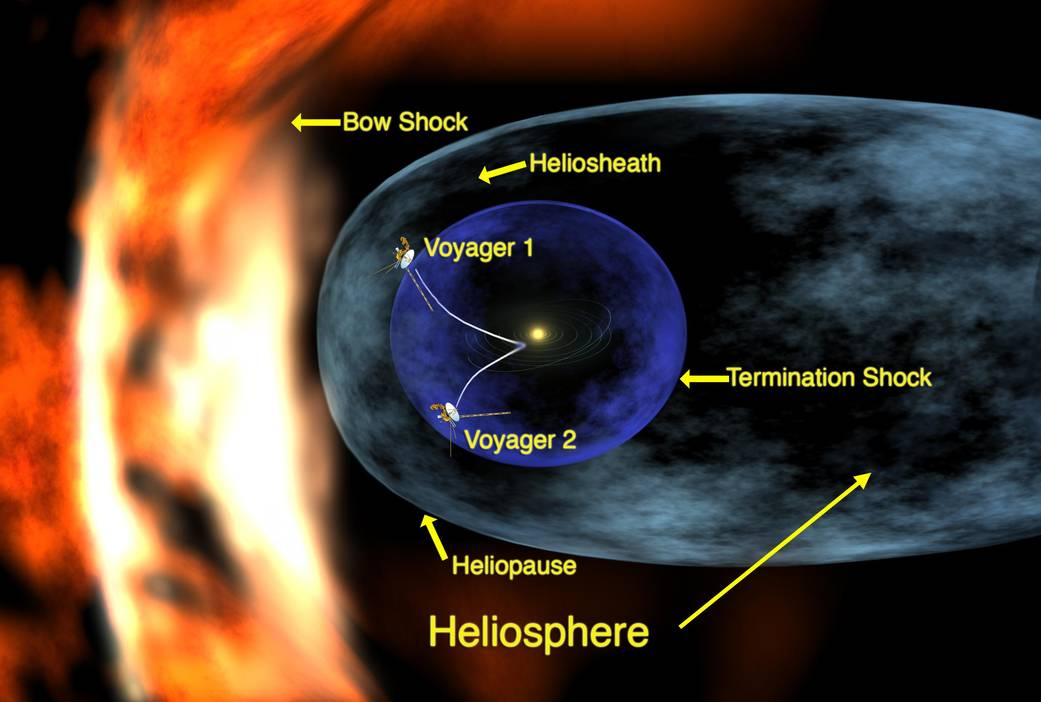
\includegraphics[width=0.47\columnwidth, height=0.26\textheight]{Figures/chapter2/Propagations/Heliosphere.jpg} 
}    
\subfigure[] { \label{Voyager1}    
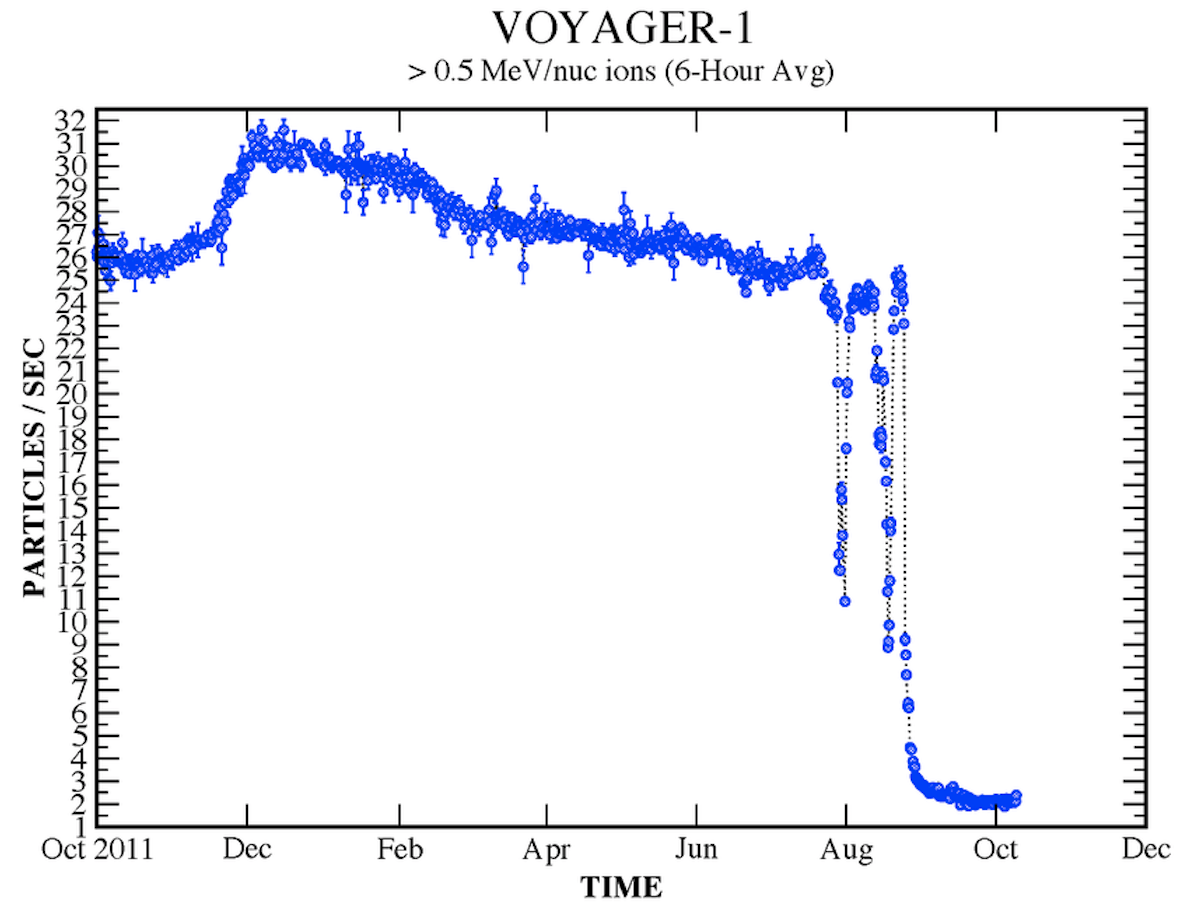
\includegraphics[width=0.47\columnwidth, height=0.26\textheight]{Figures/chapter2/Propagations/Voyager1.png}    
}    
\caption[Heliosphere and Particle rate detected by Voyager 1.]{a) Diagram of the heliosphere. Credit: NASA/Walt Feimer; b) Particle rate detected by Voyager 1 (from October 2011 through October 2012) \cite{WikiVoyager1ReachHeliosphere}.}     
\end{figure}

% sunspot difination -> sun rotation --> polartiy reverse 11 years (22 years cycle) --> the HMF shape change with sun activity
Sunspot is a spot that looks darker than the surrounding areas on the Sun's photosphere, which represents solar activity. During the solar maximum, the number of sunspots reaches the maximum and the polarity of the HMF reverses. The sunspot number changes in a cycle of 11 years. Considering the polarity, a full cycle of the Sun's activity is 22 years \cite{SolarCycle}. The solar cycles have been counted since 1755 and now we are in solar cycle 25 \cite{SolarCycleFirstObservation1, SolarCycleFirstObservation2}. \par


% propagation in the heliosphere 
When galactic cosmic rays enter the solar system, they travel through the heliosphere first before reaching the Earth. The propagation process is similar to the propagation in the galaxy but the diffusion coefficient is orders of magnitude smaller. Since the full transportation equation can not be solved analytically, a simplified model proposed in \cite{ForceFieldApproximationPaper} is usually used and it describes the process as the diffusion through the HMF. In this model, under the force-field approximation, an analytical solution of the one-dimensional steady-state equation is derived, which relates the GCR spectrum measured at Earth $J$ and in the local interstellar space  $J_\mathrm{LIS}$:  

\begin{equation}
J(T_{\rm{E}}) = \frac{T_{\rm{E}}(T_{\rm{E}}+2M)}{T_{\rm{HP}}(T_{\rm{HP}}+2M)} J_\mathrm{LIS}(T_{\rm{HP}})
\end{equation}

where the $M$ is the particle mass, $T_{\rm{E}}$ and $T_{\rm{HP}}$ are the kinetic energies of the particle at Earth and at the heliopause. $T_{\rm{HP}}=T_{\rm{E}} + Z \phi$, and $\phi$ is called modulation potential, which depends on the solar wind speed and the diffusion coefficient. Since the solar activity and the physical status of the heliopause vary following the 22-year cycle, the measured GCR spectrum at Earth also shows a variation of the 22-year cycle. This is called solar modulation. 

%   sunspot vs CRs: anti-correlated
\begin{figure}[t]
\centering
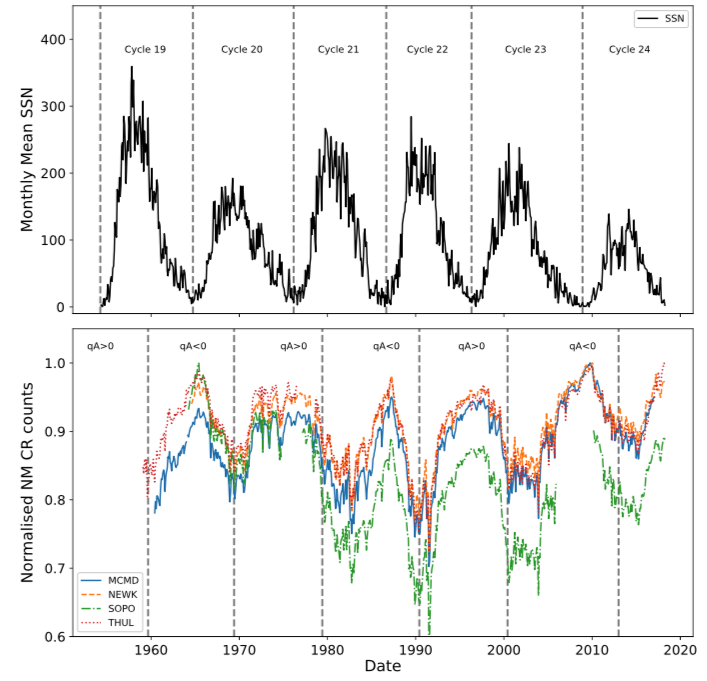
\includegraphics[width=0.80\textwidth, height=0.5\textheight]{Figures/chapter2/Propagations/NeutronMonitor.png}
\caption[Cosmic rays intensity and Monthly mean sunspot numbers.]{Bottom figure: The cosmic rays (CR) intensity recorded by neutron monitor (NM) counts from four different stations (MCMD = McMurdo, NEWK = Newark, SOPO = South Pole, THUL = Thule). The vertical lines show the approximations of epochs of solar magnetic-field polarity reversals and qA is the solar polarity. Top figure: Monthly mean sunspot numbers (SSN) over the latest six solar cycles. The vertical lines show the beginning of each solar cycle. The figure is taken from \cite{NeutronMonitor}. }
\label{NeutronMonitor}
\end{figure}

In the figure \ref{NeutronMonitor}, the different ground-based cosmic neutron measurements and the monthly mean sunspot numbers are shown. The cosmic neutron counts show the intensity of hadronic cosmic rays, which indicate the measured cosmic rays at Earth. The sunspot numbers are correlated to solar activity. When the GCRs enter the solar system, they interact with the solar wind and magnetic fields. A large solar activity reduces the cosmic rays and vice versa. Therefore, the sunspot numbers and the cosmic neutron counts are anti-correlated. By measuring the cosmic ray flux over a long period of time, the impact of solar activity can be studied. Until recently, the only continuous cosmic ray flux measurements over a long period of time have been performed only for the dominant components of the cosmic spectrum like protons, helium, electron or neutrons produced in cascades in the Earth’s atmosphere. There is no continuous measurement of rare cosmic ray components like antiproton. Since the AMS-02 experiment has been collecting cosmic data for 10 years, the first time-dependent antiproton measurement can be achieved.  \par 

% Drift--->Particle Sign Different
Due to the sign of charged particles, they drift differently in different polarities. For example, in positive polarity, the positively charged particles drift toward the Sun from the heliospheric poles and outwards to Earth. While the negatively charged particles drift arriving at Earth inwards along the HCS. This leads to different diffusion processes in the heliosphere. This charge-dependent modulation results in a different behavior between antiprotons and protons, furthermore, the antiproton to proton flux ratio behaves differently in opposite polarity periods. Similarly, positron and electron also behave differently due to opposite charge signs. In the time-dependent positron to electron flux ratio measurement by AMS-02 \cite{AMSElectronPositronPaper}, this can be observed. Also, the reversal of polarity is not easy to be determined clearly. The measurement of the positron to electron flux ratio can provide information about the reversal period.


% 太阳的结构,可以形象的称之为“里三层、外三层”模型。里三层,是指太阳内部的核反应区(日核)Core、辐射区Radiative zone、对流区(对流层)Convective zone;外三层,是指太阳大气的光球层Photosphere、色球层Chromosphere、日冕层Corona。
% 太阳磁场主要在太阳大气层 - 光球Photosphere、色球Chromosphere 和 日冕Corona低层中
% 太阳磁场还有周期性的磁场反转,与黑子的出现地点有所关连,黑子的出现地点会从太阳极区渐渐移往赤道地区,可以用蝴蝶图来表示,呈现约11年的周期变化,太阳磁场也是约每11年反转一次






\section{Cosmic antiprotons measurement}

%% First two antiproton experiments
Cosmic rays were discovered in 1912 \cite{NobelCosmicRay}, the antiproton was discovered in 1955 \cite{NobelAntiproton}, and the first measurements of cosmic antiproton component were performed in 1979 \cite{CosmicAntiprotonBogomolov1979, CosmicAntiprotonGolden1979}, when two pioneering balloon flight experiments published their results about cosmic antiprotons independently. The first one was carried out by Bogomolov et al. and the data taking was from 1972 to 1977 by three individual flights, the residual air was 11 g/cm$^2$ so a correction was needed. The result showed two candidates of cosmic antiprotons in the kinetic energy range of 2-5 GeV. The second one was carried out by R. L. Golden et al. in Palestine in Texas and the data taking was from June 21 to June 22 1979. The residual air in the flight altitude was 5.4 g/cm$^2$. The spectrometer had a superconducting magnet and the group reported 46 antiproton candidates from 5.6 to 12.5 GV. 

% Comment out
\begin{comment}
%In figure \ref{First2PbarExp}, the cosmic antiproton candidates in those two experiments are shown.
\begin{figure}[h] \centering   
\subfigure[] { \label{}    
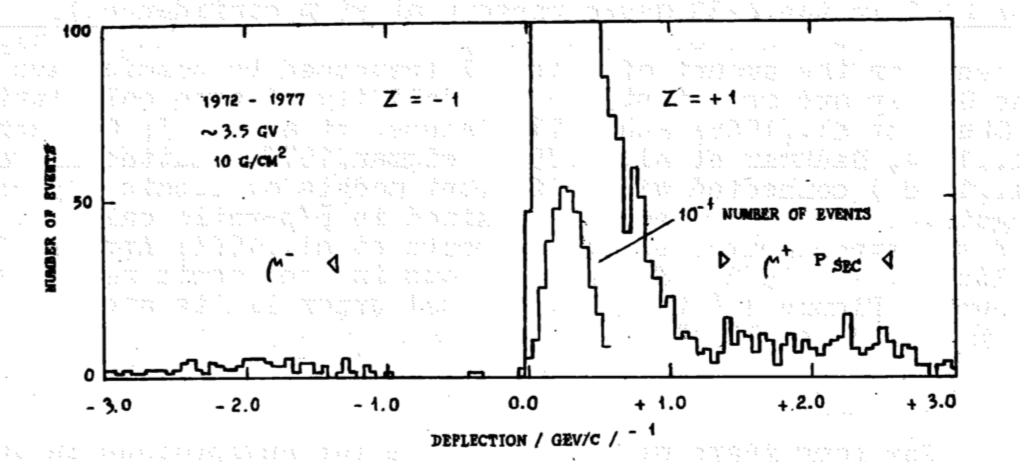
\includegraphics[width=0.45\textwidth, height=0.19\textheight]{Figures/chapter2/CosmicAntiprotonsMeasurement/Bogomolov1979.png} 
}    
\subfigure[] { \label{}    
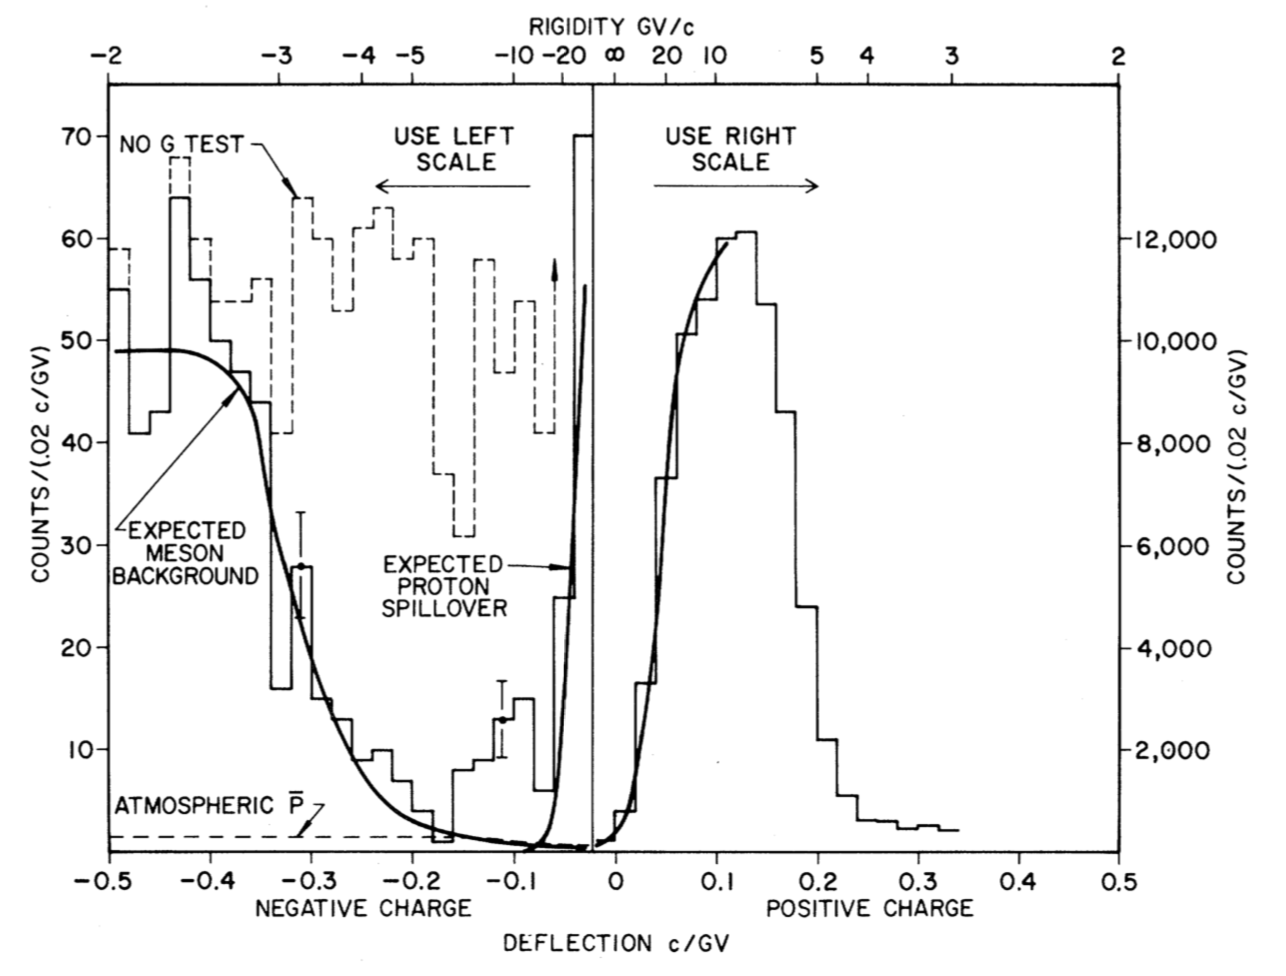
\includegraphics[width=0.45\textwidth, height=0.3\textheight]{Figures/chapter2/CosmicAntiprotonsMeasurement/Golden1979.png}    
}      
\caption{a). The antiproton signals in deflection (1/Rigidity) from the balloon flight experiment carried out by Bogomolov et al. in 1979 \cite{CosmicAntiprotonBogomolov1979}. b). The antiproton signals in deflection from the balloon flight experiment carried out by Golden et al. in 1979 \cite{CosmicAntiprotonGolden1979}}
\label{First2PbarExp}    
\end{figure}
\end{comment}

%% Bess and Pamela, AMS2016 Resul
% BESS 
After decades of effort, many cosmic ray experiments published results about cosmic antiprotons. For example, the BESS experiment, which is a balloon flight experiment \cite{BESSExperiment}, had nine successful flight campaigns since 1993. Then the apparatus was upgraded and renamed as BESS-Polar. The BESS-Polar was carried out in 2004 and 2008 respectively in the Antarctic \cite{BESSPolarExperiment1, BESSPolarExperiment2} and both flights measured the cosmic antiprotons \cite{BESSPolar1AntiprotonPaper, BESSPolar2AntiprotonPaper}. In the final result from the BESS-Polar II experiment, the group used data taken from Dec 2007 to Jan 2008 (a period corresponding to a  solar minimum) and reported the measurement of 7886 cosmic antiprotons in the kinetic energy range from 0.17 to 3.5 GeV \cite{BESSPolar2AntiprotonPaper}. 

% Comment out
\begin{comment}
Figure \ref{AntiprotoninBess2} shows the antiproton signals in $1 / \rm{\upbeta}$ versus Rigidity from BESS-Polar II.
\begin{figure}[h]
\centering
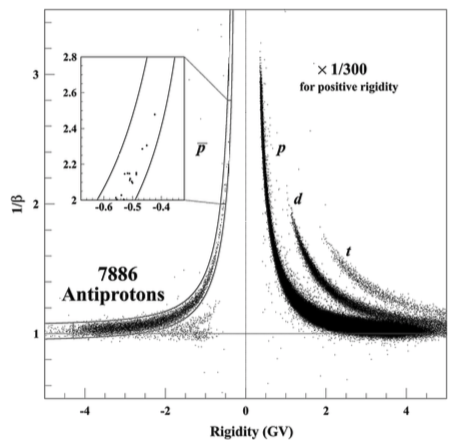
\includegraphics[width=0.5\textwidth, height=0.3\textheight]{Figures/chapter2/CosmicAntiprotonsMeasurement/AntiprotoninBess2.png}
\caption{The 7886 antiprotons signals and other components measured by BESS-Polar II in $1 / \upbeta$ versus Rigidity \cite{BESSPolar2AntiprotonPaper}.}
\label{AntiprotoninBess2}
\end{figure}
\end{comment}

%% Pamela and AMS2016
Due to the limited height of the balloon flight experiments, the correction of the residual air has to be considered to get a flux result above the atmosphere. The correction that the residual air creates can be overcome if a spectrometer is placed in space where the residual air is negligible. 

The first satellite-based cosmic antiproton measurement was performed by the PAMELA detector. PAMELA's mission lasted from June 2006 to February 2016 at a float altitude between 350 km and 610 km. The orbital period of the host satellite Resurs-DK1 was 94 min \cite{PamelaExperiment}. The PAMELA group published several antiproton results and the last one was in 2012 \cite{PamelaAntiproton100Paper, PamelaAntiproton180Paper, PamelaAntiproton350Paper} with a maximum measured energy of 350 GeV \cite{PamelaAntiproton350Paper}. This result shows a relatively flat antiproton to proton flux ratio in the high energy range, which is different from the traditional prediction of cosmic antiprotons from purely secondary production. In 2016 the AMS-02 experiment published its first result on cosmic antiprotons extending the measured rigidity range up to 450 GV using cosmic ray data collected during the first four years of its operation \cite{AMS02AntiprotonPRL2016}. The details of the AMS-02 experiment will be shown in the next chapter. \par

Apart from the experiment mentioned above, there are other balloon experiments that measured cosmic antiprotons. The antiproton flux results from these experiments are given in figure \ref{PbarFluxForDifferentExperiments}.  

\begin{figure}[h]
\centering
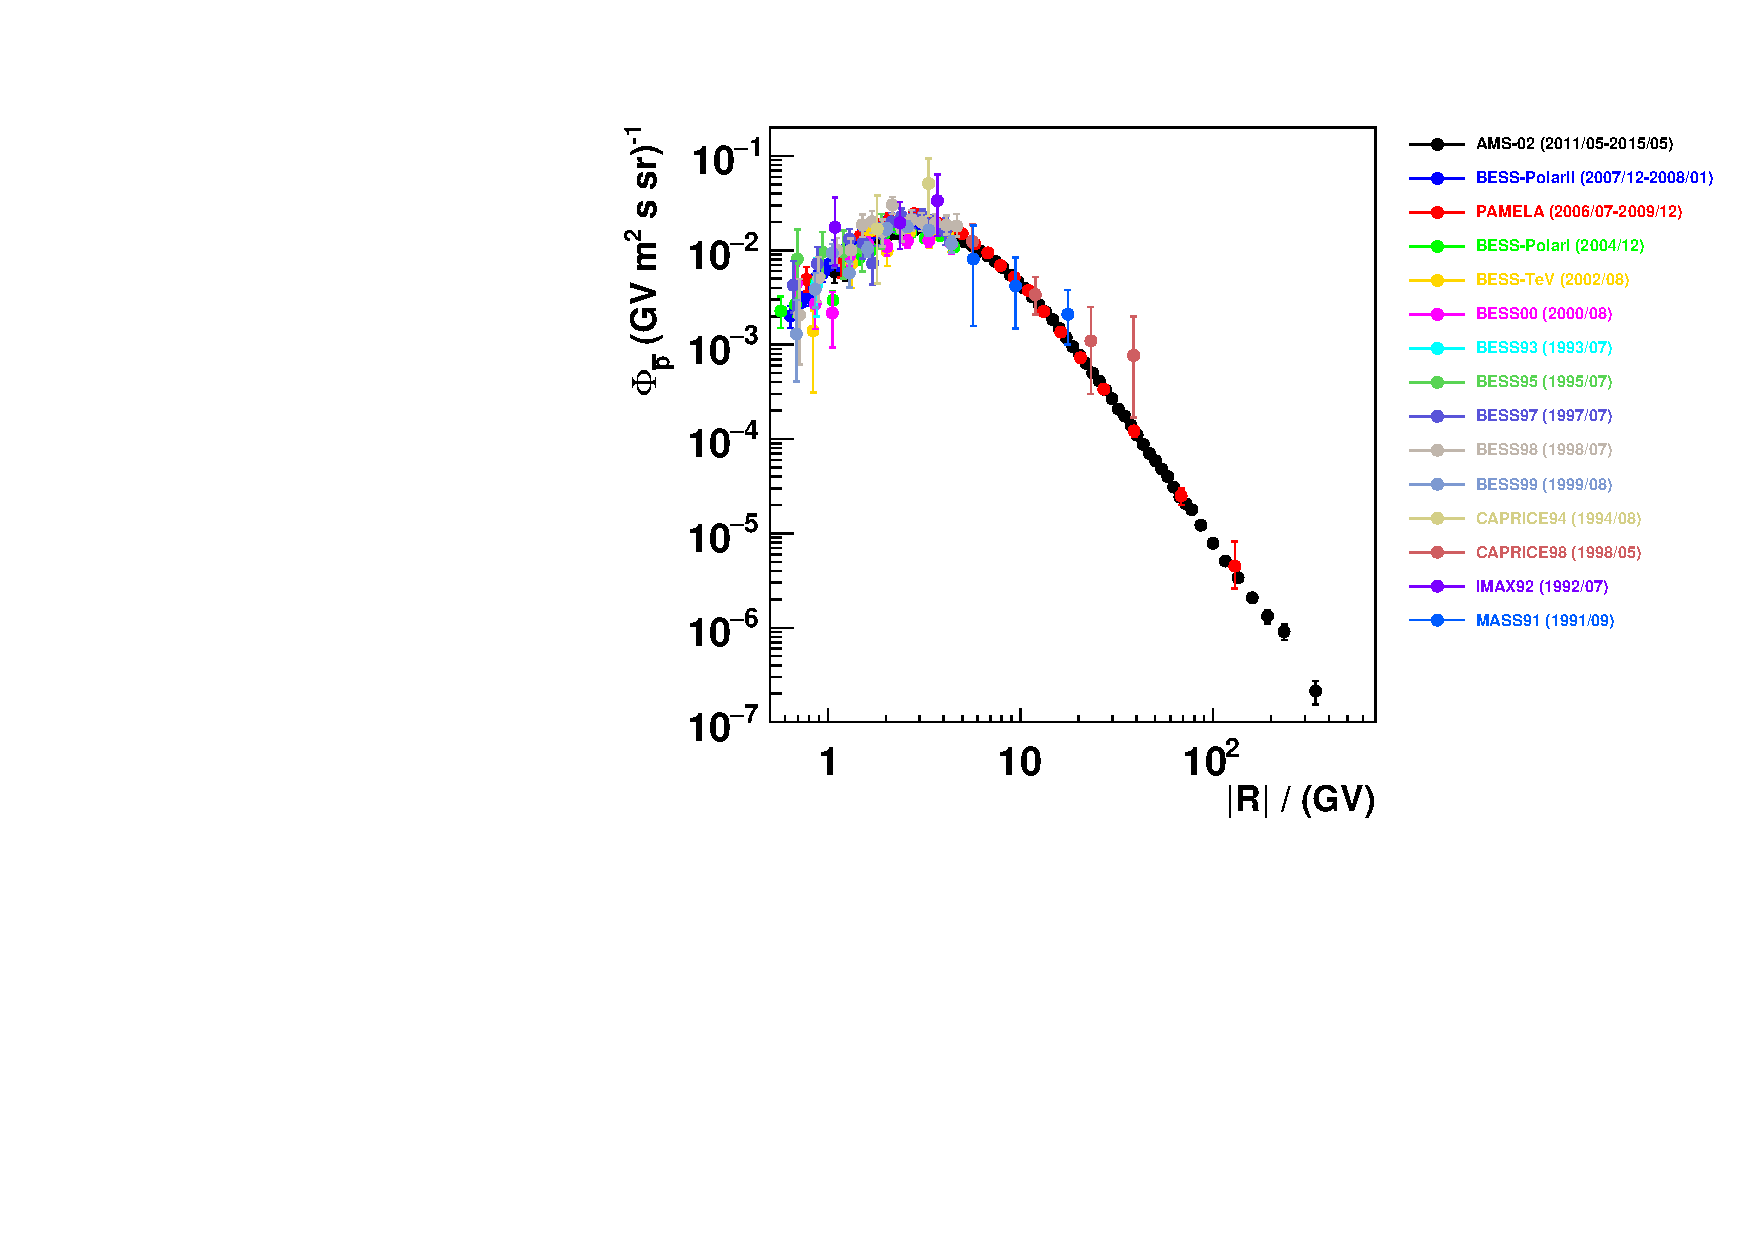
\includegraphics[width=1.0\textwidth, height=0.47\textheight]{Figures/chapter2/CosmicAntiprotonsMeasurement/PbarFluxForDifferentExperiments.pdf}
\caption[The measured antiproton flux.]{The antiproton flux measured by AMS-02 \cite{AMS02AntiprotonPRL2016}, BESS-Polar II \cite{BESSPolar2AntiprotonPaper}, PAMELA \cite{PamelaAntiproton350Paper}, Bess-Polar I \cite{BESSPolar1AntiprotonPaper}, Bess-TeV \cite{BESSTeV}, BESS00 \cite{BESS00and99}, BESS93 \cite{BESS93}, BESS95 \cite{BESS95}, BESS97 \cite{BESS97}, BESS98 \cite{BESS98}, BESS99 \cite{BESS00and99}, CAPRICE94 \cite{CAPRICE94}, CAPRICE98 \cite{CAPRICE98}, IMAX92 \cite{IMAX92}, MASS91 \cite{MASS91}. }
\label{PbarFluxForDifferentExperiments}
\end{figure}

% Pbar over P: 10^-4 so it's difficult.
Compared to antiproton measurement, the proton measurement is much easier since it is overwhelmingly dominant in cosmic rays. Many experiments have published the measurements of cosmic protons \cite{AMS02ProtonPaper, DAMPEProton2019, PAMELAProton2011, ATIC2Proton2009, CREAMIIIProton, NUCLEON-KLEMProton}. In this thesis, I will focus on the antiproton to proton flux ratio. Proton is primary cosmic ray and antiproton is believed to be secondary cosmic ray. Therefore, the antiproton to proton flux ratio is a probe to study the secondary to primary cosmic ray ratio, which can be used to investigate the source and the propagation of cosmic rays. Since the proton flux is about $10^4$ times greater than the antiproton flux, measuring the antiproton flux to 1\% accuracy requires a separation power of $\sim 10^6$. This leads to a challenge in high-energy measurement. 
   



%%%% Chapter 3 %%%%
\chpt{AMS-02 Experiment} \label{ChapterAMS02}


\section{Experiment Overview}

% AMS-01 --> AMS-02
The Alpha Magnetic Spectrometer (AMS) experiment was proposed by Nobel laureate Prof. Samuel Ting from MIT in 1994 and was soon accepted \cite{AMSProposal1994}. The goal of the experiment is to search for antimatter and dark matter in the universe
and to provide precise measurements of the fluxes for different components of the cosmic rays, which is crucial for understanding the sources of cosmic rays and their basic propagation model \cite{AMS02Goal}. \par

To test the feasibility of a particle spectrometer in space, a prototype called AMS-01 (figure \ref{AMS01Detector}) was designed, which was a simplified version of the final detector. The test flight was conducted in 1998 during the space shuttle mission STS-91 \cite{AMS01Result}, see figure \ref{AMS01TestFlight}. By collecting cosmic ray data for ten days, the test flight proved that placing and operating a spectrometer in space is possible.   \par
    
\begin{figure}[] 
\centering   
\subfigure[] { \label{AMS01Detector}    
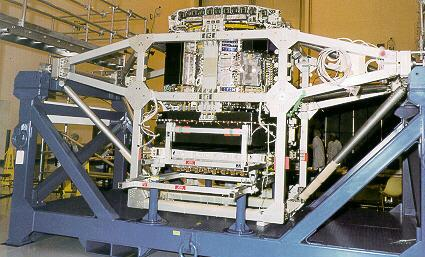
\includegraphics[width=0.5\textwidth, height=0.3\textheight]{Figures/chapter3/Overview/AMS01Detector.jpg}    
}    
\subfigure[] { \label{AMS01TestFlight}    
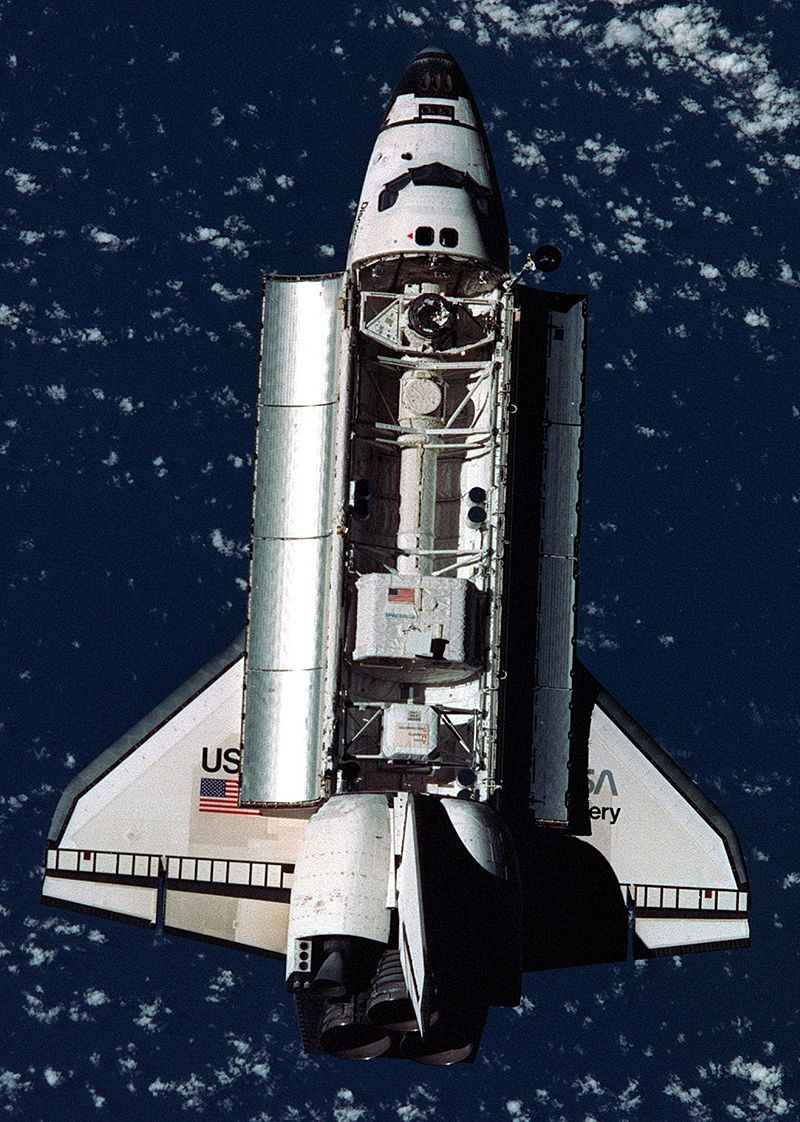
\includegraphics[width=0.4\textwidth, height=0.37\textheight]{Figures/chapter3/Overview/AMS-01.jpg} 
}    
\caption[The AMS-01 detector.]{a) The AMS-01 detector at the Kennedy Space Center (NASA) with its support structure \cite{AMS01Brochure}; b) The AMS-01 detector aboard the Space Shuttle Discovery during the STS-91 mission in June 1998 \cite{WikiAMS01Flight}.}   
    
\label{AMS01}    
\end{figure}

After several years of construction and testing, the AMS-02 detector was launched aboard the space shuttle Endeavour during mission STS 134 from Kennedy Space Center on 16 May 2011. Three days later, the detector was installed on the ISS's S3 Upper Inboard Payload Attach Site and began collecting data. Figure \ref{AMS02OnISS} shows the location of AMS-02 on the ISS. \par

\begin{figure}[]
\centering
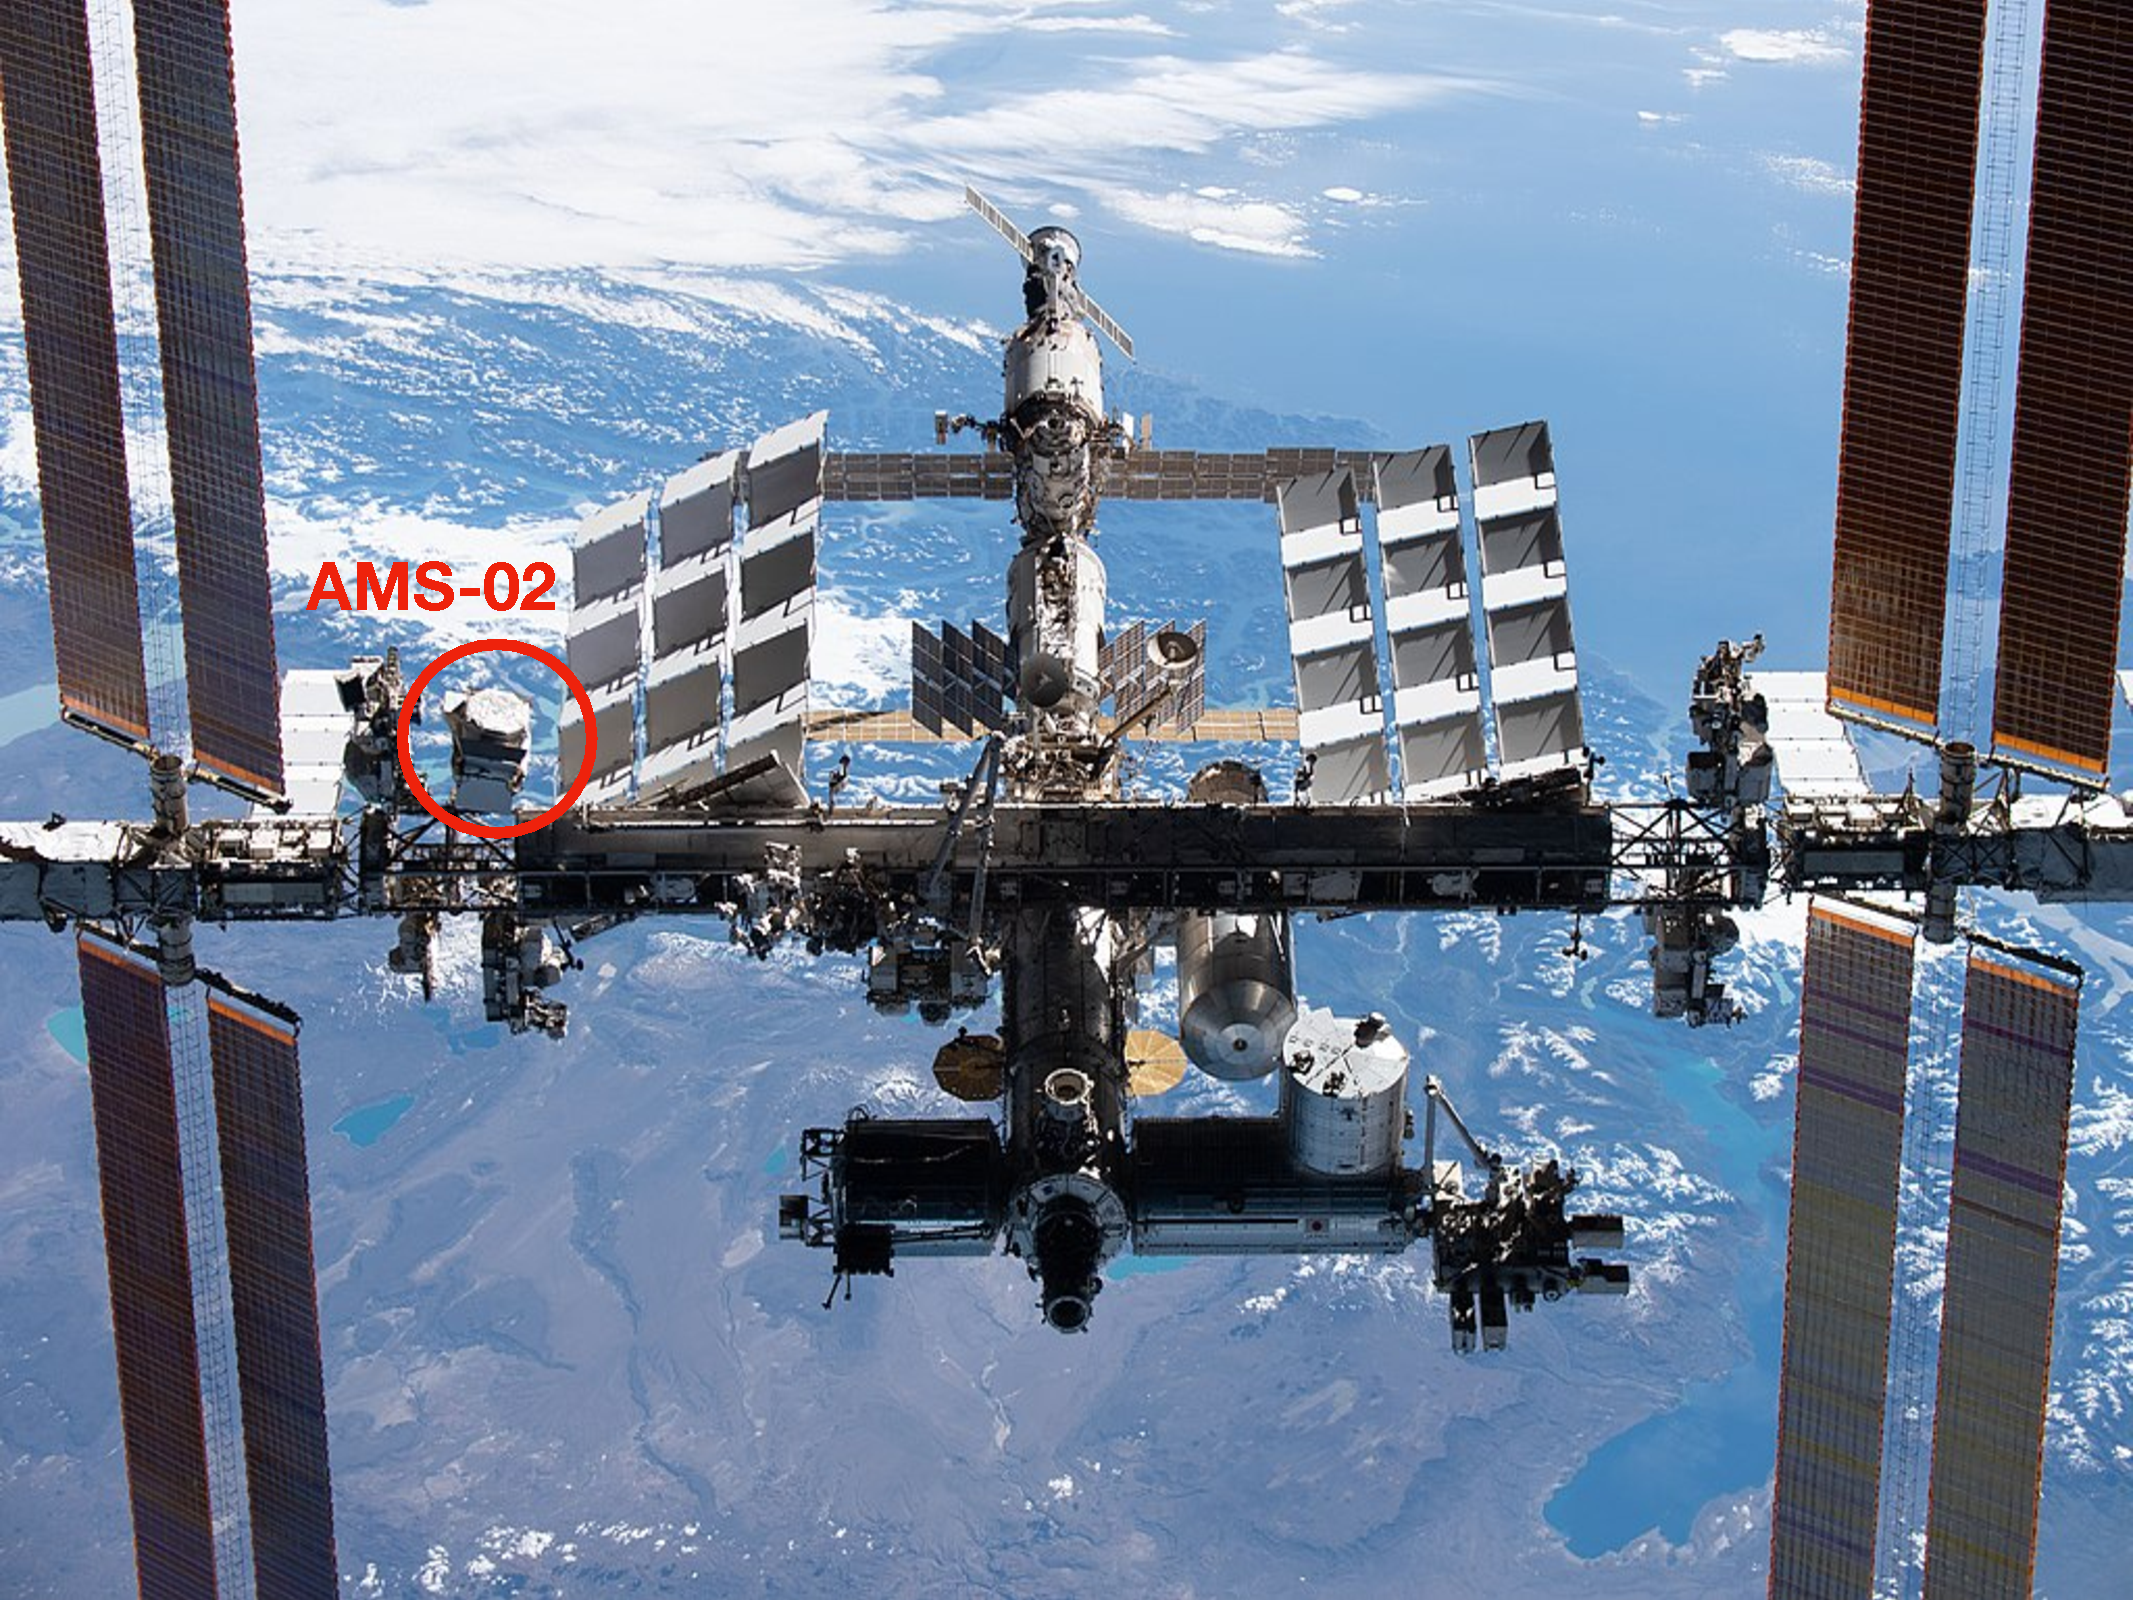
\includegraphics[width=0.8\textwidth, height=0.39\textheight ]{Figures/chapter3/Overview/AMS02OnISS.pdf}
\caption[The AMS-02 detector on the ISS.]{The AMS-02 detector mounted on the ISS S3 Upper Inboard Payload Attach Site (Image modified from \cite{wikiISS}). }
\label{AMS02OnISS}
\end{figure}

% Sub-detectors
The AMS-02 detector has a size of 5 m $\times$ 4 m $\times$ 3 m and weighs 7.5 t \cite{PhysicsReport2}. It has a permanent magnet that provides a magnetic field of 0.14 T and in combination with nine silicon tracker layers the rigidity of the cosmic particles can be measured. Within the magnet, the Anti-Coincidence Counters (ACC) are used as a veto system to reject particles entering the detector sideways. At the top of the experiment, there is a Transition Radiation Detector (TRD), which can distinguish light and heavy particles. Above and below the magnet there are two Time-Of-Flight (TOF) systems which provide the trigger and the measurements of the velocity and the charge of the particles. Below the lower part of the TOF, a Ring-Imaging Cherenkov (RICH) detector is located so the particle's velocity can be measured. At the bottom of the detector, there is an Electromagnetic Calorimeter (ECAL) which measures the energy of the particles. The geometry of all the sub-detectors is illustrated in figure \ref{AMS02Geometry}. 

\begin{figure}[]
\centering
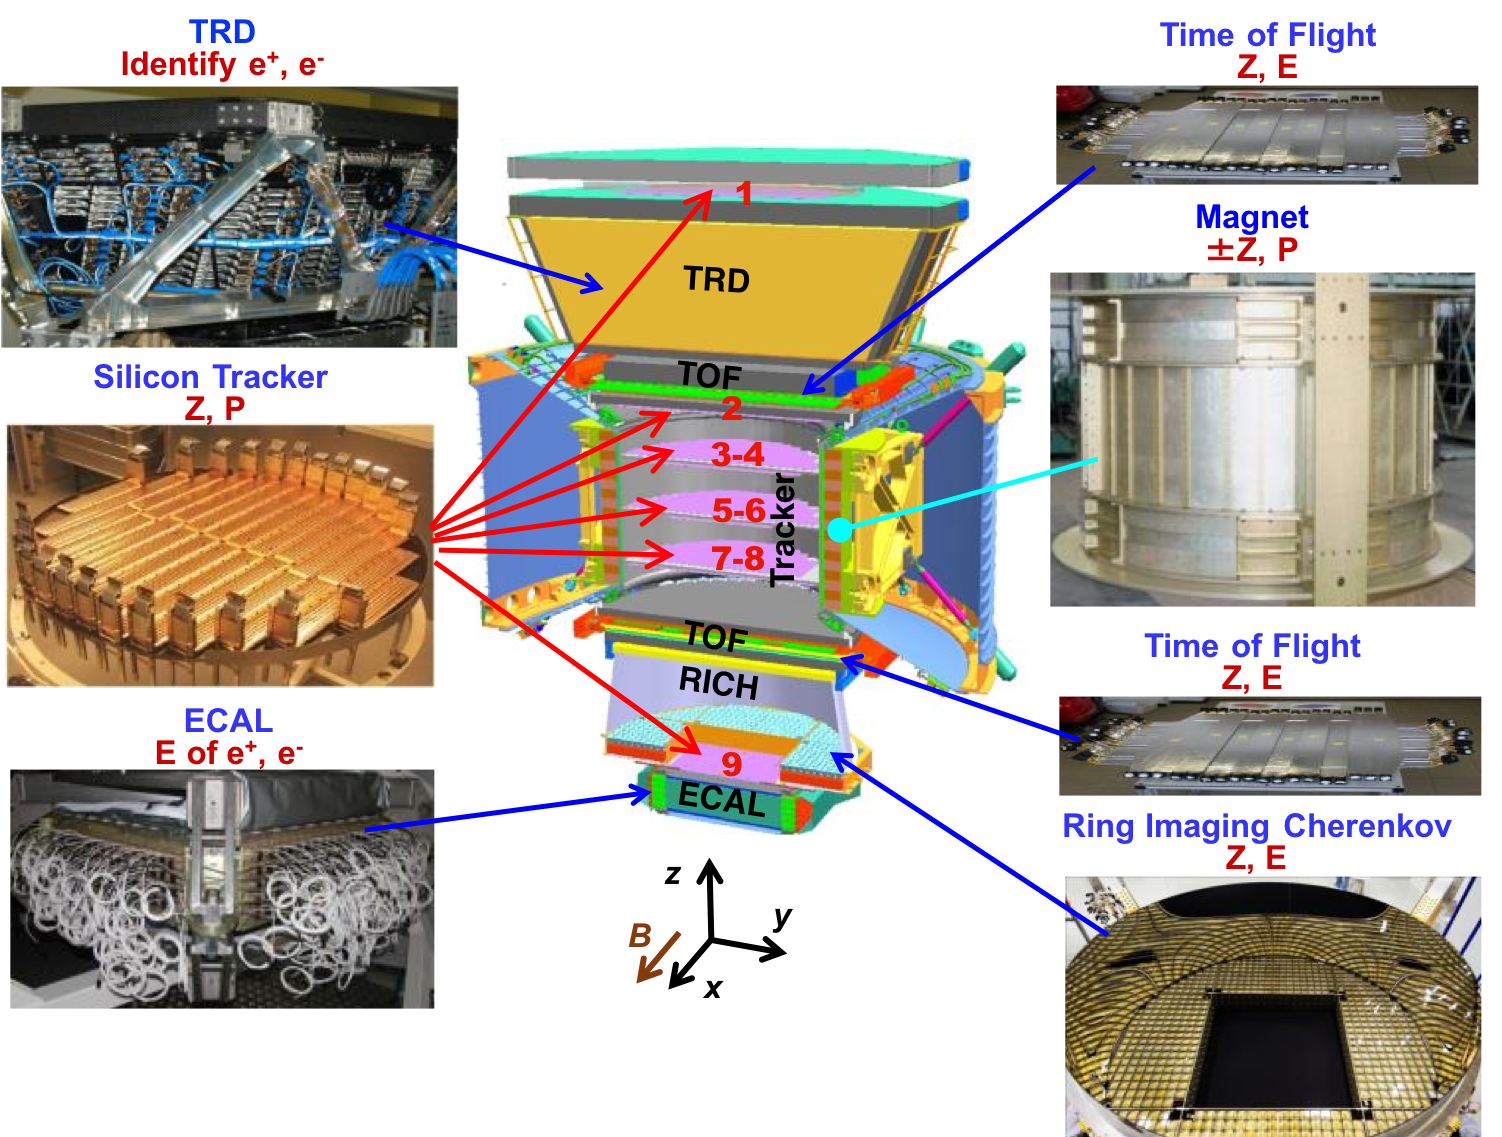
\includegraphics[width=0.8\textwidth, height=0.4\textheight ]{Figures/chapter3/Overview/AMS02Geometry.png}
\caption[Schematic view of the AMS-02 experiment.]{Schematic view of the AMS-02 experiment and all its sub-detectors \cite{AMSWebside}. }
\label{AMS02Geometry}
\end{figure}

% operations 
Detector operations have been conducted since the launch to make the experiment run smoothly. These operations can be distinguished in flight and ground operations. As part of the flight operations, the collected data is transmitted from the ISS to tracking and data relay satellites (TDRS). Then through the S (low rate) and Ku (high rate) radiofrequency bands, the data is transmitted to the White Sands Ground Terminal (WSGT) in New Mexico. Over the NASA networks, the data is then directed to the Marshall Space Flight Center (MSFC) and is written on disk. At last, the data is transmitted over the Internet and copied to the Payload Operations Control Centre (POCC) at CERN.

%The collected data is transmitted from the upper left to the lower left in this figure in a clockwise sequence. The command from the ground to the space station follows the counterclockwise sequence. In figure \ref{AMS02operations} the operation process is illustrated.
%\begin{figure}[]
%\centering
%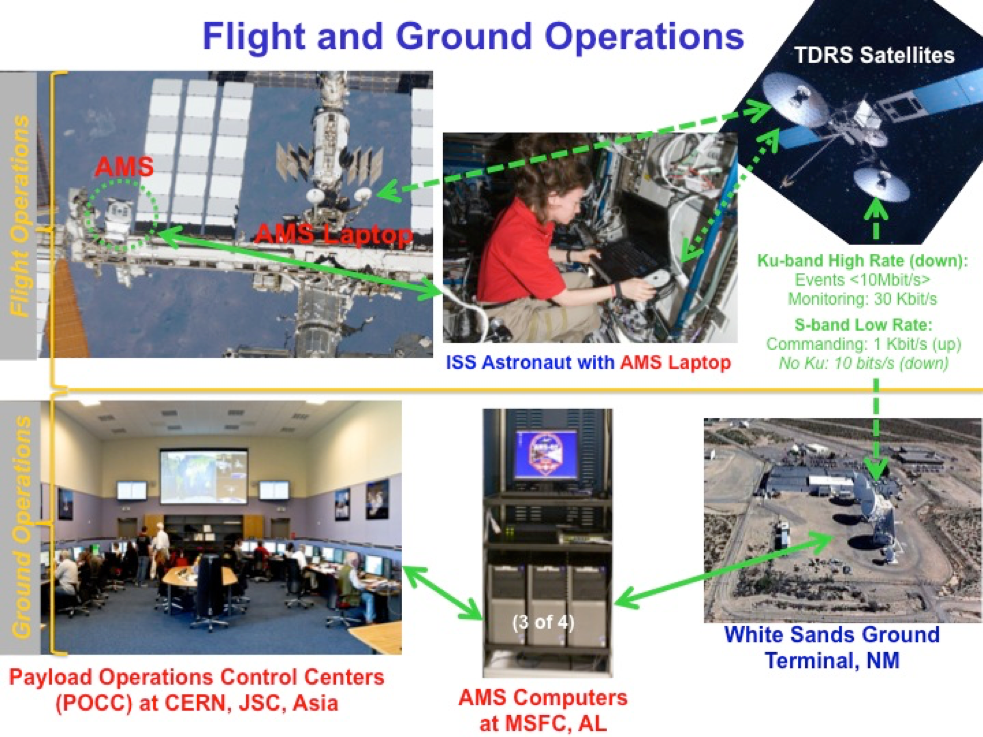
\includegraphics[width=0.8\textwidth, height=0.4\textheight ]{Figures/chapter3/Overview/Operations.png}
%\caption{A overview of AMS-02 experiment operations flow in flight and ground \cite{AMSWebside} }
%\label{AMS02operations}
%\end{figure}






  

\section{Transition Radiation Detector} \label{TRDSection}

% Definition of Transition radiation and the Characters of Transition Radiation 
The TRD can separate different particles based on the transition radiation emitted. Transition radiation is emitted when a relativistic charged particle goes through the boundary between two different mediums with different dielectric constants \cite{TransitionRadiation_Ginzburg1945}. The emitted radiation is produced due to the different solutions of Maxwell's equations of the electric and magnetic fields of the moving charged particle in these two mediums, so photons have to be emitted when the particle crosses the boundary. The intensity of the emitted photon is proportional to the Lorentz factor $\gamma$, so for a relativistic charged particle, the emitted transition radiation photons have wavelengths in the X-ray range of the electromagnetic spectrum and their direction is mostly forward. The angle between transition radiation and particle path is proportional to $1/\gamma$.    \par


% AMS TRD
The AMS-02 experiment has a transition radiation detector placed on the top of the experiment between the tracker layer one and the upper TOF layer \cite{AMS02TRDPaper1, AMS02TRDPaper2}. The TRD has 5248 proportional straw tubes; each one has a 6 mm diameter and a maximum length of 2 m. The straw tubes have double-layer kapton-aluminum foil walls of 72 $\mu$m in thickness and at their center there is a 30 $\mu$m gold-plated tungsten wire. The tubes are filled with a xenon (Xe) and carbon dioxide (CO2) gas mixture, which is supplied by two storage tanks (5 kg $\rm CO_2$ and 49 kg $\rm Xe$). When a charged particle goes through the straw tube it ionizes the $\rm{Xe}$ atoms and the produced electrons drift towards the anode wire creating an avalance of ionization proportional to the energy loss of the particle. Finally, a signal is induced on the anode wire. The $\rm CO_2$ quenches the environment and reset it to its initial state. So far, no detectable large leak in the AMS-02 TRD gas system has been observed. Due to gas diffusion across the tube walls, the loss of $\rm CO_2$ is around 0.47 g/day and the loss for $\rm Xe$ is negligible. This ensures that the TRD can be stably operated until 2039.  \par

The TRD tubes are assembled in 328 modules and one module has 16 tubes. Furthermore, all these modules are mounted in 20 layers. Twelve layers are placed along the Y axis in the middle of TRD, four layers are placed along the x-axis on top, and four layers along the x-axis are on the bottom. In figure \ref{TRDConstruction}, the TRD and its support structure are shown.  \par

\begin{figure}[t]
\centering
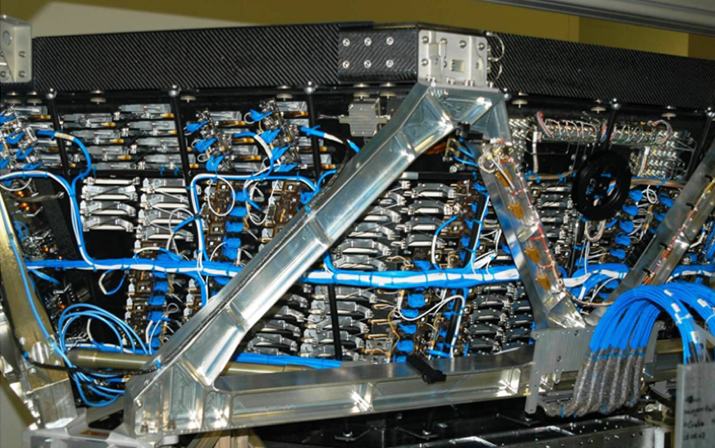
\includegraphics[width=0.8\textwidth, height=0.4\textheight ]{Figures/chapter3/TRD/TRDConstruction.png}
\caption[The TRD and its support structure during construction.]{The TRD and its support structure during construction \cite{AMSWebside}.}
\label{TRDConstruction}
\end{figure}

% TRD transition radiation 
Figure \ref{TRDdEdXPlot} shows an illustration where an electron and a proton go through one TRD layer. The upper part of the layer is a 20 mm thick fleece radiator, which consists of 10 $\rm{\mu m}$ thick polypropylene or polyethylene fibers. The lower part of the layer is made of straw tubes. When a relativistic charged particle goes through the radiator, transition radiation may be produced. For example, the ${\rm{d}}E/{\rm{d}}X$ signal can be recorded after a proton traverses the layer. While an electron passes the layer, the transition radiation can also be collected in straw tubes. Figure \ref{TRDTubeEnergy} shows the energy distributions measured by TRD straw tubes for 60 GeV protons, pions, muons and 20 GeV electrons during a test beam at CERN. Due to the transition radiation emitted by electrons, there is an additional contribution from the transition radiation photons at around $\sim$10 keV in the electron's spectrum. \par

\begin{figure}[H] 
\centering   
\subfigure[] {
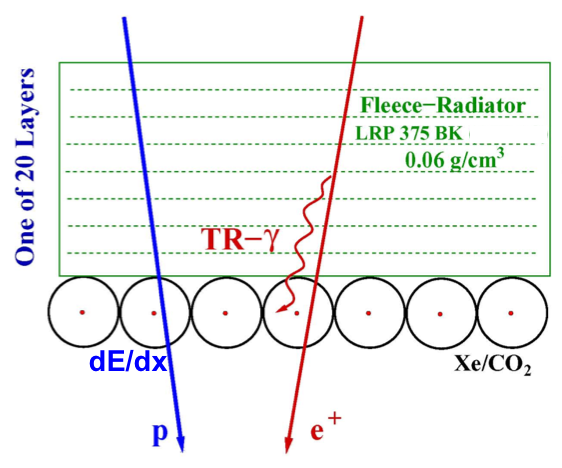
\includegraphics[width=0.47\columnwidth, height=0.28\textheight]{Figures/chapter3/TRD/TRDdEdX1.png} 
\label{TRDdEdXPlot}
}    
\subfigure[] { 
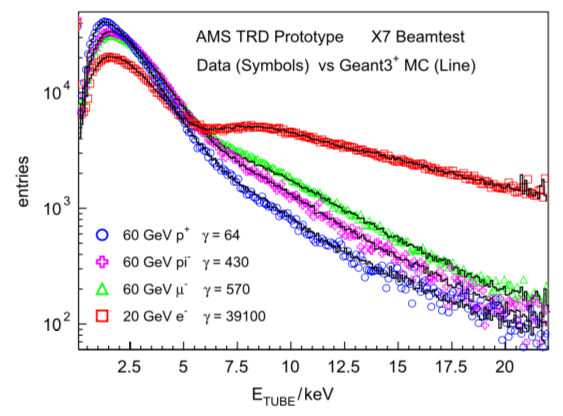
\includegraphics[width=0.47\columnwidth, height=0.25\textheight]{Figures/chapter3/TRD/TRDdEdX2.png}    
\label{TRDTubeEnergy}
}     
\caption[Illustration of the TRD separation between electrons and protons.]{Illustration of the TRD separation between electrons and protons: a) the transition radiation emitted by a positron while the proton can only produces the ${\rm{d}}E/{\rm{d}}X$ signals in the TRD \cite{AMSWebside}; b) the energy distributions measured by TRD straw tubes for 60 GeV protons, pions, muons and 20 GeV electrons during a beam test at CERN \cite{TRD_DEDXPaper}. }
\label{TRDdEdX} 
\end{figure}








  

\section{Silicon Tracker}

%%%% Magnet
To measure the rigidity and its sign, the AMS-02 detector is equipped with a silicon tracker and a magnet.
%Originally the magnet was a superconducting magnet with a 0.8 T magnetic field \cite{AMS02OriginalMagnet}. But due to the thermal issue and lifetime of the experiment, the superconducting magnet was replaced by a permanent magnet \cite{AMSPermanentMagnet}. 
The magnet used in the AMS-02 experiment is a permanent magnet with a 0.14 T magnetic field. The magnet has 64 Nd-Fe-B sectors arranged in a cylindrical shaped structure with a height of 0.8 m and an inner diameter of 1.1 m. The produced magnetic field is almost linear, and the magnetic field direction is defined as the X direction, the vertical direction is the Z direction, so the particle bending plane is the YZ plane. Outside the magnet, the leaking magnetic field is negligible so that the design can minimize the effect of the Earth’s magnetic field on the ISS. In figure \ref{MagnetTest}, the permanent magnet used in AMS-02 is shown. 
%Since the magnet is the same as AMS-01, the magnetic field of the magnet was remeasured again in 2010. Compared with the first measurement in 1997, the remeasurement shows the deviation is less than 1\% \cite{AMSWebside}.     %as showed in \ref{MagnetDeviation}.  

\begin{figure}[htpb]
\centering
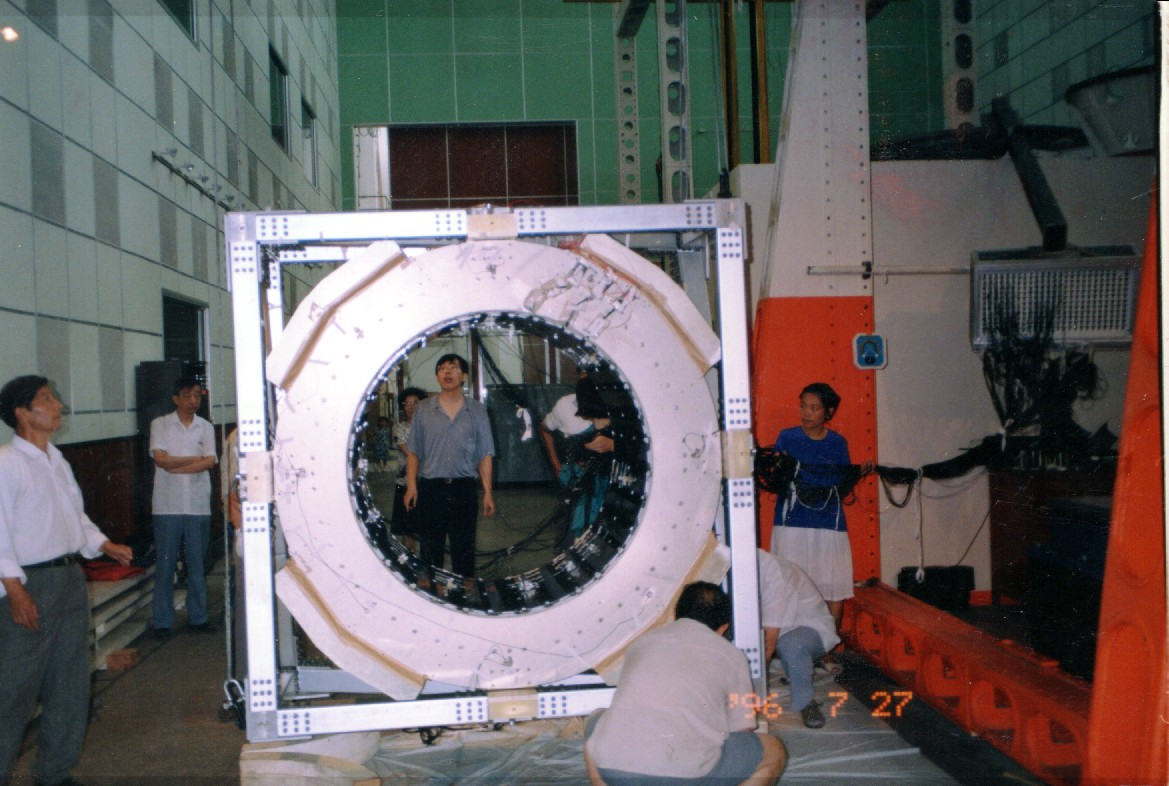
\includegraphics[width=0.8\textwidth, height=0.42\textheight ]{Figures/chapter3/Magnet/MagnetTest.jpg}
\caption[Preparing for test of the permanent magnet.]{Preparing for test of the permanent magnet in China Academy of Launch Vehicle Technology (CALT) \cite{AMSWebside}.}
\label{MagnetTest}
\end{figure}

%\begin{figure}[H]
%\centering
%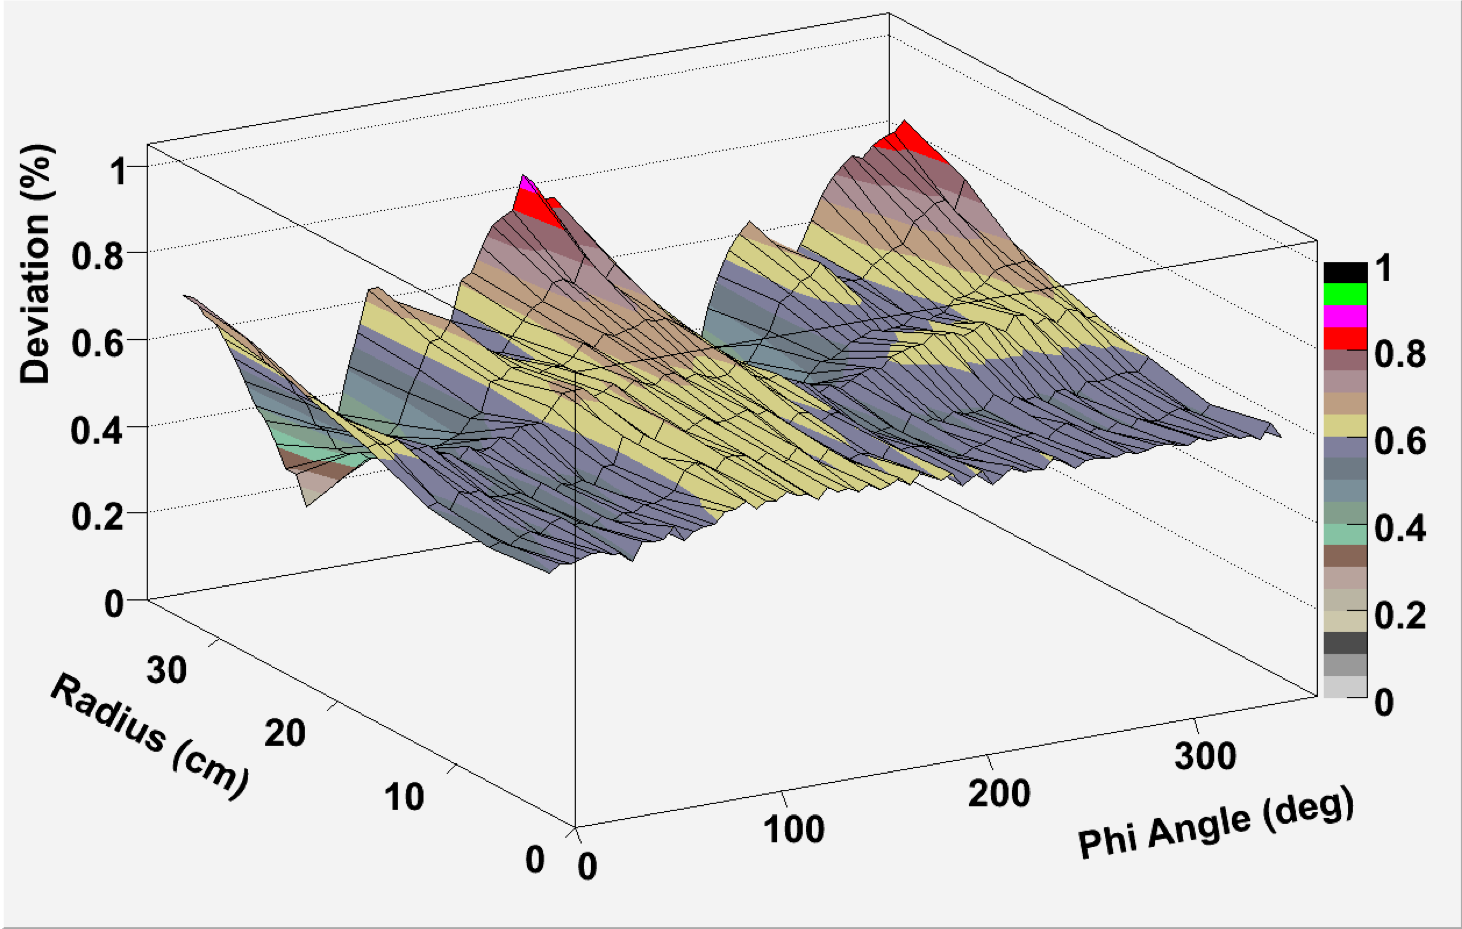
\includegraphics[width=0.8\textwidth, height=0.42\textheight ]{Figures/chapter3/Magnet/MagnetMeasurement.png}
%\caption{Deviation of the measured magnetic fields of the permanent magnet between 1997 and 2010 \cite{AMSWebside}. }
%\label{MagnetDeviation}
%\end{figure}


%%%% Tracker: With the permanent magnet, the silicon tracker can measure the charge $Z$ and also the momentum $p$ of the particle. \par
\begin{figure}[hbpt]
\centering
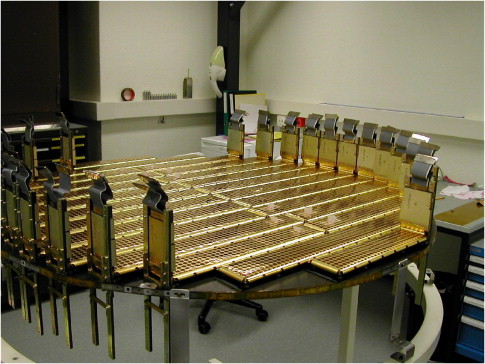
\includegraphics[width=0.8\textwidth, height=0.42\textheight ]{Figures/chapter3/Tracker/TrackerPlanePicture.jpg}
\caption[A silicon tracker inner plane fully equipped with ladders.]{A silicon tracker inner plane fully equipped with ladders \cite{TrackerPlanePicture}.}
\label{TrackerPlanePicture}
\end{figure}

%%%% Tracker Arrangement
The tracker of AMS-02 has nine silicon layers: the first layer is on the top of the TRD, the second layer is above the magnet and below the upper TOF, layers 3 to 8 are the so-called inner tracker layers as they are installed inside the permanent magnet and layer 9 is placed above the ECAL and below the RICH. In total, all nine layers have 2264 double-sided silicon micro-strip sensors. They are arranged into 192 ladders \cite{AMSTrackerPaper1, AMSTrackerPaper2}. The total active measurement area is 6.75 $m^2$. Each ladder has 1024 readout strips, 640 on the p-side and 384 on the n-side of the silicon sensors. So in total, there are 196608 readout channels. In figure \ref{TrackerPlanePicture}, a tracker inner plane equipped with ladders is shown.  \par 





%%%% Tracker Rigidity Measurement
Each double-sided silicon micro-strip sensor has a size of 41.360 $\times$ 72.045 $mm^2$ $\times$ 0.3 $mm$. When a particle goes through the sensor it creates electron-hole pairs in the middle. The created electrons drift toward the n-side and the holes toward the p-side. The X position measurement is obtained from the n-side and the Y position measurement is obtained from the p-side. Figure \ref{SiliconLayer} illustrates the process. The tracker's design results in spatial resolution of 10 $\rm{\mu m}$ and 30 $\rm{\mu m}$ in the bending and non-bending direction respectively for protons. Given the track hit positions, the rigidity and its sign can be reconstructed. By default, the rigidity is reconstructed with all the tracker layer hits. \par

\begin{figure}[htpb]
\centering
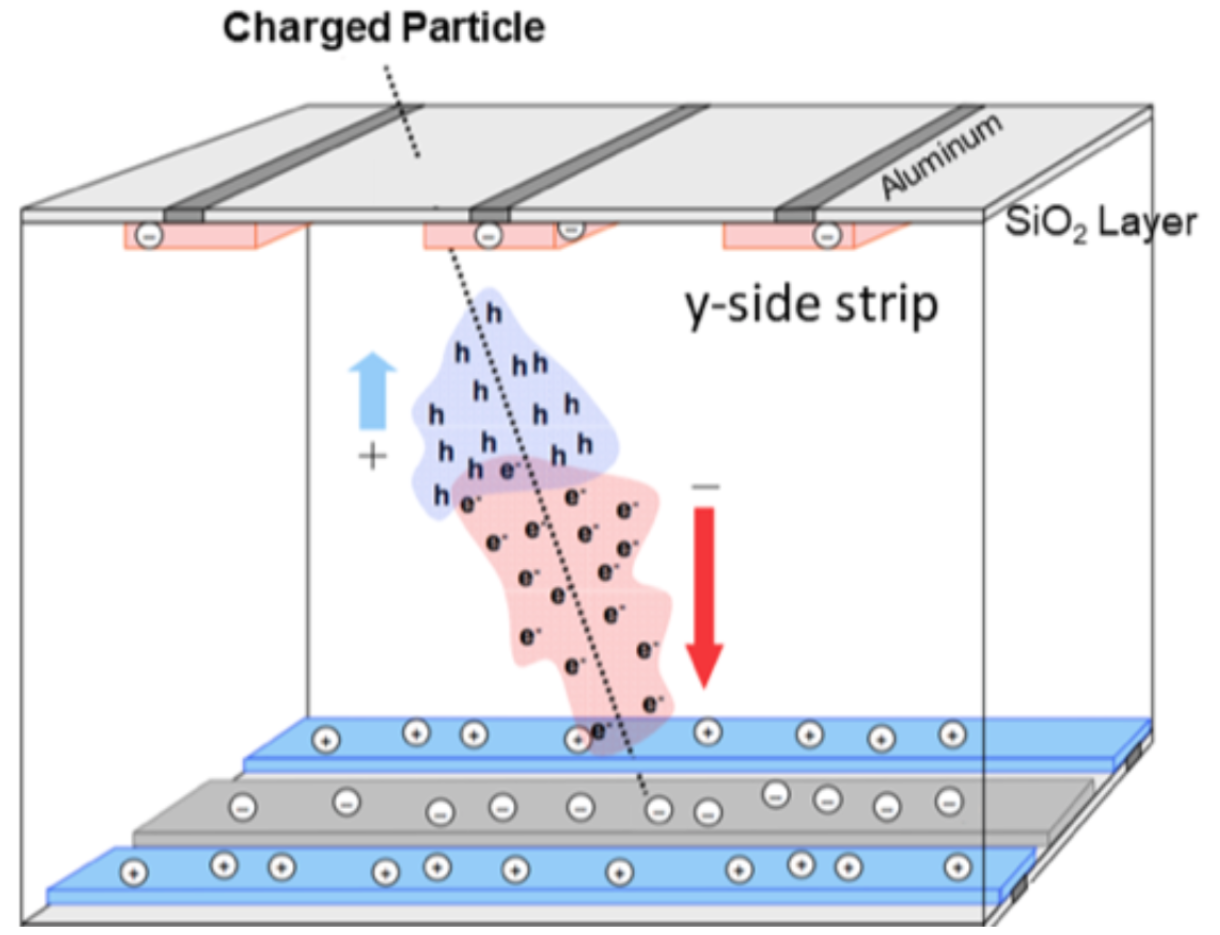
\includegraphics[width=0.8\textwidth, height=0.4\textheight ]{Figures/chapter3/Tracker/SiliconLayer.png}
\caption[Principle of operation of the double-sided silicon micro-strip sensors.]{Principle of the operation of the double-sided silicon micro-strip sensors. The electron-hole pairs produced by a charged particle drift towards the strips of the sensor as showing in this figure \cite{AMSWebside}.}
\label{SiliconLayer}
\end{figure}


%%%% Tracker Patterns
According to the presence of the tracker track hits in the different layers, various categories of tracker patterns can be defined. The tracker pattern definitions are given in table \ref{TackerPatterns}. In this table, $\checkmark$ denotes "have a hit associated to the track in this layer" and $\times$ denotes "does not have a hit associated to the track in this layer".
 
\begin{table}[h]
\center
\caption{Table of the tracker pattern definitions.}
\label{TackerPatterns}
\begin{tabular}{cccc} 
\hline
Tracker Pattern & Layer 1 & Layer 2 & Layer 9 \\
\hline
0  &  $\checkmark$   & $\checkmark$ or $\times$  & $\checkmark$   \\      %0  &  Layer 1 and 9, and maybe 2 \\
1  &  $\checkmark$   & $\checkmark$                     & $\times$            \\      %1  &  Layer 1 and 2, but not 9      \\
2  &  $\times$            & $\checkmark$                     & $\checkmark$   \\      %2  &  Layer 2 and 9, but not 1      \\
3  &  $\checkmark$   & $\times$                              &  $\times$           \\       %3  &  1 \\
4  &  $\times$            &  $\checkmark$                     &  $\times$           \\       %4  &  2 \\
5  &  $\times$           &  $\times$                              &    $\checkmark$  \\       %5  &  9 \\
-1 & $\times$            & $\times$                               & $\times$              \\       %-1 &  none \\
\hline
\end{tabular}
\end{table}


%%%% Tracker Charge Measurement
In addition, the deposited ionization energy ${\rm{d}}E/{\rm{d}}X$ is proportional to the square of the particle charge ($Z^2$). Therefore, the charge measurement in each layer can be obtained. The charge resolution of the inner tracker layers is $\Delta Z = 0.05$ for the charge of one particle.  \par



%%%% Tracker Calibration
The positions of the inner tracker layers are aligned and monitored by the Tracker Alignment System (TAS), which consists of 20 infrared laser beams that provides sub-micrometer position measurements \cite{AMSTrackerAlignment1, AMSTrackerAlignment2}. The positions of layers 1 and 9 are aligned with respect to the inner tracker by using cosmic rays over two-minute time windows. The resulting position accuracy is 5 $\rm{\mu m}$ for layer 1 and 6 $\rm{\mu m}$ for layer 9. \par 

%%%% Beam test
Before the launch of AMS-02, the whole detector was tested and calibrated at the CERN SPS  test beam facilities with 180 GeV and 400 GeV proton beams, as well as with positron, electron, and pion beams of 10 to 290 GeV. The tracker rigidity resolution function was determined with high precision and compared to MC simulation. Figure \ref{Calibration} shows the comparison between the tracker resolution measured at the 400 GeV proton beam and the one obtained by MC simulation. A good agreement between data and MC is observed.  \par

\begin{figure}[H]
\centering
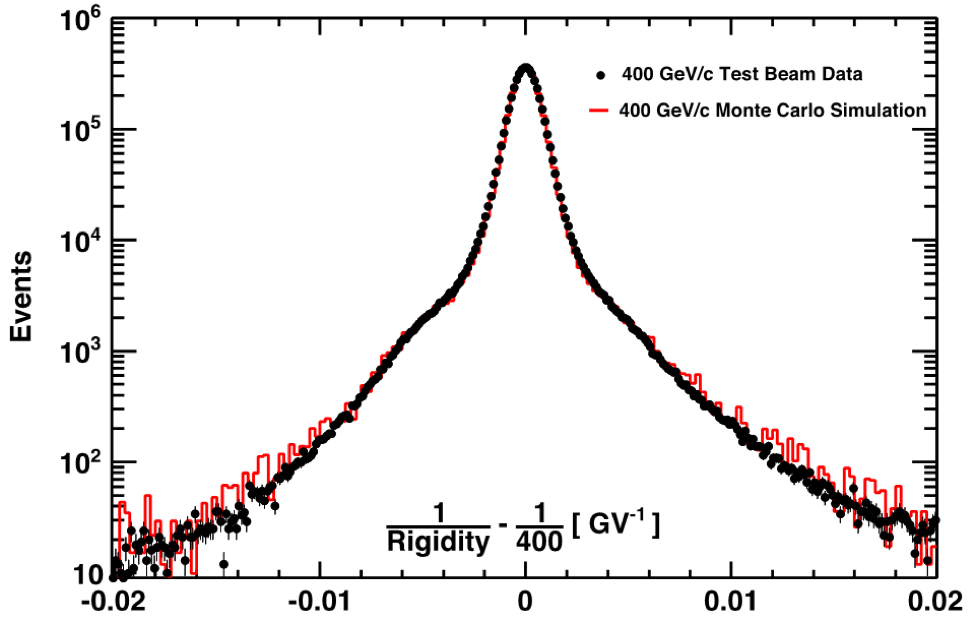
\includegraphics[width=0.8\textwidth, height=0.4\textheight ]{Figures/chapter3/Tracker/Calibration.png}
\caption[Tracker resolution measured with 400 GeV protons at the test beam and MC.]{Comparison between the tracker resolution measured with 400 GeV protons at the test beam and the MC simulation \cite{AMSWebside}.}  
\label{Calibration}
\end{figure}


%%%% Tracker Resolution 
Due to the resolution of the tracker and the multiple scattering \cite{TrackerResolutionPaper}, the resolution of the momentum measurement can be described by: 
 
\begin{equation}
\left(\frac{\sigma_{p}}{p} \right)^2 = \left( \sqrt{\frac{720}{N+4}} \frac{\sigma_{x} p  \sin \theta}{0.3 B L^2} \right)^2 + \left(\frac{0.2}{ \beta B \sqrt{LX_{0} \sin \theta} } \right)^2
\end{equation}

where $p$ is the momentum of the charged particle, $B$ is the magnetic field, $N$ is the equidistant measurements, $\theta$ is the track inclination angle, $L$ is the track length in the bending plane, $\sigma_x$ is the sagitta resolution in the bending plane, $\beta=\frac{v}{c}$, and $X_0$ is the radiation length of the traversed medium. \par 

\begin{figure}[htpb]
\centering
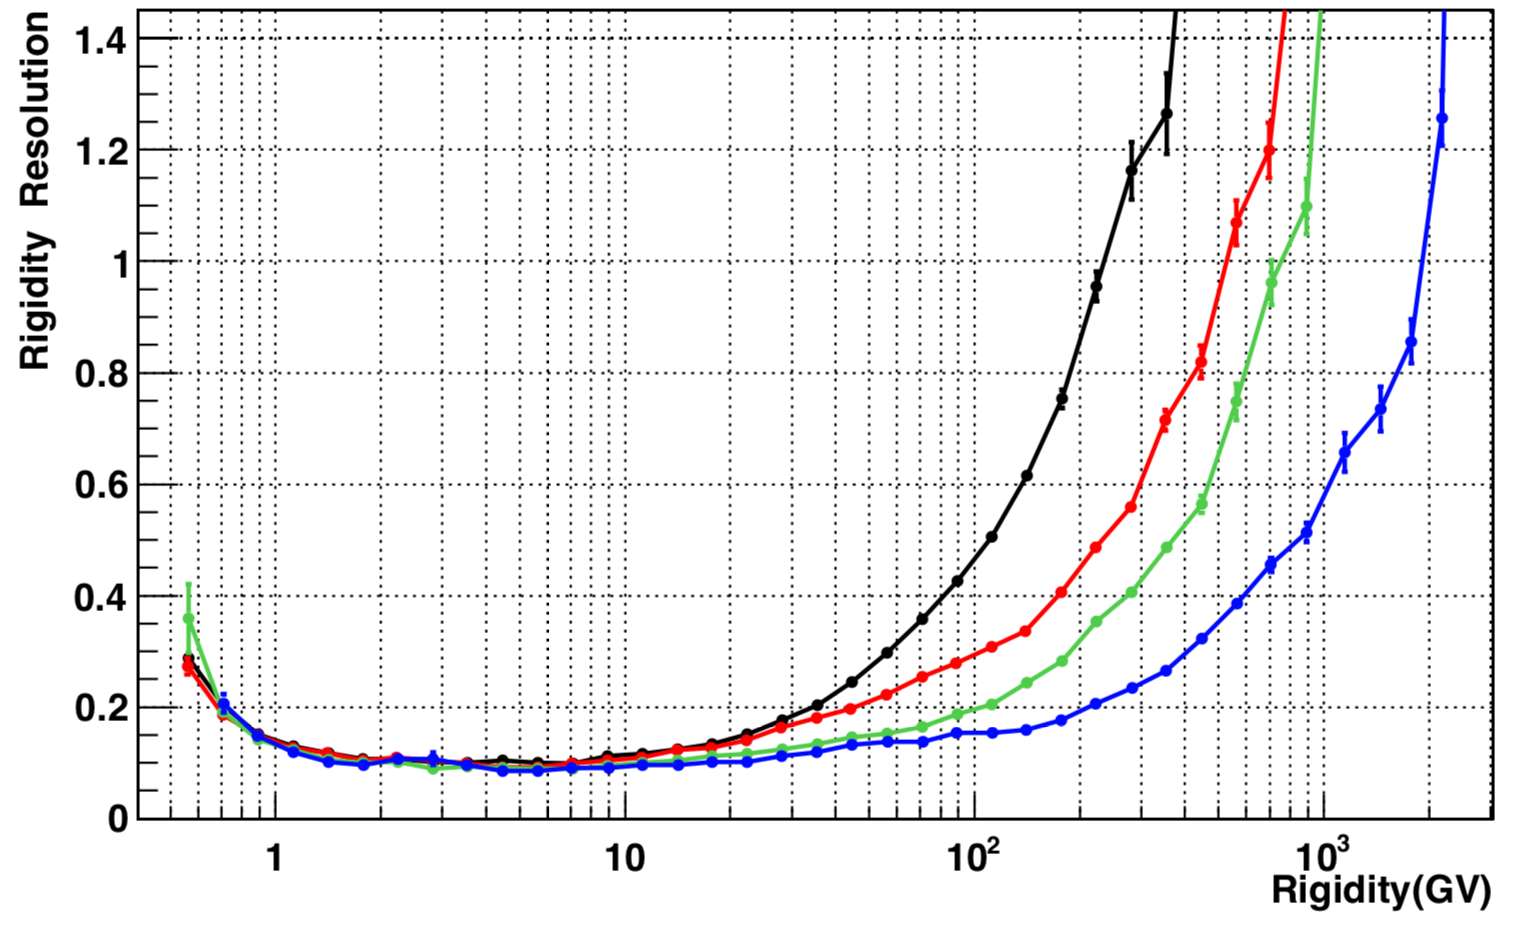
\includegraphics[width=0.9\textwidth, height=0.4\textheight ]{Figures/chapter3/Tracker/RigidityResolutionProton.png}
\caption[Tracker resolution from MC simulation for protons.]{The AMS-02 tracker resolution from MC simulation for protons \cite{ChargeConfusionReasonsAndTrackerResolutionPaper}. The four curves are for different tracker patterns: Black for inner tracker only, red for inner tracker plus layer 1, green for inner tracker plus layer 9 and blue for inner tracker plus layer 1 and 9. } 
\label{TrackerResolutions}
\end{figure}

In this equation, the momentum measurement equation consists of two terms. The first term describes the contribution of the tracker resolution and the second term the contribution of the multiple scattering. Since $R=pc/Ze$, the rigidity resolution is obtained. The AMS-02 tracker resolution has been studied extensively. In figure \ref{TrackerResolutions}, the AMS-02 simulated rigidity resolution for cosmic protons is shown. Below 1.5 GV, the rise is due to the multiple scattering, and the rise in the high rigidity range is mostly due to the detector’s resolution. The maximum detectable rigidity (MDR) is defined as the value of the rigidity $R$ where $\sigma_{R}=R$. This value is usually used to describe the highest rigidity that can be measured. For the AMS-02 tracker, the MDR for the protons in the full span (tracker pattern 0) is around 2 TV.



%\begin{figure}[h] 
%\centering   
%\subfigure[] {    
%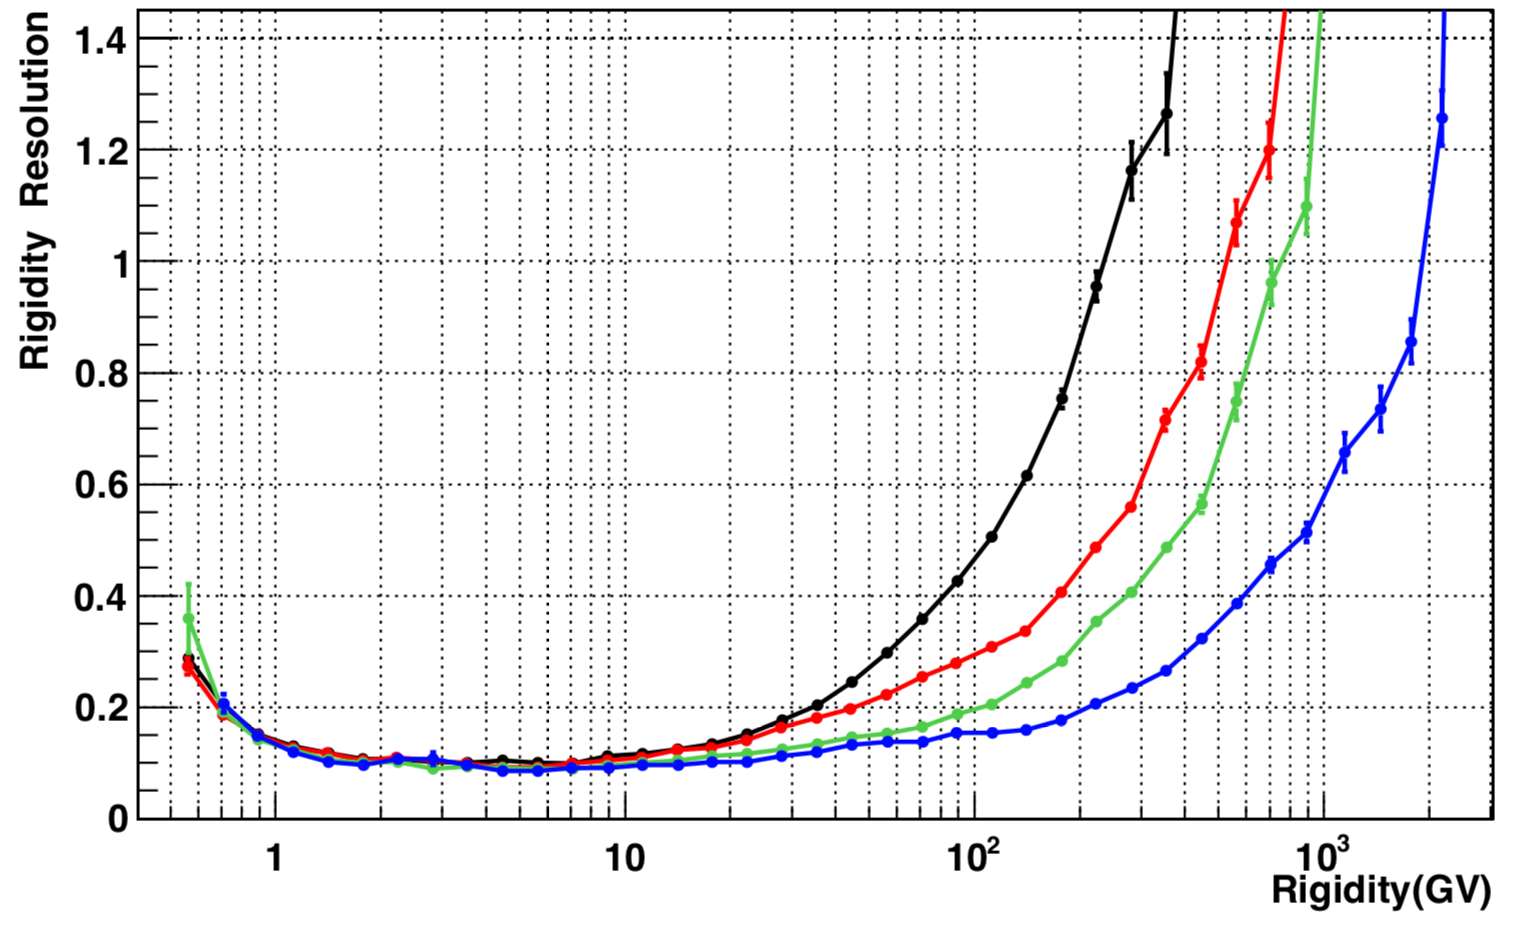
\includegraphics[width=0.45\columnwidth, height=0.225\textheight]{Figures/chapter3/Tracker/RigidityResolutionProton.png} 
%}    
%\subfigure[] { 
%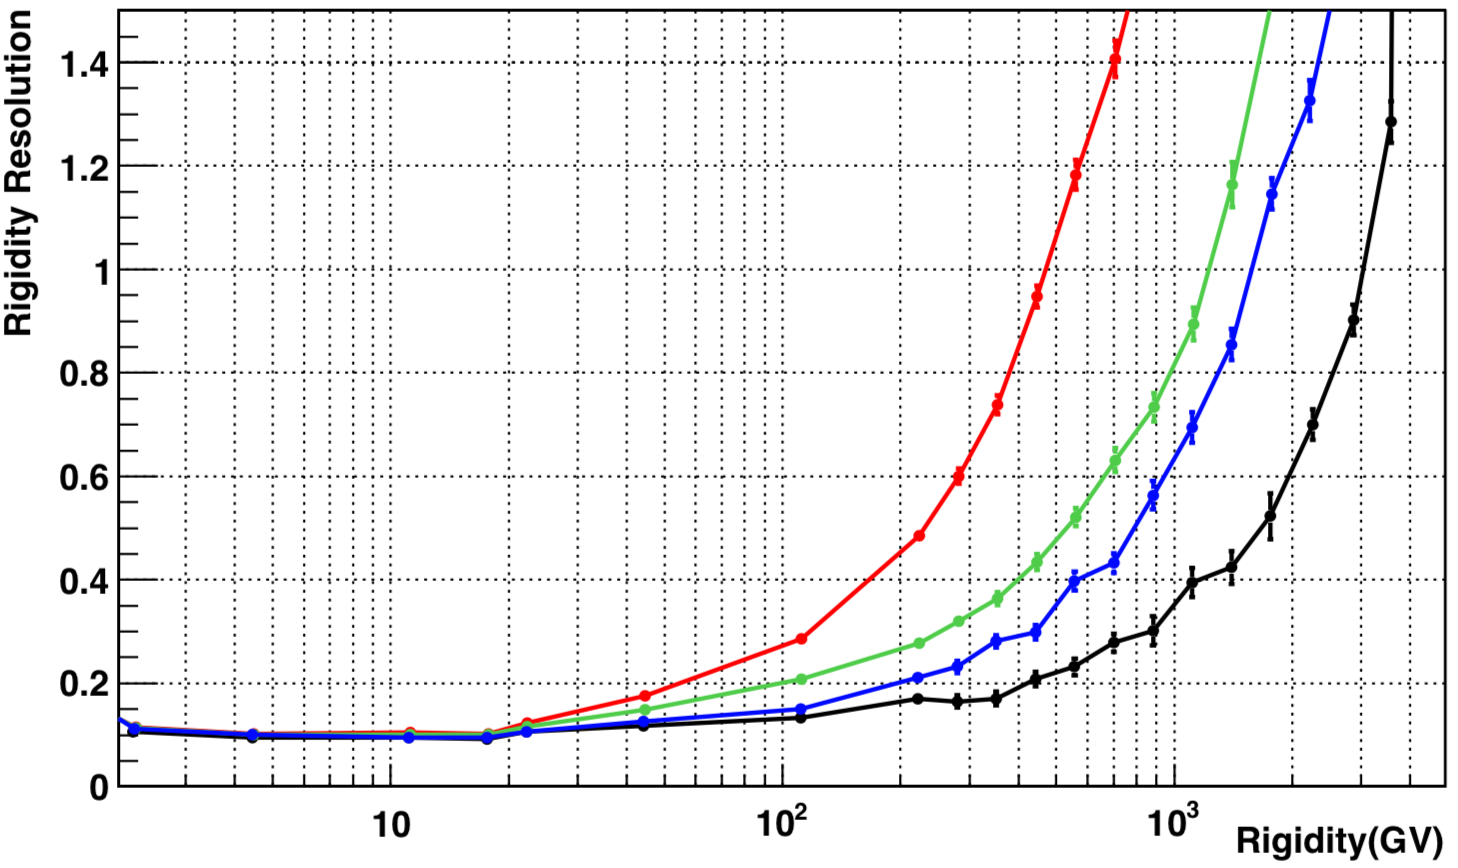
\includegraphics[width=0.45\columnwidth, height=0.225\textheight]{Figures/chapter3/Tracker/RigidityResolutionHelium.png}     
%}     
%\caption{Tracker resolution from MC simulation for a): proton and b): helium \cite{ChargeConfusionReasonsAndTrackerResolutionPaper}. The four curves are different tracker patterns: Black for inner tracker only, red for inner tracker plus layer 1, green for inner tracker plus layer 9, blue for inner tracker plus layer 1 and 9. } 
%\label{TrackerResolutions}    
%\end{figure}


%-----------------------------------------------------------------------------------------------------------------
%%%% TTCS off 
The heat produced by the electronics and radiators of the tracker can be removed by the Tracker Thermal Cooling System (TTCS). The TTCS is a two-phase $\rm{CO_2}$ cooling system with four cooling pumps. Due to aging and technique problems, the old four pumps were replaced by four new pumps in several spacewalks from November 2019 to January 2020.  




  
\section{Time Of Flight}

%  TOF
AMS-02 has four planes of TOF counters, plane 1 and 2 are above the magnet (Upper TOF), and plane 3 and 4 are below the magnet (Lower TOF) \cite{AMSTOFPaper1, AMSTOFPaper2}. Planes 1, 2, and 4 consist of eight plastic scintillator paddles, while plane 3 has ten paddles. The paddles have different lengths between 117 and 134 cm and a thickness of 1 cm. In the upper and lower TOF, the two planes are arranged in the X and Y directions as shown in figure \ref{TOFArrangement}. To avoid possible gaps between the paddles, the paddles are placed with a 0.5 cm overlapping. Each paddle is also equipped with 2 or 3 Photo-Multiplier Tubes (PMTs) on each end, which collect the light signal from the plastic scintillator and provide efficient particle detection.  \par
 
\begin{figure}[h]
\centering
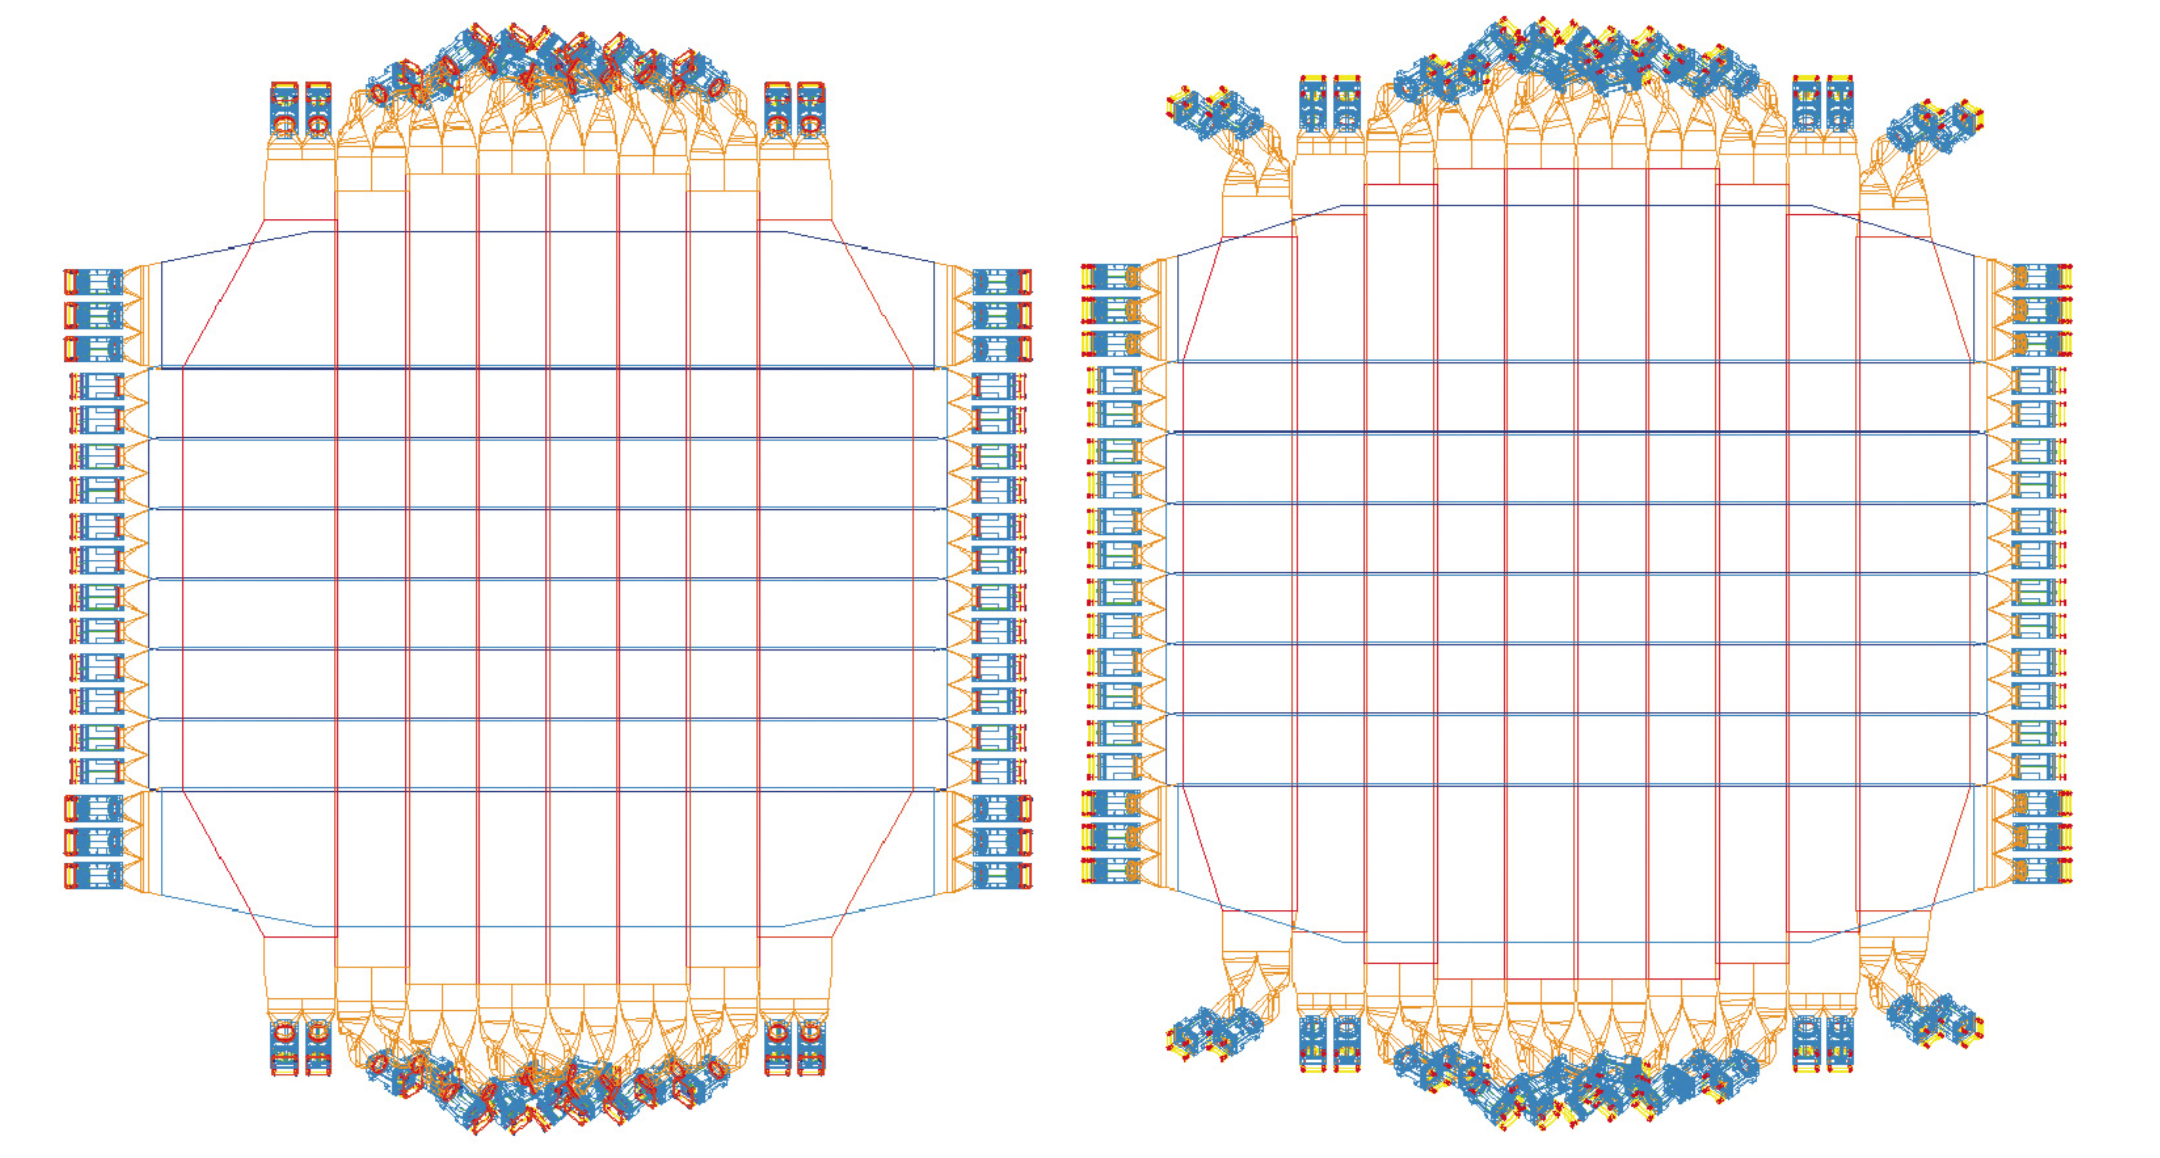
\includegraphics[width=0.8\textwidth, height=0.36\textheight ]{Figures/chapter3/TOF/Arrangement.png}
\caption[The TOF planes arrangement in the AMS-02 experiment.]{The TOF planes arrangement in the AMS-02 experiment. Left: Upper TOF and Right: Lower TOF \cite{TOFdetector}. }
\label{TOFArrangement}
\end{figure}

% TOF trigger
%Combining the information from all four planes, the TOF system can provide the particle trigger for the AMS-02 experiment. 
%More details on the trigger will be discussed in Section \ref{TriggerEfficiencySection}.  \par  

 % Time Resolution
The TOF system provides the particle's velocity by measuring the time difference between signals from the upper and lower TOF. Each counter's time resolution is around 160 ps, and the combined $\beta$ resolution is around $4 \%$ for $\beta \approx 1$ and $Z=1$ particles (figure \ref{TOFBetaResolution}). This provides the ability to discriminate between the up-going and down-going particles. Also, since the particle's mass is determined by: 

\begin{equation}
m=\frac{ZR}{\beta \gamma}
\label{MassEquation}
\end{equation}

combined with the rigidity measurement from tracker, the particle's mass can be obtained. \par  

%  Charge Resolution
Apart from measuring the velocity, the TOF can also provide the particle's charge. By measuring the ionization energy loss ${\rm{d}}E/{\rm{d}}X$, the charge of the particles can be independently obtained from the anode and dynode signals of the PMTs. The charge resolution is $\Delta Z=0.05$ for charge one particles (figure \ref{TOFChargeResolution}).  \par

\begin{figure}[H] 
\centering   
\subfigure[] { \label{TOFBetaResolution}    
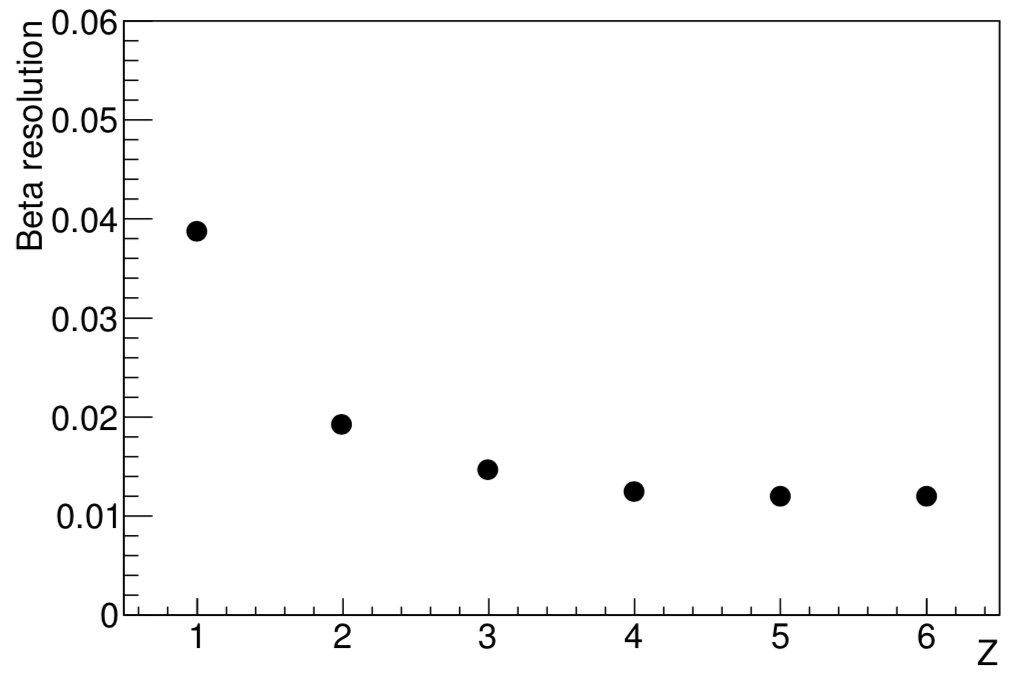
\includegraphics[width=0.45\columnwidth, height=0.225\textheight]{Figures/chapter3/TOF/TOFBetaResolution.png} 
}    
\subfigure[] { \label{TOFChargeResolution}    
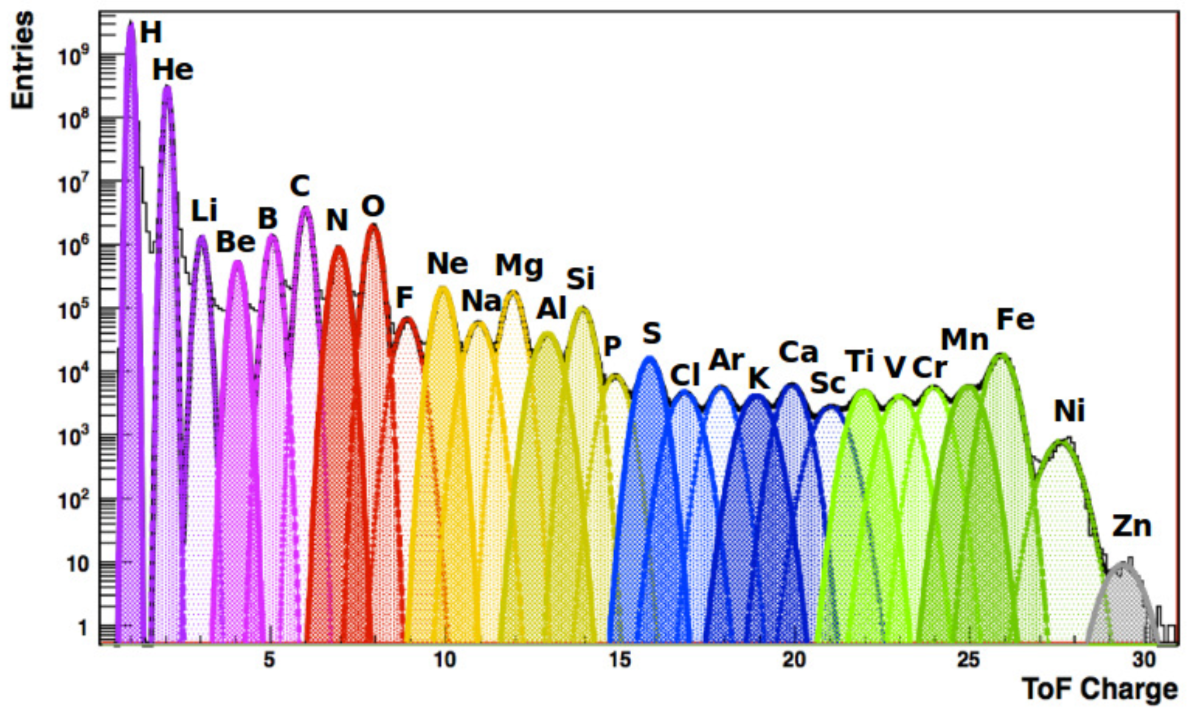
\includegraphics[width=0.45\columnwidth, height=0.225\textheight]{Figures/chapter3/TOF/TOFChargeResolution.png}    
}     
\caption[The TOF $\beta$ resolution and charge distribution.]{a) The TOF $\beta$ resolution as a function for particle charge \cite{TOFdetector}; b) The TOF charge distribution from protons (Z=1) up to Zinc (Z=30) \cite{TOFdetector}. }
\label{TOFReesolutions}    
\end{figure}

  

\section{Ring-Imaging Cherenkov Detector}

% AMS RICH
In the AMS-02 experiment, the RICH is installed below the lower TOF and above the ECAL. The RICH can measure the velocity and the charge of relativistic particles. It has two kinds of radiators at its top: a sodium fluoride (NaF) radiator in the center surrounded by a silica aerogel (Agl) radiator. Below the two radiators, there is an expansion volume in the middle and a PMT plane at the bottom \cite{AMSRICHPaper1, AMSRICHPaper2}. In figure \ref{RICHDetector}, the components of the RICH are shown. The whole RICH has the shape of a cone with an upper radius of 60 cm, a lower radius of 67 cm, and a height of 47 cm. \par

% Component: Radiators and beta measurement
When a charged particle traverses a dielectric radiator with a velocity greater than the velocity of light in this material, the particle emits a cone of Cherenkov photons. By measuring the emission opening angle of the Cherenkov radiation cone $\theta = \rm{arccos} (1/n\beta)$, the $\beta$ of the particle can be obtained. The RICH in the AMS-02 experiment has a radiator plane of two non-overlapping radiators. The central radiator consists of 16 NaF tiles with a size of 85 $mm \times$ 85 $mm \times$ 5 $mm$ each and a refractive index of n=1.33. Surrounding the NaF, there are 92 silica aerogel tiles with a size of 115 $mm \times$ 115 $mm \times$ 25 $mm$ each and a refractive index of n=1.05 \cite{AMSRICHPaper1}.    \par
 
\begin{figure}[htpb]
\centering
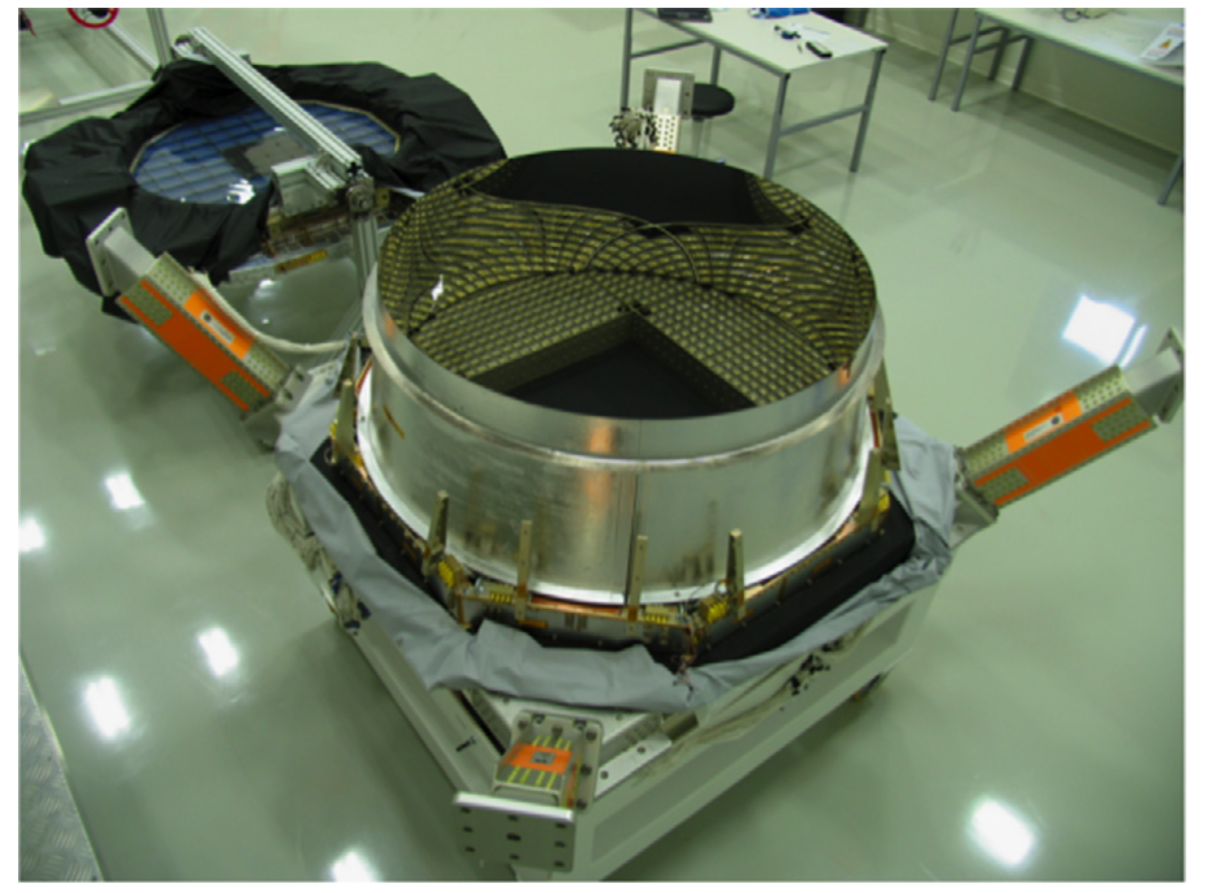
\includegraphics[width=0.8\textwidth, height=0.4\textheight ]{Figures/chapter3/RICH/RICHDetector.png}
\caption[The RICH PMT plane, its expansion volume and two radiators.]{The RICH PMT plane and its expansion volume at the front of the picture and the two radiators in the background \cite{RICHDetector}.}
\label{RICHDetector}
\end{figure}

Since $\beta=v/c$ and $n=c/v$, this leads to the requirement that particles which pass through the NaF radiator should have a velocity $\beta > 0.75$ in order to be detected, while those which pass through the Agl radiator should have a velocity $\beta > 0.953$.  \par

% Component: Expansion volume and PMT plane
\begin{figure}[H] 
\centering   
\subfigure[] { 
\label{RICHBetaResolution}    
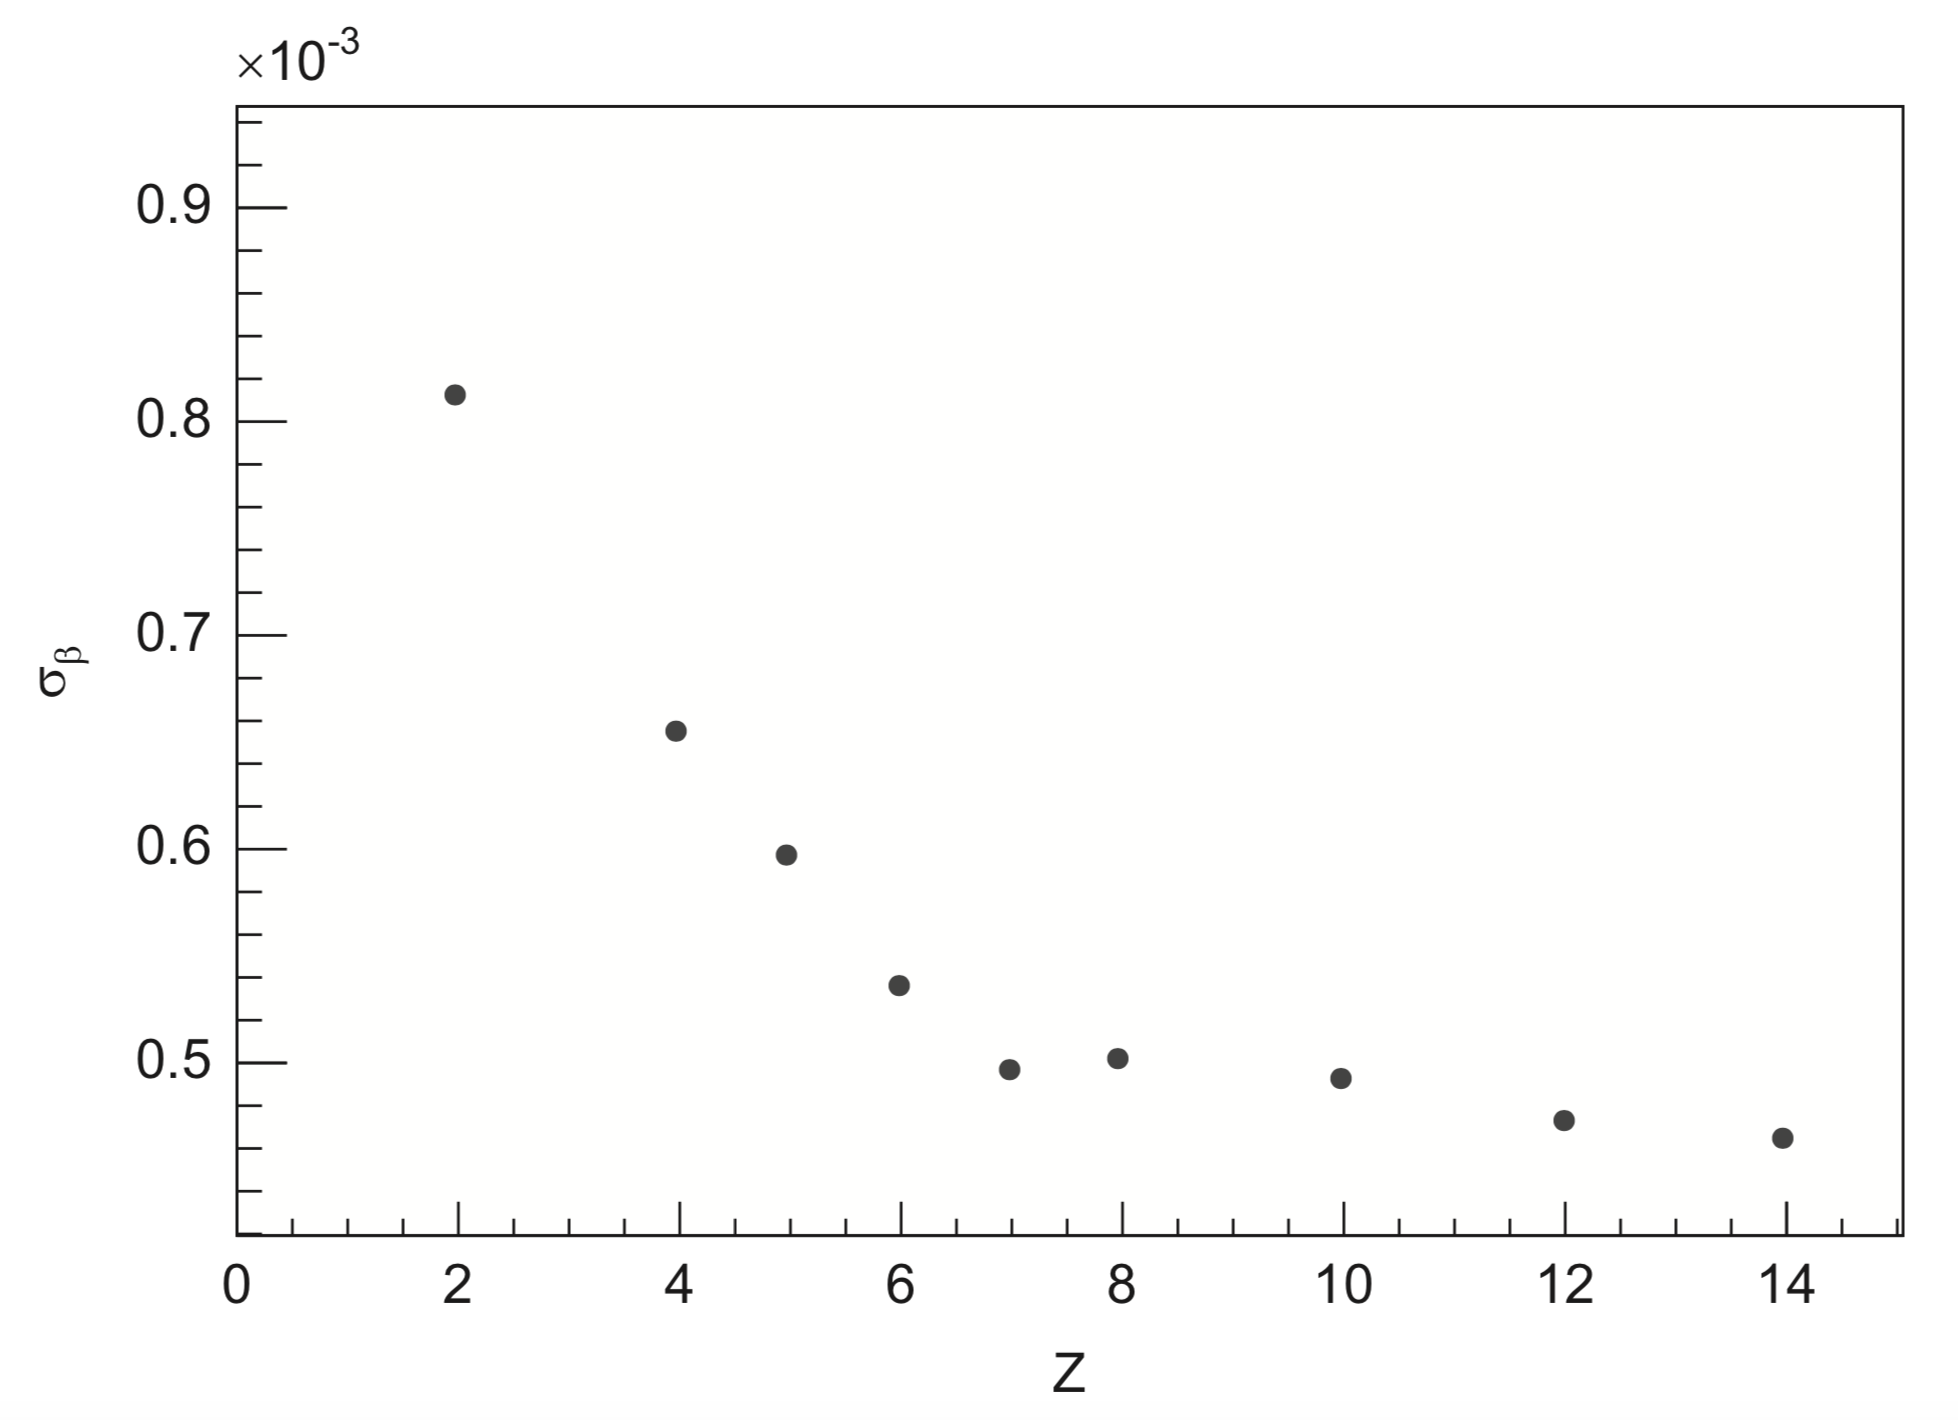
\includegraphics[width=0.45\columnwidth]{Figures/chapter3/RICH/BetaResolution.png} 
}    
\subfigure[] { 
\label{RICHChargeResolution}    
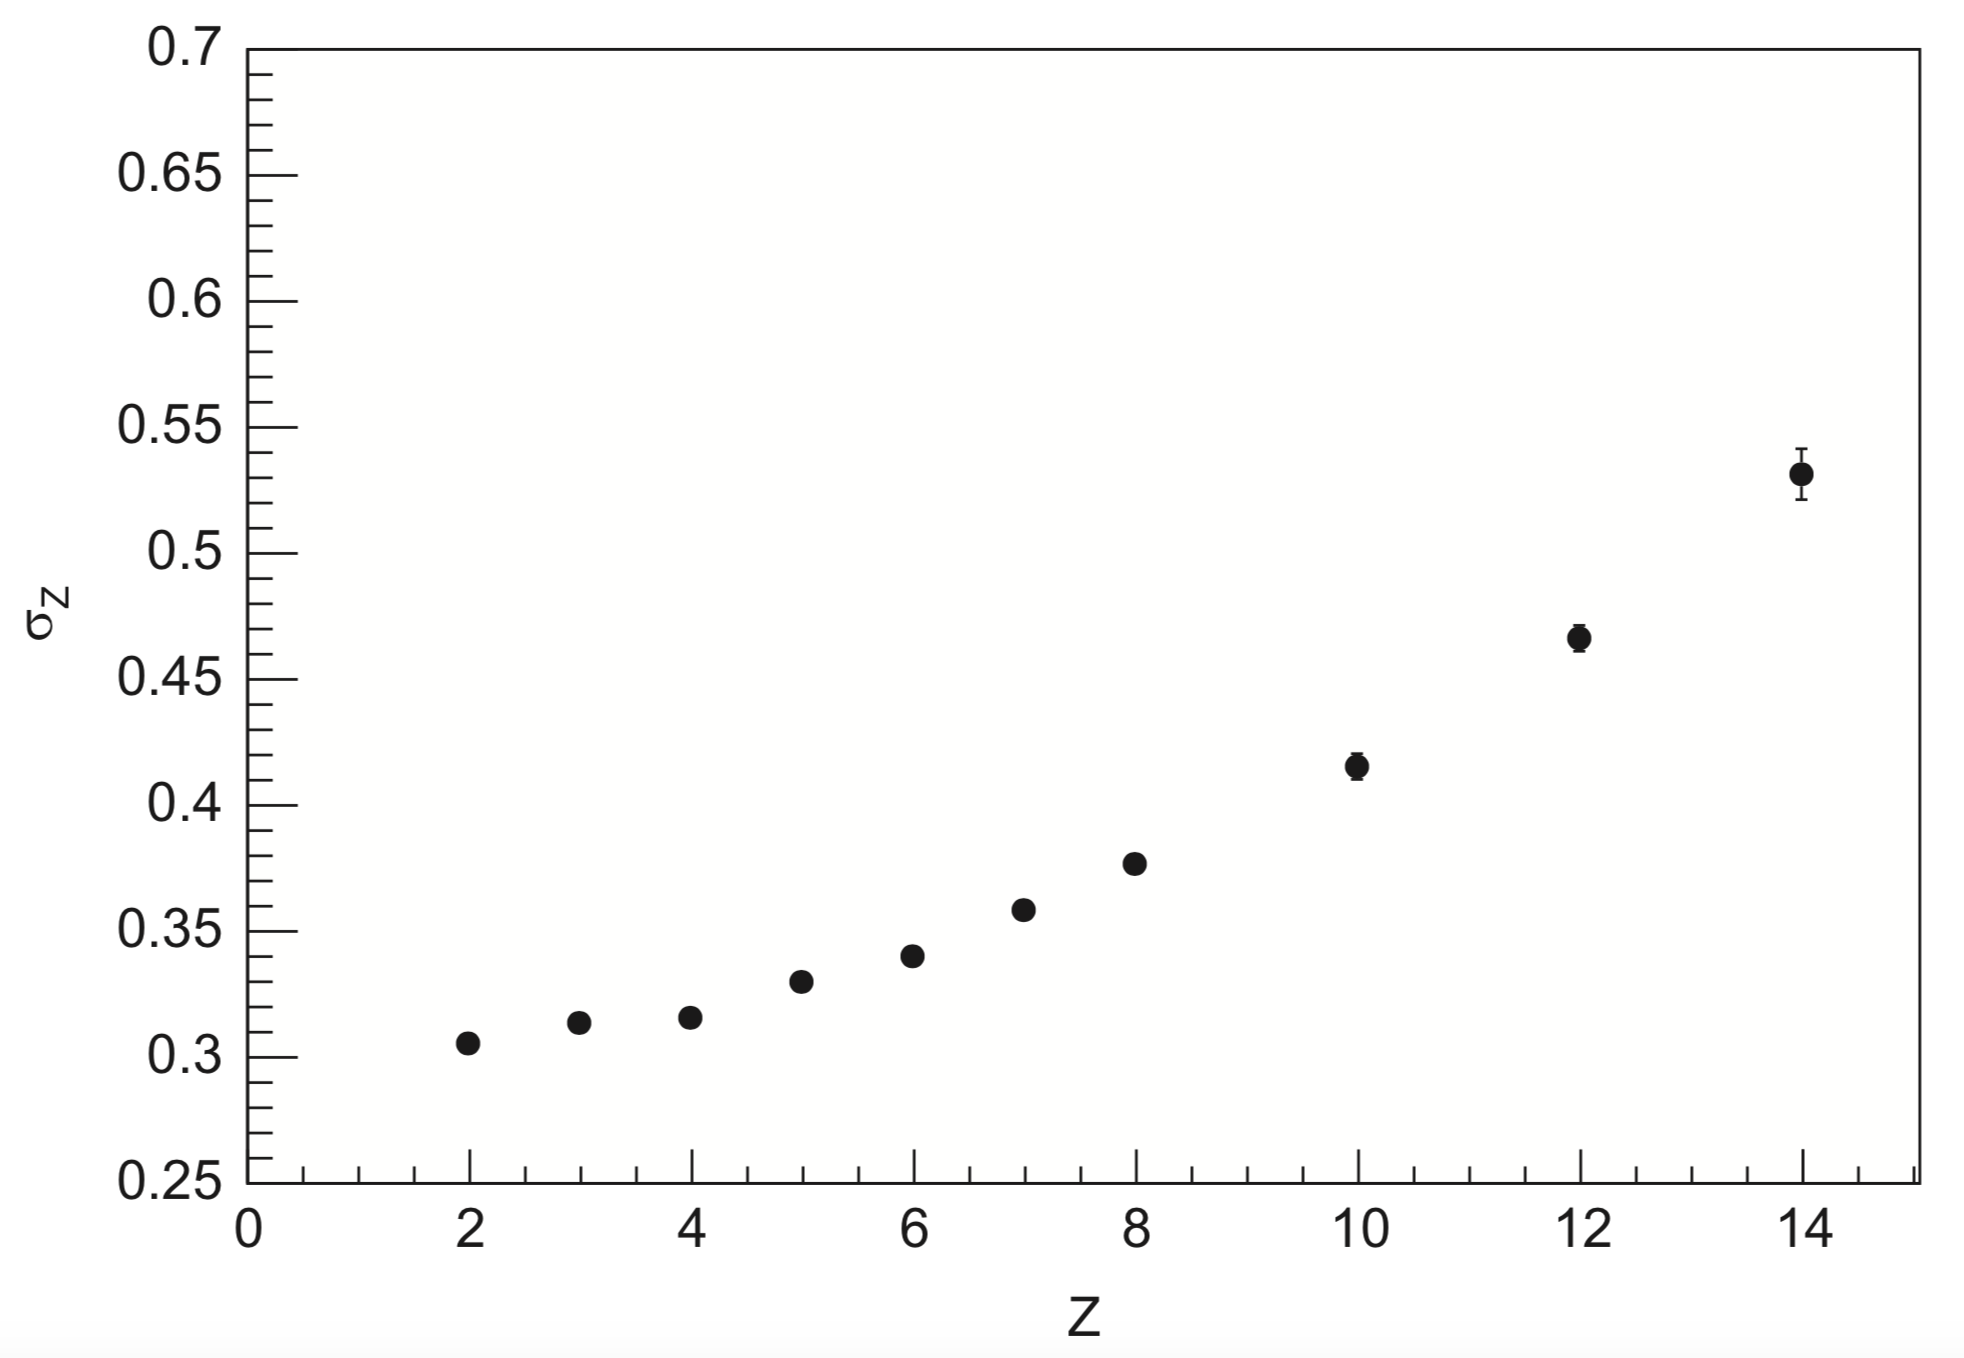
\includegraphics[width=0.45\columnwidth]{Figures/chapter3/RICH/ChargeResolution.png}    
}    
\caption[The RICH $\beta$ and charge resolution.]{a) The RICH $\beta$ resolution as a function of particle charge for the aerogel radiator \cite{RichResolution}; b) the RICH charge resolution as a function of particle charge \cite{RichResolution}.}
\end{figure}

A highly reflective mirror surrounds the expansion volume to increase the detection efficiency. The PMT detection plane at the bottom is equipped with 680 PMTs of $4 \times 4$ multi anodes. These PMTs detect the Cherenkov photons emitted in the radiators, and the effective spatial granularity is 8.5 $mm \times$ 8.5 $mm$. Since the sum of the signal amplitudes is proportional to $Z^2$, the charge of the particle can also be measured.   \par
      
% Resolutions: velocity and charge    

The velocity resolution of RICH is $\sim 10^{-3}$ for charge one particles for the aerogel radiator (figure \ref{RICHBetaResolution}). The charge measurement of RICH provides a resolution better than 0.5 for particles of charge up to 12 (figure \ref{RICHChargeResolution}).
% $\sigma_\beta / \beta \approx 10^{-3}$




  

\section{Electromagnetic Calorimeter}

% AMS Electromagnetic Calorimeter
The ECAL in the AMS-02 experiment can precisely measure the longitudinal and lateral electromagnetic shower development and also the deposited energy \cite{ECALPaper1, ECALPaper2}. It has a lead-scintillating fiber sandwich structure with an active area of 648 $mm$ $\times$ 648 $mm$, a thickness of 166.5 $\rm{mm}$ and a weight of $\sim 500$ kg. The ECAL has 98 lead foils and 50000 scintillating fibers in total. The entire structure corresponds to 17 radiation lengths ($X_0$). \par

% Super Layer
The ECAL consists of 9 superlayers with a thickness of 18.5 mm each. Each superlayer is made of 11 grooved lead foils alternated with ten fiber layers glued together with optical epoxy (figure \ref{ECALSuperLayer}) \cite{ECALFibres}, while the last foil of the last superlayer is made of aluminum. In each superlayer, the fibers are oriented along one direction only. By alternatively stacking the nine superlayers in the X and Y directions  (five superlayers in the X direction and four in the Y direction), the 3D image of the shower shape is obtained. Each superlayer’s fibers are read out by 36 PMTs at only one end. In total, the ECAL has 324 PMTs \cite{ECALPaper3}.   \par

\begin{figure}[h]
\centering
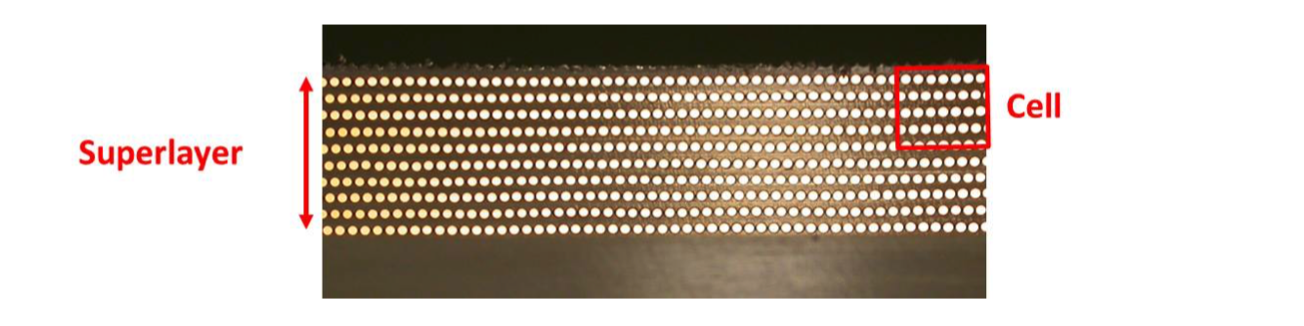
\includegraphics[width=1.0\textwidth, height=0.2\textheight ]{Figures/chapter3/ECAL/SuperLayer.png}
\caption[The ECAL superlayer structure.]{The ECAL superlayer structure. One cell is shown in red \cite{ECALPaper3}.}
\label{ECALSuperLayer}
\end{figure}

% ECAL Shower
When a particle goes through the ECAL, it interacts in an electromagnetic or hadronicdal way producing a shower \cite{ECALShowerPaper}. When an electron or positron traverses the ECAL, it emits photons by bremsstrahlung, then the emitted photons convert to electrons and positrons further by pair production, so a cascaded electromagnetic shower develops. While a proton or antiproton traverses the ECAL, it passes as a minimum ionizing particle (MIP) and leaves a relatively clear track. The produced hadronic shower primarily consists of pions and kaons which can interact or decay further. Due to the transverse momenta for massive secondaries and the possible production of neutral particles, the hadronic shower is wider and more irregular than the electromagnetic shower.  \par 

The different shower shapes can be used to distinguish between electrons and protons (antiprotons). Combined with the tracker measurement ($E/|R|$ cut), the ECAL provides a proton rejection power larger than $10^4$ at an electron efficiency of 90\% in the energy range of 3 to 1000 GeV. In figure \ref{ECALProtonRejectionPower}, the proton rejection of the ECAL is shown. \par


\begin{figure}[H] 
\centering   
\subfigure[] { \label{ECALProtonRejectionPower}    
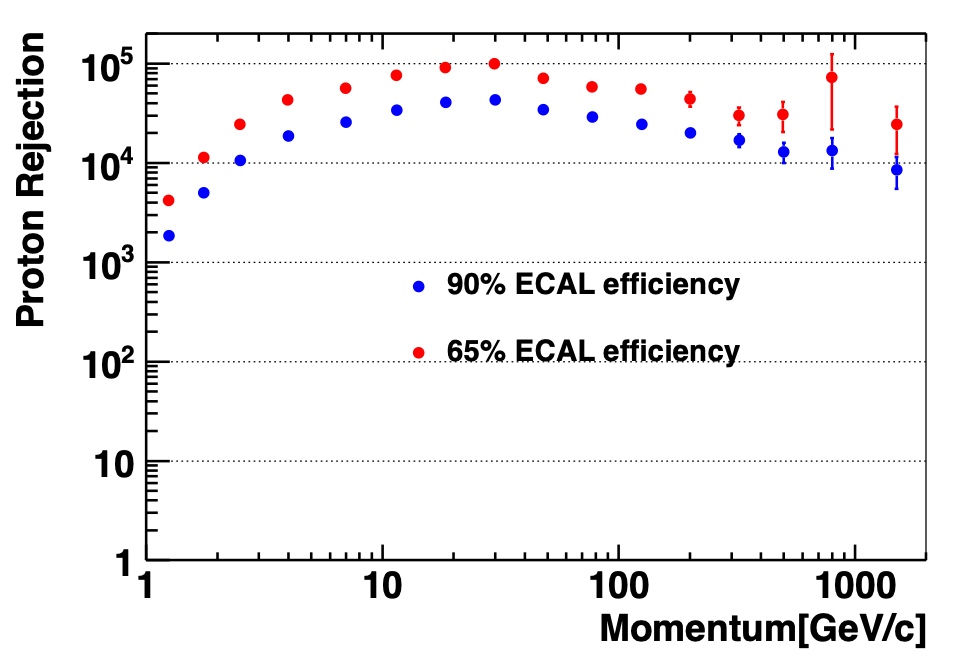
\includegraphics[width=0.45\columnwidth, height=0.225\textheight]{Figures/chapter3/ECAL/Ecal_Proton_Rejection.png} 
}    
\subfigure[] { \label{ECALEnergyResolution}    
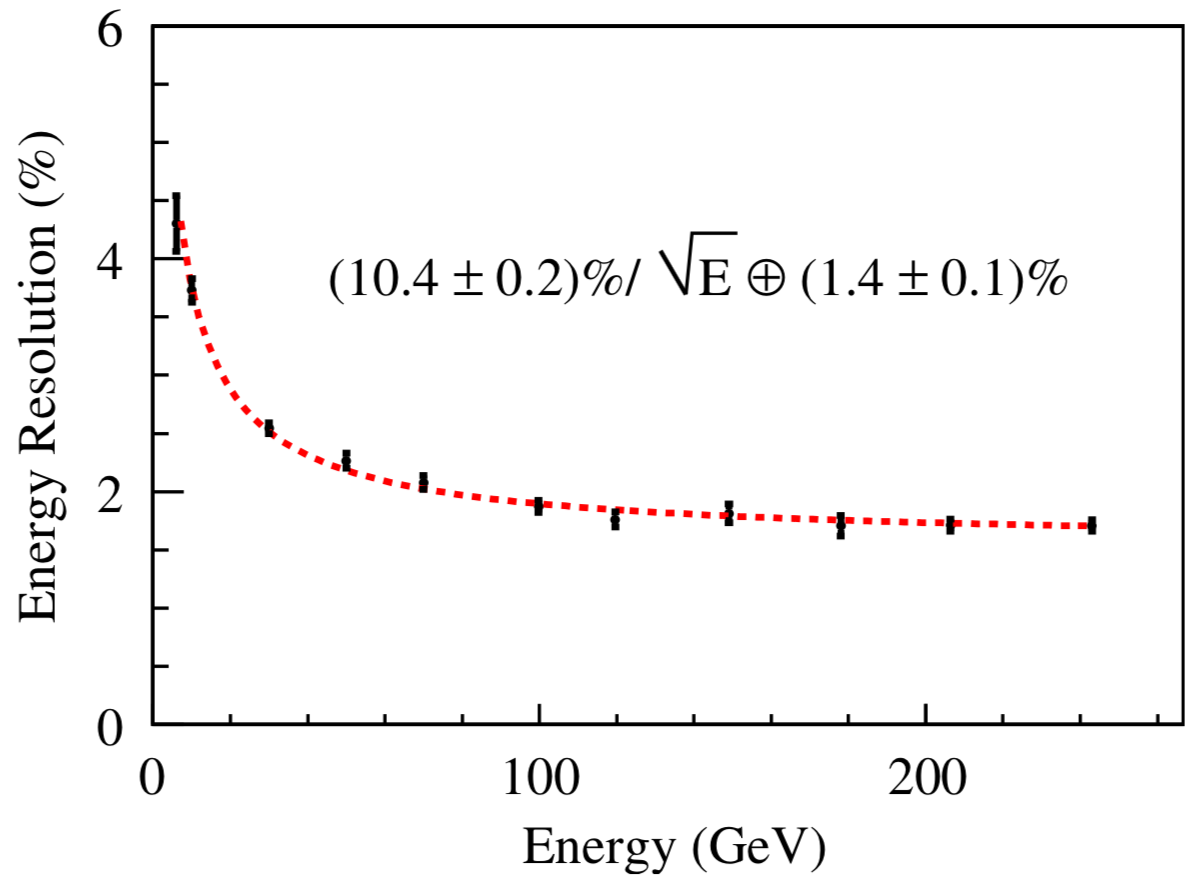
\includegraphics[width=0.45\columnwidth, height=0.225\textheight]{Figures/chapter3/ECAL/EnergyResolution.png}    
}     
\caption[The ECAL rejection power and energy resolution.]{a) The proton rejection of the ECAL at 65\% and 90\% electron efficiency \cite{AMSWebside}. b) The ECAL energy resolution determined from test beam data. The function of equation \ref{EcalResolutionEquation} is also shown (red dashed line) \cite{ECALResolution}.}
\end{figure}

% Resolution
The energy resolution has been determined in a CERN test beam \cite{ECALBeamTest} and can be described by \cite{ECALResolution}: 

\begin{equation}
\frac{\sigma (E)}{E} = \frac{(10.4 \pm 0.2) \%}{\sqrt{E(\mathrm{GeV})}}  \oplus (1.4 \pm 0.1) \%
\label{EcalResolutionEquation}
\end{equation}

Figure \ref{ECALEnergyResolution} shows the ECAL energy resolution measured in the test beam.


  

\section{Anti-Coincidence Counter}

% General description of ACC
The ACC in the AMS-02 experiment surrounds the inner tracker inside the magnet bore \cite{ACCPaper1, ACCPaper2} (figure \ref{ACCPicture}). Their purpose is to reject unwanted events with particles entering or leaving the inner tracker from the side. Moreover the ACC is used to reduce the trigger rate when the ISS is going through an area that is overwhelmingly dominant by low energy particle flux like the South Atlantic Anomaly (SAA) \cite{ACCAsTrigger}.  \par 

% Structure
The ACC has a cylinder shape of 1.1 m in diameter and 0.83 m in height. It is composed of 16 curved scintillator (Bicron BC-414) panels with 8 mm thickness, as shown in figure \ref{ACCScintillator}. When a particle traverses the ACC panels, it emits photons by ionization energy loss in the scintillators. Then the light is absorbed by the wavelength shifting fibres (WLS, Kuraray Y-11(200)M) that are embedded into the panels, and is transported to the PMTs (Hamamatsu R5946) placed on both ends of the ACC structure.  \par

\begin{figure}[h] 
\centering   
\subfigure[] { 
\label{ACCPicture}    
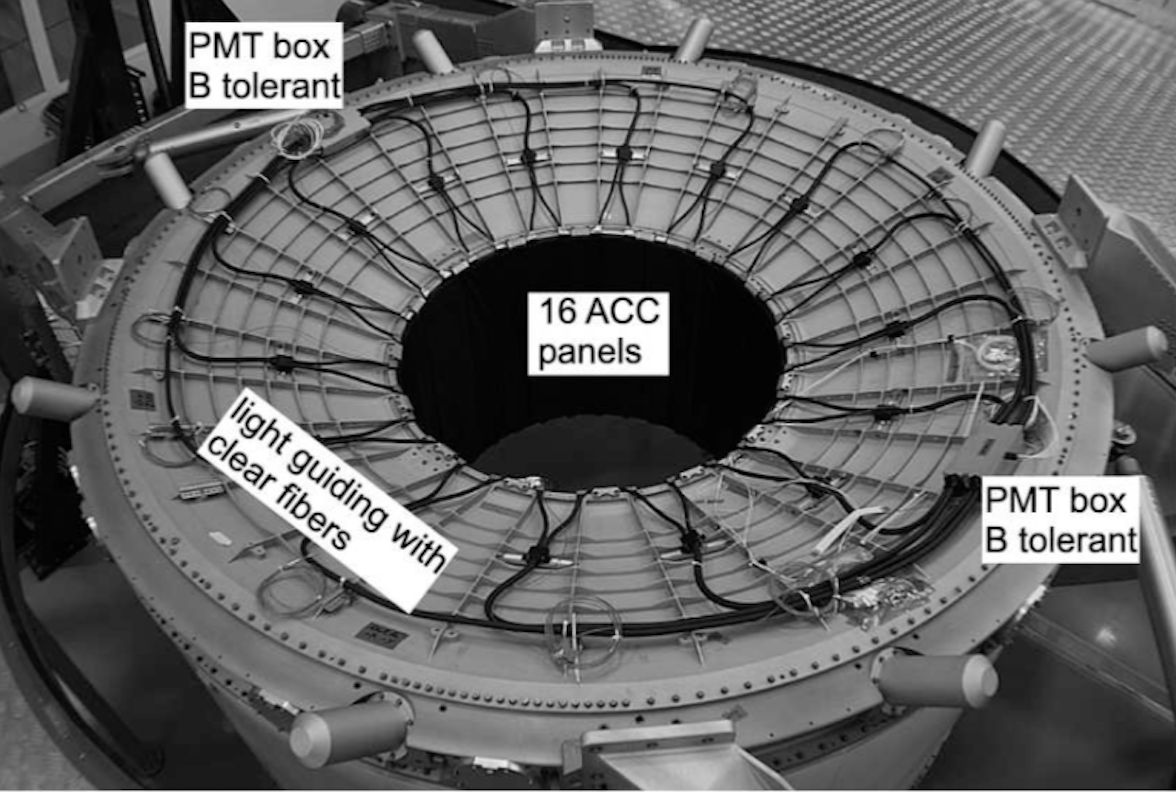
\includegraphics[width=0.52\columnwidth, height=0.29\textheight]{Figures/chapter3/ACC/UpperLeft.png} 
}    
\subfigure[] { 
\label{ACCScintillator}    
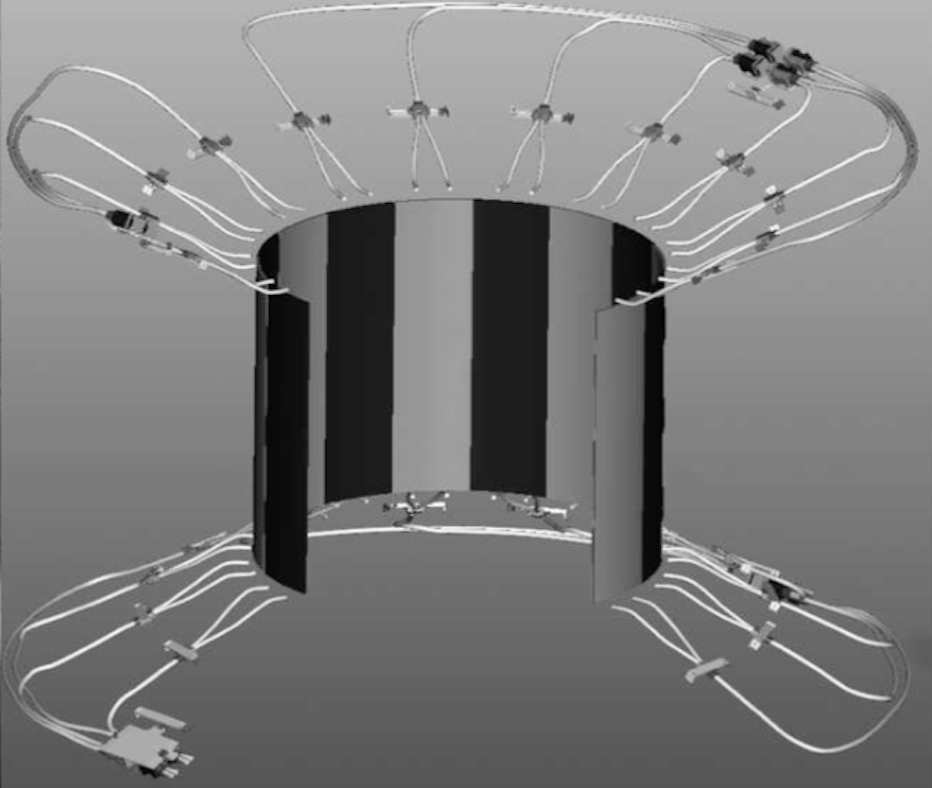
\includegraphics[width=0.40\columnwidth, height=0.29\textheight]{Figures/chapter3/ACC/UpperRight.png}    
\label{}
}    
\subfigure[] { 
\label{ACCFibers}    
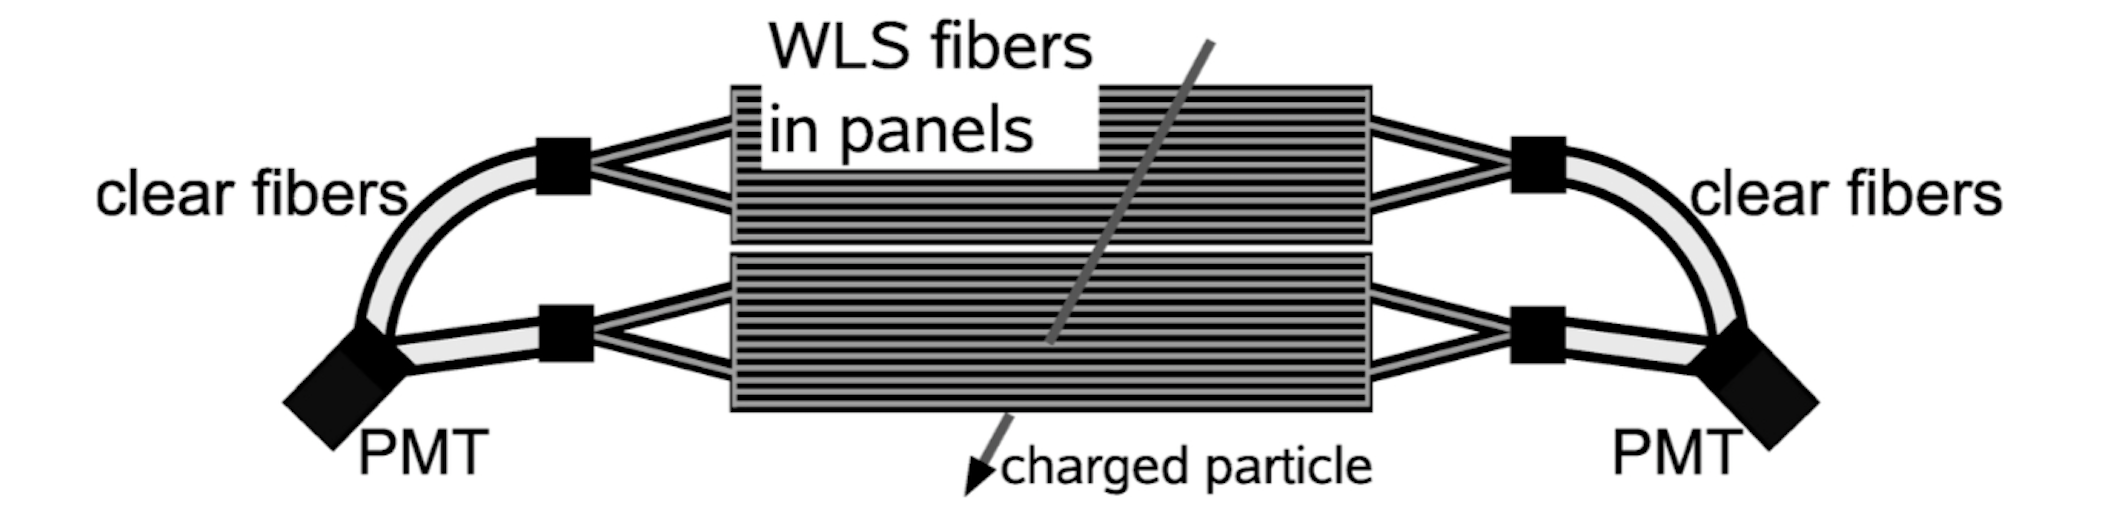
\includegraphics[width=1.0\columnwidth]{Figures/chapter3/ACC/Lower.png}    
\label{}
}    
\caption[The ACC scintillator panels pair and PMTs.]{a) The ACC system. b) The arrangement of the ACC scintillator panels. c) A panel pair and its connections to the PMTs \cite{ACCDetector}.}
\end{figure}

A pair of panels is connected to two same PMTs through clear fibers, as shown in figure \ref{ACCFibers}. This design provides redundancy capabilities and saves weight. The slot between these two panels has a tongue and a groove structure to minimize the detection inefficiency. The ACC panels efficiency has been measured at a muon test beam at CERN and found to be equal to 99.99\% \cite{AMSWebside}. \par

% Trigger
The ACC signals are used in the trigger logic to veto events with particles crossing from the side of the detector. Combined with the information from the TOF, the trigger is generated \cite{ACCAsTrigger}. 
%More details about the ACC's role in the trigger system will be given in Section \ref{TriggerEfficiencySection}.  


  




    
%%%% Chapter 4 %%%%

\chpt{Analysis} \label{ChapterAnalysis}


%% Flux definition 
In this chapter, the details of the antiproton analysis will be given, including all the steps of deriving the time-averaged and time-dependent antiproton to proton flux ratio. To determine the flux ratio, the definition of flux should be given first. In general, the flux as a function of true rigidity is calculated by: 

\begin{equation}
\label{FluxCalculationEquation}
\Phi(|R|_{\rm{true}}) = \frac{N(|R|_{\rm{true}})}{\Delta R \cdot T(|R|_{\rm{true}}) \cdot A(|R|_{\rm{true}}) \cdot \epsilon(|R|_{\rm{true}}) }
\end{equation}

where $N(|R|_{\rm{true}})$ is the number of events in this rigidity bin, $\Delta R$ is the rigidity bins width, $T(|R|_{\rm{true}})$ is the measuring time, $\epsilon(|R|_{\rm{true}})$ is the trigger efficiency and $A(|R|_{\rm{true}})$ is the effective acceptance. The quantities in equation \ref{FluxCalculationEquation} are as a function of true rigidity, while the number of events, derived from the template fit (a method to extract signal and background events from the total event distribution, see Section \ref{TempalteFitSection}), is expressed as a function of reconstructed rigidity. To get the event number in true rigidity, a procedure called "unfolding" is performed. This will be discussed further in section \ref{unfoldingsection}.  \par


%% Time Averaged: Antiproton to Proton flux ratio
In this thesis, the objective is the antiproton to proton flux ratio. Therefore, the dedicated formula should be determined based on the equation \ref{FluxCalculationEquation}. Given the antiproton and proton flux definitions:

\begin{equation} 
\begin{aligned}  
\Phi_{\bar{p}}(|R|_{\rm{true}}) =  \frac{N_{\bar{p}}(|R|_{\rm{true}})}{\Delta R_{\bar{p}} \cdot T_{\bar{p}}(|R|_{\rm{true}}) \cdot A_{\bar{p}}(|R|_{\rm{true}}) \cdot \epsilon_{\bar{p}}(|R|_{\rm{true}}) }\\
\Phi_{p}(|R|_{\rm{true}}) =  \frac{N_{p}(|R|_{\rm{true}})}{\Delta R_{p} \cdot T_{p}(|R|_{\rm{true}}) \cdot A_{p}(|R|_{\rm{true}}) \cdot \epsilon_{p}(|R|_{\rm{true}}) }
\end{aligned}
\end{equation}

the antiproton to proton flux ratio is defined as the antiproton flux divided by the proton flux. In this process, some terms can be strictly canceled out, like in the AMS-02 positron to electron flux ratio analysis \cite{ZimmermannPhDThesis}. Therefore, the overall calculation can be simplified:

\begin{equation} 
\begin{aligned}  
\frac{\Phi_{\bar{p}}(|R|_{\rm{true}})}{\Phi_{p}(|R|_{\rm{true}})} &= \frac{N_{\bar{p}}(|R|_{\rm{true}}) \cdot \Delta R_{p} \cdot T_{p}(|R|_{\rm{true}}) \cdot A_{p}(|R|_{\rm{true}}) \cdot \epsilon_{p}(|R|_{\rm{true}}) }{ N_{p}(|R|_{\rm{true}}) \cdot \Delta R_{\bar{p}} \cdot T_{\bar{p}}(|R|_{\rm{true}}) \cdot A_{\bar{p}}(|R|_{\rm{true}}) \cdot \epsilon_{\bar{p}}(|R|_{\rm{true}}) } \\ 
&= \frac{N_{\bar{p}}(|R|_{\rm{true}}) \cdot A_{p}(|R|_{\rm{true}})}{N_{p}(|R|_{\rm{true}}) \cdot A_{\bar{p}}(|R|_{\rm{true}})} \\ 
&= \frac{N_{\bar{p}}(|R|_{\rm{true}}) \cdot A^\mathrm{MC}_{p}(|R|_{\rm{true}}) \cdot (1+\delta_{p}(|R|_{\rm{true}}))}{N_{p}(|R|_{\rm{true}}) \cdot A^\mathrm{MC}_{\bar{p}}(|R|_{\rm{true}}) \cdot (1+\delta_{\bar{p}}(|R|_{\rm{true}}))} \\ 
& = \frac{N_{\bar{p}}(|R|_{\rm{true}}) \cdot A^\mathrm{MC}_{p}(|R|_{\rm{true}})}{N_{p}(|R|_{\rm{true}}) \cdot A^\mathrm{MC}_{\bar{p}}(|R|_{\rm{true}})}
\end{aligned}
\label{PbarOverProtonRatioEquation}
\end{equation}

where $A^{\mathrm{MC}}_{p}(|R|_{\rm{true}})$ and $A^{\mathrm{MC}}_{\bar{p}}(|R|_{\rm{true}})$ are the effective acceptances of proton and antiproton taken from the MC, $\delta_{p}(|R|_{\rm{true}})$ and $\delta_{\bar{p}}(|R|_{\rm{true}})$ are the data/MC corrections of the proton and antiproton effective acceptances, more details about these will be given in section \ref{EffectiveAcceptanceSection}. As shown in equation \ref{PbarOverProtonRatioEquation} the terms that cancel out in the antiproton to proton flux ratio are the rigidity bin width $\Delta R$, the measuring time $T(|R|_{\rm{true}})$, the trigger efficiency $\epsilon(|R|_{\rm{true}})$ and the data/MC corrections of the effective acceptance $(1+\delta(|R|_{\rm{true}}))$. The details of these terms will be shown in detail in the following sections. These cancellations simplify the calculation of the antiproton to proton flux ratio.  \par
% Although the measuring time and the trigger efficiency cancel out in the ratio calculation, they are still used in the unfolding process. 


%% Time Dependent: Antiproton to Proton flux ratio
For the time-dependent antiproton to proton flux ratio calculation, the formula in time bin $i$ is given in Equation \ref{TimeDependentPbarOverProtonRatioEquation}, which is similar to the time-averaged one. The difference is that the number of events is obtained from the individual template fits in every six Bartels Rotation time bin. \par

\begin{equation} 
\begin{aligned}  
\frac{\Phi_{\bar{p},i}(|R|_{\rm{true}})}{\Phi_{p,i}(|R|_{\rm{true}})} &= \frac{N_{\bar{p},i}(|R|_{\rm{true}}) \cdot \Delta R_{p,i} \cdot T_{p,i}(|R|_{\rm{true}}) \cdot A_{p,i}(|R|_{\rm{true}}) \cdot \epsilon_{p,i}(|R|_{\rm{true}}) }{ N_{p,i}(|R|_{\rm{true}}) \cdot \Delta R_{\bar{p},i} \cdot T_{\bar{p},i}(|R|_{\rm{true}}) \cdot A_{\bar{p},i}(|R|_{\rm{true}}) \cdot \epsilon_{\bar{p},i}(|R|_{\rm{true}}) } \\ 
& = \frac{N_{\bar{p},i}(|R|_{\rm{true}}) \cdot A^\mathrm{MC}_{p,i}(|R|_{\rm{true}})}{N_{p,i}(|R|_{\rm{true}}) \cdot A^\mathrm{MC}_{\bar{p,i}}(|R|_{\rm{true}})}
\end{aligned}
\label{TimeDependentPbarOverProtonRatioEquation}
\end{equation}


%% Content of Analysis Chapter
In section \ref{DataSelectionSection}, the cuts and selections are discussed. Section \ref{chargeconfusion} shows the construction of the charge confusion estimator. Section \ref{TRDEstimatorSection} describes how the TRD likelihood estimator is constructed. In section \ref{TempalteFitSection}, the template fit procedures to get the antiproton signals in different rigidity ranges are shown. Section \ref{EffectiveAcceptanceSection} gives the details about how to calculate the effective acceptances of antiproton and proton. In section \ref{MeasuringTimeSection}, the measuring time used in this analysis is determined. Although the measuring time is canceled in the antiproton to proton flux ratio calculation, it has to be calculated because the rigidity cutoff is not simulated in the MC simulation which is used for unfolding, also the measuring time in the time-dependent analysis is important to understand the event numbers change. Section \ref{unfoldingsection} shows the unfolding procedure. In section \ref{SecAntiprotonToProtonRatio}, the antiproton to proton flux ratio is given with statistical uncertainty only. In section \ref{SystematicUncertaintiesSection}, the different systematic uncertainties in different rigidity ranges are discussed.  \par

%In section \ref{TriggerEfficiencySection}, the trigger efficiency used in this analysis is calculated.
%In section \ref{SecAntiprotonToProtonRatio}, the formula for the calculation of antiproton to proton flux ratio is derived. 


\section{Data Selection} \label{DataSelectionSection}

% SubSection 1: General Description 
\subsection{AMS-02 Data and Monte Carlo Simulation}

%% ISS data
This section provides information on the data used in this analysis and presents the complete list of cuts and selections. In this analysis, the AMS-02 experiment data has been collected from May 20th 2011 to May 3rd 2021. Collected raw data need some calibration and alignment work and then can be reconstructed via the AMS-02 official software (named gbatch), resulting in the analysis data stored in ROOT files. The ROOT data analysis format is developed at CERN and it is dedicated for High energy particle physics analysis \cite{CERNROOTPaper}. Furthermore, a software package developed in Aachen called ACSoft is used to further process and store the data in a higher-level structure called ACQT \cite{BastianPhDPaper}. The analysis in this thesis is based on the so-called pass7 version of data (reconstructed via gbatch in version B1130). \par

%% Rigidity Bins 
The rigidity binning used in this analysis is the same as the one used in the previous AMS-02 proton analysis \cite{AMS02ProtonPaper}, which is determined by the rigidity resolution. At the rigidity regions higher than 80.5 GV, the rigidity bins are merged in every two bins to increase antiproton statistics.  \par

%% ISS data for Time Dependent Analysis  (Bartels Rotations)
%The sun is not a solid body but is made of gas plasma. Due to the solar rotations, different latitudes would show different rotation periods. From the view of the Earth, the solar rotations can be quantified with the Bartels Rotation Numbers. One Bartels Rotation Number is equal to exactly 27 days, close to the synodic rotation period \cite{BartelsRotationBook}. The counting of the Bartels Rotations started on February 8th 1832, a day that was arbitrarily assigned by Julius Bartels.   \par

For the time-dependent analysis, the collected ISS data is divided into six Bartels Rotations time bins. A Bartels Rotation is exactly 27 days, close to the synodic rotation period of the Sun. Because of the rigidity cutoff, the statistics in the low rigidity range in each time interval is limited. Therefore, the rigidity bins are also merged in every two original time-averaged rigidity bins in time-dependent antiproton analysis. The data collection used in this thesis started in May 2011, which corresponds to the Bartels Rotation 2426, and ended in May 2021, at the Bartels Rotation 2561. In total, the data can be divided into 23 intervals of six Bartels Rotations each though the last time bin has less data than the full six Bartels Rotations.  \par

%% TTCS 
Due to the upgrade of the cooling system of the AMS silicon tracker that took place from Nov 2019 to Jan 2020, the operation mode frequently changed during some periods as the cooling system pump had to be switched off. The data collected during these time periods is excluded and not used in this analysis. \par

%% MC data 
To validate the sub-detector's performance and study the detector's operation, an extensive set of MC simulations has been produced by the AMS-02 collaboration with the help of the Geant4 framework \cite{GEANT4Paper1, GEANT4Paper2}. The Geant4 is a software toolkit that simulates the passage of particles through matter. The interactions of the cosmic ray particles with all the AMS-02 sub-detectors and their support structure can be studied with this toolkit. By comparing the data distributions for different variables between MC and ISS data, the sub-detector's response to different cosmic rays can be systematically studied. \par   


%% comment: all the MC datasets used in this analysis. 
\begin{comment}  	

1. For CC training and CCProton Template:
B1042_pr.pl1.flux.l1a9.2016000_7.6_all
B1042_pr.pl1.flux.l1o9.2016000_7.6_all

2. For acceptance:
Proton:
B1042_pr.pl1.1800_7.6_all
Antiproton:
B1042_antipr.pl1.1800_7.6_all
B1220_antipr.pl1ph.021000.qgsp_bic_ams.plus10_7.8_all
B1220_antipr.pl1ph.021000.qgsp_bic_ams_7.8_all		
B1220_antipr.pl1ph.021000.qgsp_bic_ams.minus10_7.8_all	

3. Electron:
B1091_el.pl1.0_25_2000_7.6_all_merged	
B1091_el.pl1.0_25200_7.6_all		
B1091_el.pl1.2002000_7.6_all	

4. Data:
B1130_pass7	

others:	
B1220_pr.pl1ph.021000_7.8_all	
B1220_pr.pl1phpsa.0550.4_00_7.8_all	
B1220_pr.pl1phpsa.l19.5016000.4_00_7.8_merged 
B1220_pr.pl1phpsa.l1o9.flux.2016000.4_00_7.8_all
B1200_el.pl1.120_7.8_all	

\end{comment}		
	
%% MC data Usage: 1. CC estimator.  2. systematic error of acceptance 3. acceptance
%In this thesis, the MC datasets used are for protons, antiprotons, and electrons. 
In this thesis, the used MC datasets are:
\begin{itemize}
\item B1042 Protons MC with generated momentum from 20 to 16000 GeV
\item B1042 Protons MC with generated momentum from 1 to 800 GeV
\item B1042 Antiprotons MC with generated momentum from 1 to 800 GeV
\item B1220 Antiprotons MC with generated momentum from 0.2 to 1000 GeV 
\item B1091 Electrons MC with generated momentum from 0.25 to 200 GeV
\item B1091 Electrons MC with generated momentum from 200 to 2000 GeV
\end{itemize}

\begin{figure}[H]
\centering
\includegraphics[width=1.0\textwidth]{Figures/chapter4/DataSelection/{B1042_antipr.pl1.1800_7.6_all_mc_iss_ratio}.pdf}
\caption[The antiproton statistics comparison between MC and ISS data.]{The statistics comparison between antiproton numbers from MC simulation and antiproton events from ISS data. The jumps in the ISS data are due to the different selections in different rigidity ranges. The statistics of antiproton MC is at least ten times larger than the antiproton events from ISS data.}
\label{MCISSStatisticsCompare}
\end{figure}

%657: discuss the jumps in the spectral shapes

In figure \ref{MCISSStatisticsCompare}, the statistics of antiproton MC simulation and the antiproton events from the ISS data (which will be given in the following sections) are shown. The antiproton MC statistics is at least ten times larger than the antiproton events determined from the ISS data.        \par

Different MC datasets are generated in different momentum ranges for various purposes. For example, one of the main purposes of using MC proton data in this analysis is to study the proton charge confusion events, which are proton events but measured with the wrong rigidity sign. The reasons are finite tracker rigidity resolution and the interactions with the sub-detectors \cite{ChargeConfusionReasonsAndTrackerResolutionPaper}. By selecting the negative rigidity data samples from the proton MC dataset, the proton charge confusion events can be studied. This issue will be discussed in more detail in Section \ref{chargeconfusion}. The MC datasets are also used for other purposes like calculating effective acceptance and determining the systematic uncertainties due to acceptance, these will be shown in detail later in this chapter.    \par  

%% MC data reweighting
For the simulated MC events, the generated momentum spectrum does not perfectly match the real cosmic spectrum. This could introduce bias in some variable distributions in MC. In order to correct this, the weight of each event in a MC dataset has to be reassigned by making the flux computed from this MC dataset equal to a reference flux. For example, the AMS-02 published proton flux result \cite{AMS02ProtonPaper} is used as the reference flux for proton MC datasets. The acquired re-weighting factor will be used in filling variable histograms for further study.  \par  

%\begin{equation}
%w=\frac{\phi}{MC}
%\end{equation}

%Fabian:
% To correct this, a weight is determined for each event such that a flux computed from the MC events is equal to a reference flux. In this analysis, a model for the electron flux is used as a reference (Appendix A.2) and the protons are assumed to follow a power law with a spectral index of γ = −2.7 and solar modulation calculated according to the force field approximation (equation 2.4) with a potential of φ = 500 MV.
%Manbing:
% To get a realistic distribution of MC data, reweighting of each event is applied. This is done using the flux spectrum measured by AMS [14] as a scaler. Figure 4.5 presents the lithium MC event weights as a function of the true rigidity.
% With the weight factors, the MC rigidity spectrum has the same shape as the data sample.
%Mine_old:
%In order to correct this, the weights of MC events are reassigned by making the spectrum of MC simulation is same as the reference one. 


%% Introducing data selection
Up to May 2021, the AMS-02 experiment has collected more than 174 billion cosmic ray events. To select antiproton events from them, cuts and event selections are applied. There are two levels of selection; the first one is the so-called “Preselection” and the second one is the more refined “Selection”. In the next few subsections, the definition of all selections and their pass ratios will be given. The pass ratio is the event number passed in this cut to the total event number before applying the selector (a group of cuts at this level of selection) to which this cut belongs. \par 
%676: the "pass ratio" is not well defined. What exactly is the denominator? Events before all cuts? After the previous cut? ...?

%  SubSection 2. : Preselection
\subsection{Preselection Cuts}
The first level of cuts and selections is the preselection. The purpose is to discard data taken during bad sub-detectors operation conditions or have bad quality. These selections are general and applied before any cosmic ray component AMS-02 analyses. The preselection consists of two parts: data taking quality cuts and analysis data quality cuts. Each part is a selector. \par 

%% 2.1 Preselection: data taking quality cuts
Data taking quality cuts require all the sub-detectors running in nominal conditions, and the data taking conditions are normal. The first one excludes the period that any sub-detector operates under special conditions or undergoes testing. For example, the TRD gas refill procedure takes place once per month. In this period, the data taken is not included in this analysis. The second one requires that the data taking period is normal. For instance, if the ISS is in the SAA area, the data taken in this period is not included in this analysis. In summary, Table \ref{data taking quality cuts} shows the pass ratios of all the data taking quality cuts. \par
%The pass ratio is defined as the ratio of event numbers passed in this cut to the total event numbers before applying the cuts in the list.


\begin{table}[tp]
\renewcommand\arraystretch{1.3}
\caption{List of data taking quality cuts and their pass ratios}
\label{data taking quality cuts}
\begin{tabular}{l p{7.5cm}  c} 
\hline
Cuts & Description & Pass Ratio \\
\hline

\textbf{Bad Runs}                                &  Remove the events collected when the sub-detector is in unstable condition, for example the TRD gas refill period or when the DAQ was unavailable.                & 99.73 \% \\
%RTI data Available                & RTI info available for second                                      & 100    \% \\
%Most Events Triggered         & Most events in second triggered                                 & 100    \% \\
\textbf{Second Within Run}                 & Remove the events collected without a run ID.            & 99.92  \% \\
\textbf{Bad Reconstruction Period}     & Remove the events collected in low reconstruction efficiency. The number of reconstructed events over the trigger rate should be nominal, otherwise the reconstruction efficiency is very low.                            & 95.15  \%  \\
\textbf{Bad Facing Angle}                    & Remove the events collected when the zenith angle of the ISS is larger than $40^{\circ}$.                              & 99.78  \% \\
\textbf{No Missed Events}                   & Remove the seconds if there are more than 10\% events missing in this second. This situation could result from transferring problems in the DAQ boards or buffer overflows issues.                                                         &    99.91 \% \\
\textbf{Bad Live Time}                         & Remove the seconds when the live time fraction (see Section \ref{MeasuringTimeSection}) < 0.5.        & 95.67  \% \\
\textbf{Too Many Events In Second}   & Remove the seconds if it contains more than 1800 reconstructed events. The rejected events are mostly taken from the SAA area or near the pole regions.                     & 97.86  \% \\
\textbf{Good Alignment}                      & Remove the seconds when the external tracker planes are not in good alignment. The shifts of the external tracker planes to be corrected are estimated by different AMS-02 groups and they should be consistent.                     & 99.86  \% \\
\textbf{High TRD Occupancy Period}  & Remove the seconds when the TRD occupancy is very high, namely the mean number of recorded TRD hits per second is larger than 1000.                             & 97.80   \%  \\
\textbf{No Hardware Errors}                & Remove the seconds when the hardware errors are detected, for example the bit-flips in the electronic boards.      & 99.91   \% \\
%TrdCalibrationAvailable        & Full TRD Calibration available                                   & 100      \% \\
\hline
\end{tabular}
\end{table}


\begin{comment}  	
Bad Runs 
2. Nominal data taking period
The AMS-02 collaboration keeps track of time intervals in which the detector was in an unstable condition, such as the first weeks of commissioning, all periods where the TRD gas system is refilled, when the DAQ was unavailable, etc. These so-called “bad runs” are excluded when analyzing the ISS data.

Bad Reconstruction Period 
1. Nominal reconstruction period
The ratio of reconstructed particles over the trigger rate in each second should be nominal.
Figure A.1 shows a plot of the trigger rate as function of the ratio: reconstructed particles over
the trigger rate. The red dashed line y = 1600 · x separates the nominal reconstruction period 0.07
from the non-nominal reconstruction period, where the reconstruction efficiency is low. All entries left of the line are rejected for further analysis.

Bad Facing Angle
4. Nominal ISS zenith angle
The zenith angle of the ISS must be less than 40°. Periods when the ISS was rotated must be excluded for analysis.

No Missed Events 
5. No missed events
If there are more than 10 \% of the events missing in a second, exclude the second for analysis. 
There are rare reasons that can lead to missing events, for instance transfer problems in the DAQ boards, or buffer overflows on the data reduction boards.

Bad Live Time
8. Nominal live-time
If the detector was busy for more than 50 \% in a second, reject the time period.

Too Many Events In Second
7. Too many events in second
If the amount of reconstructed events exceeds 1800 in a second, reject the time period. Events in these conditions are mostly taken near the SAA [Kurnosova1962] or in the pole regions, where the detector is filled with low energy particles. These periods should be rejected.

Good Alignment  
6. Good tracker alignment
The tracker alignment of the external tracker planes (Layer 1 and Layer 9) is performed independently by the Perugia and CIEMAT groups. Both alignment procedures should yield a similar set of alignment parameters for a given time period. Two important parameters are the shifts of the whole tracker plane with respect to the inner tracker: ∆X and ∆Y. If the ∆X or ∆Y in Layer 1 between the Perugia / CIEMAT method differs by more than 70 μm the time period is excluded. Likewise if the ∆X or ∆Y in Layer 9 differs by more than 100 μm the time period is excluded as well.

High TRD Occupancy Period
10. Nominal occupancy in TRD
Usually, the mean number of hits recorded in the TRD in each second is ≈ 60. If the mean number of hits per second exceeds 1000, the second will be rejected. This happens frequently at the edges of the SAA or in the pole regions.

No Hardware Errors  
9. Nominal DAQ condition
If hardware errors were detected in the second, reject it. Hardware errors might be bit-flips in the electronic boards, or duplicated events that got recorded, due to problems in the DAQ.

~~~~~~~~~~~~~~~~~~~~~~~~~~~~~~~~~~~~~~~~~~~~~~~~~~~~~~~~~~~~~~~~~~~~~~
My but not in Nico's:
Second Within Run   

Nico's but not in mine:
%3. Nominal trigger performance
%The amount of recorded events in each second of ISS data must be compatible with the expectation from the trigger rate: ftrigger/Nevents > 0.98
\end{comment}  	




%% 2.2 Preselection: analysis data quality cuts
The data taking quality cuts ensure that the events selected were collected during normal operation time periods, but for analysis, further quality selections are needed to ensure the analysis based on these data is meaningful. The analysis data quality cuts are used to discard the bad quality collected data. In Table \ref{analysis data quality cuts}, the complete list of the analysis data quality cuts and their correspondent pass ratios are shown. The definitions of analysis data quality cuts are the following:  

\begin{table}[ht]
\renewcommand\arraystretch{1.3}
\centering
\caption{List of analysis data quality cuts and their pass ratios}
\label{analysis data quality cuts}
\begin{tabular}{lc}
\hline
Cuts  & Pass Ratio \\
\hline
% only high: TrackerTrackInEcalAcceptance
% only low:  CutPhysicsTriggerChargedParticles, CutTofNumberOfLayers, CutRigidityAboveGeomagneticCutoff.  
%Has at least one analysis particle                          & 99.95 \% \\
%Trigger information available                                  & 99 \% \\
%%%%Has TOF Beta Measurement                        & 68.02  \%  \\        (old, merged then)
%%%%Particle is Downgoing                                   & 88.03 \%   \\        (old, merged then)
\textbf{Particle is Downgoing}                                               & 59.84 \% \\
%Has Tracker Track                                                    & XX \%\\
%Has Tracker Track Fit                                               & 69.52 \% \\
%HasTrackerTrackCoordinates                               & 100 \% \\
\textbf{Has Hits in Central Inner Tracker}                              & 70.16 \% \\
%Has charge measurement in inner Tracker             & 100 \% \\
%Has TOF charge measurement                              & 100 \%\\
\textbf{Has Single Tracker Track}                                        & 61.01 \% \\
\textbf{Tracker Track Fit $\chi^2$ in X}                                       & 97.33 \% \\
\textbf{Tracker Track Fit $\chi^2$ in Y}                                     & 90.64 \% \\
\textbf{Has Hits in all four TOF Layers}                                   & 89.44 \% \\
%Rigidity Above Geomagnetic Cutoff                    & XX \% \\
\hline
\end{tabular}
\end{table}           

\begin{itemize}
%\item The \textbf{Has TOF Beta Measurement} requires that the TOF beta measurement is available. The TOF beta is used to separate antiproton signals and backgrounds in low rigidity ranges.
%\item The \textbf{Particle is Downgoing} is the cut on particle going direction. By requiring TOF beta measurement is positive, the particle going from upper TOF to lower TOF is selected. 
\item The \textbf{Particle is Downgoing} is the cut on the particle’s moving direction. By requiring that the TOF has $\beta$ measurement and the TOF $\beta$ to be positive, particles moving from the upper TOF to the lower TOF are selected. In this way, the particle's going direction from the top of the instrument to the bottom is achieved. 
%\item The \textbf{Has Tracker Track Fit} is the cut on events that have fitted tracker tracks. 
\item The \textbf{Has Hits in Central Inner Tracker} requires hits in the tracker layers 3 or 4, 5 or 6,  7 or 8. To have an accurate rigidity measurement, the tracker hits inside the magnet are necessary. Therefore the central inner tracker should have enough hits for the rigidity measurement.    
\item The \textbf{Has Single Tracker Track} requires that for each event, only one reconstructed tracker track is found. To avoid multiple tracker tracks produced by interaction, this analysis only uses single tracker track events. 
\item The \textbf{Tracker Track Fit $\chi^2$ in X} and \textbf{Tracker Track Fit $\chi^2$ in Y} are the cuts that require the $\chi^2$/ndf of the tracker track fit to be less than 10 in both X and Y directions. To ensure the events used for analysis have good tracker track fit quality and subsequently correctly reconstructed rigidity, the cuts on $\chi^2$/ndf in the bending and unbending directions are mandatory. 
\item The \textbf{Has Hits in all four TOF Layers} requires that all the four TOF layers have hits. Since the TOF provides trigger and also the $\beta$ measurement, hits on all four TOF layers give a precise response of the TOF.
\end{itemize}

%  SubSection 3. : Selections
\subsection{Selection Cuts}
After the Preselection, a series of selection cuts relevant to the antiproton to proton ratio analysis are applied. These cuts are mainly used to select particles with charge equal to one (charge one particles) and ensure the good quality of the analysis events. The selection cuts and the pass ratios are presented in Table \ref{Quality cuts}. There are three selectors in this table: Tracker Charge, Upper and Lower TOF Charge, all the rest cuts in this table. The definitions of these cuts are the following: 

%To have good quality analysis variables like particle charge or beta, the basic reconstruction of events needs to be done with the minimum response of sub-detectors. 
\begin{table}[h]
\renewcommand\arraystretch{1.3}
\centering
\caption{List of selection cuts and their pass ratios}
\label{Quality cuts}
\begin{tabular}{lc}
\hline
Cuts & Pass Ratio \\
\hline
\textbf{Tracker Charge}                                           &   87.16\%    \\
%Tracker Track Fit Absolute Rigidity  (0.7 to18)     &   77.11\%    \\
\textbf{Upper TOF Charge}                                     &    97.46\%   \\
\textbf{Lower TOF Charge}                                     &    97.22\%   \\
%Tof Inverse Beta  (0 to 3.334)                              &    100.00\% \\
\textbf{TRD Number Of Raw Hits}                          &    98.89\%   \\
\textbf{TRD Active Layers}                                      &    90.71\%   \\ 
%Trd Vertices XZ  (0 to 2)                                      &    100.00\%  \\
%Trd Vertices YZ  (0 to 2)                                      &    100.00\%  \\
\textbf{Tracker Track In Trd Acceptance}                &     87.48\%   \\
\textbf{TRD TOF Track Match XY}                          &     96.76\%   \\
\hline
\end{tabular}
\end{table}  

\begin{itemize}
\item The \textbf{Tracker Charge} is the cut applied on the inner tracker charge $Q_{\rm{inner\; tracker}}$. With the cut of 0.7 < $Q_{\rm{inner\; tracker}}$ < 1.3, the charge one particle is selected from the tracker. The low rigidity analysis does not require any hits in the tracker layers L1 and L9. Therefore only the charge measurement in the inner tracker is guaranteed.   

\item The \textbf{Upper TOF Charge} is the cut on the upper TOF charge $Q_{\rm{UppTOF}}$: 0 < $Q_{\rm{UppTOF}}$ < 1.5. The lower value is 0, which cuts away the badly charge reconstructed events, and the higher value is 1.5, which cuts away events with charge 2 or higher.

\item The \textbf{Lower TOF Charge} is the cut on the lower TOF charge $Q_{\rm{LowTOF}}$: 0 < $Q_{\rm{LowTOF}}$ < 2. The lower limit is 0 and the higher limit is 2. Due to the possible interaction between the two TOF layers, the cut value on the lower TOF is wider than on the upper TOF. In figure \ref{LowerTOFChargeCutPlot}, the lower TOF charge distributions for ISS positive rigidity data and Proton MC in the rigidity bin of 0.7 to 18 GV are shown with the applied cut value. 

\item The \textbf{TRD Number Of Raw Hits} is the cut on the TRD Number Of Raw Hits $N_{\rm{TRD\;raw\;hits}}$: 8 < $N_{\rm{TRD\;raw\;hits}}$ < 1000. To ensure a good reconstruction of TRD variables, cuts on the minimum number of TRD raw hits are necessary. 

\item The \textbf{TRD Active Layers} is the cut on the TRD Active Layers $N_{\rm{TRD\;active\;layers}}$: 14 < $N_{\rm{TRD\;active\;layers}}$ < 20. To ensure a good TRD measurement of the event and construct the TRD Likelihood $\Lambda_\mathrm{TRD}$ (see Section \ref{TRDEstimatorSection}) precisely, a minimum of TRD active layers is required.    

\item The \textbf{Tracker Track In Trd Acceptance} requires that the tracker track of the event is inside the TRD's geometrical acceptance. Therefore, the number of events with tracker tracks entering the detector from its side or are produced from interactions within the detector material can be reduced. 

\item The \textbf{TRD TOF Track Match XY} requires that the TRD track match the TOF track in X and Y directions. This ensures that the TRD track and TOF track are consistent with each other and a clean traverse path is obtained.
%the distance between the TRD track and the TOF track in X and Y directions is small. 

\end{itemize}


\begin{figure}[H]
\centering
\includegraphics[width=1.0\textwidth, height=0.5\textheight]{Figures/chapter4/DataSelection/{Compare_LowerTofCharge_B1042_antipr.pl1.1800_7.6_all_Tree_negative_RemoveTOFChargeCut_AllCut}.pdf}
\caption[Comparison of the lower TOF charge distributions for ISS and proton MC.]{Comparison of the lower TOF charge distributions for ISS positive rigidity data and proton MC in the rigidity bin of 0.7 to 18 GV. The vertical black dashed line denotes the cut value. Higher charge events are removed after the cut. There are some differences between the tails of the distributions of data and MC, but this have no impact on the analysis since the templates in the low and intermediate rigidity range are taken from data directly (see Section \ref{TempalteFitSection}).}
\label{LowerTOFChargeCutPlot}

\end{figure}





\section{Charge Confusion Estimator} \label{chargeconfusion}

%% CCprotons (CC reason: see https://s3.cern.ch/inspire-prod-files-7/71c48c76263c1f7bee2621c779ba3320)
"Charge Confused Protons" is defined as protons that are misconstructed with opposite rigidity signs. The first reason for it is the finite rigidity resolution. In figure \ref{TrackerResolutions}, the AMS-02 tracker resolution is shown. With the resolution getting worse, the more likely rigidity sign to be constructed wrongly. The second reason is the interactions with the AMS sub-detectors: the particle scattering can produce kinks in the trajectory and spurious hits close to the particle track, which confuse the tracker fit and result in an opposite rigidity sign. The charge confused protons can mimic the behavior of charge correct antiprotons. Therefore, the charge confused protons can go into the antiproton signal ranges when determining the antiprotons. With the rigidity going up, the number of events of wrongly reconstructed protons increases dramatically. In the high rigidity range, the largest background for the antiproton signal is the charge confused protons. \par    

%747: noise/spurious hits close to the particle track ...

%To estimate the background of antiprotons in the high rigidity range, the figure \ref{Background Composition} shows the percentage of antiprotons in the ISS data. In the high rigidity range, we could see that charge confused protons mostly dominate the ISS negative rigidity data.
%\begin{figure}[h]   
%\centering
%\%includegraphics[width=1.00\textwidth]{Figures/chapter4/ChargeConfusion/BackgroundComposition.pdf}
%\caption{Background Composition}
%\label{Background Composition}
%\end{figure}

%% Supervised Training 
To solve this problem, the machine learning technique is used. The separation of antiproton signals and charge confused protons depends on the sign of rigidity. Since there are only two possible categories: positive rigidity and negative rigidity, the case falls into a binary classification. After checking the data/MC matching, the proton MC simulation data can be used in this learning process. Therefore, it is a supervised binary classification process. \par   

%% CC variables And Training Templates
To train the charge confusion classifier estimator, variables containing relevant information should be used. In this analysis, 16 variables from the sub-detectors are used for training. Most variables are from the tracker, and the others are from the TOF and the TRD. These variables are constructed by summarising the characteristics of charge confused proton events and have also been used in previous AMS-02  antiproton analyses \cite{AMS02AntiprotonPRL2016}. \par

The training samples are taken from proton MC simulation. By selecting the negative rigidity events from proton MC data in the absolute rigidity range above 14 GV, the charge confused protons can be obtained. Below 14 GV the dominant background is secondary interactions and the contribution of charge confused proton is small. Since the antiproton and proton have only different charges, the antiproton's behavior in sub-detectors is assumed to be the same as the proton's, but only the rigidity sign is opposite. The charge correct antiproton samples can be replaced by charge correct proton samples but with opposite rigidity signs. \par

In figure \ref{mostimportantCCvariables}, the four most important variables and their responses are given as examples to illustrate the information provided in order to separate the charge correct signal and the charge confused background. The importance of variables is identified by TMVA \cite{TMVA2009} during training. In the appendix, the complete list of the rest 12 variables and their definitions are shown. \par
% variables for the example energy bin 17.98 – 18.99 GeV - identified by TMVA [TMVA2007] during training - out of the 15 relevant for the single-track sample are presented - the remaining nine variables are described in Appendix A.2. ----Niko

\begin{figure}[hp]
    \centering
    \subfigure[]{
    	\includegraphics[width=0.51\textwidth, height=0.24\textheight]{Figures/appendix/appendixA/{proton_330_525_to_330_525_L1L9RigidityMatching_5_Logy_B1042_pr.pl1.flux.l1a9.2016000_7.6_all_Tree_Pattern_0}.pdf}}
	\hspace{-1cm}    
	\vspace{-0.3cm}   
    \subfigure[]{
	\includegraphics[width=0.51\textwidth, height=0.24\textheight]{Figures/appendix/appendixA/{proton_330_525_to_330_525_RigidityAsymmetry_1_Logy_B1042_pr.pl1.flux.l1a9.2016000_7.6_all_Tree_Pattern_0}.pdf}}
    \subfigure[]{
        \includegraphics[width=0.51\textwidth, height=0.24\textheight]{Figures/appendix/appendixA/{proton_330_525_to_330_525_Chi2TrackerYAsymmetry_3_Logy_B1042_pr.pl1.flux.l1a9.2016000_7.6_all_Tree_Pattern_0}.pdf}}
	\hspace{-1cm}    
	\vspace{-0.3cm}   
    \subfigure[]{
	\includegraphics[width=0.51\textwidth, height=0.24\textheight]{Figures/appendix/appendixA/{proton_330_525_to_330_525_InnerMaxSpanRigidityMatching_4_Logy_B1042_pr.pl1.flux.l1a9.2016000_7.6_all_Tree_Pattern_0}.pdf}}
    \caption[Four most important input variables for charge confusion.]{Four most important input variables used for training $\Lambda_{\rm{CC}}$: a) $\bm{\Gamma_{\rm{L1L9}}}$ b) $\bm{\delta_{R}}$ c) $\bm{\delta_{\chi^2\rm{y}}}$ d) $\bm{\Gamma_{\rm{Inner}}}$ in the reconstructed rigidity bin of 330 to 525 GV in fullspan tracker pattern. The histograms are taken from proton MC simulation, the points are taken from ISS data. Charge correct samples are obtained by selecting positive rigidity. Since in this rigidity range, the ISS negative rigidity data is overwhelmingly dominant by charge confused protons, charge confused sample can simply be obtained by selecting negative rigidity. The distribution for the charge correct antiprotons is shown in blue while the distribution for the charge confused protons in red. Slight difference between MC and ISS data is observed in $\bm{\Gamma_{\rm{Inner}}}$, but since the output shapes of the MVA match well as we can see later, this impact is small.}
    \label{mostimportantCCvariables}
\end{figure}

The definitions of the four variables are given here: 

% Start: comment out
\begin{comment}
\begin{itemize}
\item[1] 
\textbf{L1L9RigidityMatching} = $\rm 100 \cdot \left [ \left ( \frac{1.0}{RigidityInnerL1}  \right )- \left (\frac{1.0}{RigidityInnerL9} \right ) \right] \cdot \frac{R}{|R|}$. The RigidityInnerL1 and RigidityInnerL9 have been defined in the previous value. 
\item[2]
\textbf{RigidityAsymmetry} = $\rm { \frac{RigidityInnerL1-RigidityInnerL9}{RigidityInnerL1+RigidityInnerL9}} $. The RigidityInnerL1 is the rigidity reconstructed with only the hits in the inner tracker layers and tracker layer 1. The RigidityInnerL9 is the rigidity reconstructed with only the hits in the inner tracker layers and tracker layer 9.                    
\item[3]
\textbf{Chi2TrackerYAsymmetry} = $\rm \frac{Chi2TrackerYInner-Chi2TrackerY}{Chi2TrackerYInner+Chi2TrackerY}$. The Chi2TrackerYInner is the Chi2 of the Y side tracker track fitting only from the inner tracker layers. The Chi2TrackerY is the Chi2 of the Y side tracker track fitting from all the tracker layers.     
\item[4]
\textbf{InnerMaxSpanRigidityMatching} = $\rm 100 \cdot \left [ \left ( \frac{1.0}{RigidityInner}  \right )- \left (\frac{1.0}{Rigidity} \right ) \right] \cdot \frac{R}{|R|}$. The RigidityInner is the rigidity reconstructed only with the hits in the inner tracker layers. The Rigidity is the rigidity reconstructed with the hits in all the tracker layers.      
\end{itemize}
\end{comment}
% End: comment out  

\begin{itemize}
\item[1] % L1L9RigidityMatching
$\bm{\Gamma_{\rm{L1L9}}}$ = $100 \cdot  \left ( \frac{1}{R_{\rm{Inner+L1}}}  - \frac{1}{R_{\rm{Inner+L9}}} \right )  \cdot \frac{R}{|R|}$. $R_{\rm{Inner+L1}}$ is the rigidity reconstructed using only the hits in the inner tracker layers and tracker layer 1. $R_{\rm{Inner+L9}}$ is the rigidity reconstructed using only the hits in the inner tracker layers and tracker layer 9. $R$ is the rigidity reconstructed with the hits in all the tracker layers.  
\item[2] % RigidityAsymmetry
$\bm{\delta_{R}}$ = $\frac{R_{\rm{Inner+L1}} - R_{\rm{Inner+L9}}}{R_{\rm{Inner+L1}} + R_{\rm{Inner+L9}}}$. $R_{\rm{Inner+L1}}$, $R_{\rm{Inner+L9}}$ and $R$ have been defined in previous item.
\item[3] % Chi2TrackerYAsymmetry
$\bm{\delta_{\chi^2\rm{y}}}$ = $\rm \frac{\chi^2_{\rm{y}_{Inner}} - \chi^2_{\rm{y}}}{\chi^2_{\rm{y}_{Inner}} + \chi^2_{\rm{y}}}$. The $\chi^2_{\rm{y}_{Inner}}$ is the $\chi^2$ of the Y side tracker track fitting only from the inner tracker layers. The $\chi^2_{\rm{y}}$ is the $\chi^2$ of the Y side tracker track fitting from all the tracker layers.                    
\item[4] % InnerMaxSpanRigidityMatching
$\bm{\Gamma_{\rm{Inner}}}$ = $ 100 \cdot  \left ( \frac{1}{R_{\rm{Inner}}}  - \frac{1}{R} \right )  \cdot \frac{R}{|R|}$. $R_{\rm{Inner}}$ is the rigidity reconstructed only with the hits in the inner tracker layers. $R$ has been already defined earlier.
\end{itemize}

%% Data MC agreement
As we see in Figure \ref{mostimportantCCvariables}, the data and MC have similar distributions. This is important for further steps. The estimator training process is based on MC data. In order to make sure the trained estimator is applicable to data, the distributions of MC and data have to match each other.  \par 

%% Charge correct and charge confused events different response.
All the input variables contain information about the differences between the signal and background. From the figure, the differences between signal distribution and background distribution are easy to observe. Due to the particle interaction with the AMS detector, the produced kinks in certain layers may confuse the tracker fit and lead to different rigidity values from the different tracker fits, also the $\chi^2$/ndf is worse. These are the reasons for the differences in the figure. These differences are used for the further training process. \par

%%  TMVA && Neural Network Training 
In the TMVA framework, there are different training methods provided, like Boosted Decision Tree (BDT), Support Vector Machine (SVM), Gradient Tree Boosting (GTB), or the Likelihood method. To achieve the best separation performance, all the methods have been tried to get the best separation power. In this analysis, the Boosted Decision Tree (BDT) is used as the default method since it provides the best separation between signal and background. \par

The proton MC data is divided into positive rigidity sign and negative rigidity sign parts with the same amount of events. Each part is divided into a training sample, a validation sample and a test sample with a ratio of 6:3:1. The training is done in the same rigidity binning as the one used for antiproton to proton flux ratio, but only above 14.1 GV, since charge confusion protons are only dominant in the high rigidity range. To avoid overtraining, the training process requires that the response to the training sample should be the same as the response to the validation sample. \par       


%% CC Estimator Separation And Rejection Power
After training, the $\textit{charge confusion estimator}$ ${\Lambda_{\rm{CC}}}$ is obtained. In figure \ref{MLSeperation}, the separation between the charge correct antiproton signal and the charge confused proton background in an example rigidity bin of 259-330 GV can be seen. The peak at 1 indicates the charge correct events and the peak at 0 the charge confused events. By setting a cut on $\Lambda_{\rm{CC}}$, the charge correct antiproton sample can be obtained. But in this way, a part of the antiproton signal will be lost and some background events will contaminate the signal. Therefore, a template fit method is required to obtain the signal numbers precisely. This will be shown in Section \ref{TempalteFitSection}. In figure \ref{CCRejectionPower}, the rejection power in this rigidity bin is shown. The rejection power is defined as the inverse ratio of charge confused events at different charge correct event efficiency ranges.   

\begin{figure}[h]
\centering
\includegraphics[width=0.9\textwidth, height=0.42\textheight]{Figures/chapter4/ChargeConfusion/CCEstimator/{CorrectAndConfused_1D_Logy_259_330_binnumber_30_CCCut_0.20_CCN_20_TRDN_20_InROOT}.pdf}
\caption[The charge confusion estimator.]{The charge confusion estimator ${\Lambda_{\rm{CC}}}$ for charge correct antiprotons (blue) and charge confused protons (red) in rigidity bin of 259 to 330 GV, histograms are taken from MC and points are taken from ISS data. MC and Data distributions match well.}
\label{MLSeperation}
\end{figure}

\begin{figure}[H]
\centering
\includegraphics[width=0.9\textwidth, height=0.42\textheight]{Figures/chapter4/ChargeConfusion/RejectionPower/{RejectionPower259_330_binnumber_30_CCCut_0.00_CCN_20_TRDN_20_InROOT}.pdf}
\caption[The background rejection power of charge confusion estimator.]{The background rejection power of charge confusion estimator ${\Lambda_{\rm{CC}}}$ in the rigidity bin of 259 to 330 GV.}
\label{CCRejectionPower}
\end{figure}












\section{TRD Estimator} \label{TRDEstimatorSection}

%%
Apart from charge confusion estimator ${\Lambda_{\rm{CC}}}$, another estimator to be constructed before the antiproton signal determination is the TRD likelihood estimator $\Lambda_\mathrm{TRD}$. The charge confusion estimator ${\Lambda_{\rm{CC}}}$ is constructed to identify charge confused proton background, while the TRD likelihood estimator $\Lambda_\mathrm{TRD}$ is constructed to separate light particle backgrounds like electrons from the signal. \par

%% TRD Likelihood
As described in Section \ref{TRDSection}, the TRD sub-detector has the power to separate the heavy from the light particles. When the protons (antiprotons) pass through the tubes of the TRD, they lose energy which we can measure (${\rm{d}}E/{\rm{d}}X$ measurement). The electrons, due to their high Lorenz factor, emit transition radiation, which can be used to distinguish between electrons and protons (antiprotons). \par
    
According to the maximum likelihood method, the energy deposit distributions in the TRD are normalized and used as the probability distributions for each hit: $p_k(E_\mathrm{dep})$. Then the information about all the layer hits, layer number, Xe partial pressure and pathlength inside the straw are combined to construct a likelihood $\mathcal{L}$ for each particle species:

%822: the pdfs also depend on the layer number, Xe partial pressure and pathlength inside the straw

\begin{equation}
 \mathcal{L}=\sqrt[n]{\sum_{k=1}^{n}{p_{k}(E_\mathrm{dep})}}
\end{equation}  

For example, for electron and proton, $\mathcal{L}_{e}$ and $\mathcal{L}_{p}$ are constructed. According to Neyman-Pearson lemma \cite{MaximumLikelihoodForm}, the separation power reaches its maximum in the form of the log-likelihood ratio. Therefore, the $\textit{TRD likelihood estimator}$ $\Lambda_\mathrm{TRD}$ is defined as:

\begin{equation}
\label{TRDLogLikelihoodEquation}
\Lambda_\mathrm{TRD} = -\rm{log}(\frac{\mathcal{L}_{e}}{\mathcal{L}_{e}+\mathcal{L}_{p}})
\end{equation} 

\begin{figure}[htpb]
\centering
%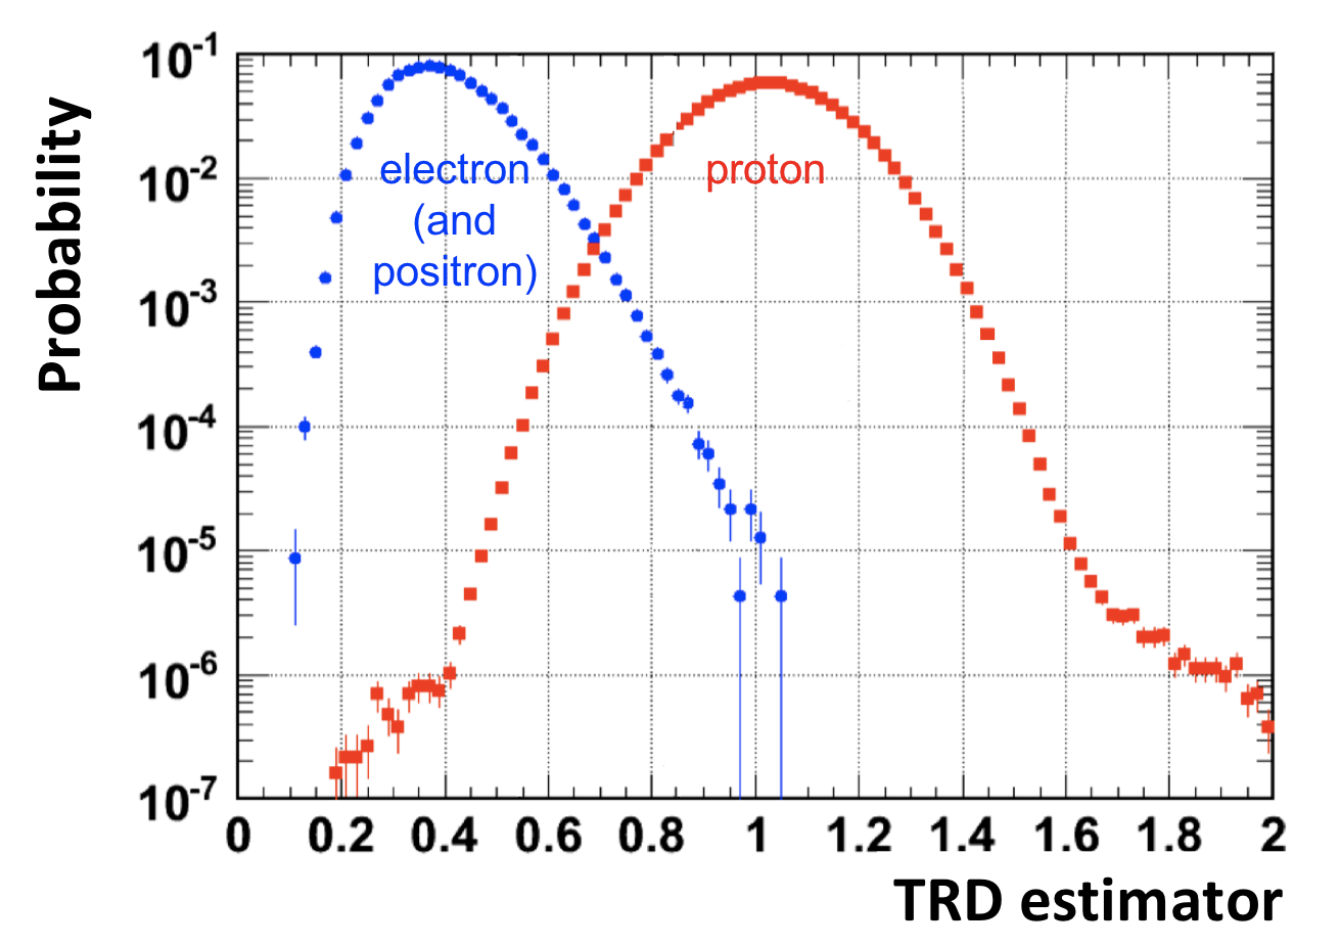
\includegraphics[width=0.80\textwidth]{Figures/chapter3/TRD/TRDEstimatorSeperation.png}
\includegraphics[width=1.00\textwidth]{Figures/chapter4/TRDLikelihood/{TRD_ChargeCorrectProtonTemplate_MC_B1042_pr.pl1.1800_7.6_all_Tree_positive_rigidity_14.1_15.3_pattern_0_bin_100_LogY_0.50}.pdf}
\caption[Seperation between the electrons and protons in $\Lambda_\mathrm{TRD}$ estimator.]{Seperation between the electrons and protons in $\Lambda_\mathrm{TRD}$ in the rigidity bin of 14.1 to 15.3 GV. The electrons and protons can be separated well in $\Lambda_\mathrm{TRD}$.}
\label{TRDEstimatorSeperation}
\end{figure}

the $\Lambda_\mathrm{TRD}$ provides separation power between electrons and protons. In figure \ref{TRDEstimatorSeperation}, the $\Lambda_\mathrm{TRD}$ is shown in the example rigidity bin of 14.1 to 15.3 GV, the electrons and protons can be distinguished well. At the 90\% electron efficiency range, the proton rejection power, which is defined as the inverse ratio of protons in this range, reaches more than $10^4$ \cite{TRDRejectionPowerPaper}. Similarly, the TRD likelihood estimator for the proton and the helium $\Lambda_{\mathrm{TRD}_{\mathrm{P/He}}}$ is defined as $-\rm{log}(\mathcal{L}_{p}/(\mathcal{L}_{p}+\mathcal{L}_{He}))$. \par


  

  
\section{Template Fit} \label{TempalteFitSection}

In this section, the template fits are shown in detail for the time-averaged analysis and the time-dependent analysis. The template fit is a method to extract signal and background events from the total event distribution. If the data distribution is $D(x)$ and it has $k$ components, then the goal of the template fit is to extract the event number of different components from the data distribution. In this analysis, the binned maximum likelihood fit is used. The fit is performed by minimizing the negative log-likelihood function $L$:

\begin{equation}
L = - \left ( \sum_{x}^{} D(x) \cdot {\rm{log}}(P(x)) - N_{{\rm{total}}} \right )
\end{equation}

where $N_{\rm{total}}$ is the total number of event, $P$ is the normalized likelihood, which is defined as the sum of the product of the number of events $N_{i}$ and the PDF of the template $P_i$:

\begin{equation}
P(x) = \sum_{i=1}^{k} N_{i} \cdot P_{i}(x)
\end{equation}

The minimization is achieved using the Minuit minimizer \cite{MinuitPaper}. The PDFs of templates are constructed before the template fit and the numbers of events are free parameters. By minimizing the negative log-likelihood function, the best-fit parameters, namely the number of events for signals and backgrounds, can be extracted.  \par

For different rigidity ranges, the template fit methods are different due to the sub-detector resolutions and background contributions. The selections used to obtain the signal and background templates will be discussed, and then the template fit result will be shown. In the time-dependent analysis, the template fit and the result in six Bartels Rotations will be given.   
 
%%%% Time averaged analysis
\subsection{Time-averaged analysis}
The first ingredient to construct the antiproton to proton flux ratio is the number of events. As the background levels can not be ignored, cut-based analysis is not enough to get clean signals. Therefore, in order to extract clean antiproton signals, the template fit method is used in this analysis. \par

In different rigidity ranges, the detector resolutions and background components are different, and the whole analysis is divided into three parts: low rigidity range (1.0 GV to 6.5 GV), intermediate rigidity range (3.0 to 19.5 GV), and high rigidity range (14.1 to 525 GV). The rigidity ranges are the same with the ones used in the previous AMS-02 antiproton analysis \cite{AMS02AntiprotonPRL2016}. In each range, a dedicated template fit method is used to get the antiproton signals, and the results in the overlappings from different template fit methods are used for crosschecks. \par

%% Low Range
\subsection*{Low Rigidity Range}
% 2D Template Fit method in TOF&TRD
In the low rigidity range, the dominant background sources are light particles. Except the electrons, the interaction between the incoming particles with the AMS-02 materials can produce secondary interaction particles like pions. These background components have to be separated from the antiproton signals. Since the particle's mass is calculated from rigidity and $\beta$ as given in equation \ref{MassEquation}, and the mass of the antiproton is much heavier than the background components in this range, the $\beta$ measurements of antiproton signal is different from the backgrounds in a specific rigidity bin. In this rigidity range, the TOF can be used to separate antiprotons and backgrounds by measuring the $\beta$. With the rigidity going up, the separation power from $\beta_{\rm{TOF}}$ decreases, and at the same time, the TRD separation power increases, so the $\Lambda_\mathrm{TRD}$ can take over afterwards in the intermediate rigidity range. A 2D template fit in $\Lambda_\mathrm{TRD}$ and $\beta_{\rm{TOF}}$ ($1/{\beta_{\rm{TOF}}}$) is used in the low rigidity range to have a smooth and stable separation power. The range in low rigidity is from 1.0 GV to 6.5 GV. The lower limit is due to the low statistics after the geometrical cutoff, and the higher limit is due to the $\beta_{\rm{TOF}}$ resolution. \par
% Templates
After the cuts and selections are applied, there are three major components in the data: antiprotons, electrons, and secondaries. The three templates must be constructed first to do the template fit. The antiproton template is taken from the ISS positive rigidity data since the clean proton data sample is easy to extract from it, and the rigidity sign does not impact the absolute value of the $\beta_{\rm{TOF}}$ and the $\Lambda_\mathrm{TRD}$. The electron and the secondaries templates are taken from the ISS negative rigidity data. To get the clean electron and secondaries samples from it, dedicated selections are applied for each sample respectively. Furthermore, after the preselection and selection introduced in Section \ref{DataSelectionSection}, the ISS data to be fitted should fulfill additional selection requirements in the low rigidity range. In table \ref{LowRigiditySelectionsForTemplates} the full list of selections is shown.  \par 

\begin{table}[h]
\setlength\tabcolsep{15pt}
\centering
\caption{List of selections to get all the templates and select further for the ISS data in the low rigidity range.} 
\label{LowRigiditySelectionsForTemplates}
\begin{tabular}{cc}
\hline \textbf{Antiproton Template}                                                                                                                             &  \textbf{Electron Template}                                                                                                                            \\
%\hline $\frac{1}{\beta_\mathrm{LowEdge}(R)} < \frac{1}{\beta_\mathrm{TOF}}-\frac{1}{\beta(R,m_{{\rm{p}}})}<0.2$    &  $\frac{1}{\beta_\mathrm{LowEdge}(R)}< \frac{1}{\beta_\mathrm{TOF}}-\frac{1}{\beta(R,m_{{\rm{p}}})}<0.2$  \\
%\hline $ \mathrm{\Lambda}_\mathrm{LowEdge}(R) < \Lambda_{\mathrm{TRD}} <  1.6 $                                                 &  $ \mathrm{\Lambda}_\mathrm{LowEdge}(R) < \Lambda_{\mathrm{TRD}} <  1.6 $                                                \\
\hline $ \Lambda_{\mathrm{TRD}_{\mathrm{P/He}}} < 0.1$                                                                                     &   Has $\beta$ measurement in RichAgl                                                                                                           \\
\hline TRD Number of tracks = 1                   &   | $ \beta_\mathrm{RICH} - \beta(R,m_{{\rm{e}}}) | <  0.002 $         \\
\hline TRD Number of hits < 40                     &   TRD Number of segments in XZ side = 1                                                     \\
\hline R > 0                                                    &   TRD Number of segments in YZ side = 1                                                     \\
\hline                                                              &   TRD Number of hits < 35                                                                             \\
\hline                                                              &    R < 0                                                                                                           \\
\hline       
\hline \textbf{Secondaries Template}                                                                   & \textbf{Further selections for ISS Data}               \\
%\hline $\frac{1}{\beta_\mathrm{LowEdge}(R)}< \frac{1}{\beta_\mathrm{TOF}}-\frac{1}{\beta(R,m_{{\rm{p}}})}<0.2$         & $\frac{1}{\beta_\mathrm{LowEdge}(R)}< \frac{1}{\beta_\mathrm{TOF}}-\frac{1}{ \beta(R,m_{{\rm{p}}}) }<0.2$  \\
%\hline $ \mathrm{\Lambda}_\mathrm{LowEdge}(R) < \Lambda_{\mathrm{TRD}} <  1.6 $                                                      & $ \mathrm{\Lambda}_\mathrm{LowEdge}(R) < \Lambda_{\mathrm{TRD}} <  1.6 $                                                \\
\hline Has $\beta$ measurement in RichAgl                                                                                                                 & $ \Lambda_{\mathrm{TRD}_{\mathrm{P/He}}} < 0.1$                                                                                     \\
\hline $ | \beta_\mathrm{RICH} - \beta(R,m_{{\rm{\pi}}}) | < 0.002 $   & TRD Number of segments in XZ = 1        \\
\hline TRD Number of segments in XZ side > 1                                                  & TRD Number of segments in YZ = 1       \\
\hline TRD Number of segments in YZ side > 1                                                  &  R < 0                                                       \\
\hline TRD Number of hits > 50                                                                           &                                                                  \\
\hline R < 0                                                                                                          &                                                                  \\  
\hline
\end{tabular}
\end{table}

%\begin{figure}[h]
%    \centering
%    \subfigure[]{
%        \includegraphics[width=0.51\textwidth, height=0.20\textheight ]{Figures/chapter4/TemplateFit/TimeAveragedPlot/Low/LowerEdge/{LowerEdge_TOF}.pdf} 
%    }\hspace{-0.9cm}
%    \subfigure[]{
%	\includegraphics[width=0.51\textwidth, height=0.20\textheight ]{Figures/chapter4/TemplateFit/TimeAveragedPlot/Low/LowerEdge/{LowerEdge_TRD}.pdf}
%    }
%    \caption[The rigidity dependence of a) 1/$\beta_{\rm{low}}$ and b) $\Lambda_{\mathrm{low}}$.]{The rigidity dependence of a) 1/$\beta_{\rm{LowEdge}}$ and b) $\Lambda_{\mathrm{LowEdge}}$ at the lower edge of the template fit range for 90\% signal efficiency. The red points correspond to the rigidity bin centers.}
%    \label{LowerEdgeOfLowTemplateFit}
%\end{figure}


In table \ref{LowRigiditySelectionsForTemplates}, $\beta_{\rm{RICH}}$ is the $\beta$ measurement from the RICH, $\beta(R,m)=\sqrt{\frac{R^2}{m^2+R^2}}$ is the $\beta$ value constructed with rigidity $R$ and mass $m$. Except for the cuts shown in the table, to remove most backgrounds before performing the template fit, additional template fit range cuts on $\beta_\mathrm{TOF}$ and $\Lambda_{\mathrm{TRD}}$ are applied to all the templates and ISS data to be fitted: $\frac{1}{\beta_\mathrm{LowEdge}(R)} < \frac{1}{\beta_\mathrm{TOF}}-\frac{1}{\beta(R,m_{{\rm{p}}})}<0.2$ and $ \mathrm{\Lambda}_\mathrm{LowEdge}(R) < \Lambda_{\mathrm{TRD}} <  1.6 $. $\beta_{\rm{LowEdge}}(R)$ and $\Lambda_{\mathrm{LowEdge}}(R)$ denote the low edge of the template fit range. By varying the low edges, the systematic uncertainty of the template fit can be evaluated. This will be discussed further later in Section \ref{SystematicUncertaintiesSection}. For the final time-averaged antiproton to proton flux ratio, the template fit result at 90\% signal efficiency is used. \par

%The rigidity dependence of $1/\beta_{\rm{LowEdge}}(R)$ and $\Lambda_{\mathrm{LowEdge}}(R)$ at the lower edge of the template fit range is shown in figure \ref{LowerEdgeOfLowTemplateFit}. \par

%Most cuts and selections are set using a fixed value except for the $1/\beta_{\rm{LowEdge}}(R)$ and $\Lambda_{\mathrm{LowEdge}}(R)$. These two cuts are the lower edge values of the template fit ranges and are rigidity-dependent. 
%$\beta(R,m_{{\rm{p}}})=\sqrt{\frac{R^2}{m_{{\rm{p}}}^2+R^2}}$ is the $\beta$ value constructed with rigidity and proton mass $m_{\rm{p}}$, 
%$\beta(R,m_{{\rm{e}}})=\sqrt{\frac{R^2}{m_{{\rm{e}}}^2+R^2}}$ is the $\beta$ value constructed with rigidity and electron mass $m_{\rm{e}}$, 
%$\beta(R,m_{{\rm{\pi}}})=\sqrt{\frac{R^2}{m_{{\rm{\pi}}}^2+R^2}}$ is the $\beta$ value constructed with rigidity and pion mass $m_{\rm{\pi}}$. \par


%%%%%%%%%%%%%%%%%%%%%%%%%%%%%%%%%%%%%%%%%%%%%%%%%%%
% Template Fit (Old)
%Once the templates are obtained, the template fit can be performed. In this analysis, the binned maximum likelihood fit is used. For example, in the low rigidity range, the likelihood function is written as:
%\begin{equation}
%f(\mathcal{L})=N_{\bar{p}} \cdot T_{\bar{p}}(\mathcal{L}) + N_{e^{-}} \cdot T_{e^{-}}(\mathcal{L}) + N_{s} \cdot T_{s}(\mathcal{L})
%\end{equation}
%where the $T_{\bar{p}}(\mathcal{L})$, $T_{e^{-}}(\mathcal{L})$ and $T_{s}(\mathcal{L})$ are the normalized antiproton, electron and secondaries templates respectively, and the $N_{\bar{p}}$, $N_{e^{-}}$ and $N_{s}$ are the free parameters in the fit, which are correspondent to the event numbers of these components. \par
%%%%%%%%%%%%%%%%%%%%%%%%%%%%%%%%%%%%%%%%%%%%%%%%%%%

\begin{figure}[htbp]
    \centering
    \subfigure[]{
         \includegraphics[width=1.0\textwidth,  trim=0.7cm 4.6cm 10cm 0.45cm, clip]{Figures/chapter4/TemplateFit/TimeAveragedPlot/Low/TemplateFit/fullrange/2DShowData/{FitResult_tof_2.97_3.29_pass7.8_TRDeff_1.00_TOFeff_1.00}.pdf} %xleftupper, yleftbottom, xrightbottom, yrightupper
         \label{LowRangeDataPlot}
    }
    \subfigure[]{
         \includegraphics[width=1.0\textwidth, trim=10.7cm 4.6cm 0 0.45cm, clip]{Figures/chapter4/TemplateFit/TimeAveragedPlot/Low/TemplateFit/fullrange/2DShowData/{FitResult_tof_2.97_3.29_pass7.8_TRDeff_1.00_TOFeff_1.00}.pdf}
         \label{LowRangeFitPlot}
    }
    \caption[Negative ISS data and Fit result in 2.97 to 3.29 GV]{a) Negative rigidity ISS data in the rigidity range of 2.97 to 3.29 GV in 1/$\beta_\mathrm{TOF}$ and $\Lambda_\mathrm{TRD}$ space. In the Y axis, 1/$\beta$ calculated with rigidity and antiproton mass is subtracted from the value of 1/$\beta_\mathrm{TOF}$, so the distribution of antiproton can be normalized to be around 0. Antiproton signal, electron and secondaries background components are seen in this plot. To remove the most backgrounds, $\Lambda_\mathrm{TRD}$ cut of 0.7 is applied in this plot. b) The 2D template fit result in the same rigidity bin of 2.97 to 3.29 GV in 1/$\beta_\mathrm{TOF}$ and $\Lambda_\mathrm{TRD}$ space.} 
\end{figure}


\begin{figure}[htbp]
    \centering
    \subfigure[]{
         \includegraphics[width=0.9\textwidth, height=0.43\textheight]{Figures/chapter4/TemplateFit/TimeAveragedPlot/Low/TemplateFit/fullrange/TOF-0.3TRD0.7/TOF-0.1TRD0.9/{1_TofBeta_Y_tof_LogY_2.97_3.29_pass7.8_TRDeff_1.00_TOFeff_1.00}.pdf}
    }
    \vspace{-0.2cm}
    \par 
    \subfigure[]{
	\includegraphics[width=0.9\textwidth, height=0.43\textheight]{Figures/chapter4/TemplateFit/TimeAveragedPlot/Low/TemplateFit/fullrange/TOF-0.3TRD0.7/TOF-0.1TRD0.9/{TrdLikelihood_X_tof_LogY_2.97_3.29_pass7.8_TRDeff_1.00_TOFeff_1.00}.pdf}	
    }
    \caption[Example template fit in the low rigidity range of 2.97 to 3.29 GV.]{Example template fit in the low rigidity range of 2.97 to 3.29 GV. a) 1/$\beta_\mathrm{TOF}$ projection. In this projection, 1/$\beta$ calculated with rigidity and antiproton mass is subtracted from the value of 1/$\beta_\mathrm{TOF}$. b) $\Lambda_\mathrm{TRD}$ projection.}
    \label{LowRigidityExampleTemplateFitProjections}
\end{figure}

In figure \ref{LowRangeDataPlot}, the negative rigidity ISS data in the rigidity range of 2.97 to 3.29 GV is shown in 1/$\beta_\mathrm{TOF}$ and $\Lambda_\mathrm{TRD}$ space. The three components are antiprotons, electrons and interaction secondaries. $\Lambda_\mathrm{TRD}$ cut of 0.7 is applied in this plot to remove the most backgrounds of electrons and interaction secondaries. In figure \ref{LowRangeFitPlot}, an example template fit in this rigidity range is shown. To illustrate the separation, the 2D template fit is shown in two projections in figure \ref{LowRigidityExampleTemplateFitProjections}. In 1/$\beta_\mathrm{TOF}$ projection, further cut of $\Lambda_{\rm{TRD}}>0.9$ is applied to reduce the backgrounds; similarly in $\Lambda_\mathrm{TRD}$ projection, further cut of 1/$\beta_\mathrm{TOF}$-1/$\beta(R,m_{p})$>-0.1 is applied. Since it is a 2D template fit, the $\chi^2$/ndf is calculated individually in the two projections. \par

The template fits give the number of antiproton events in the low rigidity range. The proton number is obtained after selections introduced in Section \ref{DataSelectionSection} and further selections for ISS data in table \ref{LowRigiditySelectionsForTemplates} but $R>0$. In figure \ref{PbarNumbersInLowRigidityRange} the number of antiproton and proton events as a function of the rigidity obtained is given. 
%The corresponding $\chi^2$/ndf values of the template fits are given in figure \ref{Chi2OfFitInLowRigidityRange}.  \par

\begin{figure}[H]
\includegraphics[width=1.00\textwidth]{Figures/chapter4/TemplateFit/TimeAveragedPlot/Low/{NumberPbarAndProtonPlot_LowRange_pass78}.pdf}
\caption[The number of antiproton and proton events obtained in the low rigidity range.]{The numbers of antiproton and proton events as function of the rigidity obtained in the low rigidity range.}
\label{PbarNumbersInLowRigidityRange}
\end{figure}

%\begin{figure}[H]
%\includegraphics[width=1.00\textwidth]{Figures/chapter4/TemplateFit/TimeAveragedPlot/Low/FitResult/{chi2_tof_pass7.8_TRDEff_0.94_TOFEff_0.95}.pdf}
%\caption{The $\chi^2$/ndf of the template fits in the low rigidity range.}
%\label{Chi2OfFitInLowRigidityRange}
%\end{figure}


%% Intermediate Range
\subsection*{Intermediate Rigidity Range}
% Template Fit method in TRD
In the intermediate rigidity range, the 2D template fit in $\beta_{\rm{TOF}}$ and $\Lambda_\mathrm{TRD}$ is replaced by a 1D template fit in $\Lambda_\mathrm{TRD}$ since the separation power of $\beta_{\rm{TOF}}$ decreases with the rigidity going up and provides little power in this rigidity range. Above 20 GV, the component of charge confused protons gradually increases, so it has to be added as an additional template. Therefore the 1D template fit can only be implemented up to around 20 GV. \par

% Templates
In the intermediate rigidity range, the interaction secondaries component is negligible. Therefore, the templates in this rigidity range are only formed for antiprotons and electrons. Like the template fit in the low rigidity range, the templates are also taken from the ISS data. The antiproton template is taken from positive rigidity data, and the electron template is taken from negative rigidity data. The dedicated selections for ISS data in the intermediate rigidity range are applied before the template fit. In table \ref{IntermediateRigiditySelectionsForTemplates}, the full list of selections that are used for the ISS data and in order to form the templates is given.  \par

\begin{table}[htbp]
\setlength\tabcolsep{15pt}
\centering
\caption{List of selections to get all the templates and select further for the ISS data in the intermediate rigidity range.} 
\label{IntermediateRigiditySelectionsForTemplates}
\begin{tabular}{cc}
\hline \textbf{Antiproton Template}      &  \textbf{Electron Template}           \\
%\hline PatternCut                             &  PatternCut                                    \\
%\hline $ \mathrm{\Lambda}_\mathrm{LowEdge}(R) < \Lambda_{\mathrm{TRD}} < 2 $  &  $ \mathrm{\Lambda}_\mathrm{LowEdge}(R) < \Lambda_{\mathrm{TRD}} < 2 $  \\
\hline $\beta_\mathrm{RICH}<\beta_\mathrm{high}(R)$                                             &   TRD Number of hits < 35                          \\
\hline TRD Number of segments in XZ side = 1                                                                  &   ECALBDT > 0.5                                         \\
\hline TRD Number of segments in YZ side = 1                                                                  &   TRD Number of segments in XZ side = 1         \\
\hline R > 0                                                                                                                   &   TRD Number of segments in YZ side = 1        \\
\hline                                                                                                                            & R < 0                                                           \\
%\hline                                                                                                                         &  $TRDLogLikelihood>-1.5$                         \\
\hline \textbf{Further selections for ISS Data}                                                                            &        \\
%\hline PatternCut                                                                                                      &        \\
%\hline  $ \mathrm{\Lambda}_\mathrm{LowEdge}(R) < \Lambda_{\mathrm{TRD}} < 2 $ &        \\
\hline  $\beta_\mathrm{RICH}<\beta_\mathrm{high}(R)$                                            &        \\
\hline  TRD Number of segments in XZ side = 1                                                                 &        \\
\hline  TRD Number of segments in YZ side = 1                                                                  &        \\
\hline  R < 0                                                                                                                   &        \\
\hline
\end{tabular}
\end{table}

\begin{figure}[htbp]
\centering
%\includegraphics[width=1.00\textwidth]{Figures/chapter4/TemplateFit/TimeAveragedPlot/intermediate/TemplateFit/{FitResult_0124_free_pass7.8_10.1_11_TRDEff_0.90}.pdf}
\includegraphics[width=1.00\textwidth]{Figures/chapter4/TemplateFit/TimeAveragedPlot/intermediate/TemplateFit_FullRange/{FitResult_LogY_0124_free_pass7.8_5.9_6.47_TRDEff_1.00}.pdf}
%\caption{Example template fit in the intermediate rigidity range of 10.1 to 11.0 GV.}
\caption[Example template fit in the intermediate rigidity range of 5.9 to 6.47 GV.]{Example template fit in the intermediate rigidity range of 5.9 to 6.47 GV. To reduce the most electrons, the template fit is performed on the right side of the dashed line, which corresponds to around 99\% antiproton signal efficiency.}
\label{ExampleTemplateFitInIntermediateRange}
\end{figure}

In table \ref{IntermediateRigiditySelectionsForTemplates}, the ECALBDT estimator is a value trained with ECAL response variables and can provide separation power between protons and electrons. If the particles go through the ECAL, a clean electron sample can be obtained by applying a cut of 0.5 on ECALBDT. To avoid the light particles background, if there is a $\beta_{\rm{RICH}}$ measurement then the value has to be less than $\beta_\mathrm{high}(R)$ to restrict the signal range. The $\beta_\mathrm{high}(R)$ is determined by 90\% antiproton signal efficiency. Except for the cuts in this table, to remove most backgrounds before performing the template fit, an additional template fit range cut on $\Lambda_{\mathrm{TRD}}$ is applied to all the templates and ISS data to be fitted like described in the low rigidity range.  \par 


% Example Fit
In figure \ref{ExampleTemplateFitInIntermediateRange}, an example template fit in the rigidity range of 5.9 to 6.47 GV is shown. The antiproton signal can be separated well from the electron background. To reduce the most background of electrons, the template fit range is set to around 99\% antiproton signal efficiency (the dashed line).

The template fits give the number of antiproton events in the intermediate rigidity range. The proton number is obtained after selections introduced in Section \ref{DataSelectionSection} and further selections for ISS data in table \ref{IntermediateRigiditySelectionsForTemplates} but $R>0$. The obtained antiproton and proton numbers are shown in figure \ref{PbarNumbersInIntermediateRigidityRange}. 
%The corresponding $\chi^2$/ndf values of the template fits in the intermediate rigidity range are given in Figure \ref{Chi2OfFitInIntermediateRigidityRange}. \par

\begin{figure}[H]
\includegraphics[width=1.00\textwidth]{Figures/chapter4/TemplateFit/TimeAveragedPlot/intermediate/{NumberPbarAndProtonPlot_IntermediateRange_pass78}.pdf}
\caption[The number of antiproton and proton events obtained in the intermediate rigidity range.]{The numbers of antiproton and proton events as function of the rigidity obtained in the intermediate rigidity range.}
\label{PbarNumbersInIntermediateRigidityRange}
\end{figure}

%\begin{figure}[t]
%\includegraphics[width=1.00\textwidth]{Figures/chapter4/TemplateFit/TimeAveragedPlot/intermediate/TemplateFit/{chi2dof_0124_free_pass7.8binmerge1_TRDEff_0.90}.pdf}
%\caption{The $\chi^2$/ndf of the template fits in the intermediate rigidity range.}
%\label{Chi2OfFitInIntermediateRigidityRange}
%\end{figure}

%% High Range
\subsection*{High Rigidity Range}

% Template Fit method in CC vs. TRD
In the high rigidity range, the contribution of charge confused protons increases. Therefore, the $\Lambda_{\rm{CC}}$ trained in Section \ref{chargeconfusion} is used to separate antiprotons and charge confused protons. For electron separation, the TRD provides separation power, like in the low and intermediate rigidity ranges. In summary, a 2D template fit in $\Lambda_{\rm{CC}}$ and $\Lambda_\mathrm{TRD}$ is performed in this range to get the antiproton signal. \par

\begin{figure}[tph]
    \centering
    
    \subfigure[]{
         \includegraphics[width=0.90\textwidth,  trim=0.5cm 7.5cm 10cm 0.7cm, clip]{Figures/chapter4/TemplateFit/TimeAveragedPlot/high/TemplateFit/{FitResult_Pattern_0_VGG16NN_175_211_cccut_0.20_CCN_20_TRDN_20}.pdf} %xleftupper, yleftbottom, xrightbottom, yrightupper
         \label{HighRangeDataPlot} 
    }
    \vspace{-0.2cm}
    \par
    \subfigure[]{
         \includegraphics[width=0.9\textwidth, trim=10.5cm 7.5cm 0 0.7cm, clip]{Figures/chapter4/TemplateFit/TimeAveragedPlot/high/TemplateFit/{FitResult_Pattern_0_VGG16NN_175_211_cccut_0.20_CCN_20_TRDN_20}.pdf}
         \label{HighRangeFitPlot}
    }
    \caption[Negative rigidity ISS data and fit result in the rigidity range of 175 to 211 GV in $\Lambda_{\rm{CC}}$ and $\Lambda_\mathrm{TRD}$ space.]{a) Negative rigidity ISS data in the rigidity range of 175 to 211 GV in $\Lambda_{\rm{CC}}$ and $\Lambda_\mathrm{TRD}$ space. Three components of antiprotons, electrons and charge confused protons are seen in this plot. To remove most backgrounds of charge confused protons, $\Lambda_{\rm{CC}}$ cut of 0.2 is applied. b) The 2D template fit result in the same rigidity bin of 175 to 211 GV in $\Lambda_{\rm{CC}}$ and $\Lambda_\mathrm{TRD}$ space.}    
\end{figure}


\begin{figure}[htbp]
    \centering
    \subfigure[]{
        \includegraphics[width=0.9\textwidth, height=0.43\textheight]{Figures/chapter4/TemplateFit/TimeAveragedPlot/high/TemplateFit/{CCprojection_Pattern_0_VGG16NN_175_211_cccut_0.20_CCN_20_TRDN_20}.pdf} 
    }
     \vspace{-0.2cm}
    \par
    \subfigure[]{
	\includegraphics[width=0.9\textwidth, height=0.43\textheight]{Figures/chapter4/TemplateFit/TimeAveragedPlot/high/TemplateFit/{TRDprojection_Pattern_0_VGG16NN_175_211_cccut_0.20_CCN_20_TRDN_20}.pdf} 
    }
    \caption[Example template fit in the high rigidity range of 175 to 211 GV.]{Example template fit in the high rigidity range of 175 to 211 GV. a) In the $\Lambda_{\rm{CC}}$ projection, $\Lambda_{\rm{TRD}}$>0.7 is applied and antiproton and charge confused proton can be separated well in this projection.  b) In the $\Lambda_\mathrm{TRD}$ projection, $\Lambda_{\rm{CC}}$>0.75 is applied and antiproton and electron can be separated well.}
    \label{ExampleTemplateFitInHighRigidityRange}
\end{figure}

% Tracker Pattern usage in Rigidity ranges 
As shown in figure \ref{TrackerResolutions}, different tracker patterns have different rigidity resolutions. To maximize the statistics and maintain the accuracy of rigidity measurement, the requirement of tracker patterns changes as rigidity goes up: No hit in tracker layers 1 and 9 is required below 38.9 GV; hit in either layer 1 and 9 is required from 38.9 to 147 GV; hit in layer 9 is required from 147 to 175 GV. Above 175 GV, hits in layers 1 and 9 are required. This selection requirement is the same as the one used in the previous AMS-02 publication \cite{AMS02AntiprotonPRL2016}. From 80.5 GV, every two rigidity bins are merged to increase the statistics. \par

% Templates
In the 2D template fit, the three templates are antiprotons, electrons, and charge confused protons. The antiproton template is taken from the ISS positive rigidity data, and the electron template is taken from the ISS negative rigidity data by ECALBDT. Finally, the charge confused proton template is formed by using proton MC simulation samples by selecting events with negative rigidity. To avoid the contamination of helium, the $\Lambda_{\mathrm{TRD}_{\mathrm{P/He}}} < 0.3$ cut is applied for the negative rigidity data before the template fit. \par      %%--trd low 0.0 --trd high 1.6
%the electron template is taken from the ISS negative rigidity data by ECALBDT to be larger than zero

% Table of selection (Commented Out)
\begin{comment}
\begin{table}[h]
\setlength\tabcolsep{15pt}
\centering
\caption{List of selections for templates}
\label{HighRigiditySelectionsForTemplates}
\begin{tabular}{cc}
\hline \textbf{Antiproton template}                         &  \textbf{Electron Template}                         \\
\hline         $-1<ECALBDT<0$                                 &  $0<ECALBDT$                                       \\
\hline         $\rm{TRDLikelihood_{P/He}} < 0.3$      &   $\rm{TRDLikelihood_{P/He}} < 0.3$      \\
\hline \textbf{Charge confused proton Template}  &  \textbf{Negative Rigidity Data}                  \\
\hline         $-1<ECALBDT<0$                                 &   $-2<ECALBDT<0$                                 \\
\hline         $\rm{TRDLikelihood_{P/He}} < 0.3$,     &   $\rm{TRDLikelihood_{P/He}} < 0.3$      \\
\hline
\end{tabular}
\end{table}
\end{comment}

% Example Fit
To cut away the most background of charge confused protons, the template fit is performed in $\Lambda_{\rm{CC}}>0.2$ range. In figure \ref{HighRangeDataPlot}, the negative rigidity ISS data in the rigidity range of 175 to 211 GV is shown in $\Lambda_{\rm{CC}}$ and $\Lambda_\mathrm{TRD}$ space. The three components of antiprotons, electrons and charge confused protons are indicated in this figure. In figure \ref{HighRangeFitPlot}, an example template fit in this rigidity range is shown. To illustrate the separation, the 2D template fit is shown in two projections in figure \ref{ExampleTemplateFitInHighRigidityRange}. In $\Lambda_{\rm{CC}}$ projection, $\Lambda_{\rm{TRD}}$>0.7 is applied to show the separation between antiprotons and charge confused protons. In $\Lambda_\mathrm{TRD}$ projection, $\Lambda_{\rm{CC}}$>0.75 is applied to show the separation between antiprotons and electrons. Since it is a 2D template fit, the $\chi^2$/ndf is calculated individually in the two projections. \par
%In $\Lambda_{\rm{CC}}$ projection, further cut of $\Lambda_{\rm{TRD}}>0.5$ is applied to show the separation between antiprotons and charge confused protons. In $\Lambda_\mathrm{TRD}$ projection, further cut of  $\Lambda_{\rm{CC}}>0.4$ is applied to show the separation between antiprotons and electrons. \par

%The number of antiprotons obtained from the 2D template fit and the number of protons after the selections introduced in Section \ref{DataSelectionSection} are given in figure \ref{PbarNumbersInHighRigidityRange}.  
The numbers of antiprotons and protons obtained in the high rigidity range are given in figure \ref{PbarNumbersInHighRigidityRange}.  


%For example, the corresponding $\chi^2$/ndf in the full span is given in \ref{Chi2OfFitInHighRigidityRange}. \par 

\begin{figure}[hptb]
\includegraphics[width=1.00\textwidth]{Figures/chapter4/TemplateFit/TimeAveragedPlot/high/{NumberPlot_AllPatternsOverRigidityBinWidthpass78}.pdf}
\caption[The antiproton and proton numbers obtained in the high rigidity range.]{The antiproton and proton numbers obtained in the high rigidity range. The dashed vertical lines are the boundary of the usage of different tracker patterns. To avoid the jump due to the merge of rigidity bins from 80.5 GV, the antiproton and proton numbers are divided by the rigidity bin width to have a smooth curve.}
\label{PbarNumbersInHighRigidityRange}
\end{figure}

Once the template fits in the three rigidity ranges are performed, the antiproton numbers from 1.0 to 525 GV can be obtained. In total, 481959 antiprotons are selected from the template fits. \par

%\begin{figure}[H]
%\includegraphics[width=1.00\textwidth]{Figures/chapter4/TemplateFit/TimeAveragedPlot/high/FitResult/{Chi2dof_Pattern_0_pass7.8_VGG16NN}.pdf}
%\caption{The $\chi^2$/ndf of template fit in full span in the high rigidity range.}
%\label{Chi2OfFitInHighRigidityRange}
%\end{figure}



%In figure \ref{PbarTimeAveragedNumbers}, the antiproton number plot is shown. 
%\begin{figure}[H]
%\centering
%\includegraphics[width=1.00\textwidth]{Figures/chapter4/TemplateFit/TimeAveragedPlot/{NumberPlot_pass78_AllRange}.pdf}
%\caption{The antiproton numbers get from the template fit result.}
%\label{PbarTimeAveragedNumbers}
%\end{figure}


%%%% Time-dependent analysis
\subsection{Time-dependent analysis}

% Template Fit method
For the time-dependent analysis, the template fit strategy is the same as the one used in the time-averaged analysis. The data is divided into time bins with a width equal to the duration of six Bartels Rotations each. In each time bin, a template fit is performed to get the antiproton to proton ratio. Due to the limited statistics in each time bin, the rigidity binning is altered in the following way: every two original neighboring rigidity bins are now merged to form a new bin. In this way, an increase in statistics in each new bin is accomplished. \par

% Time Dependent Template
The template selections are the same as the ones used in the time-averaged analysis. The only difference is the template fit range. To increase the statistics, the signal efficiency is increased from 90\% to 95\% in the low rigidity range and from 90\% to 98\% in the intermediate rigidity range. \par

Since the templates are taken from the ISS data, the shapes of the templates are time-dependent. To visualize the time dependence, all the templates are parameterized in the distribution core range in the following way: In the $\Lambda_\mathrm{TRD}$ dimension, the antiproton, electron and secondaries are parameterized by a Novosibirsk function $N(x;\mu,\sigma,\tau)$, and in the 1/$\beta_\mathrm{TOF}$ dimension, the antiproton, electron and secondaries are parameterized by a Gaussian function $G(x; \mu,\sigma)$: \par

\begin{figure}[hptb]
\centering
\includegraphics[width=1.00\textwidth]{Figures/chapter4/TemplateFit/TimeDependentPlot/TimeDependentTemplate/TRD/{TemplateFit_TRD_6.47_7.76_78}.pdf}
\caption[The parameterizations of the normalized antiproton and electron templates.]{The parameterizations of the normalized antiproton and electron templates by Novosibirsk functions in the rigidity range of 6.47 to 7.76 GV with data collected from Feb.18.2017 to Jul.30.2017.}
\label{PparameterizationsTemplate}
\end{figure}

\begin{equation}
\begin{aligned}
G(x; \mu,\sigma) &= \frac{1}{\sqrt{2 \pi \sigma^2}}{\rm{exp}} \left(-\frac{(x-\mu)^2}{2\sigma^2} \right), \\
N(x;\mu,\sigma,\tau)&={\rm{exp}}\left( -\frac{1}{2} \left( \frac{({\rm{ln}}(\lambda(x; \mu,\sigma,\tau)))^2}{\tau^2}+\tau^2  \right)  \right), {\rm{where}}\\
\lambda(x; \mu,\sigma,\tau)&=1+\tau(x-\mu)\frac{{\rm{sinh}}(\tau\sqrt{{\rm{ln}}4})}{\sigma\tau\sqrt{{\rm{ln}}4}}
\end{aligned}
\end{equation}

% TRD side:
For an illustration of parameterization in the $\Lambda_\mathrm{TRD}$ dimension, the parameterizations of the normalized antiproton and electron templates in the rigidity range of 6.47 to 7.76 GV with data collected from Feb.18.2017 to Jul.30.2017 is shown as an example in figure \ref{PparameterizationsTemplate}. 

\begin{figure}[hptb]
    \centering
    \subfigure[]{
        \includegraphics[width=0.49\textwidth, height=0.23\textheight]{Figures/chapter4/TemplateFit/TimeDependentPlot/TimeDependentTemplate/TRD/Antiproton/{Antiproton_TRD_6.47_7.76_miu}.pdf} 
    }
    \hspace{-0.7cm}
    \subfigure[]{
	\includegraphics[width=0.49\textwidth, height=0.23\textheight]{Figures/chapter4/TemplateFit/TimeDependentPlot/TimeDependentTemplate/TRD/Antiproton/{Antiproton_TRD6.47_7.76_sigma}.pdf} 
    } 
    \subfigure[]{
        \includegraphics[width=0.49\textwidth, height=0.23\textheight]{Figures/chapter4/TemplateFit/TimeDependentPlot/TimeDependentTemplate/TRD/Electron/{Electron_TRD_6.47_7.76_miu}.pdf} 
    } 
    \hspace{-0.7cm}
    \subfigure[]{
	\includegraphics[width=0.49\textwidth, height=0.23\textheight]{Figures/chapter4/TemplateFit/TimeDependentPlot/TimeDependentTemplate/TRD/Electron/{Electron_TRD6.47_7.76_sigma}.pdf} 
    }
    %\vspace{-10mm}        
    \caption[Time-dependence of the a) $\mu_{\rm{\bar{p},TRD}}$ b) $\sigma_{\rm{\bar{p},TRD}}$ c) $\mu_{\rm{e^{-},TRD}}$ d) $\sigma_{\rm{e^{-},TRD}}$ in 6.47 to 7.76 GV.]{Time-dependence of the a) $\mu_{\rm{\bar{p},TRD}}$ b) $\sigma_{\rm{\bar{p},TRD}}$ c) $\mu_{\rm{e^{-},TRD}}$ d) $\sigma_{\rm{e^{-},TRD}}$ in the rigidity range of 6.47 to 7.76 GV. The parameters of the electron template show significant structures up to the end of 2012, where the TRD gas parameters were being optimized. After that, both parameters of antiproton and electron templates are changing due to the decrease of the Xe partial pressure in the TRD.}
    \label{TimeDependenceParameters}
\end{figure}

\begin{figure}[htbp]
    \centering
    \subfigure[]{
        \includegraphics[width=0.49\textwidth, height=0.23\textheight]{Figures/chapter4/TemplateFit/TimeDependentPlot/TimeDependentTemplate/TOF/Antiproton/{Antiproton_TOF_3.64_4.43_miu}.pdf} 
    }
    \hspace{-0.7cm}
    \subfigure[]{
	\includegraphics[width=0.49\textwidth, height=0.23\textheight]{Figures/chapter4/TemplateFit/TimeDependentPlot/TimeDependentTemplate/TOF/Antiproton/{Antiproton_TOF3.64_4.43_sigma}.pdf} 
    } 
    \subfigure[]{
        \includegraphics[width=0.49\textwidth, height=0.23\textheight]{Figures/chapter4/TemplateFit/TimeDependentPlot/TimeDependentTemplate/TOF/Electron/{Electron_TOF_3.64_4.43_miu}.pdf} 
    } 
    \hspace{-0.7cm}
    \subfigure[]{
	\includegraphics[width=0.49\textwidth, height=0.23\textheight]{Figures/chapter4/TemplateFit/TimeDependentPlot/TimeDependentTemplate/TOF/Electron/{Electron_TOF3.64_4.43_sigma}.pdf} 
    }  
    \subfigure[]{
        \includegraphics[width=0.49\textwidth, height=0.23\textheight]{Figures/chapter4/TemplateFit/TimeDependentPlot/TimeDependentTemplate/TOF/Pion/{Pion_TOF_3.64_4.43_miu}.pdf} 
    } 
    \hspace{-0.7cm}
    \subfigure[]{
	\includegraphics[width=0.49\textwidth, height=0.23\textheight]{Figures/chapter4/TemplateFit/TimeDependentPlot/TimeDependentTemplate/TOF/Pion/{Pion_TOF3.64_4.43_sigma}.pdf}  
    }
    \caption[Time-dependence of the a) $\mu_{\rm{\bar{p}},TOF}$ b) $\sigma_{\rm{\bar{p}},TOF}$ c) $\mu_{\rm{e^{-}},TOF}$ d) $\sigma_{\rm{e^{-}},TOF}$ e) $\mu_{\rm{secondaries},TOF}$ f) $\sigma_{\rm{secondaries},TOF}$ in 3.64 to 4.43 GV.]{Time-dependence of the a) $\mu_{\rm{\bar{p}},TOF}$ b) $\sigma_{\rm{\bar{p}},TOF}$ c) $\mu_{\rm{e^{-}},TOF}$ d) $\sigma_{\rm{e^{-}},TOF}$ e) $\mu_{\rm{secondaries},TOF}$ f) $\sigma_{\rm{secondaries},TOF}$ in the rigidity range of 3.64 to 4.43 GV. No obvious trend is observed in the mean values but the distributions of sigma show rising trends in all three components, this could be due to the aging of the scintillators.}
    \label{TimeDependenceTOFPara}
\end{figure}


For the antiproton template, the time dependence can be described by the mean value $\mu_{\rm{\bar{p},TRD}}$ and width $\sigma_{\rm{\bar{p}},TRD}$. For the electron template, the time dependence can be described by the mean value $\mu_{\rm{e^{-}},TRD}$ and width $\sigma_{\rm{e^{-}},TRD}$. The time dependence of the four parameters in the rigidity range of 6.47 to 7.76 GV is shown in figure \ref{TimeDependenceParameters}.


% TOF side:
%For an illustration of parameterization in the 1/$\beta_\mathrm{TOF}$ dimension, the parameterizations of the normalized antiproton, electron and secondaries templates in the rigidity range of X.XX to X.XX GV with data collected from Feb.18.2017 to Jul.30.2017 is shown as an example in figure \ref{XXX}.

For the 1/$\beta_\mathrm{TOF}$ dimension, the cores of the normalized antiproton, electron and secondaries templates are parametrized by Gaussian functions. The time dependence of the antiproton template can be described by the mean value $\mu_{\rm{\bar{p}},TOF}$ and width $\sigma_{\rm{\bar{p}},TOF}$, the time dependence of the electron template can be described by the mean value $\mu_{\rm{e^{-}},TOF}$ and width $\sigma_{\rm{e^{-}},TOF}$, the time dependence of the secondaries can be described by the mean value $\mu_{\rm{secondaries},TOF}$ and width $\sigma_{\rm{secondaries},TOF}$. The six parameters in an example rigidity range of 3.64 to 4.43 GV are shown in figure \ref{TimeDependenceTOFPara}.\par



% Example Template Fit
An example template fit in the rigidity range of 6.47 to 7.76 GV is given in figure \ref{TimeDependentTemplateFitInInermediate}. The fitted data is six Bartels Rotations data taken from Feb.18.2017 to Jul.30.2017. \par

\begin{figure}[htpb]
\centering
%\includegraphics[width=1.00\textwidth]{Figures/chapter4/TemplateFit/TimeDependentPlot/intermediate/FitPlot/{FitResult_0124_free_6.47_7.76_index_114_LogY}.pdf}
%\caption{Example template fit in the rigidity range of 6.47 to 7.76 GV with data collected from Jan.07.2020 to June.17.2020.}  % 1578355200 to 1592352000
\includegraphics[width=1.00\textwidth]{Figures/chapter4/TemplateFit/TimeDependentPlot/intermediate/FitPlot_FullRange/{FitResult_0124_free_6.47_7.76_index_78_TRDEff_1.00_LogY}.pdf}
\caption[Example template fit in 6.47 to 7.76 GV with data from Feb.2017 to Jul.2017.]{Example template fit in the rigidity range of 6.47 to 7.76 GV with data collected from Feb.18.2017 to Jul.30.2017.}  % 1494374400 to 1508371200
%To collect the most statistics of antiproton signal, no cut on the $\Lambda_\mathrm{TRD}$ is applied.
\label{TimeDependentTemplateFitInInermediate}
\end{figure}

The obtained antiproton numbers in 6.47 to 7.76 GV for the 23 groups containing data of six Bartels Rotations each is shown in figure \ref{PbarNumbersInTimeDependentIntermediateRange}. The corresponding values of the $\chi^2$/ndf are given in figure \ref{Chi2dofOfTimeDependentIntermediateRange}.  

\begin{figure}[htpb]
\centering
\includegraphics[width=1.00\textwidth, height=0.4\textheight]{Figures/chapter4/TemplateFit/TimeDependentPlot/intermediate/FitResult/{AntiprotonNumber_6BartalRotation_0124_free_binmerge2_6.47_7.76}.pdf}
\caption[Antiproton numbers in 6.47 to 7.76 GV with six Bartels' Rotation.]{The antiproton numbers obtained from the template fit results in the rigidity range of 6.47 to 7.76 GV with six Bartels' Rotation time resolution. To avoid jumps due to the measuring time (see Section \ref{MeasuringTimeSection}), the numbers are divided by the measuring time in each six Bartels' Rotation time bin.}
\label{PbarNumbersInTimeDependentIntermediateRange}
\end{figure}

\begin{figure}[htpb]
\centering
\includegraphics[width=1.00\textwidth, height=0.4\textheight]{Figures/chapter4/TemplateFit/TimeDependentPlot/intermediate/FitResult/{Chi2dof_6BartalRotation_0124_free_binmerge2_6.47_7.76}.pdf}
\caption[$\chi^2$/ndf of the fits in 6.47 to 7.76 GV with six Bartel's Rotation.]{$\chi^2$/ndf of the template fits in the rigidity range of 6.47 to 7.76 GV with six Bartel's Rotation time resolution.}
\label{Chi2dofOfTimeDependentIntermediateRange}
\end{figure}




%\subsection*{Low Rigidity Range}
% Template Fit method 
%In the low rigidity range, the 2D template fit in TRDLikelihood vs. TOF beta is performed from 1.16 to 6.47 GV.  \par
% Templates
% TOFBetaCut和TrdLikelihoodCut 是在fit时候补上了边界的。
% Pabr      : PositiveCut(TRD_{low}<TrdLikelihoodCut && TrdLikelihoodHeProton<0.1 && TRDVTracksSize=1 && TrdNumberOfHitsCut_P<40; )  %比averaged少了TOFBetaCut
% Electron: ElectronTemplateDataCut ("RichIsNaF==0 && RichBeta-(-Rigidity)/sqrt(0.000511^2+Rigidity^2)>-0.002 && TrdSegmentsXZNumber==1 && TrdSegmentsYZNumber==1 && TrdNumberOfHits<35")  %比averaged少了TOFBetaCut 和 TRDLikelihoodCut
% Pion      : PionTemplateDataCut (  (std::string("RichIsNaF==0 && abs(RichBeta-(-Rigidity)/sqrt(0.139^2+Rigidity^2))<0.002 && TrdLogLikelihoodRatioElectronProtonTracker>") + std::to_string(TrdLOW) + std::string("&& TrdSegmentsXZNumber>1 && TrdSegmentsYZNumber>1 && TrdNumberOfHits>50")).c_str(); )    %比averaged少了TOFBetaCut
% Data      : NegativeCut   ( TrdLikelihoodCut && TrdLikelihoodHeProtonCut && TrdSegmentsXZNumberCut && TrdSegmentsYZNumberCut;) 
% Example Fit



%\subsection*{Intermediate Rigidity Range}
% Template Fit method 
% Templates
% Example Fit


  


\section{Effective Acceptance} \label{EffectiveAcceptanceSection}

%% Definition 
After the event number is determined by the template fit, the next important ingredient to calculate the antiproton to proton flux ratio is the effective acceptance.    \par

For a spectrometer, the counting rate of a given particle species depends on the flux intensity and the geometrical acceptance $A_\mathrm{geo}$ \cite{SULLIVAN19715}. The geometrical acceptance is a fixed value for a certain apparatus, but this assumes no interaction between the traversing particles and the apparatus, while for data analysis, dedicated cuts and selections are applied. Therefore, considering this, the geometrical acceptance is multiplied by the efficiencies of the cuts and the selections $\epsilon_\mathrm{cut}$. This product is called effective acceptance $A_\mathrm{eff}$. The larger the effective acceptance, the more events can be collected. \par

\begin{equation}
\label{EffectiveAcceptanceDefination}
A_\mathrm{eff}=A_\mathrm{geo} \times \epsilon_\mathrm{cut} 
\end{equation}

%% Calculating acceptance: Acceptance in AMS-02
Calculating the effective acceptance directly is impossible. The practical way is to use the MC simulation method. In the AMS-02 experiment, different MC production models with the help of Geant4 are widely used. In these models, the whole detector is located inside a cube with an edge length of 3.9 m. To mimic an isotropic flux, the generated artificial particles are continuously emitted on the plane defined by the cube side that lies on the top of the detector, and randomly go down with a solid angle of $\pi \cdot \rm{sr}$.  \par
%The generated momentum spectrum follows either a power law with a spectrum index equal to -2.7 or it is constant as a function of log($p$). \par

According to \cite{SULLIVAN19715}, the acceptance can be calculated with two ingredients: the number of passed events $N_\mathrm{pass}$ and the number of generated events above the top plane $N_\mathrm{generated}$. The formula is given in equation \ref{AcceptanceCalculation}. For the calculation of effective acceptance, apart from the geometry of the detectors, the cut efficiency also reduces the number of passed events.

\begin{equation}
\label{AcceptanceCalculation}
A_\mathrm{eff}=\pi \cdot A \cdot \frac{N_\mathrm{passed}(R_\mathrm{true})}{N_\mathrm{generated}(R_\mathrm{true})}
\end{equation}        
where A=3.9 $m$ $\cdot$ 3.9 $m$. \par

%% P and Pbar acceptance different:cross section
Because the interaction cross sections for proton on carbon and aluminum are different from the cross sections for antiproton on carbon and aluminum especially in the low rigidity range \cite{PbarCrossSection1, PbarCrossSection2, ProtonCrossSection1, ProtonCrossSection2}, this difference results in different effective acceptance for proton and antiproton in this analysis, and therefore proton effective acceptance $A_{p}$ to antiproton effective acceptance $A_{\bar{p}}$ ratio is not equal to one. In figure \ref{EffectiveAcceptance}, the effective acceptances of proton and antiproton are given. \par


\begin{figure}[htbp]
    \centering
    \subfigure[]{
        \includegraphics[width=0.505\textwidth, trim=0cm 0cm 0.7cm 0cm, clip ]{Figures/chapter4/Acceptance/EffectiveAcceptance/{Acceptance_Proton}.pdf} %xleftupper, yleftbottom, xrightbottom, yrightupper

    }
    \hspace{-1cm}
    \subfigure[]{
	\includegraphics[width=0.505\textwidth, trim=0cm 0cm 0.7cm 0cm, clip]{Figures/chapter4/Acceptance/EffectiveAcceptance/{Acceptance_Antiproton}.pdf} 
    } 
    %\vspace{-3mm}
    \caption[Effective acceptance of protons and antiprotons.]{Effective acceptance of a) proton and b) antiproton in different rigidity ranges. In the low and intermediate range, the inner central tracker pattern is used. In the high rigidity range, the FullSpan, Inner+L1, Inner+L9 and Inner Only tracker patterns are used. Due to different selections in different rigidity ranges, the effective acceptances are determined individually.} 
    \label{EffectiveAcceptance}
\end{figure}


%% Data/MC correction (Acceptance in Pbar Ratio Study)
\begin{figure}[htbp]
\includegraphics[width=1.00\textwidth]{Figures/chapter4/Acceptance/EffectiveAcceptanceRatio/AcceptancePlot.pdf}
\caption[Proton to antiproton effective acceptance ratios.]{Proton to antiproton effective acceptance ratios in different rigidity ranges. Due to the different selections and tracker patterns, the effective acceptance ratios are calculated individually. The uncertainty in this plot is statistical uncertainty only, the uncertainty due to the cross section will be discussed in Section \ref{SystematicUncertaintiesSection}. To have a smooth curve of the effective acceptance ratio, parameterizations are used.}
\label{TheEffectiveAcceptanceRatio}
\end{figure}

The effective acceptance ratio is rigidity-dependent and it is taken from MC first. Due to differences between ISS data and MC simulation, the effective acceptance obtained from MC needs to be corrected with the data/MC efficiency ratio. Since both of the MC determined proton effective acceptance $A^\mathrm{MC}_{p}$ and antiproton effective acceptance $A^\mathrm{MC}_{\bar{p}}$ need data/MC correction, namely $\delta_{p}$ and $\delta_{\bar{p}}$. This correction is assumed to be canceled out strictly. The same effect is valid also in the positron/electron ratio analysis \cite{ZimmermannPhDThesis}. Therefore, the effective acceptances ratio can be purely determined by MC simulations. \par

\begin{equation}
\label{EffectiveAcceptanceRatioCanceledOut}
%\frac{\Phi_{\bar{p}}}{\Phi_{p}} = \frac{N_{\bar{p}}}{N_p} \cdot \frac{A_{p}}{A_{\bar{p}}} = \frac{N_{\bar{p}}}{N_p} \cdot \frac{A^{MC}_{p}}{A^{MC}_{\bar{p}}} \cdot \frac{1+\delta_{p} }{1+ \delta_{\bar{p}} } = \frac{N_{\bar{p}}}{N_p} \cdot \frac{A^{MC}_{p}}{A^{MC}_{\bar{p}}}
\frac{A_{p}}{A_{\bar{p}}} = \frac{A^\mathrm{MC}_{p}}{A^\mathrm{MC}_{\bar{p}}} \cdot \frac{1+\delta_{p} }{1+ \delta_{\bar{p}} } = \frac{A^\mathrm{MC}_{p}}{A^\mathrm{MC}_{\bar{p}}}
\end{equation}     

Due to the different selections and different tracker patterns in three rigidity ranges, the proton to antiproton effective acceptance ratios are slightly different and determined individually. In figure \ref{TheEffectiveAcceptanceRatio}, the antiproton to proton effective acceptance ratio is shown. To avoid fluctuations in the effective acceptance ratios, the parameterizations of the effective acceptance ratios are done in different ranges individually.










\section{Measuring Time} \label{MeasuringTimeSection}

Although the measuring time is canceled in the antiproton to proton flux ratio calculation, it has to be determined due to the rigidity cutoff in the cuts and selections, which explains the low statistics in the low rigidity analysis. Also, in the time-dependent analysis, the measuring time in six Bartels Rotations helps to understand the antiproton number changes. Furthermore, in the MC simulation the rigidity cutoff is not simulated, this effect has to be corrected in unfolding. \par 

%% Definition: Measuring Time
The measuring time is the total time that all the sub-detectors are in nominal operation and could record events. Due to the detector's operation cuts and the trigger dead time, which is the time needed for readout, the measuring time is lower than the exposure time, which is the total data-taking time since the start of the experiment.   \par


%% LiveTime Fraction And Trigger 

\begin{figure}[htpb]
\centering
\includegraphics[width=1.0\textwidth]{Figures/chapter4/MeasuringTime/LiveTimeFractionVsISSPosition.pdf}
\caption[Live time fraction vs. ISS position.]{Live time fraction vs. ISS position. The live time fraction in the most areas is above 0.9 while in the SAA is extremely low due to plenty of low energy particles.}
\label{LiveTimeFractionVsISSPosition}
\end{figure}

Because of the trigger dead time, if the event trigger rate goes up and surpasses the threshold, then not all the events can be detected and recorded. Therefore, the live time fraction can be defined as the fraction of a second that the trigger is ready to record. Because the amount of incoming particles depends on the ISS position in the geomagnetic field, the live time fraction is close to one in most areas but less than one in high latitude areas, see figure \ref{LiveTimeFractionVsISSPosition}. Also, in the SAA, there are plenty of low energy particles going through the detector. Therefore, the trigger rate in this area is very high, and the live time fraction is very low correspondently. In figure \ref{MeasuringTimeVsLiveTime}, the measuring time as function of live time fraction is given. For the entire data-taking period, the live time fraction is mostly above 90\%.  \par
%In figure \ref{ParticlesVsTriggers}, the trigger vs. particles per trigger is presented.  \par
% In figure \ref{TriggerRateVsPosition}, the trigger rate vs ISS position is shown. 

% Start Comment out
%\begin{comment}
%\begin{figure}[]
%    \centering
%    \subfigure[]{
%        \includegraphics[width=0.47\textwidth, height=0.29\textheight]{Figures/chapter4/MeasuringTime/LiveTimeFractionVsISSPosition.pdf} 
%        \label{LiveTimeFractionVsISSPosition}
%    }
%    \subfigure[]{
%	\includegraphics[width=0.47\textwidth, height=0.29\textheight]{Figures/chapter4/MeasuringTime/TriggerRateVsPosition.pdf}
%	\label{TriggerRateVsPosition}
%    }
%    \caption[]{a). Live time fraction vs. ISS position. b). Trigger rate vs. ISS position}
%\end{figure}
%\end{comment}
% End Comment out

\begin{figure}[htpb]
\centering
\includegraphics[width=1.0\textwidth]{Figures/chapter4/MeasuringTime/MeasuringTimeVsLiveTime.pdf}
\caption[Measuring time as a function of the live time fraction.]{Measuring time as a function of the live time fraction. For most of the measuring time, the live time fraction is above 0.9.}
\label{MeasuringTimeVsLiveTime}
\end{figure}
 
% Start Comment out
%\begin{comment} 
%\begin{figure}[p]
%\centering
%\includegraphics[width=1.0\textwidth, height=0.37\textheight]{Figures/chapter4/MeasuringTime/ParticlesVsTriggers.pdf}
%\caption[]{Triggers as a function of particles over trigger ratio.} 
%\label{ParticlesVsTriggers}
%\end{figure}
%\end{comment}
% End Comment out

%% Earth magnetic field 
\begin{figure}[htb]
\centering
\includegraphics[width=0.9\textwidth, height=0.37\textheight]{Figures/chapter4/MeasuringTime/Earths-Magnetic-Field-Schematic-Illustration.jpg}
\caption[Illustration of the Earth’s magnetic field.]{Illustration of the Earth’s magnetic field. The angle between the Earth’s magnetic field axis and the Earth’s rotational axis is $11.5^{\circ}$. Credit: Peter Reid, The University of Edinburgh}
\label{EarthMagneticField}
\end{figure}

Due to the Earth's magnetic field, a charged particle can be deflected before it reaches the detectors at low earth orbit, where the AMS-02 is located. The deflection power depends on the particle's rigidity and the particle's relative orientation to the magnetic field lines. \par

The Earth’s magnetic field axis is tilted at an angle of $11.5^{\circ}$ with respect to the Earth’s rotational axis, as illustrated in figure \ref{EarthMagneticField}. Therefore, the lowest rigidity threshold to penetrate the Earth's magnetic field should be a function of the Earth's location. The lowest rigidity threshold is called $\textit{rigidity cutoff}$. \par    

To get rid of these events which are deflected by the Earth's magnetic field, the following requirement is applied: 
\begin{equation}
R_\mathrm{low} > R_{c} \times f 
\end{equation}

where $f$ is the safety factor, which is set to be 1.2 in this analysis, $R_{c}$ is the cutoff rigidity,  and $R_\mathrm{low}$ is the lower edge of rigidity bin, which in the measured rigidity is classified.  \par


%% Cutoff and Measuring time
% Størmer Cutoff
For the rigidity cutoff, there are two kinds of cutoffs used in the AMS-02 collaboration: Størmer cutoff and International Geomagnetic Reference Field (IGRF) cutoff. The Størmer cutoff is only valid for the approximation of a pure dipole field. Since the geomagnetic field deviates from a pure dipole field, the IGRF cutoff takes deformations in the geomagnetic field into account and therefore more accurate. Both of the two cutoffs will be discussed in this section.\par

For the Størmer rigidity cutoff, the equation \ref{StormerCutoffCalculation} gives the formula to calculate the cutoff $R_{c}$ \cite{StormerCutOffCalculation}:  

\begin{equation}
\label{StormerCutoffCalculation}
R_{c} = \frac{M{\rm{cos}}^4\lambda}{r^2(1+\sqrt{1- \rm{sin} \epsilon \cdot \rm{sin} \delta \cdot \rm{cos}^3 \lambda } )^2}
\end{equation}

where $M$ is the geomagnetic dipole moment with a typical value of 58 \cite{StormerCutOffEquation}, $\lambda$ is the magnetic latitude, $r$ is the altitude distance from the dipole center, $\epsilon$ and $\delta$ are the zenith and azimuthal angles of the particle, respectively.

%(High: RigidityAboveIGRFCutoff(35PN|1.2).  Low:  RigidityAboveGeomagneticCutoff(25PN|1.2) )
With the cuts and selection introduced in Section \ref{DataSelectionSection}, the calculated Størmer rigidity cutoff for events with zenith angle up to 25$^{\circ}$ as a function of ISS position is given in figure \ref{StormerCutOffRigidity}. 

% Størmer Measuring Time 
The total measuring time can be obtained by integrating the live time fraction in every second of the whole data-taking period. 

\begin{figure}[hptb]
\centering
\includegraphics[width=1.0\textwidth, height=0.41\textheight]{Figures/chapter4/MeasuringTime/CutOffRigidityVsISSPosition.pdf}
\caption[The Størmer rigidity cutoff as a function of the ISS Position.]{The Størmer rigidity cutoff used in this analysis as a function of the ISS Position. The maximum value of the cutoff is less than 26 GV.}
\label{StormerCutOffRigidity}
\end{figure}


\begin{figure}[hptb]
\centering
\includegraphics[width=1.0\textwidth, height=0.41\textheight]{Figures/chapter4/MeasuringTime/Measuringtime.pdf}
\caption[The measuring time from the Størmer geomagnetic cutoff.]{The measuring time obtained from the Størmer geomagnetic cutoff. After the quality cuts and live time fraction, the resulting total measuring time is around 2488 days.}
\label{Measuringtime}
\end{figure}

\begin{figure}[htpb]
\centering
\includegraphics[width=1.0\textwidth, height=0.41\textheight]{Figures/chapter4/MeasuringTime/IGRFvsStomer.pdf}
\caption[The measuring time comparison between the Størmer and IGRF cutoffs.]{The measuring time comparison between the Størmer and IGRF cutoffs. The IGRF cutoff leads to lower measuring time.}
\label{IGRFvsStomer}
\end{figure}

After the preselection cuts introduced in Section \ref{DataSelectionSection} which ensure good operation quality of the sub-detectors, the resulting measuring time as a function of rigidity used in this analysis is shown in figure \ref{Measuringtime}. The integrated data-taking time from 20. May 2011 to 03. May 2021 is 3636 days. Due to the ISS position, detector operations like TRD gas refills and the time spent inside the SAA, the actual measuring time is around 68\% of the total data taking time. This leads to a measuring time of 2488 days above the geomagnetic cutoff.  %actual number for 2488days is: 2.1497933e+08 s

% IGRF cutoff
Another method used by the AMS-02 collaboration to calculate the rigidity cutoff is the IGRF method. To calculate the track of particle which penetrates the magnetic field, a solution is to consider the backtracing particles. With a given position and a specified rigidity, the back-trajectory of a charged particle can be traced by numerical integration through a mathematical model of the geomagnetic field, IGRF model, until the particle either reaches the interplanetary magnetic field, or intersects the atmosphere. In this way, the threshold of rigidity is the cutoff rigidity for this position.  \par
%If all the backtracing particles from a certain position and rigidity are primary particles, namely from outer space, the rigidity is the cutoff rigidity for this position. 
%The magnetic field model should be determined first in this numerical calculation of backtracing particles. One model option is the International Geomagnetic Reference Field (IGRF) model. Therefore, the name for calculating the rigidity cutoff is called IGRF method. \par
% the path of a charge particle with a specified rigidity is traced by numerical integration thrrough a mathematical model of the geomagnetic field until tthe particle either reaches the interplanetary magnetic field (allowed orbit), intersects the solid earth (forbiden orbit) or becomes 'quasi-trapped'.

% Comparison: IGRF & Stormer


Figure \ref{IGRFvsStomer} shows the comparison between the measuring time achieved from the IGRF method and the Størmer cutoff method. As shown in the figure, compared to the IGRF method, using the Størmer cutoff leads to higher statistics in the low rigidity range. This is important for the time-dependent analysis since the statistics in the fine time bin are limited. Also, using the IGRF method leads to almost zero measuring time in the first one to two rigidity bins (less than 1.16 GV). Therefore, the data could only be analyzed in the higher rigidity bins. So in this analysis, the Størmer cutoff is used to determine the measuring time though it is based on the approximation of the dipole field.

% Time-dependent Measuring Time

\begin{figure}[hptb]
\centering
\includegraphics[width=1.0\textwidth, height=0.4\textheight]{Figures/chapter4/MeasuringTime/TimeDependent/TimeDependentMeasuringTime.pdf}
\caption[The measuring time in each six Bartels Rotations time bin.]{The measuring time in each six Bartels Rotations time bin. After the middle of 2018, the measuring time in each time bin decreased due to frequent changes of the pump running status. The red line indicates the exact six Bartels Rotations (162 days).}
\label{TimeDependentMeasuringTime}
\end{figure}    

For the time-dependent analysis, the collected ISS data is divided into every six Bartels Rotations time bin. In each time bin, the total measuring time depends on the detector operation in these individual six Bartels Rotations. In figure \ref{TimeDependentMeasuringTime}, the measuring time in the 23 six Bartels Rotations time bins is shown.














%
\section{Trigger Efficiency} \label{TriggerEfficiencySection}

After the measuring time, the next ingredient needed to calculate the particle flux is the trigger efficiency. \par

%% Definition of Trigger Efficiency
The trigger efficiency is the probability for an incoming particle inside the geometric acceptance to activate the trigger system. In the AMS-02 experiment, the trigger logic is based on the response of the TOF, the ACC, and the ECAL. There are three stages in the AMS-02 trigger architecture: "Fast trigger", "Level 1 trigger" and "Level 3 trigger". The three stages are processed in sequence, namely the next stage is activated after the previous stage is fulfilled. As there is enough bandwidth to transfer the data to the ground, the "Level 3 trigger" is not activated.  \par

%% Fast trigger
There are two types of the "Fast trigger" \cite{ACCAsTrigger} stage. The first one is using the TOF. If the FTC and FTZ trigger decisions \cite{BastianPhDPaper} are fulfilled, the first type of fast trigger is set. The second one is using the ECAL. This kind of trigger is generated by showers detected by the ECAL. The first and second fast triggers are for charged particles and photons or leptons respectively. \par
%comment: the FTC:  the FTC one is generated if the CP signal (At least one TOF counter with either side having signals higher than the high threshold) is get from at least three out of the four TOF layers, the FTZ: the coincidence within 640 ns of the BZ (At least one counter with either side exceeding the super high threshold.) signals from all four layers

%% Level 1 trigger
The "Layer 1 trigger" consists of seven types of trigger conditions: \par

\begin{itemize}
\item Single charged: Has High Threshold signals (HT) in all four TOF layers, also no ACC hits. 

\item Fast ions: Has Super High Threshold (SHT) signals in all four TOF layers, also less than five ACC hits. (From 26 Feb 2016, the second condition changed to less than eight ACC hits to improve statistics.)

\item Slow ions: Has SHT signals in all four TOF layers within 640 ns. 

\item Electrons: Has HT signals in all four TOF layers, also requires at least two ECAL superlayers signals in both XZ and YZ planes. 

\item Photons: Has an ECAL shower with a zenith angle of less than $20^{\circ}$ in both XZ and YZ planes. 


\item Unbiased TOF:  Has at least three out of four TOF layer HT signals. The events triggered by this is prescaled with a factor of $f_{\mathrm{TOF}}$=100, in order to reduce the trigger rate and save bandwidth. 

\item Unbiased ECAL: Has signals in at least two ECAL superlayers in the X-Z or Y-Z plane. The events triggered by this is prescaled with a factor of $f_{\mathrm{ECAL}}$=1000, in order to reduce the trigger rate and save bandwidth. 

\end{itemize}

Among the seven types of Layer 1 triggers, the first five are called $\textit{physics triggers}$. In this analysis, only the physics triggered events are used for counting the signal numbers. To construct the flux, the last two unbiased non-physics triggers are used to calculate the trigger efficiency.

%% Calculation for double counting 
The two unbiased triggers can both fire at the same time, therefore the double-counted events should be corrected as:

\begin{equation}
\frac{1}{f_{\mathrm{TOF+ECAL}}} = \frac{1}{f_{\mathrm{TOF}}} + \frac{1}{f_{\mathrm{ECAL}}} - \frac{1} { f_{\mathrm{TOF}} \cdot f_{\mathrm{ECAL}} } 
\end{equation}

where the $f_{\mathrm{TOF}}$ and $f_{\mathrm{ECAL}}$ are the prescaling factors for unbiased TOF and unbiased ECAL triggers mentioned before, the double-counting events are prescaled with a factor of $f_{\mathrm{TOF+ECAL}} \approx 90.99$.

Once the prescaling factor is determined, the trigger efficiency $\epsilon_\mathrm{Trigger}$ can be calculated by comparing the number of physics trigger events and the unbiased non-physics trigger events:

\begin{equation}  
{\epsilon_\mathrm{Trigger}(R)}=\frac{N_\mathrm{Phys}(R)}{N_\mathrm{Phys}(R)+f_\mathrm{TOF} \cdot N_\mathrm{TOF}(R)+f_\mathrm{ECAL} \cdot N_\mathrm{ECAL}(R) + f_\mathrm{TOF+ECAL} \cdot N_\mathrm{TOF+ECAL}(R)}
\end{equation}

where $f_{\mathrm{TOF}}$, $f_{\mathrm{ECAL}}$ and $f_{\mathrm{TOF+ECAL}}$ are the prescaling factors, $N_\mathrm{Phys}$ is the number of physics trigger events, $N_\mathrm{TOF}$ and $N_\mathrm{ECAL}$ are the numbers of unbiased TOF and ECAL trigger events, $N_\mathrm{TOF+ECAL}$ is the number of events triggered by both unbiased TOF and ECAL trigger.

%% The trigger is directly taken from ISS data. \par
In figure \ref{TriggerEfficiency}, the trigger efficiency of proton is shown as an example. For the antiproton, the trigger efficiency is assumed to be the same.

\begin{figure}[H]
\centering
\includegraphics[width=1.0\textwidth, height=0.3\textheight]{Figures/chapter4/Trigger/{TriggerEff_noprescaling_B1042_antipr.pl1.1800_7.6_all_Pattern0}.pdf}
\caption{The trigger efficiency for proton events taken from MC.}
\label{TriggerEfficiency}
\end{figure}

\begin{comment}
Low and intermediate:
用的是真实的TriggerEfficiency, 该TriggerEfficiency通过“TriggerEfficiency”程序来计算得到。
    //// Load TriggerEfficiency //FIX ME: Load proton TriggerEff
    TFile *f5 = new TFile( (lowpath + string("/TriggerEff_B1042_antipr.pl1.1800_7.6_all.root")).c_str() );
    TFile *f6 = new TFile( (lowpath + string("/TriggerEff_B1042_antipr.pl1.1800_7.6_all.root")).c_str() );
    TH1F *Trig_antiproton_noprescaling_all = (TH1F*)f5->Get("TriggerEff_noprescaling");
    TH1F *Trig_proton_noprescaling_all       = (TH1F*)f6->Get("TriggerEff_noprescaling");
    TH1D *Trig_antiproton_noprescaling      = new TH1D("", "", 20, subrange_intermediate.data());
    TH1D *Trig_proton_noprescaling            = new TH1D("", "", 20, subrange_intermediate.data());
    
High:
用的是空的histogarm
实际“TriggerEfficiency”可以从Auxiliary中计算各种:通过“TriggerEfficiency”程序。
        PhysicsTriggerHisto->Write("PhysicsTriggerHisto");
        effMC_Preselection->Write("effMC_Preselection");
        effData_Preselection->Write("effData_Preselection");
        effMC_QualityCuts->Write("effMC_QualityCuts");
        effData_QualityCuts->Write("effData_QualityCuts");
        TriggerEff.Write("TriggerEff");
        TriggerEff_noprescaling.Write("TriggerEff_noprescaling");
       
\end{comment}

%% 1. Acceptance calculations do not use physics trigger cuts.  2. Trigger Efficiency canceled out.
Although the analysis is based on the physics triggered events, the cuts and selections do not include the physics trigger cut in the determination of effective acceptance in Section \ref{EffectiveAcceptanceSection}. The trigger efficiency has to be multiplied separately in the denominator of the flux. In the antiproton to proton flux ratio, the trigger efficiencies for proton $\epsilon_{p}$ and antiproton events $\epsilon_{ \overline{p} }$ cancel out in the calculation. However, the trigger efficiency is still needed in the unfolding procedure as it will be described in the next section.















\section{Unfolding} \label{unfoldingsection}

%% Reason and Definition of unfolding 
To calculate the antiproton to proton flux ratio, the number of events should be determined based on the true particle’s rigidity. However, the number of events from the template fits is determined based on the reconstructed rigidity. There are differences between these two rigidities because of the limited tracker resolution. Some events may end up in different rigidity bins, and this effect is called "bin to bin migration". To correct this effect, a procedure called $\textit{unfolding}$ is applied. Due to the different distributions of the number of events for antiproton and proton, this effect is not canceled out in the calculation of antiproton to proton flux ratio. \par

There are several methods to correct this effect and the easiest way is by matrix inversion of the migration matrix:

\begin{equation}
\label{unfoldingequation}
\hat{n} = \rm{M} \cdot n
\end{equation}

where $\hat{n}$ is the unfolded event number which is counted in the true rigidity bin, $n$ is the raw event number which is counted in the measured rigidity bin, and $\rm{M}$ is the migration matrix. The migration matrix is a 2D histogram that is obtained by filling the events in the MC simulation directly. The X axis is the reconstructed rigidity, and the Y axis is the true rigidity generated in the MC.  \par

\begin{figure}[H]
\centering
\includegraphics[width=1.0\textwidth]{Figures/chapter4/Unfolding/MM/{MM_Pattern_0}.pdf}
\caption[The migration matrix for full span at the high rigidity range for proton MC.]{The migration matrix for full span at the high rigidity range for proton MC events. The X axis is the reconstructed rigidity from the tracker and the Y axis is the true rigidity from the generated momentum in MC.}
\label{MigrationMatrix}
\end{figure}

This simple inversion method works but it is not recommended, since it gives large bin-bin correlations and magnifies statistical fluctuations. Therefore, a more complicated method called "Bayesian unfolding" is used in this work. The Bayesian unfolding method is implemented in the "RooUnfold" package in ROOT \cite{UnfoldingInRooUnfold} and is also used in the AMS-02 electron and positron analysis \cite{ZimmermannPhDThesis}. This method applies Bayes’ theorem repeatedly to invert the migration matrix and it gives more reliable results \cite{BayersUnfolding}.


%% Migration matrix
In this analysis, the signals are determined with different selections for different rigidity ranges. Also, for the different tracker patterns, the migration matrices are different due to the different tracker pattern resolutions. In figure \ref{MigrationMatrix}, the migration matrix for full span at the high rigidity range using proton simulated events is given as an example. For illustration, the histogram is normalized by ensuring the sum of probabilities in every projection along the Y axis is 1. From the figure, the diagonal elements of the matrix are the events whose true rigidity matches the reconstructed rigidity, which is the dominant part of the total events. As the rigidity increases, the bin contents of the non-diagonal elements increase too. This is due to the tracker resolution becoming worse in higher rigidity.   \par
%The migration matrix must be filled using the MC event weights to describe the migration effects of a realistic flux. 

%% MC has no rigidity cutoff. Use the shape of measuring time to correct this.
As explained in Section \ref{MeasuringTimeSection}, the collected data fulfill the rigidity cut off condition. This cutoff effect is not simulated in the MC simulation process, so it must be taken into account before we use the migration matrix. Therefore, the shape of the measuring time in figure \ref{Measuringtime} is used as a weight for the events under the rigidity cutoff.  \par

%% Underflow and overflow
%In this analysis, the template fits are performed from 0.8 GV to 525 GV. Due to the overflow and underflow of the migration matrix, the first and last bins are dropped. 


%% Compare Raw and unfolded
In this analysis, the focus is placed on the antiproton to proton ratio. Therefore, the unfolding process has to be performed for the antiproton raw event counts and the proton raw event counts respectively. The antiproton raw event counts are taken from the template fit results, and the proton raw event counts are the event counts after the cuts and selections. In figure \ref{RawUnfoldedNumbersPlot}, the raw and unfolded event counts are given for protons and antiprotons respectively.
%In figure \ref{RawUnfoldedCom}, the difference between the raw and the unfolded antiproton to proton flux ratio over the unfolded antiproton to proton flux ratio at the high rigidity range is given. The overall correction effect is less than 10\%.
%  The flux of cosmic rays is steeply falling with energy, which results in much more events at lower rigidities
% The unfolding process is performed for different tracker patterns individually.

\begin{figure}[htbp]
    \centering
    \subfigure[]{
        \includegraphics[width=1.0\textwidth, height=0.35\textheight ]{Figures/chapter4/Unfolding/RawUnfoldCompare/{NumberPlot_pass78}.pdf} 
    }
    %\hspace{-0.9cm}
    \subfigure[]{
	\includegraphics[width=1.0\textwidth, height=0.35\textheight ]{Figures/chapter4/Unfolding/RawUnfoldCompare/{ProtonNumberPlot_pass78}.pdf}
    }
    \caption[The raw and unfolded events for antiproton and proton.]{The raw and unfolded events for a) antiproton b) proton over rigidity bin width. Different migration matrices are used for different tracker patterns. Due to the different shapes of the raw event distributions for antiproton and proton, this unfolding effect can not cancel strictly.}
    \label{RawUnfoldedNumbersPlot}
\end{figure}
%The first bin is unreliable due to the underflow, therefore it is not included in the time-dependent analysis.

%\begin{figure}[H]
%\centering
%\includegraphics[width=1.0\textwidth]{Figures/chapter4/Unfolding/RawUnfoldCompare/{RawUnfoldedRatioCompare_pass7.8}.pdf}
%\caption{The difference between the raw and the unfolded antiproton to proton flux ratio over the unfolded antiproton to proton flux ratio for full span at the high rigidity range.} 
%\label{RawUnfoldedCom}
%\end{figure}










\section{Antiproton To Proton Flux Ratio} \label{SecAntiprotonToProtonRatio}

%% Time Averaged Antiproton to proton flux ratio
%In this section, the formula used for the calculation of the antiproton to proton flux ratio, which is the objective of this thesis, is given. This formula is based on equation \ref{FluxCalculationEquation} that is used for the calculation of cosmic ray fluxes, as well as the equation \ref{EffectiveAcceptanceRatioCanceledOut} that defines the ratio between the proton and antiproton effective acceptances. All the ingredients needed have been described already in the previous sections. Given the antiproton and proton flux definitions:


In this section, the antiproton to proton flux ratio is given with statistical uncertainty only. According to equation \ref{PbarOverProtonRatioEquation}, the calculated time-averaged antiproton to proton flux ratio is given with statistical uncertainty only in figure \ref{TimeAveragedRatioWithOverLapping_StaErrOnly}. Since the antiprotons are determined from different template fits in three different rigidity ranges, the results in these two overlapping ranges are also given. In the two overlapping ranges, the results are consistent with each other. In figure \ref{TimeAveragedRatioNotOverLapping_StaErrOnly}, the time-averaged antiproton to proton flux ratio without overlapping is given. The overlapping range is dealt with the best matching results. Below 4.43 GV the result in the low rigidity range is used. From 4.43 to 15.3 GV the result in the intermediate range is used. Above 15.3 GV the result in the high rigidity range is used. In figure \ref{TimeAveragedStatisticalError}, the relative statistical uncertainty of the antiproton to proton flux ratio is shown. The systematic uncertainty study will be shown in the next section. \par
 
\begin{figure}[H]
\centering
\includegraphics[width=1.00\textwidth, height=0.36\textheight]{Figures/chapter4/AntiprotonToProtonFluxRatioCalculation/TimeAveraged/{fullratio_StaErrOnly_ThisAnallysisOnly_pass78}.pdf}
\caption[The time-averaged antiproton to proton flux ratio in three rigidity ranges.]{The time-averaged antiproton to proton flux ratio in three rigidity ranges. In the two overlapping ranges, the results from different template fit methods are consistent with each other. The error bars are the statistical uncertainty only.}
\label{TimeAveragedRatioWithOverLapping_StaErrOnly}
\end{figure}

\begin{figure}[H]
\centering
\includegraphics[width=1.00\textwidth, height=0.36\textheight]{Figures/chapter4/AntiprotonToProtonFluxRatioCalculation/TimeAveraged/{fullratio_StaErrOnly_NotOverlapped_ThisAnallysisOnly_pass78}.pdf}
\caption[The time-averaged antiproton to proton flux ratio with statistical uncertainty only.]{The time-averaged antiproton to proton flux ratio with statistical uncertainty only.}
\label{TimeAveragedRatioNotOverLapping_StaErrOnly}
\end{figure}

\begin{figure}[H]
\centering
\includegraphics[width=1.00\textwidth]{Figures/chapter4/AntiprotonToProtonFluxRatioCalculation/TimeAveraged/{StaRelErr_pass78}.pdf}
\caption[The relative statistical uncertainty of the antiproton to proton flux ratio.]{The relative statistical uncertainty of the antiproton to proton flux ratio.}
\label{TimeAveragedStatisticalError}
\end{figure}


%% Time Dependent Antiproton to proton flux ratio
For the time-dependent antiproton to proton flux ratio, the calculation is based on equation \ref{TimeDependentPbarOverProtonRatioEquation}. As an example, the antiproton to proton flux ratio with statistical uncertainty only in the rigidity range of 1.92 to 2.4 GV is shown in figure \ref{TimeDependentRatio_StaErrOnly}. The corresponding statistical uncertainty is given in \ref{ExampleTimeDependenttStatisticalError}.

\begin{figure}[H]
\centering
\includegraphics[width=1.00\textwidth, height=0.4\textheight]{Figures/chapter4/AntiprotonToProtonFluxRatioCalculation/TimeDependent/{6Bartels_binmerge2_1.92_2.4_StaErrOnly}.pdf}
\caption[The antiproton to proton flux ratio in 1.92 to 2.4 GV in six Bartels Rotation.]{The antiproton to proton flux ratio in the rigidity range of 1.92 to 2.4 GV in six Bartels Rotation time bin.}
\label{TimeDependentRatio_StaErrOnly}
\end{figure}

\begin{figure}[H]
\centering
\includegraphics[width=1.00\textwidth, height=0.4\textheight]{Figures/chapter4/AntiprotonToProtonFluxRatioCalculation/TimeDependent/{StatisticalRelativeError_6Bartels_binmerge_2_1.92_2.4}.pdf}
\caption[The relative statistical uncertainty of the antiproton to proton flux ratio in 1.92 to 2.4 GV in six Bartels Rotation.]{The relative statistical uncertainty of the antiproton to proton flux ratio in the rigidity range of 1.92 to 2.4 GV in six Bartels Rotation time bin.}
\label{ExampleTimeDependenttStatisticalError}
\end{figure}









\section{Systematic Uncertainties} \label{SystematicUncertaintiesSection}

%% 4.10 The systematic uncertainty 
In this section, the systematic uncertainties are discussed. Due to the different template fit methods used in the three different rigidity ranges (low, intermediate, high), the systematic uncertainties are discussed separately for each rigidity range. \par

The antiproton to proton flux ratio is calculated according to equation \ref{PbarOverProtonRatioEquation}. There are two components in this equation: Number of events $N$ and effective acceptance $A$. These components consist the sources of the systematic uncertainties on the flux ratio. \par

\subsection{Time-averaged analysis}
%% 4.10.1. Due to Acceptance
\subsection*{Systematic uncertainty from Effective Acceptance}
The first source of systematic uncertainty is the effective acceptance. Since the effective acceptance data/MC correction cancels out, this systematic uncertainty is determined completely by the MC simulation. As the interaction cross sections of proton and antiproton are different, their effective acceptances differ too. Since the antiproton cross section measurement has much more uncertainty than proton cross section measurement, therefore is the dominant impact factor in the effective acceptance systematic uncertainty. Two dedicated antiproton MC simulation samples are generated to estimate the asymmetry of the effective acceptances. In these two antiproton MC samples, the antiproton interaction cross sections are set to nominal $\pm10\%$,  which is determined by the antiproton cross section measurements data. In figure \ref{EffectiveAcceptanceRatioWithCrossSectionVariation}, the uncertainty band shows how the effective acceptance ratio changed by varying $10\%$ of the antiproton cross section. This is the systematic uncertainty of effective acceptance. In figure \ref{SysErrFromAcceptance}, the obtained systematic uncertainty as a function of the rigidity is shown.  \par  

\begin{figure}[htpb]
\includegraphics[width=1.0\textwidth, height=0.34\textheight]{Figures/chapter4/SystematicError/Acceptance_SystemError/{EffectiveAcceptanceRatio_B1042}.pdf}
\caption[Effective acceptance ratio with antiproton cross sections varied by $\pm10\%$. ]{Proton over antiproton effective acceptance ratio with antiproton cross sections varied by $\pm10\%$. The red points are the effective acceptance ratio obtained with nominal antiproton cross section, the yellow band shows the uncertainty due to the antiproton cross section uncertainty of $10\%$.}   
\label{EffectiveAcceptanceRatioWithCrossSectionVariation}
\end{figure}

\begin{figure}[htpb]
\includegraphics[width=1.0\textwidth, height=0.34\textheight]{Figures/chapter4/SystematicError/Acceptance_SystemError/{SysRelErr_ACC_pass78}.pdf}
\caption[The systematic uncertainty from acceptance.]{The relative systematic uncertainty of the antiproton to proton flux ratio from acceptance.}
\label{SysErrFromAcceptance}
\end{figure}

%% 4.10.2. Due to event number
\subsection*{Systematic uncertainty from Event Numbers}
The second source of systematic uncertainty is the number of events. In the different rigidity ranges, the antiproton number of signal events is determined by different template fit methods given the different kinds of backgrounds relevant to each range. Therefore, the systematic uncertainty on the number of events has to be calculated separately for each rigidity range. \par

% 4.10.2.1 Low And Intermediate Range
In the low rigidity range, the antiproton signal is derived from a 2D template fit in 1/$\beta_{\rm{TOF}}$ and $\Lambda_\mathrm{TRD}$ as shown in figure \ref{LowRangeFitPlot}. A variation of the template fit range is used to estimate the template fit result. As introduced in Section \ref{TempalteFitSection}, the template fit result at 90\% signal efficiency is used in the final antiproton to proton flux ratio. To estimate the systematic uncertainty, the template fit is performed 342 times with signal efficiency from 40\% to 95\%. For the first five rigidity bins, the signal efficiency range starts from 65\% due to low statistics. Then the RMS of the results distribution is chosen as the systematic error in each rigidity bin. \par

In the intermediate rigidity range, the same logic to calculate the systematic uncertainty is used, but the difference is that the template fit in this range is a 1D template fit in $\Lambda_\mathrm{TRD}$. So in this range, the template fit is performed while varying the signal efficiency from 60\% to 100\%. \par

\begin{figure}[hptb]
    \centering
    \subfigure[]{
        \includegraphics[width=0.49\textwidth, height=0.25\textheight, trim=0cm 0cm 1.2cm 0cm, clip]{Figures/chapter4/SystematicError/FitRange_SystemError/{Ratio_vs_SignalEff_low_2.15_2.4_TimeAveraged_None_0}.pdf} 
        \label{RatoDistributions_SysErr}
    }\hspace{-10mm} 
    \subfigure[]{
	\includegraphics[width=0.49\textwidth, height=0.25\textheight, trim=0.7cm 0.6cm 0 0, clip]{Figures/chapter4/SystematicError/FitRange_SystemError/{RMS_low_2.15_2.4_TimeAveraged_None_0_LogY}.pdf}
	\label{RMS_SysErr} 
    }
    \caption[The template fit results in 2.15 to 2.4 GV while varying the signal efficiency.]{The template fit results for the antiproton to proton ratio in the rigidity bin from 2.15 to 2.4 GV while varying the signal efficiency from 40\% to 95\%. a) The template fit result distribution as a function of signal efficiency. b) The template fit result histogram. The RMS of the histogram is used as the systematic uncertainty.}      
    \label{ExampleSysErrDuetoFitRange}
\end{figure}

\begin{figure}[hptb]
\includegraphics[width=1.0\textwidth, height=0.34\textheight]{Figures/chapter4/SystematicError/FitRange_SystemError/{SysRelErr_FitRange_pass78}.pdf}
\caption[The systematic uncertainty of the antiproton to proton flux ratio from the template fit range.]{The relative systematic uncertainty of the antiproton to proton flux ratio from the template fit range.}
\label{SysErrFromTemplateFitRange}
\end{figure}

In figure \ref{ExampleSysErrDuetoFitRange}, an example of the template fit results while varying the signal efficiency is shown. The rigidity bin is from 2.15 to 2.4 GV at the low rigidity range, and the RMS of the results is used as the systematic error in this bin.

In figure \ref{SysErrFromTemplateFitRange}, the systematic uncertainty from the template fit range is shown.  \par


% 4.10.2.2 High Range
In the high rigidity range, the charge confused proton background rises dramatically with increasing rigidity. The template of the charge confused protons, which is obtained from proton MC, becomes the primary source of systematic uncertainty. \par

To estimate the systematic uncertainty due to the charge confused protons, the charge confusion level (CCLevel) between MC and ISS data is used. The CCLevel is defined as follow: 

\begin{equation}
{\rm{CCLevel}} = \frac{N_{\rm{CC Protons}}}{N_{\rm{CC Protons}}+N_{\rm{Protons}}} 
\end{equation}
where $N_{\rm{Protons}}$ is the number of charge correct protons and $N_{\rm{CC Protons}}$ is the number of charge confused protons. 

In figure \ref{CCLevelInMCandData}, the calculated CCLevels in the MC and the data are given. Similar to performed template fit, an additional cut on $\Lambda_\mathrm{CC}$ = 0.2 is applied in this plot. The CCLevel in the MC can be calculated directly by selecting the positive and negative rigidity. For CCLevel in the data, since it is impossible to extract charge confused protons from data directly, the number of charge confused protons from the template fit result is used to calculate the CCLevel.  \par

In figure \ref{chargeconfusionlevelratio}, the ISS data/MC CCLevel ratio is shown. The uncertainty band is 68\% confidence interval with a bump below 240 GV to include more points. According to the definition of the CCLevel and considering that the number of protons is much larger than the number of charge confused protons, the uncertainty in CCLevel can transfer to the uncertainty of the number of charge confused protons. For the template fit at the high rigidity range described in Section \ref{TempalteFitSection}, the number of charge confused protons can be obtained. Then the template fit is repeated again with the fixed number of charge confused protons from the first template fit result plus its uncertainty. The difference between the first template fit result and the second repeated template fit results is used as the systematic uncertainty from the charge confusion.  \par
%The uncertainty band is derived with 68\% C.L. and used as the variation of the CCLevel. 


\begin{figure}[htpb]
\includegraphics[width=1.0\textwidth, height=0.40\textheight]{Figures/chapter4/SystematicError/CC_SystemError/{CCLevel_Pattern_0_VGG16NN_CCcut_TF_0.20_525version_LogY}.pdf}
\caption[Charge confusion level in MC and data.]{Charge confusion level in MC and data. $\Lambda_\mathrm{CC}=0.2$ is applied for this plot.}
\label{CCLevelInMCandData}
\end{figure}

\begin{figure}[htpb]
\includegraphics[width=1.0\textwidth, height=0.40\textheight]{Figures/chapter4/SystematicError/CC_SystemError/{UncertaintyBand_CCLevel_Option4.3_Pattern_0_VGG16NN_CCcut_TF_0.20_525version_LinearX_ScalerBoolForPlot_True}.pdf}
%\caption[Data/MC charge confusion level ratio.]{ISS data/MC charge confusion level ratio. The yellow band indicates the 68\% confidence interval and the red dashed line is the average of the ratio points, which is very close to one.}
%\caption[Data/MC charge confusion level ratio.]{ISS data/MC charge confusion level ratio. The yellow band includes at least 67\% points and the red dashed line is the average of the ratio points, which is very close to one.}
\caption[Data/MC charge confusion level ratio.]{ISS data/MC charge confusion level ratio. The uncertainty band is 68\% confidence interval with a bump below 240 GV to include more points.}
\label{chargeconfusionlevelratio}
\end{figure}

In figure \ref{SysErrFromChargeConfusion} the systematic error due to the charge confusion is shown.

\begin{figure}[htpb]
\includegraphics[width=1.0\textwidth, height=0.34\textheight]{Figures/chapter4/SystematicError/CC_SystemError/{SysRelErr_CC_pass78_LogX}.pdf}
\caption[The relative systematic uncertainty from the charge confusion.]{The relative systematic uncertainty of the antiproton to proton flux ratio from the charge confusion.}
\label{SysErrFromChargeConfusion}
\end{figure}

% 2.3 Total systematic error
The different systematic uncertainties are added quadratically to arrive at the total systematic uncertainty. In figure \ref{SysErrTotal}, the total systematic uncertainty of the antiproton to proton flux ratio is presented.

\begin{figure}[htpb]
\includegraphics[width=1.0\textwidth, height=0.34\textheight]{Figures/chapter4/SystematicError/TotalSystemError/{SysRelErr_pass78}.pdf}
\caption[The relative total systematic error of the antiproton to proton flux ratio.]{The relative total systematic uncertainty of the antiproton to proton flux ratio.}
\label{SysErrTotal}
\end{figure}

%% Other systematic errors in PRL but not in this work.
There are some other systematic uncertainties studied in previous AMS-02 antiproton publication \cite{AMS02AntiprotonPRL2016} but not mentioned in this work, because they only contribute small uncertainties compared to the sources studied in this work. For example, the geomagnetic cutoff safe factor is set to be 1.2 in this work, and varying this value leads to a systematic uncertainty. This effect has been studied in the previous publication and contributes only 1\% at 1 GV and becomes negligible above 2 GV. Another systematic uncertainty is from the absolute rigidity scale. Due to the residual misalignment of the tracker planes, the measured rigidity could be shifted. This effect is negligible below 10 GV and gradually up to 2\% at the highest rigidity bin.

%% Total error
The statistical uncertainty is directly taken from template fit in different rigidity ranges. The total uncertainty of the antiproton to proton flux ratio is calculated by adding in quadrature the statistical and the total systematic error. \par 


%% Time-dependent Error
\subsection{Time-dependent analysis}
For the time-dependent analysis, the same procedure is followed. Since the time-dependent analysis is only performed in the rigidity range below 20 GV, the systematic uncertainties are calculated only in the low and intermediate rigidity ranges. \par

In the low and intermediate rigidity range, the systematic uncertainties are from the acceptance and fit range. Since the acceptance is taken from MC, therefore it is time-independent. The template fit is performed in each six Bartels Rotation time bin so it is time-dependent. In figure \ref{TimeDependentSystematicError}, the systematic error in the rigidity bin from 1.92 to 2.4 GV in six Bartels Rotation time bin is shown as an example. \par 

\begin{figure}[t]
\includegraphics[width=1.0\textwidth, height=0.40\textheight]{Figures/chapter4/SystematicError/TimeDependent/{RelativeBreakDownOfTotalSysError_6Bartels_binmerge_2_1.92_2.4}.pdf}
\caption[The systematic uncertainty in 1.92 to 2.4 GV in six Bartels Rotation.]{The contributions of different sources of the systematic uncertainty and the relative total systematic uncertainty of the antiproton to proton flux ratio in the rigidity bin of 1.92 to 2.4 GV in six Bartels Rotation time bin.}  
\label{TimeDependentSystematicError}
\end{figure}














            

%%%% Chapter 5 %%%%
\chpt{Results} \label{ChapterResult}

In chapter \ref{ChapterAnalysis}, all the ingredients to calculate the antiproton to proton flux ratio with statistical and systematic uncertainties are given. In this chapter, the measured antiproton to proton flux ratio for the time averaged and the time dependent analysis is shown.


\section{Time Averaged Result}

% Time Averaged Pbar to Proton Ratio
In August 2016, the AMS-02 collaboration published the time-averaged antiproton to proton flux ratio as a function of the rigidity for up to 450 GV, using data collected during the first four years of the experiment’s operation (May 2011 to May 2015) \cite{AMS02AntiprotonPRL2016}. In Feb 2021, the AMS-02 collaboration published the flux ratio for up to 525 GV using the data accumulated during the first six and a half years of operation \cite{PhysicsReport2}. The AMS-02 experiment has been still in operation collecting continuously cosmic data. With more data, the antiproton to proton flux ratio can be updated with higher statistics and improved accuracy. This thesis has used data of the first ten years of operation up to May 2021. In figure \ref{timeaveragedratio}, the final antiproton to proton flux ratio of this analysis is shown. \par

%\begin{figure}[H]
%\centering
%\includegraphics[width=1.00\textwidth, height=0.3\textheight]{Figures/chapter5/timeaveraged/fullratio_pass78.pdf}
%\caption{The time-averaged antiproton to proton flux ratio in three rigidity ranges. In the two overlapping ranges, the results from different template fit methods are consistent with each other. The error bars are the total errors calculated from the quadratic sum of the statistical and the systematic errors.}
%\label{timeaveragedratioWithOverlapping}
%\end{figure}

\begin{figure}[p]
    \centering
    \subfigure[]{
        \includegraphics[width=1.0\textwidth, height=0.35\textheight]{Figures/chapter5/timeaveraged/fullratio_ThisAnallysisOnly_pass78.pdf} 
    \label{timeaveragedratio}
    }
    \subfigure[]{
	\includegraphics[width=1.0\textwidth, height=0.35\textheight]{Figures/chapter5/timeaveraged/Scaled_CorrelatedOnly/fullratio_ThisAnallysisOnly_pass78_LogXLinearY}
	\label{fullratio_ThisAnallysisOnly_LinearXLogY_WithFit}
    }
    \caption[The time-averaged antiproton to proton flux ratio.]{The time-averaged antiproton to proton flux ratio with the data collected from May 2011 to May 2021. a). Antiproton to proton flux ratio. The error bars are the total errors calculated from the quadratic sum of the statistical and the systematic errors; b). Linear fit above 40 GV on antiproton to proton flux ratio with statistical uncertainty and correlated systematic uncertainty only. The solid line shows the fit together with the 68\% C.L. ranges of the fit parameters (shaded regions).}    
\end{figure}



% Trend
%In figure \ref{fullratio_ThisAnallysisOnly_LinearXLogY_WithFit}, a linear fit in the antiproton to proton flux ratio is performed above 60.3 GV, this leads to a fitted slope $k$ = $(0.31\pm0.73)\times10^{-7}$ $\rm{GV}^{-1}$. Compared to the linear fit result in the same rigidity range in the previous AMS-02 publication \cite{AMS02AntiprotonPRL2016}, the observed behavior keeps the same. The antiproton to proton ratio is relatively flat in the high rigidity range. No obvious falling trend is observed as is the case for the positron to electron flux ratio shown in the latest paper by the AMS-02 collaboration \cite{PhysicsReport2}. In order to study the ratio in even higher rigidity ranges, more data is required and better charge confusion separation is needed. \par 
In figure \ref{fullratio_ThisAnallysisOnly_LinearXLogY_WithFit}, a linear fit in the antiproton to proton flux ratio with statistical uncertainty and correlated systematic uncertainty only is performed above 40 GV, this leads to a fitted slope $k$ = $(-1.44\pm0.42)\times10^{-5}$ $\rm{GV}^{-1}$. Compared to the result in the previous AMS-02 publication \cite{AMS02AntiprotonPRL2016}, the observed behavior keeps the same. The antiproton to proton ratio is relatively flat in the high rigidity range. No obvious falling trend is observed as is the case for the positron to electron flux ratio shown in the latest paper by the AMS-02 collaboration \cite{PhysicsReport2}. In order to study the ratio in even higher rigidity ranges, more data is required and better charge confusion separation is needed. \par 
%and a $\chi^2$/ndf=9.26/12=0.77


% Check with the publication
To check the consistency between the result of this analysis and the one published by the AMS-02 collaboration \cite{PhysicsReport2}, the antiproton to proton flux ratio is also determined in this analysis with the same data period, namely from May 2011 to Nov 2017. In figure \ref{PbarRatioCompareWithPhysicsReport}, the antiproton to proton flux ratio of this analysis based on six and a half years of data is shown in comparison with the AMS-02 published result in the Physics Report that is obtained for the same data period. The result of this analysis matches well the AMS-02 published result within the error bars except the first few points. Since the first three points significantly deviate, they are excluded in the time-dependent analysis. 

\begin{figure}[hptb]
\centering
\includegraphics[width=1.0\textwidth, height=0.36\textheight]{Figures/chapter5/timeaveraged/fullratio_NOT_overlapped_PhysicsReport2021_PhyRep2021.pdf}
\caption[Comparison between the antiproton to proton flux ratio in this analysis and in the Physics Report.]{Comparison of the antiproton to proton flux ratio of this analysis to the AMS-02 published result in Physics Report \cite{PhysicsReport2}, for the same time interval of six and a half years. Both results agree well with each other within the error bars except the first few points. The statistic in the low rigidity range is highly subject to the geomagnetic cutoff as shown in figure \ref{IGRFvsStomer}. This could lead to a difference between the results. Therefore, the first three points (on the left of the dashed line) are excluded in the time-dependent analysis.}
\label{PbarRatioCompareWithPhysicsReport}
\end{figure}

% Time-averaged Pbar to Proton Ratio Error Breakdown
\begin{figure}[hptb]
\centering
\includegraphics[width=1.0\textwidth, height=0.33\textheight]{Figures/chapter5/timeaveraged/TotalRelErr_BreakDown_pass78.pdf}
\caption[Uncertainty breakdown of the time-averaged antiproton to proton flux ratio.]{The uncertainty breakdown of the time-averaged antiproton to proton flux ratio in this analysis. In the highest rigidity bin, the systematic uncertainty is dominant due to the charge confused protons. In the low rigidity range, the statistical and systematic uncertainties are similar.}
\label{totalerrorbreakdown}
\end{figure}

The breakdown of the total uncertainty into its statistical and systematic components is shown in figure \ref{totalerrorbreakdown}. In the high rigidity range, the error is mainly dominated by the systematic error due to the background of charge confused protons and the limited separation power. In the intermediate rigidity range, the error is dominated by the systematic error due to the effective acceptance. In the low rigidity below 2 GV, the contributions from the statistical and the systematic uncertainties are at a similar level. \par
%which is an improvement when compared to the earlier AMS-02 result \cite{AMS02AntiprotonPRL2016, PhysicsReport2}. \par

In figure \ref{StaSysRelErrCompare}, the comparison of the total systematic and the statistical uncertainties between this analysis and the result in Physics Report \cite{PhysicsReport2} is shown. Although the analyzed data-taking period in this analysis is longer, the statistics do not gain significantly due to the frequent change of the TTCS and the cuts used in this analysis are stricter. Therefore the two independent results give statistical uncertainty at the same level. The systematic uncertainties of the two independent results match in the most rigidity range. But in the high rigidity range, due to the different $\Lambda_{\rm{CC}}$, the systematic uncertainties from the charge confusion, which is dominant in the high rigidity range, are different. \par


\begin{figure}[hptb]
\centering
\includegraphics[width=1.0\textwidth, height=0.33\textheight]{Figures/chapter5/timeaveraged/StaSysRelErrCompare_pass78.pdf}
\caption[The statistical and systematic uncertainty comparison between this analysis and in Physics Report.]{The statistical and systematic uncertainty comparison between this analysis and AMS-02 publication in Physics Report \cite{PhysicsReport2}.}
\label{StaSysRelErrCompare}
\end{figure}
    
    
    
    
    


\section{Time Dependent Result}

%% Time-dependent Pbar to Proton Ratio
\begin{figure}[htpb]
\centering
\setlength{\abovecaptionskip}{-10mm}
\vspace{-5mm}
\includegraphics[width=0.8\textwidth, height=0.95\textheight]{Figures/chapter5/timedependent/low/{PbarRatioInAllRigidityBins6Bartels}.pdf}
%\vspace{-3mm}
\caption[Time-dependent antiproton to proton flux ratios for five bins.]{Time-dependent antiproton to proton flux ratios for five out of the 13 rigidity bins. The uncertainty bars in this figure are total time-dependent uncertainties, including the statistical uncertainty and the time-dependent systematic uncertainty. Distinct time variation structures are visible in these ratios.}
\label{timedependentrratioinMoreRigidity}
\end{figure}

%\clearpage

Apart from the time-averaged antiproton to proton flux ratio, the time-dependent antiproton to proton flux ratio is also calculated with the same strategy. For the time-dependent analysis, the antiproton to proton flux ratio is determined in six Bartels Rotations time bins. In total, 13 time-dependent antiproton to proton flux ratios are obtained from 1.51 GV to 18 GV. The first three rigidity bins from 1.0 to 1.51 GV in the time-averaged analysis are excluded since they deviate from the previous publication. The time-dependent antiproton to proton flux ratios for five out of the 13 rigidity bins are given in figure \ref{timedependentrratioinMoreRigidity}. The uncertainty bars in this figure are total time-dependent uncertainties, including the statistical uncertainty and the time-dependent systematic uncertainty. In this figure, the variation caused by the solar modulation is clearly visible.  \par

One important observation is that with increasing rigidity, the solar modulation effect becomes weaker. In the first rigidity bin in figure \ref{timedependentrratioinMoreRigidity}, the flux ratio changes by a factor $\sim$2 between its minimum and maximum values, while at around 10 GV, the fluctuation only changes by around 20\%.  \par

%% Trend
% From electron-positron PRL paper: 10.2012 to 03.2014 not well-defined polarity
A distinct trend is observed in the antiproton to proton flux ratio from 2011 to 2021. Below 4 GV, the antiproton to proton flux ratio shows a rising trend first and then gradually goes down, at last, relatively stabilized for a few years. The trend of antiproton to proton flux ratio in a complete solar cycle is shown in the solar modulation model \cite{TimeDependentPbarRatioModelPaper}. A similar trend is predicted in the corresponding current sheet tile angle period. In figure \ref{CompareWithModelPrediction}, the comparison between this result and the model predicted from \cite{AslamModulationPaper} is shown in an example rigidity bin of 1.92 to 2.4 GV. The observed behaviors match the solar modulation model in long time trend. Apart from the general trends observed over long periods of time, there are also a few fine time up and down structures. These fine time structures need to be studied in more detail with finer time bins. To achieve this, the cuts and selections in the low rigidity range need to be studied and optimized further dedicatedly. \par

%The solar cycle 24 began in Dec 2008 and ended in Dec 2019. The solar activity minimum was at early 2010. 
% Nico Ph.D. Thesis:
%In October 2011 and March 2012, there are sharp drops in the fluxes, followed by a quick recovery. The March 2012 event coincides with a strong Forbush decrease registered on March 8, 2012 [42]. Another drop occurred in August 2012; this was followed by an extended recovery period.
%In the period around July 2013 is the time of the solar magnetic field reversal. From May 2013 to April 2015, the flux of electrons continues to decrease, but with %reduced slope, while the positron flux begins to increase. Then, from April 2015 until May 2017, both fluxes rise steeply. The difference of the rate of the increase is %related to the charge-sign dependent solar modulation [15,43].

\begin{figure}[htpb]
\centering
\includegraphics[width=0.9\textwidth]{Figures/chapter5/timedependent/model/{CompareWithPbarOverProAslamModel1.92_2.4}.pdf}
\caption[Time-dependent antiproton to proton flux ratio compared with model.]{Time-dependent antiproton to proton flux ratio in 1.92 to 2.4 GV compared to model prediction. The modulation model is taken from \cite{AslamModulationPaper}, but the prediction curve in this figure is given in a finer time resolution of one Bartel Rotation. Prediction data provided by O.P.M. Aslam. This work and model prediction show a similar trend, though detailed comparison needs finer time resolution in the measured time-dependent antiproton to proton flux ratio.}
\label{CompareWithModelPrediction}
\end{figure}


%% Time-dependent Pbar to Proton Ratio Error
\begin{figure}[htpb]
\centering
\includegraphics[width=0.90\textwidth]{Figures/chapter5/timedependent/low/{RelativeErrorvsRigidity_6Bartels}.pdf}
\caption[Averaged relative statistical and systematic uncertainties of the time-dependent antiproton to proton flux ratio.]{Averaged relative statistical and systematic uncertainties of the time-dependent antiproton to proton flux ratio. Below 3 GV, statistical uncertainty is dominant. Above 3 GV, the contributions of statistical and systematic uncertainty are at a similar level. }
\label{AveragedRelativeError}
\end{figure}

The averaged relative uncertainty breakdown in time-dependent antiproton to proton flux ratio is shown in figure \ref{AveragedRelativeError}. Below 3 GV, the statistical uncertainty is dominant due to the limited statistics in six Bartels Rotations. Above 3 GV, the contributions of statistical and systematic uncertainty are at a similar level. For illustration, the relative total error breakdown in the rigidity bin of 1.92 - 2.4 GV is shown in figure \ref{TimeDependentErrorBreakDown}. The time-dependent systematic uncertainty is relatively stable but with some jumps due to the change in detector configuration. The statistical uncertainty is fluctuating mostly due to the antiproton event counts. \par


%In \ref{StatisticalErrorPercentage}, the statistical error contributions in total error in 1.92- 2.4 GV is shown, and the statistical error shows a relatively rising trend from 60\% to almost 80\%.
%%the statistical error shows a relatively stable percentage at around 50\% until 2018, since in 2018 the data taking decreased due to the frequent TTCS off.  \par

%\begin{figure}[t]
%\centering
%\includegraphics[width=1.0\textwidth, height=0.44\textheight]{Figures/chapter5/timedependent/low/{StaErrorPercentage_6Bartels_binmerge_2_1.92_2.4}.pdf}
%\caption{Percentage of statistical uncertainty in total uncertainty of the antiproton to proton flux ratio in 1.92 - 2.4 GV.}
%\label{StatisticalErrorPercentage}
%\end{figure}

%% Time-dependent Pbar to Proton Ratio Check
%In figure \ref{AveragedAndDependentRatioCompare}, the time-averaged antiproton to proton flux ratio and the 23 time-dependent antiproton to proton flux ratios are shown. The time-dependent antiproton to proton flux ratios have some time-dependent variations but mainly fluctuate around the time-averaged antiproton to proton flux ratio. 

%\begin{figure}[p]
%\centering
%\includegraphics[width=1.0\textwidth, height=0.4\textheight]{Figures/chapter5/timedependent/low/{TimeDependentAndAveragedRatio_vs_R_6B_binmerge2}.pdf}
%\caption{time-averaged antiproton to proton flux ratio (red) and 23 time-dependent antiproton to proton flux ratios in six Bartels rotations (green). The time-dependent results are changed around the time-averaged result.}
%\label{AveragedAndDependentRatioCompare}
%\end{figure}

%To compare the time-averaged and time-dependent antiproton to proton flux ratio, the 23 time-dependent antiproton and proton numbers in each rigidity bin are averaged respectively. Then the averaged over time antiproton to proton flux ratio is constructed. \par

%In figure \ref{MergedDependentResultAndAveraged}, the time-averaged antiproton to proton flux ratio and the averaged time-dependent antiproton to proton flux ratio are shown. From this comparison, the averaged time-dependent antiproton to proton flux ratio agrees well with the time-averaged antiproton to proton flux ratio, while in the first few rigidity bins, the averaged antiproton to proton flux ratio deviates due to the low statistics. \par 

%\begin{figure}[t]
%\centering
%\includegraphics[width=1.0\textwidth, height=0.4\textheight]{Figures/chapter5/timedependent/low/{MergedFitResult_vs_AveragedResult_6Bartels_binmerge2_residual}.pdf}
%\caption[Time-averaged and averaged time-dependent antiproton to proton flux ratio.]{Time-averaged antiproton to proton flux ratio (red) and averaged time-dependent antiproton to proton flux ratios in six Bartels rotations time bins (green). The averaged time-dependent result matches well with the time-averaged result.}
%\label{MergedDependentResultAndAveraged}
%\end{figure}


%% Compare with Electron/Positron
Since the solar modulation affects all kinds of cosmic rays, the obtained time-dependent antiproton to proton flux ratio can be compared with other results. In figure \ref{CompareWithElectron}, the antiproton to proton flux ratio in this analysis is shown together with the electron to positron flux ratio. The electron to positron flux ratio is taken from \cite{ZimmermannPhDThesis} and the result is consistent with a previous AMS-02 publication \cite{AMSElectronPositronPaper} but with a data extension. The electron to positron flux ratio is presented in its ECAL energy bins. To compare in the exact same rigidity bin as used for the antiproton to proton flux ratio, the electron and positron fluxes are fitted with a power-law modulated according to the force-field approximation, then integrated over the rigidity bin used for the antiproton to proton flux ratio and finally the electron to positron flux ratio in antiproton to proton flux ratio bins can be obtained. Due to the charge sign difference, the two flux ratios are shown in negatively charged particles over positively charged particles. The normalization of the electron to positron flux ratio is based on the first two years of data to make sure the mean of the electron to positron flux ratio is the same as the mean of the antiproton to proton flux ratio. \par
 
% Observation 1: With rigidity going up, the time variation effect decrease.
By comparing the antiproton to proton flux ratio and the electron to positron flux ratio, the first observation is that the time variation effects in both flux ratios are decreasing with increasing rigidity and this observation is expected.  \par

\begin{figure}[t]
\centering
\includegraphics[width=1.0\textwidth]{Figures/chapter5/timedependent/low/{RelativeBreakDownOfTotalError_6Bartels_binmerge_2_1.92_2.4}.pdf}
\caption[Breakdown of the total relative uncertainty in 1.92 to 2.4 GV.]{Breakdown of the total relative uncertainty of the antiproton to proton flux ratio into its statistical and systematic parts as a function of time for the rigidity bin of 1.92 to 2.4 GV. The statistical uncertainty corresponds to the antiproton events, which are subject to the solar modulation.}
\label{TimeDependentErrorBreakDown}
\end{figure}

% Observation 2: Pbar/Proton is different from Electron/Positron. And reasons: 1. Local interstellar spectrum. 2. Mass
% 1146: I don't recognize that the e-/e+ below 3 GV goes up with time, only the pbar/p ratio shows this trend.

The second observation is that the time variation trend of the antiproton to proton flux ratio is different from the electron to positron flux ratio in the low rigidity range. For example, below 3 GV, the antiproton to proton flux ratio goes up first and then drops down to the minimum, at last gradually rebounds. While the electron to positron flux ratio keeps relatively stable first and then goes down, at last rebounds from 2017. The difference between these two flux ratios gradually disappears as the rigidity increases, and the trend of these two ratios becomes similar in rigidity ranges higher than 6 GV.  \par

For the solar modulation modeling, the Local Interstellar Spectra (LIS) are important inputs. The LIS for the antiproton are different than the ones for the positron \cite{AslamModulationPaper}. Therefore, this could lead to a difference between the antiproton to proton flux ratio trend and the electron to positron flux ratio trend. Another important difference is the mass difference. The antiproton and the proton have much larger mass than the electron and the positron. Due to the drift effect, this mass difference has a higher impact in the low rigidity range resulting in differences between the flux ratio of the antiproton to proton and the one of the electron to positron.  \par 



 \begin{figure}[htpb]
    \subfigure[]{
        \includegraphics[width=1.0\textwidth, height=0.30\textheight ]{Figures/chapter5/timedependent/low/{Antiproton_Electron_Aachen_1.92_2.4_6Bartels}.pdf} 
    } 
    \subfigure[]{
        \includegraphics[width=1.0\textwidth, height=0.30\textheight ]{Figures/chapter5/timedependent/low/{Antiproton_Electron_Aachen_2.4_2.97_6Bartels}.pdf} 
    } 
\end{figure}

\begin{figure}[htpb]
    \subfigure[]{
	\includegraphics[width=1.0\textwidth, height=0.30\textheight ]{Figures/chapter5/timedependent/intermediate/{Antiproton_Electron_Aachen_4.43_5.37_6Bartels}.pdf}
    }
    \subfigure[]{
	\includegraphics[width=1.0\textwidth, height=0.30\textheight ]{Figures/chapter5/timedependent/intermediate/{Antiproton_Electron_Aachen_6.47_7.76_6Bartels}.pdf}
    }    
    \caption[Comparison between the antiproton to proton flux ratio and the electron to positron flux ratio over time in four rigidity bins.]{Comparison between the antiproton to proton flux ratio (blue) and the electron to positron flux ratio (red) over time in four rigidity bins: a) 1.92-2.4 GV b) 2.4-2.97 GV c) 4.43-5.37 GV and d) 6.47-7.76 GV. The error bars are the total errors calculated from the quadratic sum of the statistical errors and the total systematic errors. The scaling of the electron to positron flux ratio is based on the first two years of data to make sure the mean of the electron to positron flux ratio is the same as the mean of the antiproton to proton flux ratio.}
    \label{CompareWithElectron}
\end{figure} 









    
%%%% Chapter 6 %%%%
\chpt{Summary}   \label{ChapterSummary}


%\section{Summary}


%% time-averaged result
In this thesis, the time-averaged antiproton to proton flux ratio as a function of rigidity is presented for up to 525 GV using ten years of AMS-02 cosmic ray data providing the most accurate and up to date measurement of this kind. This unprecedented accuracy provides a probe for us to understand the origin of cosmic ray antiprotons. The antiproton to proton flux ratio in the high rigidity range shows a relatively flat trend according to previous AMS-02 publication based on four years of data \cite{AMS02AntiprotonPRL2016}, instead of a falling trend predicted by the secondary production models \cite{TimeAveragedPbarRatioPaperSecondaryProduction1, TimeAveragedPbarRatioPaperSecondaryProduction2}. This observation doesn't change in this analysis result with the latest ten years of data. This analysis is an independent result of the AMS-02 Physics Report result in \cite{PhysicsReport2}, which also presents the antiproton to proton flux ratio up to 525 GV. 

%% time-dependent result
Apart from the time-averaged antiproton to proton flux ratio, the time-dependent antiproton to proton flux ratio in every six Bartels Rotations time bins is presented in this thesis. From 1.51 GV to 18 GV, the time-dependent antiproton to proton flux ratios are given in 13 rigidity bins. The rigidity bins are merged in every two rigidity bins of the time-averaged analysis to increase the statistics. \par

The first observation in the time-dependent antiproton to proton flux ratio is that with increasing rigidity, the solar modulation effect becomes weaker. The antiproton to proton flux ratio shows a distinct time structure for up to around 10 GV. The data was collected from May 2011 to May 2021, which covers eight years in the solar cycle 24 and two years in the solar cycle 25. During this ten-year period, the behavior of the antiproton to proton flux ratio shows a rising trend first, then goes down reaching a minimum, and finally it gradually rises. The importance of these observations is crucial as they can be used for the evaluation of the solar modulation models \cite{TimeDependentPbarRatioModelPaper, AslamModulationPaper}. 

The second observation in the time-dependent antiproton to proton flux ratio derives from the comparison between the antiproton to proton flux ratio and the electron to positron flux ratio. The antiproton to proton flux ratio is different from the electron to positron flux ratio in the rigidity range below 3 GV. This difference gradually fades away with increasing rigidity and above 6 GV it almost disappears and the two flux ratios show a similar trend. The different behaviors could be due to the different LIS of antiprotons and positrons in the low rigidity range. In addition, the mass difference between antiproton (proton) and positron (electron) also plays an important role in the low rigidity range.      
%therefore they are subject to different modulation effects. 

%% future
The AMS-02 will continue to collect data throughout the lifetime of the ISS, which is estimated to last until 2030. The increased statistics will reduce the statistical error further and give a more precise measurement. With the data collected in the future, the time variation effects in a complete 11 years solar cycle can be obtained. Moreover, studies on the antiproton to proton flux ratio in finer than six Bartels Rotations time bins will be made possible providing important insight on possible fine time structures present. \par
% Also, solar cycle 25 is expected until around 2030. 

   
%% AMS100
Preparations for the successor of the AMS-02 experiment are in progress. The AMS-100 \cite{AMS100}, a next-generation magnetic spectrometer in space is planned to be placed on the Lagrange point L2 of the Earth-Sun system in around 2039. The AMS-100 can provide 100 $m^2 sr$ acceptance and allow a measurement of the antiproton to proton flux ratio up to 10 TV. For the time-dependent analysis, the AMS-100 can continue the study of the solar modulation on the cosmic antiprotons for decades. 



\begin{comment}
% Nico:
%  time-averaged result
The presented time-averaged and time-dependent fluxes by AMS-02 are the most accurate measurements of the cosmic-ray electron and positron flux to date. The unprecedented accuracy in the data challenges our understanding of the origin of cosmic-ray positrons. The positron flux - at high energy - shows strong evidence for a source component responsible for the high-energetic positrons. For the first time a cut-off in the positron flux was measured, with a confidence of $4a$. The origin of the cut-off in the positron flux could be an astrophysical source, such as a pulsar. On the other hand the sharp drop-off of the flux could be the manifestation of a kinematic edge, related to dark matter annihilation. The electron flux shows no hint of a cut-off: it can be described by the sum of two power laws.
% source:  anisotropy
A key handle to differentiate between the dark matter and pulsar hypothesis is the measurement of the anisotropy in the arrival directions. The current limits on the dipole anisotropy of a < 0.019 at the 95\% confidence level are not competitive to rule out the pulsar origin. A novel large-acceptance analysis is under development, which will measure the fluxes as function of rigidity, not utilizing the ECAL. This allows one to increase the acceptance by a factor = 4.
% future
AMS-02 will continue to measure until the end of the ISS lifetime. Improvements in the analysis techniques [Kounine2017a] will allow us to measure the positron flux beyond the cut-off energy Es = 745+168 GeV -283, up to = 2 TeV and to determine the cut-off with more than $5a$ confidence. The model independent search for a spectral index change is currently limited by statistics. With the current dataset the break energy was determined to be E0 = 333+61 GeV and the change of the spectral -15 index to dy = -0.57 + 0.18. With the extended dataset a significance of more than $5a$ for the change of the spectral index and the break energy is in reach. Furthermore the gain in statistics and the large-acceptance analysis will allow us to probe the dipole anisotropy on the sub-percent level, allowing to detect either a signature of anisotropy or set the most stringent limits.
% time-dependent result
As already formulated in Ref. [Aguilar2018], for the first time, the charge-sign dependent modulation during solar maximum has been investigated in detail by electrons and positrons alone, using the time-dependent fluxes. Prominent, distinct, and coincident structures in both the positron flux and the electron flux on a time scale of months were identified, that are not visible in the e+/e- flux ratio. Instead a long-term feature in the e+/e- flux ratio was revealed: a smooth transition from one value to another, after the polarity reversal of the solar magnetic field. The transition magnitude is decreasing as a function of energy, consistent with expectations from solar modulation models including drift effects. This novel dataset provides accurate input to the understanding of solar modulation. In the past, flux models were often constructed above = 20 GeV, where the influence of solar modulation plays a minor role. Using the time-dependent precision data presented in this thesis, sophisticated models can be developed, incorporating charge-sign dependent solar modulation, that allows one to describe the electron and positron flux over the whole energy range from 0.5 GeV to 1 TeV.
% AMS100
Final insights on the origin of cosmic-ray positrons will be given by AMS-100 [Schael2019], which offers 1000 times the acceptance of AMS-02, and allows for a measurement of the electron and positron flux up to 10 TeV. The science program could start around the year 2040, which would mark the begin of a new era in astroparticle physics.
\end{comment}


\begin{comment}
% Fabian:
% time-averaged result
The cosmic ray electron sample determined in this thesis is the largest electron dataset in the range from 1.07 GV to 107 GV with ∼ 87.5 million events. This large statistics allows an accurate measurement of the electron flux on a daily basis, which reveals previously unseen time structures in the fluxes at low rigidities.
% large acceptance method
The analysis presented in this thesis uses the full ∼ 0.48 m2sr acceptance of the experiment rather than the much smaller ∼ 0.07 m2sr ECAL acceptance. Analysing electrons without the ECAL with AMS-02 is challenging because it removes the excellent energy resolution and the selection redundancy.
% 1. rigidity resolution allow up to 200GV.  2. unfolding correction lead to differences 
The energy scale used here is based on the rigidity measurement of the tracker. The resolution is dominated by multiple scattering and bremsstrahlung at low rigidities and by the resolution of the spectrometer – in particular for the inner tracker – towards higher rigidities, which limits this analysis to |R| 􏰿 200GV. A Bayesian unfolding procedure has been extensively tested on MC and is applied to obtain the final energy scale for this analysis. This procedure further limits the rigidity range in which a flux can be determined to roughly 1 − 100 GV. The unfolding is the largest correction in this analysis, reaching up to ∼ 70\% in some rigidity bins. The comparison to results of an ECAL based analysis shows that a correction as a function of rigidity is required to reach agreement between the fluxes.
% bias in the TRD efficiency corrections.
The selection of electron events usually makes heavy use of the ECAL, both directly and indirectly. All selection efficiencies are determined from data, which is possible due to the redundancy in the various sub-detectors of AMS-02. Without the ECAL, this redundancy is missing as electrons are largely identified by the TRD alone, which could result in a bias in the TRD efficiency corrections.
% uncertainties
The results of this thesis have shown that the systematic uncertainties are significantly larger compared to a conventional analysis using the ECAL. The larger statistics are however improving the accuracy of the daily electron fluxes. A comparison to the published fluxes in Bartels rotations [6] shows good agreement for the time-dependent behaviour of the flux.
% time-dependent result 
The daily electron fluxes have been determined in 12 bins from 1.07 to 61.7 GV and show significant time structures up to ∼ 10GV. Figure 6.1 shows an overview of the daily electron fluxes in five rigidity bins. While the long term behaviour of the flux seems to follow the 11-year solar cycle, 19 Forbush decreases have been found and analysed in detail. These events are caused by individual solar events (flares and CMEs). Most events show either an exponential or a linear decrease of intensity as a function of log(|R|) and a constant recovery time period as a function of rigidity. However, some events have been found to deviate from this behaviour.
% impact: first daily result
The results of this thesis are the first dataset of CR electron fluxes with daily time resolution in this rigidity range. Together with the AMS-02 daily proton fluxes [124], these results will allow a better understanding of how cosmic rays are affected by the constant changes in the heliosphere. However, more work will be required to understand the necessary corrections as a function of rigidity and to get better agreement between the different working groups in the AMS collaboration.
% future
AMS-02 will continue to take data until the end of the ISS lifetime, at least until 2028. This will result in the first cosmic ray dataset collected in space over an entire solar cycle. It is of particular interest to see whether or not the electron and positron fluxes will actually follow an 11-year cycle, as previously indicated in figure 5.7. Furthermore, the frequency of solar events causing Forbush decreases in the cosmic ray fluxes has reduced towards the solar minimum in December 2019. The next solar maximum is expected to occur in 2025 [125] and it will be interesting to see when and how Forbush decreases will start to appear again.
% AMS100
A successor experiment to AMS-02 is already in planning. The AMS-100 experiment [126] will be placed at the Sun-Earth Lagrange point L2 and have a 100 m2sr acceptance. This allows measurement of the electron and positron fluxes with much higher statistics up to ∼ 10 TeV. The launch is currently estimated for the year 2039.
\end{comment}

























  

\end{mainf}
%-------------------------------------------

%%%%%  APPENDICES %%%%%
\begin{appendices}
\chapter{Input variables for charge confusion estimator}

%% Appendix - Input variables for charge confusion
 
 \vspace{-1cm}
 
% Definition And Signal background plots 
Apart from the four variables shown in section \ref{chargeconfusion}, the full list of the remaining twelve input variables used for the training of the charge confusion estimator ${\Lambda_{\rm{CC}}}$ is given in this appendix. Nine of them are constructed from the Tracker, two from the TOF, and one from the TRD. 

\begin{enumerate}

% TOF charge
\item \textbf{TOF Charge} \par
For the TOF subdetector, the charge measurements are used for the training. $\bm{Q_{\rm{LowTOF}}}$ and $\bm{Q_{\rm{UppTOF}}}$ are the TOF charge measurements from the lower TOF and the upper TOF. In figure \ref{TOFchargeDistributions}, the distributions of the $\bm{Q_{\rm{LowTOF}}}$ and $\bm{Q_{\rm{UppTOF}}}$ are shown.   

\begin{figure}[H]
    \centering
    \subfigure[]{
        \includegraphics[width=0.47\textwidth, height=0.25\textheight]{Figures/appendix/appendixA/{proton_330_525_to_330_525_LowerTofCharge_15_Logy_B1042_pr.pl1.flux.l1a9.2016000_7.6_all_Tree_Pattern_0}.pdf} 
    }
    \vspace{-3mm}
    \subfigure[]{
	\includegraphics[width=0.47\textwidth, height=0.25\textheight]{Figures/appendix/appendixA/{proton_330_525_to_330_525_UpperTofCharge_14_Logy_B1042_pr.pl1.flux.l1a9.2016000_7.6_all_Tree_Pattern_0}.pdf} 
    }
    \caption[Distributions for $\bm{Q_{\rm{LowTOF}}}$ and $\bm{Q_{\rm{UppTOF}}}$ in 330 to 525 GV.]{Distributions for a) $\bm{Q_{\rm{LowTOF}}}$ and b) $\bm{Q_{\rm{UppTOF}}}$ in the rigidity bin of 330 to 525 GV in fullspan tracker pattern. The points represent the observed ISS data and the histograms show the expected number of events from MC simulation for the charge correct antiprotons (blue) and the charge confused protons (red).}    
    \label{TOFchargeDistributions}
\end{figure}

\clearpage

% Rigidity Asymmetry and Matching
\item \textbf{Rigidity Asymmetry and Matching}  \par
The rigidity is reconstructed from the tracker measurements. Depending on the number of tracker layers used for this reconstruction, different rigidity values are obtained. Therefore, the asymmetry and matching variables can be constructed and used as inputs for the training. $\bm{\delta_{\rm{R_{L9}}}}$ and $\bm{\Gamma_{\rm{Central}}}$ their definitions are given below:

\begin{equation*}
\begin{aligned}
& \bm{\delta_{\rm{R_{L9}}}} =  \frac{R_{\rm{Inner+L9}}-R_{\rm{Inner}}}{R_{\rm{Inner+L9}}+R_{\rm{Inner}}} \\
& \bm{\Gamma_{\rm{Central}}} = \left [ \left ( \frac{1}{R_{\rm{UppInner}}}  \right )- \left (\frac{1}{R_{\rm{LowInner}}} \right ) \right] \cdot 100 \cdot \frac{R}{|R|}
\end{aligned}
\end{equation*}

where the $R_{\rm{Inner}}$ and $R_{\rm{Inner+L9}}$ are the rigidities constructed from the inner tracker layers and the inner tracker layers plus layer 9 respectively, $R_{\rm{UppInner}}$ and $R_{\rm{LowInner}}$ are constructed from the upper half of the inner tracker layers and the lower half of the inner tracker layers respectively. \par

In figure \ref{RigidityQualityDistributions}, the distributions of the two variables are shown.   

\begin{figure}[H]
    \centering
    \subfigure[]{
        \includegraphics[width=0.47\textwidth, height=0.25\textheight]{Figures/appendix/appendixA/{proton_330_525_to_330_525_RigidityAsymmetryL9_2_Logy_B1042_pr.pl1.flux.l1a9.2016000_7.6_all_Tree_Pattern_0}.pdf} 
    }
    \subfigure[]{
	\includegraphics[width=0.47\textwidth, height=0.25\textheight]{Figures/appendix/appendixA/{proton_330_525_to_330_525_InnerRigidityMatch_6_Logy_B1042_pr.pl1.flux.l1a9.2016000_7.6_all_Tree_Pattern_0}.pdf} 
    }
    \caption[Distributions for $\bm{\delta_{\rm{R_{L9}}}}$ and $\bm{\Gamma_{\rm{Central}}}$ in 330 to 525 GV.]{Distributions for a) $\bm{\delta_{\rm{R_{L9}}}}$ b) $\bm{\Gamma_{\rm{Central}}}$ in the rigidity bin of 330 to 525 GV in fullspan tracker pattern. The points represent the observed ISS data and the histograms show the expected number of events from MC simulation for the charge correct antiprotons (blue) and the charge confused protons (red).}
    \label{RigidityQualityDistributions}
\end{figure}

\clearpage

% Tracker Fit Chi2
\item \textbf{Tracker Fit $\chi^2$} \par
The tracker track fit quality provides important information for the charge confusion estimator. Due to the interaction, the charge confused events have worse tracker fit quality. Therefore, the $\chi^2$ of the fit can be used as an input for the training. In total, four variables related to $\chi^2$ are used: the log $\chi^2$ of the tracker track fit for both directions X and Y ($\bm{\chi^2_{\rm{X}}}$ and $\bm{\chi^2_{\rm{Y}}}$) and the log $\chi^2$ of the inner tracker track fit for X and Y ($\bm{\chi^2_{\rm{X_{Inner}}}}$ and $\bm{\chi^2_{\rm{Y_{Inner}}}}$). In figure \ref{TrackerFitChi2Distributions}, the distributions of these four variables are shown.

\begin{figure}[H]
    \centering
    %\setlength{\belowdisplayskip}{20pt}
    %\setlength{\abovedisplayskip}{20pt}
    %\setlength{\abovecaptionskip}{0pt}
    \subfigure[]{
        \includegraphics[width=0.47\textwidth, height=0.25\textheight]{Figures/appendix/appendixA/{proton_330_525_to_330_525_TrackerChi2X_9_Logy_B1042_pr.pl1.flux.l1a9.2016000_7.6_all_Tree_Pattern_0}.pdf} 
    }
    %\vspace{-3mm}
    \subfigure[]{
	\includegraphics[width=0.47\textwidth, height=0.25\textheight]{Figures/appendix/appendixA/{proton_330_525_to_330_525_TrackerChi2Y_10_Logy_B1042_pr.pl1.flux.l1a9.2016000_7.6_all_Tree_Pattern_0}.pdf} 
    } 
    %\vspace{-3mm}
    \subfigure[]{
        \includegraphics[width=0.47\textwidth, height=0.25\textheight]{Figures/appendix/appendixA/{proton_330_525_to_330_525_InnerTrackerChi2X_7_Logy_B1042_pr.pl1.flux.l1a9.2016000_7.6_all_Tree_Pattern_0}.pdf} 
    } 
    %\vspace{-10mm}
    \subfigure[]{
	\includegraphics[width=0.47\textwidth, height=0.25\textheight]{Figures/appendix/appendixA/{proton_330_525_to_330_525_InnerTrackerChi2Y_8_Logy_B1042_pr.pl1.flux.l1a9.2016000_7.6_all_Tree_Pattern_0}.pdf} 
    }
    %\vspace{-10mm}        
    \caption[Distributions for $log\bm{\chi^2_{\rm{X}}}$, $log\bm{\chi^2_{\rm{Y}}}$, $log\bm{\chi^2_{\rm{X_{Inner}}}}$ and $log\bm{\chi^2_{\rm{Y_{Inner}}}}$ in 330 to 525 GV.]{Distributions for a) log $\bm{\chi^2_{\rm{X}}}$ b) log $\bm{\chi^2_{\rm{Y}}}$ c) log $\bm{\chi^2_{\rm{X_{Inner}}}}$ d) log $\bm{\chi^2_{\rm{Y_{Inner}}}}$ in the rigidity bin of 330 to 525 GV in fullspan tracker pattern. The points represent the observed ISS data and the histograms show the expected number of events from MC simulation for the charge correct antiprotons (blue) and the charge confused protons (red).}
    \label{TrackerFitChi2Distributions}
\end{figure}

\clearpage

% Tracker charges
\item \textbf{Tracker Charge} \par
Due to the interaction of the incoming particle with the detector material, the tracker charge measurement could contain information of charge confusion. Therefore, this is added to the training variables list. The $\bm{Q_{\rm{L9}}}$ and $\bm{Q_{\rm{L78}}}$ are the two variables relevant to this. $\bm{Q_{\rm{L9}}}$ is the tracker charge measurement from layer 9. $\bm{Q_{\rm{L78}}}$ is the mean value of the tracker charge measurement from layers 7 and 8. In figure \ref{TrackerChargeDistributions}, the distributions of the two variables are shown.   

\begin{figure}[H]
    \centering
    \subfigure[]{
        \includegraphics[width=0.47\textwidth, height=0.25\textheight]{Figures/appendix/appendixA/{proton_330_525_to_330_525_TrackerL9Charge_12_Logy_B1042_pr.pl1.flux.l1a9.2016000_7.6_all_Tree_Pattern_0}.pdf} 
    }
    \subfigure[]{
	\includegraphics[width=0.47\textwidth, height=0.25\textheight]{Figures/appendix/appendixA/{proton_330_525_to_330_525_TrackerL78Charge_13_Logy_B1042_pr.pl1.flux.l1a9.2016000_7.6_all_Tree_Pattern_0}.pdf} 
    }
    \caption[Distributions for $\bm{Q_{\rm{L9}}}$ and $\bm{Q_{\rm{L78}}}$ in 330 to 525 GV.]{Distributions for a) $\bm{Q_{\rm{L9}}}$ b) $\bm{Q_{\rm{L78}}}$ in the rigidity bin of 330 to 525 GV in fullspan tracker pattern. The points represent the observed ISS data and the histograms show the expected number of events from MC simulation for the charge correct antiprotons (blue) and the charge confused protons (red).}
    \label{TrackerChargeDistributions}
\end{figure}

\clearpage

% Charge asymmetry
\item \textbf{Charge Asymmetry} \par
The tracker charge asymmetry also provides information for the charge confusion estimator. $\bm{\delta_{Q}}$ is the asymmetry of the tracker charge measurements and its definition is given below: 

\begin{equation*}
\begin{aligned}
\bm{\delta_{Q}} = \frac{Q_{\rm{L58}} - Q_{\rm{L24}}}{Q_{\rm{Inner}}}
\end{aligned}
\end{equation*}

where $Q_{\rm{L58}}$ is the mean value of the tracker charge from layers 5 and 8. $Q_{\rm{L24}}$ is the mean value of the tracker charge from layers 2 and 4 and finally $Q_{\rm{Inner}}$ is the tracker charge from the inner tracker. \par

In figure \ref{TrackerL58L24ChargeAsymmetryDistribution}, the distributions of the $\bm{\delta_{Q}}$ is shown. The seperation power in this plot is not very obvious but it depends on the rigidity bin and tracker patterns. In other rigidity bin and tracker patterns it is useful, therefore this variable is included. 


\begin{figure}[h]
\centering
\includegraphics[width=0.47\textwidth, height=0.25\textheight]{Figures/appendix/appendixA/{proton_330_525_to_330_525_TrackerChargeAsymmetry_11_Logy_B1042_pr.pl1.flux.l1a9.2016000_7.6_all_Tree_Pattern_1}.pdf}
\caption[Distributions for $\bm{\delta_{Q}}$ in 330 to 525 GV.]{Distributions for $\bm{\delta_{Q}}$ in the rigidity bin of 330 to 525 GV in Inner+L1 tracker pattern. The points represent the observed ISS data and the histograms show the expected number of events from MC simulation for the charge correct antiprotons (blue) and the charge confused protons (red).}
\label{TrackerL58L24ChargeAsymmetryDistribution}
\end{figure}

\clearpage


% TRDLikelihood
\item \textbf{TRDLikelihood} \par

The last variable is the \bm{$\Lambda_{\mathrm{TRD}}$}. Because of the potential particle interactions in the TRD volume which result in charge confused events, the \bm{$\Lambda_{\mathrm{TRD}}$} provides the separation power between charge correct antiprotons and charge confused protons. In figure \ref{TRDLikelihoodDistribution}, the distribution of the \bm{$\Lambda_{\mathrm{TRD}}$} is shown.   

\begin{figure}[H]
\centering
\includegraphics[width=0.47\textwidth, height=0.25\textheight]{Figures/appendix/appendixA/{proton_330_525_to_330_525_TRDLikelihood_0_Logy_B1042_pr.pl1.flux.l1a9.2016000_7.6_all_Tree_Pattern_0}.pdf}
\caption[Distributions for \bm{$\Lambda_{\mathrm{TRD}}$} in 330 to 525 GV.]{Distributions for \bm{$\Lambda_{\mathrm{TRD}}$} in the rigidity bin of 330 to 525 GV in fullspan tracker pattern. The points represent the observed ISS data and the histograms show the expected number of events from MC simulation for the charge correct antiprotons (blue) and the charge confused protons (red).}
\label{TRDLikelihoodDistribution}
\end{figure}

\end{enumerate}










  
%\clearpage
\chapter{Table of Results}

%% Appendix - Table of Results

%%%% Description
In table \ref{TableOfAveragedResult}, the result of the time-averaged antiproton to proton flux ratio is given. Rigidity is the absolute rigidity at the top of the AMS-02 detector, $N_{\bar{p}}$ is the number of antiprotons observed in each rigidity bin rounded to the nearest integer, $\frac{\Phi_{\bar{p}}}{\Phi_{p}}$ is the value of the antiproton to proton flux ratio, $\sigma_{\rm{stat}}$ is the total statistical uncertainty and $\sigma_{\rm{syst}}$ is the total systematic uncertainty. \par

In tables \ref{TableOfDependent1} to \ref{TableOfDependent23}, the results of the time-dependent antiproton to proton flux ratio are shown. These 23 tables show the antiproton to proton flux ratio in 23 six Bartel Rotations time intervals, from Bartels Rotation 2426 to 2564. In these tables, Rigidity is the absolute rigidity at the top of the AMS-02 detector, $N_{\bar{p}}$ is the number of antiprotons observed in each rigidity bin rounded to the nearest integer, $\frac{\Phi_{\bar{p}}}{\Phi_{p}}$ is the value of the antiproton to proton flux ratio, $\sigma_{\rm{stat}}$ is the total statistical uncertainty and $\sigma_{\rm{syst}}$ is the total systematic uncertainty.      \par


%% Time averaged result
%Low:1.00-4.43,   Intermediate:4.43-15.3,   High:15.3-525.

\begin{table}[p] 
\renewcommand\baselinestretch{1.3}\selectfont
\setlength\tabcolsep{3pt}  %设置每个单元格的宽度
\centering
\begin{tabular}{c|c|ccc  c|c|ccc}
\hline
\textbf{Rigidity}  (GV)  & $N_{\bar{p}}$ & $\frac{\Phi_{\bar{p}}}{\Phi_{p}}$ & $\sigma_{\rm{stat}}$ & $\sigma_{\rm{syst}}$ \hspace{1cm}  & \textbf{Rigidity}  (GV)  & $N_{\bar{p}}$ & $\frac{\Phi_{\bar{p}}}{\Phi_{p}}$ & $\sigma_{\rm{stat}}$ & $\sigma_{\rm{syst}}$ \hspace{1cm} \\ 
\hline
1.00 — 1.16  &  72                      &(1.35                                &  0.13                   &      0.15)$\times 10^{-5}$  & 1.16 — 1.33  &  145                    &(1.26                                &  0.12                   &      0.11)$\times 10^{-5}$ \\
1.33 — 1.51  &  257                    &(1.39                                &  0.11                   &      0.08)$\times 10^{-5}$  & 1.51 — 1.71  &  487                    &(1.60                                &  0.08                   &      0.09)$\times 10^{-5}$ \\
1.71 — 1.92  &  839                    &(1.97                                &  0.10                   &      0.10)$\times 10^{-5}$  & 1.92 — 2.15  &  1493                  &(2.33                                &  0.07                   &      0.10)$\times 10^{-5}$ \\
2.15 — 2.40  &  2387                  &(2.86                                &  0.08                   &      0.11)$\times 10^{-5}$  & 2.40 — 2.67  &  3617                  &(3.56                                &  0.08                   &      0.14)$\times 10^{-5}$ \\
2.67 — 2.97  &  5282                  &(4.22                                &  0.07                   &      0.16)$\times 10^{-5}$  & 2.97 — 3.29  &  6921                  &(4.97                                &  0.08                   &      0.19)$\times 10^{-5}$ \\
3.29 — 3.64  &  9241                  &(5.68                                &  0.07                   &      0.23)$\times 10^{-5}$  & 3.64 — 4.02  &  11400                &(6.50                                &  0.08                   &      0.25)$\times 10^{-5}$ \\
4.02 — 4.43  &  13969                &(7.61                                &  0.08                   &      0.25)$\times 10^{-5}$  & 4.43 — 4.88  &  10120                &(8.75                                &  0.08                   &      0.30)$\times 10^{-5}$ \\
4.88 — 5.37  &  10378                &(9.72                                &  0.09                   &      0.30)$\times 10^{-5}$  & 5.37 — 5.90  &  11109                 &(1.07                                &  0.01                   &      0.03)$\times 10^{-4}$ \\
5.90 — 6.47  &  11704                &(1.16                                &  0.01                   &      0.03)$\times 10^{-4}$  & 6.47 — 7.09  &  12271                 &(1.25                                &  0.01                   &      0.03)$\times 10^{-4}$ \\
7.09 — 7.76  &  12629                &(1.33                                &  0.01                   &      0.04)$\times 10^{-4}$  & 7.76 — 8.48  &  12669                 &(1.42                                &  0.01                   &      0.04)$\times 10^{-4}$ \\
8.48 — 9.26  &  12552                &(1.50                                &  0.01                   &      0.05)$\times 10^{-4}$  & 9.26 — 10.1  &  12325                 &(1.59                                &  0.01                   &      0.05)$\times 10^{-4}$ \\
10.1 — 11.0  &  11982                 &(1.66                                &  0.01                   &      0.04)$\times 10^{-4}$  & 11.0 — 12.0  &  11890                 &(1.73                                &  0.02                   &      0.04)$\times 10^{-4}$ \\
12.0 — 13.0  &  10799                &(1.79                                &  0.02                   &      0.05)$\times 10^{-4}$  & 13.0 — 14.1  &  10832                 &(1.84                                &  0.02                   &      0.04)$\times 10^{-4}$ \\
14.1 — 15.3  &  10809                &(1.88                                &  0.02                   &      0.04)$\times 10^{-4}$  & 15.3 — 16.6  &  30786                 &(1.91                                &  0.01                   &      0.04)$\times 10^{-4}$ \\
16.6 — 18.0  &  27633                &(1.93                                &  0.01                   &      0.05)$\times 10^{-4}$  & 18.0 — 19.5  &  24262                 &(1.95                                &  0.01                   &      0.06)$\times 10^{-4}$ \\
19.5 — 21.1  &  21967                &(1.97                                &  0.01                   &      0.06)$\times 10^{-4}$  & 21.1 — 22.8  &  20127                 &(1.98                                &  0.01                   &      0.05)$\times 10^{-4}$ \\
22.8 — 24.7  &  19814                &(1.98                                &  0.02                   &      0.04)$\times 10^{-4}$  & 24.7 — 26.7  &  18383                 &(1.98                                &  0.01                   &      0.06)$\times 10^{-4}$ \\
26.7 — 28.8  &  17107                &(1.98                                &  0.02                   &      0.05)$\times 10^{-4}$  & 28.8 — 31.1  &  16345                 &(1.98                                &  0.02                   &      0.06)$\times 10^{-4}$ \\
31.1 — 33.5  &  14786                &(1.98                                &  0.02                   &      0.06)$\times 10^{-4}$  & 33.5 — 36.1  &  13835                 &(1.98                                &  0.02                   &      0.04)$\times 10^{-4}$ \\
36.1 — 38.9  &  5674                  &(1.95                                &  0.03                   &      0.06)$\times 10^{-4}$  & 38.9 — 41.9  &  4830                   &(1.93                                &  0.03                   &      0.06)$\times 10^{-4}$ \\
41.9 — 45.1  &  4039                  &(1.92                                &  0.03                   &      0.05)$\times 10^{-4}$  & 45.1 — 48.5  &  3429                   &(1.91                                &  0.03                   &      0.05)$\times 10^{-4}$ \\
48.5 — 52.5  &  2993                  &(1.92                                &  0.04                   &      0.05)$\times 10^{-4}$  & 52.2 — 56.1  &  2547                   &(1.92                                &  0.04                   &      0.03)$\times 10^{-4}$ \\
56.1 — 60.3  &  2223                  &(1.92                                &  0.05                   &      0.06)$\times 10^{-4}$  & 60.3 — 64.8  &  1918                   &(1.91                                &  0.05                   &      0.05)$\times 10^{-4}$ \\
64.8 — 69.7  &  1664                  &(1.88                                &  0.05                   &      0.05)$\times 10^{-4}$  & 69.7 — 74.9  &  1424                   &(1.85                                &  0.06                   &      0.05)$\times 10^{-4}$ \\
74.9 — 80.5  &  1233                  &(1.81                                &  0.06                   &      0.05)$\times 10^{-4}$  & 80.5 — 93.0  &  2005                   &(1.76                                &  0.05                   &      0.05)$\times 10^{-4}$ \\
93.0 — 108   &  1596                  &(1.72                                &  0.06                   &      0.05)$\times 10^{-4}$  & 108 — 125    &  1214                   &(1.76                                &  0.07                   &      0.06)$\times 10^{-4}$ \\
125 — 147    &  1091                  &(1.93                                &  0.09                   &      0.10)$\times 10^{-4}$  & 147 — 175    &  402                     &(2.00                                &  0.14                   &      0.15)$\times 10^{-4}$ \\
175 — 211    &  143                    &(1.91                                &  0.19                   &      0.19)$\times 10^{-4}$  & 211 — 259    &  100                     &(2.05                                &  0.28                   &      0.26)$\times 10^{-4}$ \\
259 — 330    &  102                    &(1.96                                &  0.30                   &      0.34)$\times 10^{-4}$  & 330 — 525    &  85                      &(1.82                                &  0.43                   &      0.80)$\times 10^{-4}$ \\
\hline
%\qquad  (Table continued)
\end{tabular}
\caption{The time-averaged antiproton to proton flux ratio for rigidity from 1.0 to 525 GV.}
\label{TableOfAveragedResult}
\end{table}

%\begin{table}[p] 
%\renewcommand\baselinestretch{1.3}\selectfont
%\centering
%\begin{tabular}{ccccc}
%(Continued) & & & & \\
%\hline
%\textbf{Rigidity}  (GV)  & $N_{\bar{p}}$ & $\frac{\Phi_{\bar{p}}}{\Phi_{p}}$ & $\sigma_{\rm{stat}}$ & $\sigma_{\rm{syst}}$ \hspace{1cm}  \\ 
%\hline
%13.0 — 15.3                   &  1 &1                                &  1                   &      1  \\    
%15.3 — 18.0                   &  1 &1                                &  1                   &      1  \\    
%\hline
%\end{tabular}
%\caption{ddd}
%\label{TableOfResult}
%\end{table}

\clearpage


%% Time-dependent result
% overlapping: low: 1.16-6.47, intermediate:2.97-18.0   (Used: low:1.16-3.64, intermediate: 3.64-18.0)
% In total, 23 tables.

% Table 1
\begin{table}[p] 
\renewcommand\baselinestretch{1.3}\selectfont
\setlength\tabcolsep{3pt}
\centering
\begin{tabular}{ccccc | ccccc}
\hline
\textbf{Rigidity}  (GV)  & $N_{\bar{p}}$ & $\frac{\Phi_{\bar{p}}}{\Phi_{p}}$ & $\sigma_{\rm{stat}}$ & $\sigma_{\rm{syst}}$ \hspace{1cm}  & \textbf{Rigidity}  (GV)  & $N_{\bar{p}}$ & $\frac{\Phi_{\bar{p}}}{\Phi_{p}}$ & $\sigma_{\rm{stat}}$ & $\sigma_{\rm{syst}}$ \hspace{1cm} \\ 
\hline
1.51 — 1.92   &  87                  &(1.90                          &  0.23              &      0.20)$\times 10^{-5}$  & 6.47 — 7.76                &  1156                    &(1.41                                &  0.04                   &      0.05)$\times 10^{-4}$\\
1.92 — 2.40   &  226                &(2.61                          &  0.21              &      0.16)$\times 10^{-5}$  & 7.76 — 9.26                &  1142                    &(1.58                                &  0.04                   &      0.06)$\times 10^{-4}$\\
2.40 — 2.97   &  509                &(4.20                          &  0.23              &      0.22)$\times 10^{-5}$  & 9.26 — 11.0                &  1148                    &(1.76                                &  0.05                   &      0.06)$\times 10^{-4}$\\    
2.97 — 3.64   &  825                &(5.52                          &  0.23              &      0.28)$\times 10^{-5}$  & 11.0 — 13.0                &  996                    &(1.81                                &  0.05                   &      0.06)$\times 10^{-4}$\\    
3.64 — 4.43   &  997                &(9.15                          &  0.27              &      0.35)$\times 10^{-5}$  & 13.0 — 15.3               &  864                    &(1.85                                & 0.06                  &      0.06)$\times 10^{-4}$\\
4.43 — 5.37   &  937                &(10.1                          &  0.30              &      0.35)$\times 10^{-5}$  & 15.3 — 18.0               &  744                    &(1.84                                & 0.06                  &      0.06)$\times 10^{-4}$\\
5.37 — 6.47   &  1152              &(1.29                          &  0.04              &      0.05)$\times 10^{-4}$ & \\
\hline
\end{tabular}
\caption[Antiproton to proton flux ratio for Bartels Rotations 2426 to 2432]{For Bartels Rotations 2426 to 2432 (May 15, 2011 – Oct 24, 2011), the observed antiproton numbers and the antiproton to proton flux ratio with its statistical and systematic uncertainties.}
\label{TableOfDependent1}
\end{table}

% Table 2
\begin{table}[p] 
\renewcommand\baselinestretch{1.3}\selectfont
\setlength\tabcolsep{3pt}
\centering
\begin{tabular}{ccccc | ccccc}
\hline
\textbf{Rigidity}  (GV)  & $N_{\bar{p}}$ & $\frac{\Phi_{\bar{p}}}{\Phi_{p}}$ & $\sigma_{\rm{stat}}$ & $\sigma_{\rm{syst}}$ \hspace{1cm}   & \textbf{Rigidity}  (GV)  & $N_{\bar{p}}$ & $\frac{\Phi_{\bar{p}}}{\Phi_{p}}$ & $\sigma_{\rm{stat}}$ & $\sigma_{\rm{syst}}$ \hspace{1cm} \\ 
\hline
1.51 — 1.92   &  84                  &(1.75                          &  0.22              &      0.16)$\times 10^{-5}$  & 6.47 — 7.76                &  1287                    &(1.36                                &  0.03                   &      0.06)$\times 10^{-4}$\\
1.92 — 2.40   &  234                &(2.61                          &  0.22              &      0.17)$\times 10^{-5}$  & 7.76 — 9.26                &  1264                    &(1.51                                &  0.04                   &      0.07)$\times 10^{-4}$\\
2.40 — 2.97   &  488                &(3.89                          &  0.23              &      0.23)$\times 10^{-5}$  & 9.26 — 11.0                &  1275                    &(1.68                                &  0.04                   &      0.06)$\times 10^{-4}$\\    
2.97 — 3.64   &  869                &(5.58                          &  0.23              &      0.30)$\times 10^{-5}$  & 11.0 — 13.0                 &  1140                   &(1.76                                &  0.05                   &      0.06)$\times 10^{-4}$\\    
3.64 — 4.43   &  948                &(8.04                          &  0.25              &      0.32)$\times 10^{-5}$  & 13.0 — 15.3               &  1042                    &(1.91                                &  0.05                   &      0.09)$\times 10^{-4}$\\
4.43 — 5.37   &  986                &(9.59                          &  0.28              &      0.35)$\times 10^{-5}$  & 15.3 — 18.0               &  941                      &(1.98                                &  0.06                   &      0.07)$\times 10^{-4}$\\
5.37 — 6.47   &  1167              &(1.15                          &  0.03              &      0.04)$\times 10^{-4}$  & \\
\hline
\end{tabular}
\caption[Antiproton to proton flux ratio for Bartels Rotations 2432 to 2438]{For Bartels Rotations 2432 to 2438 (Oct 24, 2011 – Apr 03, 2012), the observed antiproton numbers and the antiproton to proton flux ratio with its statistical and systematic uncertainties.}
\label{TableOfDependent2}
\end{table}

% Table 3
\begin{table}[p] 
\renewcommand\baselinestretch{1.3}\selectfont
\setlength\tabcolsep{3pt}
\centering
\begin{tabular}{ccccc | ccccc}
\hline
\textbf{Rigidity}  (GV)  & $N_{\bar{p}}$ & $\frac{\Phi_{\bar{p}}}{\Phi_{p}}$ & $\sigma_{\rm{stat}}$ & $\sigma_{\rm{syst}}$ \hspace{1cm}   & \textbf{Rigidity}  (GV)  & $N_{\bar{p}}$ & $\frac{\Phi_{\bar{p}}}{\Phi_{p}}$ & $\sigma_{\rm{stat}}$ & $\sigma_{\rm{syst}}$ \hspace{1cm} \\ 
\hline
1.51 — 1.92   &  92                  &(2.75                          &  0.31              &      0.20)$\times 10^{-5}$  & 6.47 — 7.76                &  1277                    &(1.42                                &  0.04                   &      0.05)$\times 10^{-4}$\\
1.92 — 2.40   &  242                &(3.48                          &  0.27              &      0.21)$\times 10^{-5}$  & 7.76 — 9.26                &  1265                    &(1.59                                &  0.04                   &      0.07)$\times 10^{-4}$\\
2.40 — 2.97   &  491                &(4.67                          &  0.26              &      0.27)$\times 10^{-5}$  & 9.26 — 11.0                &  1170                    &(1.62                                &  0.04                   &      0.08)$\times 10^{-4}$\\    
2.97 — 3.64   &  841                &(6.12                          &  0.25              &      0.33)$\times 10^{-5}$  & 11.0 — 13.0                 &  1131                    &(1.83                                &  0.05                   &      0.07)$\times 10^{-4}$\\    
3.64 — 4.43   &  928                &(8.22                          &  0.25              &      0.39)$\times 10^{-5}$  & 13.0 — 15.3               &  935                    &(1.78                                &  0.05                   &      0.05)$\times 10^{-4}$\\
4.43 — 5.37   &  1011              &(10.2                          &  0.29              &      0.37)$\times 10^{-5}$  & 15.3 — 18.0               &  940                    &(2.01                                &  0.06                   &      0.07)$\times 10^{-4}$\\\
5.37 — 6.47   &  1184              &(1.23                          &  0.03              &      0.04)$\times 10^{-4}$  & \\
\hline
\end{tabular}
\caption[Antiproton to proton flux ratio for Bartels Rotations 2438 to 2444]{For Bartels Rotations 2438 to 2444 (Apr 03, 2012 – Sep 12, 2012), the observed antiproton numbers and the antiproton to proton flux ratio with its statistical and systematic uncertainties.}
\label{TableOfDependent3}
\end{table}

% Table 4
\begin{table}[p] 
\renewcommand\baselinestretch{1.3}\selectfont
\setlength\tabcolsep{3pt}
\centering
\begin{tabular}{ccccc | ccccc}
\hline
\textbf{Rigidity}  (GV)  & $N_{\bar{p}}$ & $\frac{\Phi_{\bar{p}}}{\Phi_{p}}$ & $\sigma_{\rm{stat}}$ & $\sigma_{\rm{syst}}$ \hspace{1cm}   & \textbf{Rigidity}  (GV)  & $N_{\bar{p}}$ & $\frac{\Phi_{\bar{p}}}{\Phi_{p}}$ & $\sigma_{\rm{stat}}$ & $\sigma_{\rm{syst}}$ \hspace{1cm} \\ 
\hline
1.51 — 1.92   &  143                &(2.77                          &  0.24              &      0.15)$\times 10^{-5}$  & 6.47 — 7.76                &  1355                    &(1.35                                &  0.03                   &      0.04)$\times 10^{-4}$\\
1.92 — 2.40   &  331                &(3.42                          &  0.23              &      0.23)$\times 10^{-5}$  & 7.76 — 9.26                &  1409                    &(1.60                                &  0.04                   &      0.06)$\times 10^{-4}$\\
2.40 — 2.97   &  592                &(4.34                          &  0.22              &      0.25)$\times 10^{-5}$  & 9.26 — 11.0                &  1322                    &(1.67                                &  0.04                   &      0.06)$\times 10^{-4}$\\    
2.97 — 3.64   &  955                &(5.63                          &  0.21              &      0.27)$\times 10^{-5}$  & 11.0 — 13.0                 &  1213                    &(1.81                                &  0.05                   &      0.09)$\times 10^{-4}$\\    
3.64 — 4.43   &  1121              &(8.65                          &  0.24              &      0.33)$\times 10^{-5}$  & 13.0 — 15.3               &  1114                    &(1.97                                &  0.05                   &      0.09)$\times 10^{-4}$\\
4.43 — 5.37   &  1149              &(10.2                          &  0.27              &      0.36)$\times 10^{-5}$  & 15.3 — 18.0               &  951                     &(1.95                               &  0.06                     &      0.07)$\times 10^{-4}$\\
5.37 — 6.47   &  1302              &(1.19                          &  0.03              &      0.04)$\times 10^{-4}$  & \\
\hline
\end{tabular}
\caption[Antiproton to proton flux ratio for Bartels Rotations 2444 to 2450]{For Bartels Rotations 2444 to 2450 (Sep 12, 2012 – Feb 21, 2013), the observed antiproton numbers and the antiproton to proton flux ratio with its statistical and systematic uncertainties.}
\label{TableOfDependent4}
\end{table}

% Table 5
\begin{table}[p] 
\renewcommand\baselinestretch{1.3}\selectfont
\setlength\tabcolsep{3pt}
\centering
\begin{tabular}{ccccc | ccccc}
\hline
\textbf{Rigidity}  (GV)  & $N_{\bar{p}}$ & $\frac{\Phi_{\bar{p}}}{\Phi_{p}}$ & $\sigma_{\rm{stat}}$ & $\sigma_{\rm{syst}}$ \hspace{1cm}   & \textbf{Rigidity}  (GV)  & $N_{\bar{p}}$ & $\frac{\Phi_{\bar{p}}}{\Phi_{p}}$ & $\sigma_{\rm{stat}}$ & $\sigma_{\rm{syst}}$ \hspace{1cm} \\ 
\hline
1.51 — 1.92   &  86                  &(2.64                          &  0.31              &      0.20)$\times 10^{-5}$  & 6.47 — 7.76                &  1308                   &(1.36                                &  0.03                   &      0.05)$\times 10^{-4}$\\
1.92 — 2.40   &  203                &(2.88                          &  0.25              &      0.22)$\times 10^{-5}$  & 7.76 — 9.26                &  1269                    &(1.49                                &  0.04                  &      0.05)$\times 10^{-4}$\\
2.40 — 2.97   &  561                &(5.15                          &  0.26              &      0.27)$\times 10^{-5}$  & 9.26 — 11.0                &  1247                    &(1.62                                &  0.04                   &      0.06)$\times 10^{-4}$\\    
2.97 — 3.64   &  857                &(5.96                          &  0.25              &      0.29)$\times 10^{-5}$  & 11.0 — 13.0                 &  1184                    &(1.81                                &  0.05                   &      0.09)$\times 10^{-4}$\\    
3.64 — 4.43   &  972                &(8.17                          &  0.24              &      0.32)$\times 10^{-5}$  & 13.0 — 15.3               &  1010                    &(1.82                                &  0.05                   &      0.08)$\times 10^{-4}$\\
4.43 — 5.37   &  1063              &(10.1                          &  0.28              &      0.40)$\times 10^{-5}$  & 15.3 — 18.0               &  960                      &(2.00                                &  0.06                   &      0.06)$\times 10^{-4}$\\
5.37 — 6.47   &  1200              &(1.16                          &  0.03              &      0.04)$\times 10^{-4}$  & \\
\hline
\end{tabular}
\caption[Antiproton to proton flux ratio for Bartels Rotations 2450 to 2456]{For Bartels Rotations 2450 to 2456 (Feb 21, 2013 – Aug 02, 2013), the observed antiproton numbers and the antiproton to proton flux ratio with its statistical and systematic uncertainties.}
\label{TableOfDependent5}
\end{table}

% Table 6
\begin{table}[p] 
\renewcommand\baselinestretch{1.3}\selectfont
\setlength\tabcolsep{3pt}
\centering
\begin{tabular}{ccccc | ccccc}
\hline
\textbf{Rigidity}  (GV)  & $N_{\bar{p}}$ & $\frac{\Phi_{\bar{p}}}{\Phi_{p}}$ & $\sigma_{\rm{stat}}$ & $\sigma_{\rm{syst}}$ \hspace{1cm}   & \textbf{Rigidity}  (GV)  & $N_{\bar{p}}$ & $\frac{\Phi_{\bar{p}}}{\Phi_{p}}$ & $\sigma_{\rm{stat}}$ & $\sigma_{\rm{syst}}$ \hspace{1cm} \\ 
\hline
1.51 — 1.92   &  130                &(2.84                          &  0.27              &      0.21)$\times 10^{-5}$  & 6.47 — 7.76                &  1419                    &(1.38                                &  0.03                   &      0.05)$\times 10^{-4}$\\
1.92 — 2.40   &  293                &(3.15                          &  0.22              &      0.14)$\times 10^{-5}$  & 7.76 — 9.26                &  1336                    &(1.48                                &  0.04                   &      0.05)$\times 10^{-4}$\\
2.40 — 2.97   &  527                &(3.88                          &  0.21              &      0.19)$\times 10^{-5}$  & 9.26 — 11.0                &  1297                    &(1.61                                &  0.04                   &      0.05)$\times 10^{-4}$\\    
2.97 — 3.64   &  1002              &(5.79                          &  0.22              &      0.27)$\times 10^{-5}$  & 11.0 — 13.0                 &  1248                    &(1.84                                & 0.05                   &      0.08)$\times 10^{-4}$\\    
3.64 — 4.43   &  1141              &(8.66                          &  0.23              &      0.33)$\times 10^{-5}$  & 13.0 — 15.3               &  1063                    &(1.86                                &  0.05                   &      0.06)$\times 10^{-4}$\\
4.43 — 5.37   &  1130              &(9.88                          &  0.27              &      0.34)$\times 10^{-5}$  & 15.3 — 18.0               &  977                      &(1.99                                &  0.06                   &      0.06)$\times 10^{-4}$\\
5.37 — 6.47   &  1283             &(1.15                           &  0.03              &      0.03)$\times 10^{-4}$  & \\
\hline
\end{tabular}
\caption[Antiproton to proton flux ratio for Bartels Rotations 2456 to 2462]{For Bartels Rotations 2456 to 2462 (Aug 02, 2013 – Jan 11, 2014), the observed antiproton numbers and the antiproton to proton flux ratio with its statistical and systematic uncertainties.}
\label{TableOfDependent6}
\end{table}

% Table 7
\begin{table}[p] 
\renewcommand\baselinestretch{1.3}\selectfont
\setlength\tabcolsep{3pt}
\centering
\begin{tabular}{ccccc | ccccc}
\hline
\textbf{Rigidity}  (GV)  & $N_{\bar{p}}$ & $\frac{\Phi_{\bar{p}}}{\Phi_{p}}$ & $\sigma_{\rm{stat}}$ & $\sigma_{\rm{syst}}$ \hspace{1cm}   & \textbf{Rigidity}  (GV)  & $N_{\bar{p}}$ & $\frac{\Phi_{\bar{p}}}{\Phi_{p}}$ & $\sigma_{\rm{stat}}$ & $\sigma_{\rm{syst}}$ \hspace{1cm} \\ 
\hline
1.51 — 1.92   &  152                &(2.76                          &  0.24              &      0.18)$\times 10^{-5}$  & 6.47 — 7.76                &  1500                    &(1.35                                &  0.03                   &      0.04)$\times 10^{-4}$\\
1.92 — 2.40   &  358                &(3.30                          &  0.21              &      0.16)$\times 10^{-5}$  & 7.76 — 9.26                &  1458                    &(1.50                                &  0.04                   &      0.05)$\times 10^{-4}$\\
2.40 — 2.97   &  711                &(4.57                          &  0.21              &      0.22)$\times 10^{-5}$  & 9.26 — 11.0                &  1469                    &(1.69                                &  0.04                   &      0.07)$\times 10^{-4}$\\    
2.97 — 3.64   &  1038              &(5.31                          &  0.20              &      0.25)$\times 10^{-5}$  & 11.0 — 13.0                 &  1306                    &(1.78                                &  0.04                   &      0.07)$\times 10^{-4}$\\    
3.64 — 4.43   &  1207              &(8.29                          &  0.22              &      0.32)$\times 10^{-5}$  & 13.0 — 15.3               &  1161                    &(1.88                                &  0.05                   &      0.05)$\times 10^{-4}$\\
4.43 — 5.37   &  1254              &(10.0                          &  0.26              &      0.39)$\times 10^{-5}$  & 15.3 — 18.0               &  1042                    &(1.96                                &  0.06                   &      0.06)$\times 10^{-4}$\\
5.37 — 6.47   &  1442              &(1.19                          &  0.03              &      0.03)$\times 10^{-4}$  \\
\hline
\end{tabular}
\caption[Antiproton to proton flux ratio for Bartels Rotations 2462 to 2468]{For Bartels Rotations 2462 to 2468 (Jan 11, 2014 – Jun 22, 2014), the observed antiproton numbers and the antiproton to proton flux ratio with its statistical and systematic uncertainties.}
\label{TableOfDependent7}
\end{table}

% Table 8
\begin{table}[p] 
\renewcommand\baselinestretch{1.3}\selectfont
\setlength\tabcolsep{3pt}
\centering
\begin{tabular}{ccccc | ccccc}
\hline
\textbf{Rigidity}  (GV)  & $N_{\bar{p}}$ & $\frac{\Phi_{\bar{p}}}{\Phi_{p}}$ & $\sigma_{\rm{stat}}$ & $\sigma_{\rm{syst}}$ \hspace{1cm}   & \textbf{Rigidity}  (GV)  & $N_{\bar{p}}$ & $\frac{\Phi_{\bar{p}}}{\Phi_{p}}$ & $\sigma_{\rm{stat}}$ & $\sigma_{\rm{syst}}$ \hspace{1cm} \\ 
\hline
1.51 — 1.92   &  85                  &(2.38                          &  0.26              &      0.16)$\times 10^{-5}$  & 6.47 — 7.76                &  885                    &(1.29                                &  0.04                   &      0.04)$\times 10^{-4}$\\
1.92 — 2.40   &  258                &(3.71                          &  0.27              &      0.21)$\times 10^{-5}$  & 7.76 — 9.26                &  828                    &(1.38                                &  0.04                   &      0.06)$\times 10^{-4}$\\
2.40 — 2.97   &  367                &(3.70                          &  0.23              &      0.20)$\times 10^{-5}$  & 9.26 — 11.0                &  881                    &(1.65                                &  0.05                   &      0.07)$\times 10^{-4}$\\    
2.97 — 3.64   &  605                &(4.90                          &  0.23              &      0.24)$\times 10^{-5}$  & 11.0 — 13.0                 &  803                    &(1.78                                &  0.06                   &      0.09)$\times 10^{-4}$\\    
3.64 — 4.43   &  779                &(8.62                          &  0.28              &      0.31)$\times 10^{-5}$  & 13.0 — 15.3               &  747                    &(1.98                                &  0.06                   &      0.07)$\times 10^{-4}$\\
4.43 — 5.37   &  746                &(9.63                          &  0.32              &      0.36)$\times 10^{-5}$  & 15.3 — 18.0               &  614                    &(1.90                                &  0.07                   &      0.08)$\times 10^{-4}$\\
5.37 — 6.47   &  886                &(1.18                          &  0.04              &      0.03)$\times 10^{-4}$  & \\
\hline
\end{tabular}
\caption[Antiproton to proton flux ratio for Bartels Rotations 2468 to 2474]{For Bartels Rotations 2468 to 2474 (Jun 22, 2014 – Dec 01, 2014), the observed antiproton numbers and the antiproton to proton flux ratio with its statistical and systematic uncertainties.}
\label{TableOfDependent8}
\end{table}

% Table 9
\begin{table}[p] 
\renewcommand\baselinestretch{1.3}\selectfont
\setlength\tabcolsep{3pt}
\centering
\begin{tabular}{ccccc | ccccc}
\hline
\textbf{Rigidity}  (GV)  & $N_{\bar{p}}$ & $\frac{\Phi_{\bar{p}}}{\Phi_{p}}$ & $\sigma_{\rm{stat}}$ & $\sigma_{\rm{syst}}$ \hspace{1cm}   & \textbf{Rigidity}  (GV)  & $N_{\bar{p}}$ & $\frac{\Phi_{\bar{p}}}{\Phi_{p}}$ & $\sigma_{\rm{stat}}$ & $\sigma_{\rm{syst}}$ \hspace{1cm} \\ 
\hline
1.51 — 1.92   &  110                &(2.76                          &  0.29              &      0.23)$\times 10^{-5}$  & 6.47 — 7.76                &  1322                    &(1.32                                &  0.03                   &      0.04)$\times 10^{-4}$\\
1.92 — 2.40   &  244                &(3.02                          &  0.23              &      0.17)$\times 10^{-5}$  & 7.76 — 9.26                &  1300                    &(1.47                                &  0.04                   &      0.05)$\times 10^{-4}$\\
2.40 — 2.97   &  458                &(3.78                          &  0.22              &      0.17)$\times 10^{-5}$  & 9.26 — 11.0                &  1358                    &(1.70                                &  0.04                   &      0.08)$\times 10^{-4}$\\    
2.97 — 3.64   &  870                &(5.57                          &  0.22              &      0.26)$\times 10^{-5}$   & 11.0 — 13.0                 &  1257                    &(1.85                                & 0.05                   &      0.06)$\times 10^{-4}$\\    
3.64 — 4.43   &  984                &(7.72                          &  0.23              &      0.30)$\times 10^{-5}$  & 13.0 — 15.3               &  1134                    &(1.97                                &  0.05                   &      0.05)$\times 10^{-4}$\\
4.43 — 5.37   &  1065              &(9.58                          &  0.27              &      0.33)$\times 10^{-5}$  & 15.3 — 18.0               &  925                      &(1.85                                &  0.06                   &      0.08)$\times 10^{-4}$\\
5.37 — 6.47   &  1247              &(1.15                          &  0.03              &      0.03)$\times 10^{-4}$  & \\
\hline
\end{tabular}
\caption[Antiproton to proton flux ratio for Bartels Rotations 2474 to 2480]{For Bartels Rotations 2474 to 2480 (Dec 01, 2014 – May 12, 2015), the observed antiproton numbers and the antiproton to proton flux ratio with its statistical and systematic uncertainties.}
\label{TableOfDependent9}
\end{table}

% Table 10
\begin{table}[p] 
\renewcommand\baselinestretch{1.3}\selectfont
\setlength\tabcolsep{3pt}
\centering
\begin{tabular}{ccccc | ccccc}
\hline
\textbf{Rigidity}  (GV)  & $N_{\bar{p}}$ & $\frac{\Phi_{\bar{p}}}{\Phi_{p}}$ & $\sigma_{\rm{stat}}$ & $\sigma_{\rm{syst}}$ \hspace{1cm}   & \textbf{Rigidity}  (GV)  & $N_{\bar{p}}$ & $\frac{\Phi_{\bar{p}}}{\Phi_{p}}$ & $\sigma_{\rm{stat}}$ & $\sigma_{\rm{syst}}$ \hspace{1cm} \\ 
\hline
1.51 — 1.92   & 85                   &(2.91                          &  0.34              &      0.17)$\times 10^{-5}$  & 6.47 — 7.76                &  1242                    &(1.31                                &  0.03                   &      0.04)$\times 10^{-4}$\\
1.92 — 2.40   &  213                &(3.31                          &  0.27              &      0.23)$\times 10^{-5}$  & 7.76 — 9.26                &  1236                   &(1.48                                &  0.04                   &      0.06)$\times 10^{-4}$\\
2.40 — 2.97   &  392                &(3.87                          &  0.25              &      0.24)$\times 10^{-5}$  & 9.26 — 11.0                &  1262                    &(1.66                                &  0.04                   &      0.06)$\times 10^{-4}$\\    
2.97 — 3.64   &  708                &(5.24                          &  0.23              &      0.24)$\times 10^{-5}$  & 11.0 — 13.0                 &  1141                    &(1.76                                &  0.05                   &      0.07)$\times 10^{-4}$\\    
3.64 — 4.43   &  878                &(7.44                          &  0.23              &      0.31)$\times 10^{-5}$  & 13.0 — 15.3               &  1083                    &(1.97                                &  0.05                   &      0.08)$\times 10^{-4}$\\
4.43 — 5.37   &  947                &(9.05                          &  0.27              &      0.32)$\times 10^{-5}$  & 15.3 — 18.0               &  947                      &(1.97                                &  0.06                   &      0.07)$\times 10^{-4}$\\
5.37 — 6.47   &  1133              &(1.11                          &  0.03               &      0.04)$\times 10^{-4}$  & \\
\hline
\end{tabular}
\caption[Antiproton to proton flux ratio for Bartels Rotations 2480 to 2486]{For Bartels Rotations 2480 to 2486 (May 12, 2015 – Oct 21, 2015), the observed antiproton numbers and the antiproton to proton flux ratio with its statistical and systematic uncertainties.}
\label{TableOfDependent10}
\end{table}

% Table 11
\begin{table}[p] 
\renewcommand\baselinestretch{1.3}\selectfont
\setlength\tabcolsep{3pt}
\centering
\begin{tabular}{ccccc | ccccc}
\hline
\textbf{Rigidity}  (GV)  & $N_{\bar{p}}$ & $\frac{\Phi_{\bar{p}}}{\Phi_{p}}$ & $\sigma_{\rm{stat}}$ & $\sigma_{\rm{syst}}$ \hspace{1cm}   & \textbf{Rigidity}  (GV)  & $N_{\bar{p}}$ & $\frac{\Phi_{\bar{p}}}{\Phi_{p}}$ & $\sigma_{\rm{stat}}$ & $\sigma_{\rm{syst}}$ \hspace{1cm} \\ 
\hline
1.51 — 1.92   &  59                  &(1.81                          &  0.26              &      0.12)$\times 10^{-5}$  & 6.47 — 7.76                &  1191                    &(1.23                                &  0.03                   &      0.04)$\times 10^{-4}$\\
1.92 — 2.40   &  189                &(2.65                          &  0.23              &      0.14)$\times 10^{-5}$  & 7.76 — 9.26                &  1195                    &(1.41                                &  0.04                   &      0.05)$\times 10^{-4}$\\
2.40 — 2.97   &  404                &(3.63                          &  0.22              &      0.21)$\times 10^{-5}$  & 9.26 — 11.0                &  1274                    &(1.66                                &  0.04                   &      0.06)$\times 10^{-4}$\\    
2.97 — 3.64   &  726                &(4.94                          &  0.22              &      0.25)$\times 10^{-5}$  & 11.0 — 13.0                 &  1180                    &(1.81                                &  0.05                   &      0.09)$\times 10^{-4}$\\    
3.64 — 4.43   &  931                &(7.62                          &  0.23              &      0.28)$\times 10^{-5}$  & 13.0 — 15.3               &  1047                    &(1.90                                &  0.05                   &      0.07)$\times 10^{-4}$\\
4.43 — 5.37   &  981                &(9.06                          &  0.26              &      0.33)$\times 10^{-5}$  & 15.3 — 18.0               &  917                      &(1.91                                &  0.06                   &      0.10)$\times 10^{-4}$\\
5.37 — 6.47   &  1188              &(1.13                          &  0.03              &      0.04)$\times 10^{-4}$  & \\
\hline
\end{tabular}
\caption[Antiproton to proton flux ratio for Bartels Rotations 2486 to 2492]{For Bartels Rotations 2486 to 2492 (Oct 21, 2015 – Mar 31, 2016), the observed antiproton numbers and the antiproton to proton flux ratio with its statistical and systematic uncertainties.}
\label{TableOfDependent11}
\end{table}

% Table 12
\begin{table}[p] 
\renewcommand\baselinestretch{1.3}\selectfont
\setlength\tabcolsep{3pt}
\centering
\begin{tabular}{ccccc | ccccc}
\hline
\textbf{Rigidity}  (GV)  & $N_{\bar{p}}$ & $\frac{\Phi_{\bar{p}}}{\Phi_{p}}$ & $\sigma_{\rm{stat}}$ & $\sigma_{\rm{syst}}$ \hspace{1cm}   & \textbf{Rigidity}  (GV)  & $N_{\bar{p}}$ & $\frac{\Phi_{\bar{p}}}{\Phi_{p}}$ & $\sigma_{\rm{stat}}$ & $\sigma_{\rm{syst}}$ \hspace{1cm} \\ 
\hline
1.51 — 1.92   &  84                  &(2.43                          &  0.29              &      0.15)$\times 10^{-5}$  & 6.47 — 7.76                &  1178                    &(1.20                                &  0.03                   &      0.04)$\times 10^{-4}$\\
1.92 — 2.40   &  173                &(2.22                          &  0.20              &      0.15)$\times 10^{-5}$  & 7.76 — 9.26                &  1185                    &(1.39                                &  0.04                   &      0.05)$\times 10^{-4}$\\
2.40 — 2.97   &  394                &(3.29                          &  0.21              &      0.22)$\times 10^{-5}$  & 9.26 — 11.0                &  1230                    &(1.60                                &  0.04                   &      0.05)$\times 10^{-4}$\\    
2.97 — 3.64   &  721                &(4.62                          &  0.20              &      0.22)$\times 10^{-5}$  & 11.0 — 13.0                 &  1148                    &(1.76                                &  0.05                   &      0.09)$\times 10^{-4}$\\    
3.64 — 4.43   &  883                &(7.03                          &  0.22              &      0.25)$\times 10^{-5}$  & 13.0 — 15.3               &  996                    &(1.81                                &  0.05                   &      0.05)$\times 10^{-4}$\\
4.43 — 5.37   &  989                &(8.94                          &  0.26              &      0.32)$\times 10^{-5}$  & 15.3 — 18.0               &  939                    &(1.96                                &  0.06                   &      0.06)$\times 10^{-4}$\\
5.37 — 6.47   &  1127               &(1.05                         &  0.03              &      0.04)$\times 10^{-4}$  & \\
\hline
\end{tabular}
\caption[Antiproton to proton flux ratio for Bartels Rotations 2492 to 2498]{For Bartels Rotations 2492 to 2498 (Mar 31, 2016 – Sep 09, 2016), the observed antiproton numbers and the antiproton to proton flux ratio with its statistical and systematic uncertainties.}
\label{TableOfDependent12}
\end{table}

% Table 13
\begin{table}[p] 
\renewcommand\baselinestretch{1.3}\selectfont
\setlength\tabcolsep{3pt}
\centering
\begin{tabular}{ccccc | ccccc}
\hline
\textbf{Rigidity}  (GV)  & $N_{\bar{p}}$ & $\frac{\Phi_{\bar{p}}}{\Phi_{p}}$ & $\sigma_{\rm{stat}}$ & $\sigma_{\rm{syst}}$ \hspace{1cm}   & \textbf{Rigidity}  (GV)  & $N_{\bar{p}}$ & $\frac{\Phi_{\bar{p}}}{\Phi_{p}}$ & $\sigma_{\rm{stat}}$ & $\sigma_{\rm{syst}}$ \hspace{1cm} \\ 
\hline
1.51 — 1.92   &  41                  &(1.36                          &  0.23              &      0.10)$\times 10^{-5}$  & 6.47 — 7.76                 &  1189                    &(1.23                                &  0.03                   &      0.04)$\times 10^{-4}$\\
1.92 — 2.40   &  182                &(2.54                          &  0.23              &      0.16)$\times 10^{-5}$  & 7.76 — 9.26                 &  1295                    &(1.53                                &  0.04                   &      0.06)$\times 10^{-4}$\\
2.40 — 2.97   &  344                &(3.05                          &  0.21              &      0.19)$\times 10^{-5}$  & 9.26 — 11.0                 &  1249                    &(1.63                                &  0.04                   &      0.05)$\times 10^{-4}$\\    
2.97 — 3.64   &  622                &(4.17                          &  0.20              &      0.21)$\times 10^{-5}$  & 11.0 — 13.0                 &  1179                   &(1.82                                &  0.05                   &      0.07)$\times 10^{-4}$\\    
3.64 — 4.43   &  849                &(7.05                          &  0.22              &      0.26)$\times 10^{-5}$ & 13.0 — 15.3                  &  997                    &(1.82                                &  0.05                   &      0.06)$\times 10^{-4}$\\
4.43 — 5.37   &  926                &(8.63                          &  0.26              &      0.32)$\times 10^{-5}$  & 15.3 — 18.0                 &  946                    &(1.98                                &  0.06                   &      0.10)$\times 10^{-4}$\\
5.37 — 6.47   &  1153              &(1.09                          &  0.03              &      0.04)$\times 10^{-4}$  & \\
\hline
\end{tabular}
\caption[Antiproton to proton flux ratio for Bartels Rotations 2498 to 2504]{For Bartels Rotations 2498 to 2504 (Sep 09, 2016 – Feb 18, 2017), the observed antiproton numbers and the antiproton to proton flux ratio with its statistical and systematic uncertainties.}
\label{TableOfDependent13}
\end{table}

% Table 14
\begin{table}[p] 
\renewcommand\baselinestretch{1.3}\selectfont
\setlength\tabcolsep{3pt}
\centering
\begin{tabular}{ccccc | ccccc}
\hline
\textbf{Rigidity}  (GV)  & $N_{\bar{p}}$ & $\frac{\Phi_{\bar{p}}}{\Phi_{p}}$ & $\sigma_{\rm{stat}}$ & $\sigma_{\rm{syst}}$ \hspace{1cm}   & \textbf{Rigidity}  (GV)  & $N_{\bar{p}}$ & $\frac{\Phi_{\bar{p}}}{\Phi_{p}}$ & $\sigma_{\rm{stat}}$ & $\sigma_{\rm{syst}}$ \hspace{1cm} \\ 
\hline
1.51 — 1.92   &  46                  &(1.62                          &  0.28              &      0.22)$\times 10^{-5}$  & 6.47 — 7.76                &  1170                    &(1.28                                &  0.03                   &      0.04)$\times 10^{-4}$\\
1.92 — 2.40   &  150                &(2.34                          &  0.23              &      0.15)$\times 10^{-5}$  & 7.76 — 9.26                &  1155                    &(1.44                                &  0.04                   &      0.07)$\times 10^{-4}$\\
2.40 — 2.97   &  347                &(3.42                          &  0.22              &      0.21)$\times 10^{-5}$  & 9.26 — 11.0                &  1154                    &(1.60                                &  0.04                   &      0.11)$\times 10^{-4}$\\    
2.97 — 3.64   &  558                &(4.13                          &  0.21              &      0.22)$\times 10^{-5}$  & 11.0 — 13.0                 &  1038                    &(1.69                                &  0.05                   &      0.09)$\times 10^{-4}$\\    
3.64 — 4.43   &  809                &(7.34                          &  0.23              &      0.32)$\times 10^{-5}$  & 13.0 — 15.3               &  1008                    &(1.94                                &  0.06                   &      0.06)$\times 10^{-4}$\\
4.43 — 5.37   &  920                &(9.27                          &  0.28              &      0.31)$\times 10^{-5}$  & 15.3 — 18.0               &  869                      &(1.91                                &  0.06                   &      0.06)$\times 10^{-4}$\\
5.37 — 6.47   &  1137              &(1.14                          &  0.03              &      0.04)$\times 10^{-4}$  & \\
\hline
\end{tabular}
\caption[Antiproton to proton flux ratio for Bartels Rotations 2504 to 2510]{For Bartels Rotations 2504 to 2510 (Feb 18, 2017 – Jul 30, 2017), the observed antiproton numbers and the antiproton to proton flux ratio with its statistical and systematic uncertainties.}
\label{TableOfDependent14}
\end{table}

% Table 15
\begin{table}[p] 
\renewcommand\baselinestretch{1.3}\selectfont
\setlength\tabcolsep{3pt}
\centering
\begin{tabular}{ccccc | ccccc}
\hline
\textbf{Rigidity}  (GV)  & $N_{\bar{p}}$ & $\frac{\Phi_{\bar{p}}}{\Phi_{p}}$ & $\sigma_{\rm{stat}}$ & $\sigma_{\rm{syst}}$ \hspace{1cm}   & \textbf{Rigidity}  (GV)  & $N_{\bar{p}}$ & $\frac{\Phi_{\bar{p}}}{\Phi_{p}}$ & $\sigma_{\rm{stat}}$ & $\sigma_{\rm{syst}}$ \hspace{1cm} \\ 
\hline
1.51 — 1.92   &  60                  &(1.91                          &  0.28              &      0.15)$\times 10^{-5}$  & 6.47 — 7.76                &  1224                    &(1.28                                &  0.03                   &      0.04)$\times 10^{-4}$\\
1.92 — 2.40   &  152                &(2.27                          &  0.22              &      0.14)$\times 10^{-5}$  & 7.76 — 9.26                &  1251                    &(1.48                                &  0.04                   &      0.06)$\times 10^{-4}$\\
2.40 — 2.97   &  319                &(3.07                          &  0.22              &      0.16)$\times 10^{-5}$  & 9.26 — 11.0                &  1292                    &(1.69                                &  0.04                   &      0.06)$\times 10^{-4}$\\    
2.97 — 3.64   &  632                &(4.64                          &  0.22              &      0.29)$\times 10^{-5}$  & 11.0 — 13.0                 &  1095                    &(1.67                                &  0.05                   &      0.11)$\times 10^{-4}$\\    
3.64 — 4.43   &  759                &(6.78                          &  0.23              &      0.27)$\times 10^{-5}$  & 13.0 — 15.3               &  1030                    &(1.84                                &  0.05                   &      0.05)$\times 10^{-4}$\\
4.43 — 5.37   &  967                &(9.43                          &  0.28              &      0.34)$\times 10^{-5}$  & 15.3 — 18.0               &  928                      &(1.91                                &  0.06                   &      0.11)$\times 10^{-4}$\\
5.37 — 6.47   &  1101              &(1.06                          &  0.03              &      0.03)$\times 10^{-4}$  & \\
\hline
\end{tabular}
\caption[Antiproton to proton flux ratio for Bartels Rotations 2510 to 2516]{For Bartels Rotations 2510 to 2516 (Jul 30, 2017 – Jan 08, 2018), the observed antiproton numbers and the antiproton to proton flux ratio with its statistical and systematic uncertainties.}
\label{TableOfDependent15}
\end{table}

% Table 16
\begin{table}[p] 
\renewcommand\baselinestretch{1.3}\selectfont
\setlength\tabcolsep{3pt}
\centering
\begin{tabular}{ccccc | ccccc}
\hline
\textbf{Rigidity}  (GV)  & $N_{\bar{p}}$ & $\frac{\Phi_{\bar{p}}}{\Phi_{p}}$ & $\sigma_{\rm{stat}}$ & $\sigma_{\rm{syst}}$ \hspace{1cm}   & \textbf{Rigidity}  (GV)  & $N_{\bar{p}}$ & $\frac{\Phi_{\bar{p}}}{\Phi_{p}}$ & $\sigma_{\rm{stat}}$ & $\sigma_{\rm{syst}}$ \hspace{1cm} \\ 
\hline
1.51 — 1.92   &  75                  &(1.80                          &  0.24              &      0.14)$\times 10^{-5}$  & 6.47 — 7.76                &  1245                    &(1.25                                &  0.03                   &      0.04)$\times 10^{-4}$\\
1.92 — 2.40   &  190                &(2.21                          &  0.19              &      0.15)$\times 10^{-5}$  & 7.76 — 9.26                &  1289                    &(1.49                                &  0.04                   &      0.07)$\times 10^{-4}$\\
2.40 — 2.97   &  374                &(2.98                          &  0.19              &      0.15)$\times 10^{-5}$  & 9.26 — 11.0                &  1269                    &(1.63                                &  0.04                   &      0.06)$\times 10^{-4}$\\    
2.97 — 3.64   &  709                &(4.44                          &  0.20              &      0.20)$\times 10^{-5}$  & 11.0 — 13.0                 &  1203                    &(1.82                                &  0.05                   &      0.05)$\times 10^{-4}$\\    
3.64 — 4.43   &  870                &(7.15                          &  0.22              &      0.30)$\times 10^{-5}$  & 13.0 — 15.3               &  1015                    &(1.82                                &  0.05                   &      0.05)$\times 10^{-4}$\\
4.43 — 5.37   &  986                &(9.08                          &  0.27              &      0.34)$\times 10^{-5}$  & 15.3 — 18.0               &  938                      &(1.93                                &  0.06                   &      0.12)$\times 10^{-4}$\\
5.37 — 6.47   &  1263              &(1.16                          &  0.03              &      0.04)$\times 10^{-4}$  & \\
\hline
\end{tabular}
\caption[Antiproton to proton flux ratio for Bartels Rotations 2516 to 2522]{For Bartels Rotations 2516 to 2522 (Jan 08, 2018 – Jun 19, 2018), the observed antiproton numbers and the antiproton to proton flux ratio with its statistical and systematic uncertainties.}
\label{TableOfDependent16}
\end{table}

% Table 17
\begin{table}[p] 
\renewcommand\baselinestretch{1.3}\selectfont
\setlength\tabcolsep{3pt}
\centering
\begin{tabular}{ccccc | ccccc}
\hline
\textbf{Rigidity}  (GV)  & $N_{\bar{p}}$ & $\frac{\Phi_{\bar{p}}}{\Phi_{p}}$ & $\sigma_{\rm{stat}}$ & $\sigma_{\rm{syst}}$ \hspace{1cm}   & \textbf{Rigidity}  (GV)  & $N_{\bar{p}}$ & $\frac{\Phi_{\bar{p}}}{\Phi_{p}}$ & $\sigma_{\rm{stat}}$ & $\sigma_{\rm{syst}}$ \hspace{1cm} \\ 
\hline
1.51 — 1.92   &  40                  &(1.89                          &  0.32              &      0.30)$\times 10^{-5}$  & 6.47 — 7.76                &  777                    &(1.31                                &  0.04                   &      0.05)$\times 10^{-4}$\\
1.92 — 2.40   &  104                &(2.29                          &  0.26              &      0.16)$\times 10^{-5}$  & 7.76 — 9.26                &  768                    &(1.48                                &  0.05                   &      0.07)$\times 10^{-4}$\\
2.40 — 2.97   &  230                &(3.33                          &  0.26              &      0.20)$\times 10^{-5}$  & 9.26 — 11.0                &  816                    &(1.74                                &  0.05                   &      0.09)$\times 10^{-4}$\\    
2.97 — 3.64   &  401                &(4.49                          &  0.26              &      0.26)$\times 10^{-5}$  & 11.0 — 13.0                 &  713                    &(1.79                                &  0.06                   &      0.07)$\times 10^{-4}$\\    
3.64 — 4.43   &  517                &(7.28                          &  0.29              &      0.26)$\times 10^{-5}$  & 13.0 — 15.3               &  669                    &(1.98                                &  0.07                   &      0.07)$\times 10^{-4}$\\
4.43 — 5.37   &  601                &(9.35                          &  0.35              &      0.33)$\times 10^{-5}$  & 15.3 — 18.0               &  574                    &(1.95                                &  0.07                   &      0.12)$\times 10^{-4}$\\
5.37 — 6.47   &  758                &(1.17                          &  0.04              &      0.05)$\times 10^{-4}$  & \\
\hline
\end{tabular}
\caption[Antiproton to proton flux ratio for Bartels Rotations 2522 to 2528]{For Bartels Rotations 2522 to 2528 (Jun 19, 2018 – Nov 28, 2018), the observed antiproton numbers and the antiproton to proton flux ratio with its statistical and systematic uncertainties.}
\label{TableOfDependent17}
\end{table}

% Table 18
\begin{table}[p] 
\renewcommand\baselinestretch{1.3}\selectfont
\setlength\tabcolsep{3pt}
\centering
\begin{tabular}{ccccc | ccccc}
\hline
\textbf{Rigidity}  (GV)  & $N_{\bar{p}}$ & $\frac{\Phi_{\bar{p}}}{\Phi_{p}}$ & $\sigma_{\rm{stat}}$ & $\sigma_{\rm{syst}}$ \hspace{1cm}   & \textbf{Rigidity}  (GV)  & $N_{\bar{p}}$ & $\frac{\Phi_{\bar{p}}}{\Phi_{p}}$ & $\sigma_{\rm{stat}}$ & $\sigma_{\rm{syst}}$ \hspace{1cm} \\ 
\hline
1.51 — 1.92   &  45                  &(1.59                          &  0.26              &      0.17)$\times 10^{-5}$  & 6.47 — 7.76                &  767                    &(1.30                                &  0.04                   &      0.04)$\times 10^{-4}$\\
1.92 — 2.40   &  97                  &(1.76                          &  0.21              &      0.15)$\times 10^{-5}$  &7.76 — 9.26                &  819                    &(1.60                                &  0.05                   &      0.06)$\times 10^{-4}$\\
2.40 — 2.97   &  224                &(2.87                          &  0.23              &      0.17)$\times 10^{-5}$  & 9.26 — 11.0                &  719                    &(1.57                                &  0.05                   &      0.05)$\times 10^{-4}$\\    
2.97 — 3.64   &  380                &(3.88                          &  0.22              &      0.21)$\times 10^{-5}$  & 11.0 — 13.0                 &  736                    &(1.90                                &  0.06                   &      0.05)$\times 10^{-4}$\\    
3.64 — 4.43   &  564                &(7.76                          &  0.30              &      0.32)$\times 10^{-5}$  & 13.0 — 15.3               &  593                    &(1.82                                &  0.07                   &      0.07)$\times 10^{-4}$\\
4.43 — 5.37   &  572                &(8.84                          &  0.33              &      0.30)$\times 10^{-5}$  & 15.3 — 18.0               &  556                    &(1.96                                &  0.08                   &      0.07)$\times 10^{-4}$\\
5.37 — 6.47   &  680                &(1.05                          &  0.04              &      0.04)$\times 10^{-4}$  & \\
\hline
\end{tabular}
\caption[Antiproton to proton flux ratio for Bartels Rotations 2528 to 2534]{For Bartels Rotations 2528 to 2534 (Nov 28, 2018 – May 09, 2019), the observed antiproton numbers and the antiproton to proton flux ratio with its statistical and systematic uncertainties.}
\label{TableOfDependent18}
\end{table}

% Table 19
\begin{table}[p] 
\renewcommand\baselinestretch{1.3}\selectfont
\setlength\tabcolsep{3pt}
\centering
\begin{tabular}{ccccc | ccccc}
\hline
\textbf{Rigidity}  (GV)  & $N_{\bar{p}}$ & $\frac{\Phi_{\bar{p}}}{\Phi_{p}}$ & $\sigma_{\rm{stat}}$ & $\sigma_{\rm{syst}}$ \hspace{1cm}   & \textbf{Rigidity}  (GV)  & $N_{\bar{p}}$ & $\frac{\Phi_{\bar{p}}}{\Phi_{p}}$ & $\sigma_{\rm{stat}}$ & $\sigma_{\rm{syst}}$ \hspace{1cm} \\ 
\hline
1.51 — 1.92   &  42                  &(2.00                          &  0.33              &      0.17)$\times 10^{-5}$  & 6.47 — 7.76                &  741                    &(1.32                               &  0.04                   &      0.04)$\times 10^{-4}$\\
1.92 — 2.40   &  85                  &(1.90                          &  0.24              &      0.19)$\times 10^{-5}$  & 7.76 — 9.26                &  711                    &(1.45                                &  0.05                   &      0.05)$\times 10^{-4}$\\
2.40 — 2.97   &  207                &(3.07                          &  0.25              &      0.25)$\times 10^{-5}$  & 9.26 — 11.0                &  757                    &(1.72                                &  0.06                   &      0.08)$\times 10^{-4}$\\    
2.97 — 3.64   &  359                &(4.11                          &  0.25              &      0.21)$\times 10^{-5}$  & 11.0 — 13.0                 &  725                    &(1.95                                &  0.06                   &      0.08)$\times 10^{-4}$\\    
3.64 — 4.43   &  514                &(7.59                          &  0.31              &      0.33)$\times 10^{-5}$  & 13.0 — 15.3               &  585                    &(1.86                                &  0.07                   &      0.06)$\times 10^{-4}$\\
4.43 — 5.37   &  508                &(8.31                          &  0.34              &      0.35)$\times 10^{-5}$  & 15.3 — 18.0               &  529                    &(1.93                                &  0.08                   &      0.11)$\times 10^{-4}$\\
5.37 — 6.47   &  715                &(1.16                          &  0.04              &      0.04)$\times 10^{-4}$  & \\
\hline
\end{tabular}
\caption[Antiproton to proton flux ratio for Bartels Rotations 2534 to 2540]{For Bartels Rotations 2534 to 2540 (May 09, 2019 – Oct 18, 2019), the observed antiproton numbers and the antiproton to proton flux ratio with its statistical and systematic uncertainties.}
\label{TableOfDependent19}
\end{table}

% Table 20
\begin{table}[p] 
\renewcommand\baselinestretch{1.3}\selectfont
\setlength\tabcolsep{3pt}
\centering
\begin{tabular}{ccccc | ccccc}
\hline
\textbf{Rigidity}  (GV)  & $N_{\bar{p}}$ & $\frac{\Phi_{\bar{p}}}{\Phi_{p}}$ & $\sigma_{\rm{stat}}$ & $\sigma_{\rm{syst}}$ \hspace{1cm}   & \textbf{Rigidity}  (GV)  & $N_{\bar{p}}$ & $\frac{\Phi_{\bar{p}}}{\Phi_{p}}$ & $\sigma_{\rm{stat}}$ & $\sigma_{\rm{syst}}$ \hspace{1cm} \\ 
\hline
1.51 — 1.92   &  34                  &(2.01                          &  0.35              &      0.16)$\times 10^{-5}$  & 6.47 — 7.76                &  545                    &(1.30                                &  0.05                   &      0.04)$\times 10^{-4}$\\
1.92 — 2.40   &  83                  &(2.36                          &  0.30              &      0.18)$\times 10^{-5}$  & 7.76 — 9.26                &  541                    &(1.48                                &  0.06                   &      0.05)$\times 10^{-4}$\\
2.40 — 2.97   &  152                &(2.96                          &  0.27              &      0.15)$\times 10^{-5}$  & 9.26 — 11.0                &  503                    &(1.54                                &  0.06                   &      0.06)$\times 10^{-4}$\\    
2.97 — 3.64   &  304                &(4.58                          &  0.28              &      0.23)$\times 10^{-5}$  & 11.0 — 13.0                 &  483                    &(1.75                                &  0.07                   &      0.07)$\times 10^{-4}$\\    
3.64 — 4.43   &  331                &(6.70                          &  0.34              &      0.27)$\times 10^{-5}$  & 13.0 — 15.3               &  435                    &(1.87                                &  0.08                   &      0.07)$\times 10^{-4}$\\
4.43 — 5.37   &  375                &(8.36                          &  0.40              &      0.27)$\times 10^{-5}$  & 15.3 — 18.0               &  385                    &(1.91                                &  0.09                   &      0.06)$\times 10^{-4}$\\
5.37 — 6.47   &  503                &(1.10                          &  0.04              &      0.03)$\times 10^{-4}$  & \\
\hline
\end{tabular}
\caption[Antiproton to proton flux ratio for Bartels Rotations 2540 to 2546]{For Bartels Rotations 2540 to 2546 (Oct 18, 2019 – Mar 28, 2020), the observed antiproton numbers and the antiproton to proton flux ratio with its statistical and systematic uncertainties.}
\label{TableOfDependent20}
\end{table}

% Table 21
\begin{table}[p] 
\renewcommand\baselinestretch{1.3}\selectfont
\setlength\tabcolsep{3pt}
\centering
\begin{tabular}{ccccc | ccccc}
\hline
\textbf{Rigidity}  (GV)  & $N_{\bar{p}}$ & $\frac{\Phi_{\bar{p}}}{\Phi_{p}}$ & $\sigma_{\rm{stat}}$ & $\sigma_{\rm{syst}}$ \hspace{1cm}   & \textbf{Rigidity}  (GV)  & $N_{\bar{p}}$ & $\frac{\Phi_{\bar{p}}}{\Phi_{p}}$ & $\sigma_{\rm{stat}}$ & $\sigma_{\rm{syst}}$ \hspace{1cm} \\ 
\hline
1.51 — 1.92   &  49                  &(2.76                          &  0.40              &      0.25)$\times 10^{-5}$  & 6.47 — 7.76                &  549                    &(1.28                                &  0.05                   &      0.04)$\times 10^{-4}$\\
1.92 — 2.40   &  89                  &(2.48                          &  0.29              &      0.14)$\times 10^{-5}$  & 7.76 — 9.26                &  565                    &(1.52                                &  0.06                   &      0.07)$\times 10^{-4}$\\
2.40 — 2.97   &  187                &(3.56                          &  0.28              &      0.23)$\times 10^{-5}$  & 9.26 — 11.0                &  553                    &(1.66                                &  0.06                   &      0.08)$\times 10^{-4}$\\    
2.97 — 3.64   &  321                &(4.78                          &  0.29              &      0.27)$\times 10^{-5}$  & 11.0 — 13.0                 &  521                   &(1.85                                &  0.07                   &      0.05)$\times 10^{-4}$\\    
3.64 — 4.43   &  374                &(7.48                          &  0.35              &      0.36)$\times 10^{-5}$  & 13.0 — 15.3               &  436                    &(1.84                                &  0.08                   &      0.05)$\times 10^{-4}$\\
4.43 — 5.37   &  415                &(9.12                          &  0.40              &      0.32)$\times 10^{-5}$  & 15.3 — 18.0               &  423                    &(2.06                                &  0.09                   &      0.06)$\times 10^{-4}$\\
5.37 — 6.47   &  553                &(1.18                          &  0.04              &      0.04)$\times 10^{-4}$  & \\
\hline
\end{tabular}
\caption[Antiproton to proton flux ratio for Bartels Rotations 2546 to 2552]{For Bartels Rotations 2546 to 2552 (Mar 28, 2020 – Sep 06, 2020), the observed antiproton numbers and the antiproton to proton flux ratio with its statistical and systematic uncertainties.}
\label{TableOfDependent21}
\end{table}

% Table 22
\begin{table}[p] 
\renewcommand\baselinestretch{1.3}\selectfont
\setlength\tabcolsep{3pt}
\centering
\begin{tabular}{ccccc | ccccc}
\hline
\textbf{Rigidity}  (GV)  & $N_{\bar{p}}$ & $\frac{\Phi_{\bar{p}}}{\Phi_{p}}$ & $\sigma_{\rm{stat}}$ & $\sigma_{\rm{syst}}$ \hspace{1cm}   & \textbf{Rigidity}  (GV)  & $N_{\bar{p}}$ & $\frac{\Phi_{\bar{p}}}{\Phi_{p}}$ & $\sigma_{\rm{stat}}$ & $\sigma_{\rm{syst}}$ \hspace{1cm} \\ 
\hline
1.51 — 1.92   &  52                  &(1.82                          &  0.29              &      0.18)$\times 10^{-5}$  & 6.47 — 7.76                &  1036                  &(1.39                                &  0.04                   &      0.04)$\times 10^{-4}$\\
1.92 — 2.40   &  136                &(2.23                          &  0.22              &      0.17)$\times 10^{-5}$  & 7.76 — 9.26                &  987                    &(1.52                                &  0.05                   &      0.06)$\times 10^{-4}$\\
2.40 — 2.97   &  265                &(2.90                          &  0.22              &      0.16)$\times 10^{-5}$  & 9.26 — 11.0                &  993                    &(1.71                                &  0.05                   &      0.05)$\times 10^{-4}$\\    
2.97 — 3.64   &  504                &(4.27                          &  0.22              &      0.23)$\times 10^{-5}$  & 11.0 — 13.0                 &  904                    &(1.84                                &  0.06                   &      0.08)$\times 10^{-4}$\\    
3.64 — 4.43   &  689                &(7.79                          &  0.27              &      0.35)$\times 10^{-5}$  & 13.0 — 15.3               &  786                    &(1.89                                &  0.06                   &      0.10)$\times 10^{-4}$\\
4.43 — 5.37   &  697                &(8.66                          &  0.30              &      0.29)$\times 10^{-5}$  & 15.3 — 18.0               &  703                    &(1.95                                &  0.07                   &      0.06)$\times 10^{-4}$\\
5.37 — 6.47   &  911                &(1.12                          &  0.03              &      0.04)$\times 10^{-4}$  & \\
\hline
\end{tabular}
\caption[Antiproton to proton flux ratio for Bartels Rotations 2552 to 2558]{For Bartels Rotations 2552 to 2558 (Sep 06, 2020 – Feb 15, 2021), the observed antiproton numbers and the antiproton to proton flux ratio with its statistical and systematic uncertainties.}
\label{TableOfDependent22}
\end{table}

% Table 23
\begin{table}[p] 
\renewcommand\baselinestretch{1.3}\selectfont
\setlength\tabcolsep{3pt}
\centering
\begin{tabular}{ccccc | ccccc}
\hline
\textbf{Rigidity}  (GV)  & $N_{\bar{p}}$ & $\frac{\Phi_{\bar{p}}}{\Phi_{p}}$ & $\sigma_{\rm{stat}}$ & $\sigma_{\rm{syst}}$ \hspace{1cm}   & \textbf{Rigidity}  (GV)  & $N_{\bar{p}}$ & $\frac{\Phi_{\bar{p}}}{\Phi_{p}}$ & $\sigma_{\rm{stat}}$ & $\sigma_{\rm{syst}}$ \hspace{1cm} \\ 
\hline
1.51 — 1.92   &  22                  &(2.55                          &  0.54              &      0.23)$\times 10^{-5}$  & 6.47 — 7.76                &  470                    &(1.40                               &  0.06                   &      0.04)$\times 10^{-4}$\\
1.92 — 2.40   &  42                  &(1.94                          &  0.31              &      0.16)$\times 10^{-5}$  & 7.76 — 9.26                &  473                    &(1.62                                &  0.07                   &      0.06)$\times 10^{-4}$\\
2.40 — 2.97   &  139                &(3.83                          &  0.36              &      0.19)$\times 10^{-5}$  & 9.26 — 11.0                &  423                    &(1.61                                &  0.07                   &      0.06)$\times 10^{-4}$\\    
2.97 — 3.64   &  245                &(4.98                          &  0.35              &      0.26)$\times 10^{-5}$  & 11.0 — 13.0                 &  422                    &(1.89                                &  0.08                   &      0.09)$\times 10^{-4}$\\    
3.64 — 4.43   &  288                &(7.39                          &  0.39              &      0.31)$\times 10^{-5}$  & 13.0 — 15.3               &  372                    &(1.96                                &  0.09                   &      0.05)$\times 10^{-4}$\\
4.43 — 5.37   &  321                &(8.90                          &  0.45              &      0.39)$\times 10^{-5}$  & 15.3 — 18.0               &  308                    &(1.87                                &  0.10                   &      0.06)$\times 10^{-4}$\\
5.37 — 6.47   &  446                &(1.22                          &  0.05              &      0.05)$\times 10^{-4}$  & \\
\hline
\end{tabular}
\caption[Antiproton to proton flux ratio for Bartels Rotations 2558 to 2564]{For Bartels Rotations 2558 to 2564 (Feb 15, 2021 – Jul 27, 2021), the observed antiproton numbers and the antiproton to proton flux ratio with its statistical and systematic uncertainties.}
\label{TableOfDependent23}
\end{table}   
%\clearpage
\chapter{Acronyms}

%% Appendix - Acronyms

\begin{table}[h] 
\renewcommand\baselinestretch{2.0}\selectfont
\begin{tabular}{lcl}

\textbf{ACC}  & ································································  & Anti-Coincidence Counters \\
\textbf{AMS}  & ································································  & Alpha Magnetic Spectrometer \\
\textbf{BDT}  & ································································  & Boosted Decision Tree \\
\textbf{CALT} & ································································ & China Academy of Launch Vehicle Technology \\
\textbf{CC}     &  ································································ & Charge Confusion \\
\textbf{CR}     &  ································································ & Cosmic Rays       \\
\textbf{ECAL} & ································································  & Electromagnetic Calorimeter \\
\textbf{GCR}  &  ································································  & Galactic Cosmic Rays \\
\textbf{GTB}   &   ································································  & Gradient Tree Boosting \\
\textbf{HCS}   &   ································································  & Heliospheric Current Sheet \\
\textbf{HMF}  & ································································   & Heliospheric Magnetic Field \\
\textbf{HT}     & ································································   & High Threshold \\
\textbf{IGRF} &  ································································   & International Geomagnetic Reference Field \\
\textbf{ISM}   &································································  & Interstellar Medium \\
\end{tabular}
\end{table}


\begin{table}[H] 
\renewcommand\baselinestretch{2.0}\selectfont
\begin{tabular}{lcl}
\textbf{ISS}    & ································································  & International Space Station \\
%\textbf{LEO}   & ································································  & Low Earth Orbit \\
\textbf{LIS}     & ································································  & Local Interstellar Spectra \\
\textbf{MDR}  & ································································  & Maximum Detectable Rigidity \\
\textbf{MHD}  & ································································  & Magneto-Hydrodynamic \\
\textbf{MIP}  & ································································  & Minimum Ionizing Particle \\
\textbf{MSFC}  & ································································  & Marshall Space Flight Center \\
\textbf{NM}     &  ································································ & Neutron Monitor  \\
\textbf{POCC} & ································································  & Payload Operations Control Centre \\
\textbf{PWN}  & ································································  & Pulsar Wind Nebula \\
\textbf{RICH} & ································································  & Ring-Imaging Cherenkov detecter\\
\textbf{SAA}   & ································································  & South Atlantic Anomaly \\
\textbf{SHT}   & ································································  & Super High Threshold  \\
\textbf{SNRs} & ································································  & Supernova Remnants  \\
\textbf{SSN}   &  ································································ & Sunspot Number \\
\textbf{SVM}   &  ································································ & Support Vector Machine \\  
\textbf{TAS}     &································································   &  Tracker Alignment System \\
\textbf{TDRS}   &································································   & Tracking and Data Relay Satellites \\
\textbf{TOF}   &································································   & Time Of Flight \\
%\textbf{TOI}    & ································································  & Top-Of-Instrument \\ 
\textbf{TRD}   & ································································   & Transition Radiation Detector \\
\textbf{TTCS}  &  ································································  & Tracker Thermal Cooling System \\
\textbf{WSGT}  &  ································································  & White Sands Ground Terminal \\
\end{tabular}
\end{table}





   
%\clearpage
\end{appendices}
\clearpage

%\begin{comment}
%%%%% LIst of Figures
\renewcommand{\cftfigpresnum}{Figure } % 前缀名定义为:Figure
%\renewcommand{\cftfignumwidth}{16em} % Figure之后与内容的间距
\renewcommand{\cftbeforefigskip}{0.1em} % 行间距
\renewcommand{\listfigurename}{\begin{center} \huge \textbf{LIST OF FIGURES} \end{center}}
\addcontentsline{toc}{chapter}{LIST OF FIGURES}
\listoffigures
\clearpage
%%%%% List of Tables
\addcontentsline{toc}{chapter}{\listtablename}
\renewcommand{\listtablename}{\begin{center} \huge \textbf{LIST OF TABLES} \end{center}}
\renewcommand{\cftbeforetabskip}{0.1em} % 行间距
\listoftables
%\end{comment}

%%%%% BIBLIOGRAPHY %%%%%
\begin{bibliof}
\bibliography{bibliography}
\end{bibliof}

%%%%%  ACKNOWLEDGEMENT %%%%%

\chapter*{Acknowledgements}
\addcontentsline{toc}{chapter}{ACKNOWLEDGEMENTS}

% Schael, Wiebusch
First, I would like to thank Prof. Dr. Stefan Schael for giving me the opportunity to work in his institute as a member of the AMS-02 collaboration. During the last few years, I have always benefited from his supervision and guidance. His passion for physics and his enthusiasm have really inspired me. Moreover, I have learned a lot from his ambition to push things forward. I would also like to thank Prof. Dr. Christopher Wiebusch for agreeing to be my second supervisor for the thesis. \par

% Ting
Secondly, I would like to thank Prof. Samuel Ting, the Primary Investigator of the whole AMS-02 experiment. Without his effort in the last decades, the AMS-02 project would not have come true. His spirit of never giving up will inspire me in the future. In addition, I admire his concentration and perseverance throughout his career.   \par

% Aachen colleagues
Many friends and colleagues helped me a lot during my PhD time in Aachen. Special thanks to Robin Sonnabend who helped me from zero ground when I was a beginner in AMS. He is always patient to teach me and answer stupid questions. I would like to thank Dr. Henning Gast. As the actual host in the Aachen analysis group, he put a lot of effort to support the Aachen data analysis. \par

During my PhD study in the institute, many friends and colleagues have made my working time pleasant: Dr. Nikolas Zimmermann, Dr. Bastian Beischer, Dr. Fabian Machate, Dr. Nikolay Nikonov, Dr. Leila Ali Cavasonza, Dr. Sofia Chouridou, Manbing Li, Emiliano Rampi, and Yasaman Najafi. I have always learned a lot from the discussions with you, and the time I spent with you guys will always be a precious memory for me. 

I would like to thank again Dr. Henning Gast and Dr. Sofia Chouridou who did proofreadings for this thesis. Many thanks for your time and valuable comments. \par  

I would like to thank Dr. Georg Schwering, Natalie Driessen, Tanja Bingler and Gina Wilden for their support work in the administration branch of the institute. As a foreigner working in Aachen, I was guided by them in almost every step of my PhD program.  \par

% CERN
During my shifts at CERN, many friends and colleagues there made my stay enjoyable. I would like to thank Dr. Mike Capell, Dr. Zhili Weng, Dr. Weiwei Xu, Dr. Valery Zhukov, Dr. Youmin Yu, Dr. Baosong Shan, Dr. Yi Jia, Dr. XiaoTing Qin and so many other people. The discussions we had at the POCC had always made my time there delightful.   \par

% Family
Last but foremost, I would like to thank my family. Their continuous love and encouragement are the sources of power for me that support me all the time. This thesis wouldn't have been possible without your support. 



\end{document}
